\documentclass[a4paper,11pt]{book}

\pagenumbering{arabic}
\setcounter{secnumdepth}{3}% enlève la numérotation après les subsections
%\usepackage{titlesec}

\usepackage[a4paper]{geometry}
%\geometry{left=2.5cm,right=2.5cm,top=1.5cm,bottom=2cm} % marges ministérielles (minimales)

\usepackage[utf8]{inputenc}
\usepackage[T1]{fontenc} % accent
\usepackage{microtype} % Squeeze and stretch letters

\usepackage{textcomp} % Symbole pour les degrés...
\usepackage{gensymb} % Symbole pour les degrés en math mode...

% Choix de la langue
\usepackage[english,francais]{babel}
\DecimalMathComma
\usepackage{csquotes}
%\selectlanguage{francais} % pour écrire en français
%\selectlanguage{english} % pour ecrire en anglais

% Lmodern et substitution des petites capitales grasses manquantes
\usepackage{lmodern}
\rmfamily
\DeclareFontShape{T1}{lmr}{b}{sc}{<->ssub*cmr/bx/sc}{}
\DeclareFontShape{T1}{lmr}{bx}{sc}{<->ssub*cmr/bx/sc}{}

% Différents paquets pour les maths
\usepackage{amssymb,amsmath,amsthm,amscd}
\usepackage{mathrsfs}

\usepackage{mathtools}
\DeclarePairedDelimiter{\abs}{\lvert}{\rvert} % absolute value

% Paquet pour les unités et exponentielles,etc...
\usepackage{siunitx}

% =========== hyperref ============
\PassOptionsToPackage{hyphens}{url}
\usepackage[breaklinks]{hyperref}
\def\UrlBreaks{\do\/\do-}
\Urlmuskip=0mu plus 4mu % Weird little command that adds space around some separation characters in URLs so that you avoid/mitigate bad boxes.

%% met une couleur au texte pour chaque type de lien ; désactive pdfborder
\hypersetup{colorlinks=true, linkcolor=blue}
\hypersetup{pdfhighlight=/P} %How link buttons behave when selected; /I is for inverse (the default); the other possibilities are /N (no effect), /O (outline), and /P (inset high-lighting)
\hypersetup{citecolor=magenta}
\usepackage{bookmark} % pour finir une artet revenir au niveau Root dans la table des matières

%Pour la page de garde
\usepackage{tabularx}
\usepackage{bigstrut}
\usepackage{calc} % Pour pouvoir donner des formules dans les définitions de longueur
\usepackage{graphicx}
\usepackage{epstopdf}	% Pour éviter les problème de compilation des .eps

\usepackage[section]{placeins} % Puts a float barrier at each section

% Pour mettre la bibliographie dans la table des matières avec le bon numéro de page (voir plus loin)
\usepackage[nottoc]{tocbibind}

% Pour l'index des notations
\usepackage{makeidx}
\makeindex

% pour avoir des option dans \begin{enumerate}
\usepackage{enumitem}

% pour gérer délimiteurs dans tableau (ex : \begin{array}({cc}) )
\usepackage{delarray}

\usepackage{multirow} % fusionner lignes dans tableau
\usepackage{float}

% Foire tout si pas en haut de la page
\usepackage{wrapfig}
\restylefloat{figure}

% pour utiliser et standardiser les acronymes
\usepackage{acronym}

% permet d'indiquer à Latex où découper des mots qu'il ne connaît pas
\hyphenation{au-tres}

\NoAutoSpaceBeforeFDP % sinon il fout des espaces devant : ; et cie en anglais

\usepackage{multicol}

% pour pouvoir commencer sur une page paire : insérer à l'endroit voulu \skiptoevenpage
\usepackage{changepage,ifthen}
\newcommand\skiptoevenpage{%
   \checkoddpage
   \ifthenelse{\boolean{oddpage}}%
      {\null\clearpage}%
      {\null\clearpage \null \clearpage}%
}

\usepackage{caption}

% Afin d'insérer des figures multiples
\usepackage{subcaption}

\usepackage{sidecap} % To put captions on the side of figures

% ======== TABLE DES MATIERES PAR CHAPITRE ======
% Il faut utiliser \minitoc à  chaque fois qu'on veut insérer une table des matières
\usepackage[french]{minitoc}
\setcounter{minitocdepth}{5}
\mtcindent=15pt

% ========== Insert code into document ===========
\usepackage{listings}
\usepackage{color}

\lstset{
  basicstyle=\ttfamily,
  columns=fullflexible,
  showstringspaces=false,
  commentstyle=\color{gray}\upshape,
  inputencoding=ansinew,
  literate=%
  	{é}{{\'e}}1
  	{â}{{\^{a}}}1
}

\usepackage[titletoc]{appendix}
% ============== Info du document ===============

\title{Blabla}
\author{Alexandre}

% ======== Choix des fichiers compilés ========
\includeonly{
    biblio,  	
    pagedegarde,
    remerciements,
    resume,
    introduction,
    notations,
    chapitre1,
    chapitre2,
    chapitre3,
    chapitre4,
    conclusion,
    appendix
} 
% Commenter tous les fichiers sauf celui en cours, pour compiler plus vite.

% ============= Début du document ==============
\begin{document}

\begin{titlepage}


\includegraphics[height=2.cm]{./figures/garde/logo_paris_saclay}\hfill

\includegraphics[height=2.cm]{./figures/garde/logo_CNRS}\hfill

\includegraphics[height=2.cm]{./figures/garde/limsilogo_new_transparent_crop}\hfill
\\
\\


\begin{center}
 \textbf{THÈSE DE DOCTORAT DE\\ L'UNIVERSITÉ PARIS SACLAY\\}
\vspace{\stretch{0.5}}
Spécialité\,:\\
\textbf{Informatique}\\ 
\vspace{\stretch{0.5}}
Présentée par\,:\\ 
\vspace{\stretch{0.5}}
\begin{LARGE}
Alexandre KOUYOUMDJIAN\end{LARGE}\\
\vspace{\stretch{1}}
Pour obtenir le grade de\\
\textbf{DOCTEUR DE L'UNIVERSITÉ PARIS SACLAY}
\end{center}

\vspace{\stretch{2}}
\noindent \underline{Sujet de la thèse :}\\
\begin{center}
\begin{Large}
{\textsc{Caractérisation de la sélection de cibles en mouvement : vers la conception de paradigmes multimodaux d'aide à la sélection de cibles mobiles dans un contexte de Réalité Virtuelle et Augmentée}}
\end{Large}
\end{center}

\vspace{\stretch{2}}

Soutenue le XX yyyyyyyy 2017, devant le jury composé de :\\

\begin{center}
	\begin{tabular}{l l l}
	
	Thierry Duval		& Professeur d'IMT Atlantique				& Rapporteur	\\ 
	Emmanuel Dubois		& Professeur de l'Université de Toulouse	& Rapporteur	\\
						& 	&				\\ % blank row
	?					&?		 		& Examinateur	\\ 
	?					&?				& Examinateur	\\ 
						& 	&				\\ % blank row
	Nicolas Férey		& Maître de conférences					& Encadrant scientifique\\
						& 	&				\\ % blank row
	Patrick Bourdot 	& Directeur de Recherche, LIMSI-CNRS	& Co-Directeur de thèse\\ 
	Stéphane Huot		& Directeur de Recherche, INRIA-Lille	& Co-Directeur de thèse\\ 
		
	\end{tabular}
\end{center}

\vspace{\stretch{2}}

\setlength{\columnsep}{7mm}
\setlength{\columnseprule}{0pt}

\begin{multicols}{2} 
\small 
\noindent Groupe VENISE					\\	
\noindent LIMSI-CNRS					\\
\noindent Rue John von Neumann			\\
\noindent 91403 Orsay Cedex, France		\\	

\columnbreak

\raggedleft Ex Situ										\\
\noindent LRI-INRIA										\\
\noindent Bât. 650 Ada Lovelace, Université Paris-Sud	\\
\noindent 91405 Orsay Cedex, France
\end{multicols}



\end{titlepage}
\cleardoublepage
\chapter*{Remerciements}

% \lipsum[1-3]
\cleardoublepage
\setcounter{tocdepth}{2} % défaut : 2
\pdfbookmark[0]{Table des matières}{tablematieres} % ajouter la ToC dans l'index du fichier compilé
\dominitoc
\tableofcontents  % afficher la ToC


%!TEX root = these.tex

\chapter*{Résumé / Abstract}% si on enlève le \chapter , le lien dans le pdf revoit vers la biblio 
%\pagestyle{plain}

% \thispagestyle{empty} 
\addcontentsline{toc}{chapter}{Résumé / Abstract}
\mtcaddchapter % pour éviter décalage de minitoc
%~ % pour que la page soit la bonne dans la table des matière 

%\begin{otherlanguage}{english}
%  \vspace{1cm}
%
%  \begin{center} \rule{\textwidth/3}{1pt} \end{center}
%  \vspace{1cm}
%\subsection*{Abstract}
%\end{otherlanguage}

\pagestyle{plain}

%\subsection*{Résumé}
	La sélection de cibles en mouvement est une tâche récurrente dans de nombreuses applications allant des jeux vidéo aux simulations moléculaires interactives, en passant par les interfaces dédiées au contrôle aérien. Si la sélection de cibles immobiles a fait l'objet de nombreuses études, la sélection de cibles en mouvement a été assez peu abordée dans la littérature scientifique, car les facteurs qui caractérisent ce mouvement peuvent être nombreux, variés et complexes : la rapidité des cibles, leur densité, leur occultation visuelle, l'imprévisibilité de leurs mouvements\ldots{} En effet, alors qu’avec des cibles immobiles, certains modèles tels que la loi de Fitts permettent d’estimer le temps de sélection, ils en sont incapables pour des cibles mobiles ; l'influence de facteurs décrivant le comportement dynamique d'une cible sur les performances de sélection reste à déterminer.

	Ces travaux de thèse ont d'abord consisté à dresser un inventaire des applications impliquant une tâche de sélection de cible mobile, en décrivant leurs caractéristiques et leurs enjeux, en tenant tout particulièrement compte de leur contexte.
	
	Ensuite, nous avons proposé un état de l'art des techniques de sélection de cibles, dont nous avançons une proposition de taxinomie, selon leur focus (cibles statiques ou mobiles), leur approche du problème, et leurs propriétés.
	
	Puis, nous avons formalisé une série de critères permettant de classifier les cibles mobiles en fonction de la nature de leurs mouvements d'une part, et des caractéristiques des environnements dans lesquels on les rencontre d'autre part. Nous avons appliqué ces critères aux différents types de cibles précédemment identifiés, afin d'en proposer une classification.
	
	En nous appuyant sur les critères principaux, nous avons proposé un modèle de description et de génération de mouvement, permettant à la fois de caractériser une cible mobile, et d'en animer une directement, de façon finement contrôlable. Cette formalisation nous a permis, par un travail d'annotation manuel de nombreuses vidéos de cibles mobiles diverses, d'en extraire les paramètres essentiels, en vue d'estimer la difficulté des tâches de sélection correspondantes. Dans ce modèle, trois facteurs aisément manipulables ont été définis pour être compatibles avec une étude expérimentale : la vitesse (V), la période entre chaque changement de direction et la fréquence (F) correspondante, ainsi que l'amplitude angulaire maximale (A) de ces changements de direction périodiques. Ces paramètres ont aussi été choisis pour être notamment capables de modéliser le comportement de cibles aux mouvements erratiques, comme les atomes dans des simulations moléculaires interactives --- l’application à l’origine de la problématique abordée dans cette thèse.

	À partir de cette formalisation, une expérience a été menée pour connaître l'influence de ces paramètres sur les performances de sélection. Les résultats quantitatifs de cette expérience ont montré qu'il était difficile d'établir un modèle prédictif permettant de déterminer un indice de difficulté de la tâche de sélection, du fait d'une forte interaction entre ces paramètres. Des résultats qualitatifs nous ont indiqué par ailleurs que ce sont les combinaisons particulières de facteurs qui évoquent chez les sujets trois classes de mouvements, perçus comme \og vibratoires \fg{} ou \og browniens \fg{}, \og réguliers \fg{}, ou \og imprévisibles \fg{}. Ces catégories sont directement reliées à la difficulté de sélection et suscitent différentes stratégies d'anticipation.

	Ces résultats ont conduit à rechercher d'autres critères, notamment des descripteurs de trajectoires de cibles, qui dépendent des facteurs précédemment décrits, comme le périmètre et l'aire de la coque convexe de la trajectoire que parcourt la cible sur une période donnée. Ces critères permettent de mieux prédire les performances de sélection d'une cible mobile, grâce à différents modèles que nous proposons et détaillons.

	Les résultats obtenus conduisent également à la proposition de recommandations ergonomiques pour la conception de nouvelles techniques de sélection plus adaptées aux cibles en mouvement. Celles-ci incluent l'utilisation d'une heuristique de prédiction de la cible visée par l’utilisateur qui, couplée à une assistance haptique ou pseudo-haptique, aurait pour objectif de faciliter cette difficile tâche de sélection de cibles mobiles, en permettant notamment de savoir comment adapter les aides à l'interaction en fonction des facteurs qui caractérisent la dynamique et le degré de prédictibilité du mouvement d'une cible.
 


\textbf{Mots-clefs} : Pointage, \emph{picking} de cibles, sélection de cibles, cibles mobiles, indice de difficulté, aide à la sélection
%!TEX root = these.tex

%\chapterstar{INTRODUCTION}
% Pour des renseignements sur \chapterstar : voir le fichier macros.tex

\chapter*{Introduction} % "*" pour que l'introduction ne s'affiche pas dans la table des matières, sinon elle s'y affichera comme un chapitre d
% \mtcaddchapter
% \addstarredpart{Introduction} % Pour ajouter une partie ("part") fictive dans la table des matières
% \mtcaddpart
% \markboth{Introduction}{Introduction}  %% header manuel car sinon, ils me marquent le header du dernier \chapter{?} (on est dans un \chapter*{?} )
%\selectlanguage{francais}
\addcontentsline{toc}{chapter}{Introduction}
\mtcaddchapter % pour éviter décalage de minitoc


\section*{Contexte et problématique}
	La sélection de cibles en mouvement est une tâche récurrente dans de nombreuses applications allant des jeux vidéo aux simulations moléculaires interactives, en passant par les interfaces dédiées au contrôle aérien, par les vidéos interactives, comme les enregistrements d'événements sportifs ou la vidéo-surveillance, par la mécanique des fluides et les applications de défense et sécurité. Dans ce dernier domaine, la tâche de sélection peut être critique, compte tenu des enjeux.
	
	Si la sélection de cibles immobiles a fait l'objet de nombreuses études, la sélection de cibles en mouvement a été assez peu abordée dans la littérature scientifique, car les facteurs qui caractérisent ce mouvement peuvent être nombreux, variés et complexes : la rapidité des cibles, leur densité, leur occultation réciproque, l'imprévisibilité de leurs mouvements\ldots{} En effet, alors qu’avec des cibles immobiles, certains modèles tels que la loi de Fitts permettent d’estimer la difficulté de sélection, cette estimation reste un problème ouvert pour des cibles mobiles.
	
	Pourtant, certains modèles caractérisant la sélection ou le pointage de cibles mobiles existent, mais ils sont généralement limités aux cibles de mouvements uniformes, c'est-à-dire rectilignes et de vitesse constante. Bien que potentiellement précis, ces modèles ne sauraient satisfaire l'ensemble des besoins liés à la sélection de cibles mobiles, et l'influence de facteurs décrivant le comportement dynamique d'une cible sur les performances de sélection reste à déterminer. De surcroît, l'expérience montre que la sélection de cibles mobiles est plus difficile qu'avec des cibles statiques, et il est important de mieux comprendre les facteurs qui contribuent à cette difficulté.
	
	Par ailleurs, les techniques d'assistance à la sélection spécifiquement dédiées aux cibles mobiles sont peu nombreuses, ce qui est peut-être dû à la pauvreté de la littérature théorique, c'est-à-dire au manque de modèles. De telles techniques existent, mais sont généralement fondées sur les principes de la sélection statique, éventuellement adaptés à un contexte dynamique, plus que sur des recommandations spécifiques aux cibles mobiles. D'autres techniques tentent de prédire l'intention de l'utilisateur, toujours sans fondement théorique, ce qui n'exclut pas une certaine efficacité.
	
	Enfin, ces techniques existantes présentent des inconvénients significatifs, surtout pour les contextes les plus difficiles, à savoir ceux qui présentent les cibles les plus rapides, imprévisibles, nombreuses et occultées, comme c'est le cas dans le cadre de la simulation moléculaire interactive ou du jeu vidéo.

\section*{Plan du manuscrit}
	Dans le premier chapitre de ce manuscrit, nous dresserons un inventaire des applications nécessitant une tâche de sélection de cible mobile. Dans chaque cas, nous détaillerons le contexte, préciserons la nature des besoins, des enjeux et des difficultés. Nous nous attarderons volontairement sur les simulations de dynamique moléculaire, qui constituent la motivation originelle de ces travaux, mais n'oublierons pas le contrôle des espaces terrestre, maritime, aérien et extra-atmosphérique, le sport, la surveillance des espaces publics ou les applications vidéoludiques. Ce chapitre est le résultat d'un travail d'entretiens avec des utilisateurs qui ont, dans leur vie quotidienne et pour leur domaine d'expertise, besoin de sélectionner des cibles mobiles.
	
	Dans le deuxième chapitre, nous ferons, après quelques rappels sur la théorie de base du pointage, un bref état de l'art des modèles de pointage et de sélection de cibles, notamment mobiles. Puis nous établirons un état de l'art des techniques d'assistance à la sélection de cibles, que nous classifierons selon leurs caractéristiques respectives, et notamment en fonction de leur pertinence pour la sélection de cibles mobiles.
	
	Le troisième chapitre vise à créer une taxinomie des environnements de sélection, c'est-à-dire des cibles elles-mêmes en fonction de leurs caractéristiques, mais aussi des environnements dans lesquels elles évoluent. Nous ferons une liste des critères nous permettant d'établir cette taxinomie, en les justifiant, puis nous les appliquerons aux cibles et environnements détaillés dans le premier chapitre. Nous détaillerons ensuite un modèle que nous avons développé pour décrire et surtout générer du mouvement aléatoire dans un cadre expérimental contrôlé, puis nous caractériserons certains environnements de sélection en fonction des critères de ce modèle.
	
	Dans le quatrième et dernier chapitre, nous reviendrons sur ce modèle, ses limites et possibilités d'extension, avant de décrire en détail l'évaluation empirique que nous avons menée pour caractériser les performances de sélection de cibles mobiles en fonction de la nature de leur mouvement décrit par les paramètres choisis. Nous examinerons ainsi l'impact des paramètres de notre modèle de génération de mouvement sur les performances, d'abord séparément, puis ensemble. Nous nous appuierons sur ces mesures quantitatives et sur les impressions subjectives de nos sujets pour mieux comprendre l'origine des difficultés lors d'une tâche de sélection. Nous nous attarderons sur les différents profils de vitesse du curseur selon la nature des mouvements des cibles, afin d'estimer l'importance des phases dites balistique et de correction au cours de la tâche. Puis, nous proposerons une tentative de prédiction des performances de sélection fondée sur l'aire de l'enveloppe convexe de la trajectoire d'une cible mobile, qui dépend des valeurs choisies pour chaque paramètre.
\bookmarksetup{startatroot}% package bookmark --> pour sortir de la "part" précédente (pour les liens pdfbookmark dans le pdf)
\addtocontents{toc}{\bigskip}% rajoute un espace dans la table des matières

% Chapitres de la thèse
%!TEX root = these.tex

\chapter[Contexte/Besoin/Applications]{plif}
\minitoc
\label{chap1}
\cleardoublepage

	\section{Contrôle de l'espace aérien}
	La figure~\ref{fig:airtraffic} représente un écran de contrôle du trafic aérien. Les trajectoires des avions sont (normalement) légèrement courbées ou rectilignes, ce qui les rend particulièrement prévisibles, et donc facilite considérablement la tâche de sélection, comme nous le verrons en détail plus loin. Cependant, selon le niveau de zoom et la quantité d'informations contextuelles affichées sur l'écran, le niveau d'occultation peut devenir très important. La vitesse des cibles dépend également du niveau de zoom, mais dans une relation inverse : plus l'échelle est grande, plus les mouvements des avions seront lents sur l'écran.
	
	\subsection{Applications civiles}
	Quantitativement, un avion de ligne atterrit à environ 250~km/h et ne dépasse pas 1000~km/h. Ses changements de direction sont très progressifs, généralement de l'ordre de deux degrés par seconde. Ils sont peu fréquents et généralement prévisibles car ils ont pour but d'emprunter des couloirs aériens, ou des trajectoires d'approche imposées aux abords des aéroports.

	\paragraph{}
	Il n'en va toutefois pas de même pour les hélicoptères, qui peuvent faire demi-tour en environ quatre secondes, voire moins. Cependant, les modèles civils dépassent rarement les 300 km/h. La fréquence des changements de direction dépend considérablement de la mission, elle peut être faible pour un simple transport d'un point A vers un point B, auquel cas la trajectoire de l'hélicoptère va tendre vers la ligne droite, ou assez importante dans le cas d'un hélicoptère de police fournissant une assistance aérienne pendant une course-poursuite.
	
	\subsection{Applications militaires (surveillance de l'espace aérien)}
	Les aéronefs militaires présentent des caractéristiques beaucoup plus variables, dans des intervalles nettement plus grands. La vitesse d'un avion de chasse, par exemple, peut atteindre 3000~km/h~\cite{mig31}. Il est beaucoup plus difficile d'obtenir des données chiffrées sur la maœuvrabilité de tels engins, mais il est du moins clair qu'un avion de chasse moderne peut changer de direction beaucoup plus brutalement qu'un avion de ligne, et certaines sources non officielles font état de capacités de l'ordre de 35\textdegree{}/s pour les meilleurs. La fréquence maximale à laquelle un avion peut changer de direction est également difficile à connaître avec certitude, mais une simple observation d'une démonstration en vol permet d'estimer que cette valeur est, grossièrement, de l'ordre d'un changement par seconde environ~\cite{rafdemo}. Indépendamment des capacités techniques des avions militaires, leurs missions peuvent précisément imposer la recherche de l'imprévisibilité (par exemple pour éviter les tirs ennemis) ce qui n'est généralement pas le cas dans le civil.
	
	\begin{figure}[ht]
		\centering
		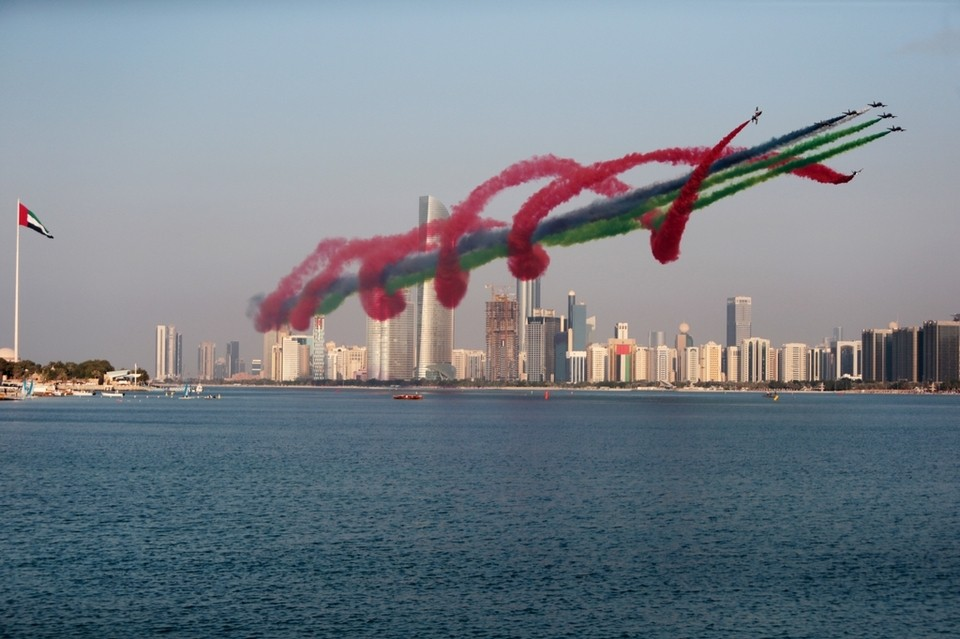
\includegraphics[width=\textwidth]{figures/AlFursan}
		\caption{La patrouille acrobatique émiratie \emph{Al Fursan}, avec ses trajectoires entremêlées mises en évidence par des traînées de fumée colorées. Crédit : The National UAE (\url{http://www.thenational.ae}).}
		\label{fig:alfursan}
	\end{figure}
	
	\paragraph{}
	De même, les hélicoptères militaires sont plus agiles que leurs homologues civils, sans qu'il soit aisé de quantifier cette différence. Comme pour les avions, leur comportement est susceptible d'être  Ils sont ausssi légèrement plus rapides, de quelques dizaines de km/h, notamment en piqué. Comme pour les avions, leurs missions impliquent souvent des trajectoires moins prévisibles.
	
	\paragraph{}
	Le cas des drones aériens, c'est-à-dire des aéronefs sans pilote embarqué (télécommandés ou autonomes) est peut-être le plus hétérogène. On trouve en effet des drones de très petite taille, mais aussi des modèles de plusieurs tonnes~\cite{reaper}. Leurs modes de sustentation sont très divers, leurs moyens de propulsion varient également, et de fait, leurs caractéristiques de vol sont extrêmement variables, des plus petits engins extrêmement manœuvrables jusqu'au plus gros, qui se comportent comme des avions. Au-delà de leurs caractéristiques de vol, certains drones sont délibérément conçus pour être utilisés en grandes quantités, en essaims~\cite{locust, alonso2016distributed, saska2014autonomous}, notamment pour submerger l'ennemi par le nombre. Cela implique une densité de cibles potentiellement très importante, avec les niveaux d'occultation qui en découlent.
	
	\begin{figure}[ht]
		\centering
		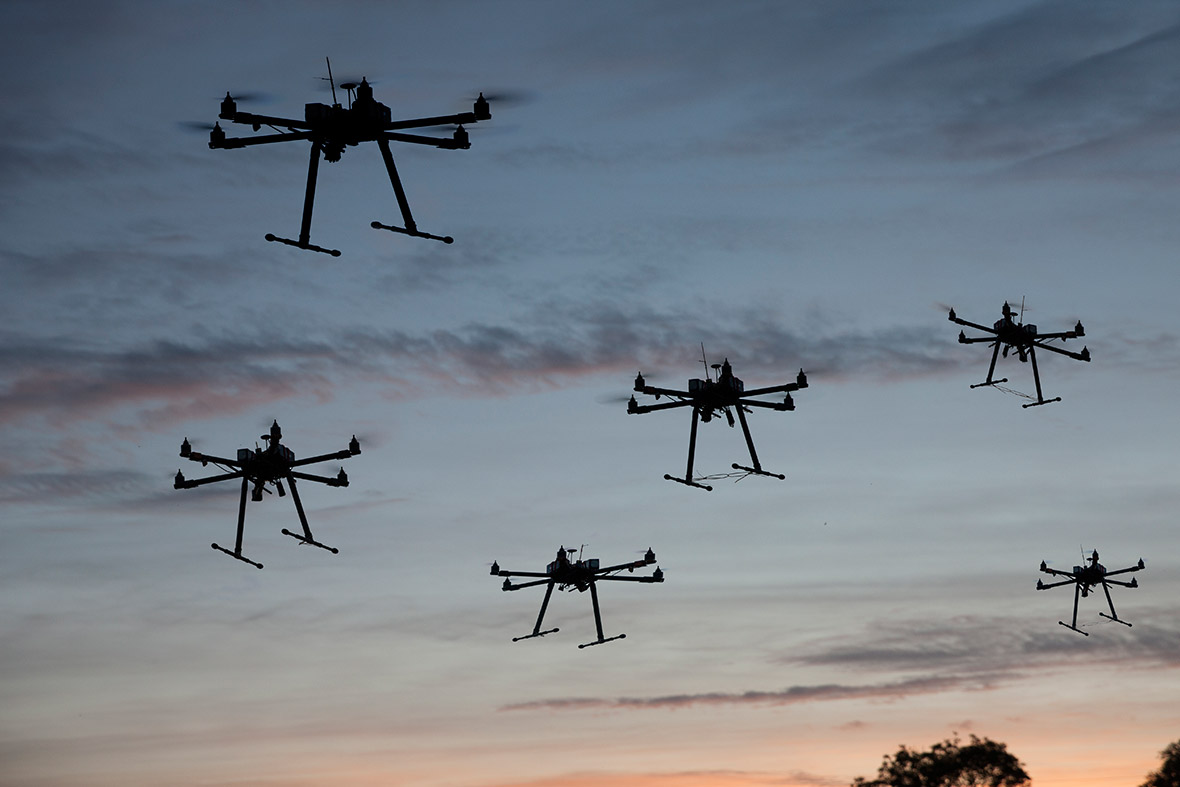
\includegraphics[width=\textwidth]{figures/swarm}
		\caption{Petit essaim de drones aériens. Crédit : \emph{International Business Times}.}
		\label{fig:swarm}
	\end{figure}
	
	\paragraph{}
	Dans une certaine mesure, le contrôle de la circulation des drones est également un enjeu pour le domaine civil, car ils peuvent évoluer (légalement ou non) près des aéroports. Cette pratique peut représenter un risque de sécurité, et des arrêtés ont été pris par le Ministère de l'écologie et du développement durable pour les prévenir, comme le rappelle notamment l'Union des Aéroports Français~\cite{dronesuaf}.
	
	\paragraph{}
	La surveillance de l'espace aérien concerne également divers types de missiles (de croisière, balistiques, etc.). Leurs caractéristiques détaillées sont généralement au moins aussi secrètes que celles des avions de chasse, mais on sait néanmoins qu'ils peuvent être à la fois hypersoniques (c'est-à-dire dépasser Mach~5) et manœuvrables à de telles vitesses~\cite{missiles}, comme le missile BrahMos-II dont une maquette est représentée sur la figure~\ref{fig:brahmos}.
	
	\begin{figure}[ht]
		\centering
		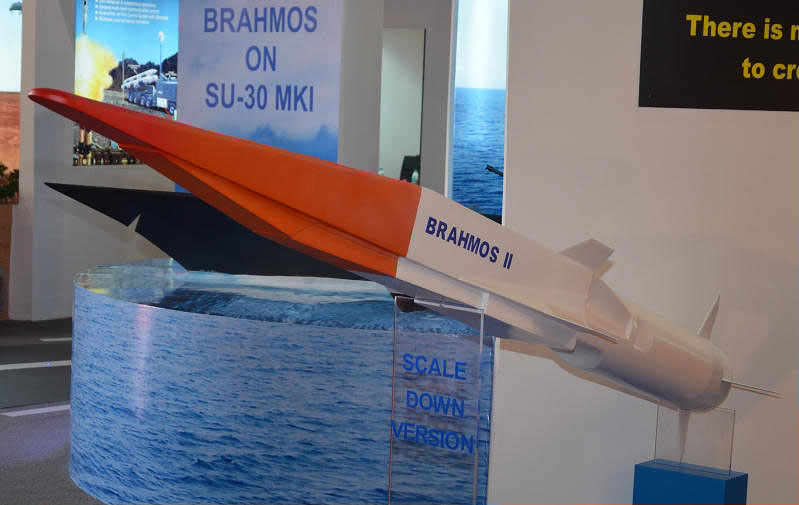
\includegraphics[width=\textwidth]{figures/brahmos-II}
		\caption{Maquette du missile hypersonique russo-indien BrahMos-II, en cours de développement. Crédit : Pakistan Defence (\url{http://defence.pk}).}
		\label{fig:brahmos}
	\end{figure}
	
	\paragraph{}
	En situation réelle, un espace aérien pourrait tout à fait contenir des véhicules et autres engins volants de tous les types sus-cités, des essaims de drones très manœvrables jusqu'aux missiles balistiques les plus rapides. Un système de contrôle interactif devrait donc être assez souple pour permettre la sélection de cibles de natures très différentes.
	On peut noter que les engins volants militaires ont vocation à chercher à éviter d'être détectés, soit en étant naturellement furtifs, soit en volant à très basse altitude et en tirant parti du relief naturel. Il en résulte qu'ils peuvent n'apparaître sur les écrans de contrôle que lorsqu'ils sont déjà très proches de lieux à protéger, et peuvent éventuellement disparaître de ces écrans, offrant une fenêtre temporelle restreinte pour l'interaction.
	
	\subsection{Observations}
	Qu'il s'agisse d'applications civiles ou militaires, cette tâche est critique, puisque de nombreuses vies sont en jeu. Selon l'application, il peut donc y avoir des contraintes fermes et spécifiques, soit sur le temps de sélection maximal acceptable (contrainte de temps-réel) soit sur le taux d'erreur, ou encore sur les niveaux de zoom, etc.

	Les systèmes de contrôle aérien dont nous avons connaissance sont tous en deux dimensions. Pour des engins volants, cela implique nécessairement une perte d'informations. Une technique de sélection suffisamment performante pourrait rendre envisageable l'utilisation d'un système en 3D. Cela permettrait par exemple de mieux déterminer si deux avions qui paraissent dangereusement proches dans le plan le sont réellement dans l'espace, ou de pouvoir choisir un objet parmi plusieurs évoluant aux mêmes coordonnées 2D, mais à des altitudes différentes, ou tout simplement d'avoir une meilleure représentation et perception générales de la situation.

	\begin{figure}[ht]
		\centering
		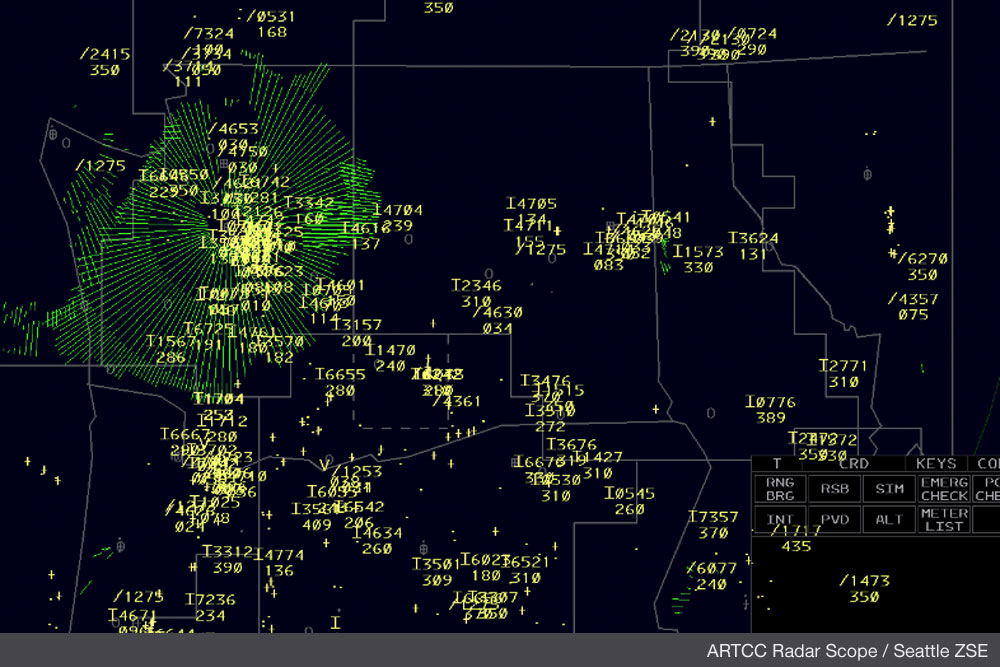
\includegraphics[width=\textwidth]{figures/Radar-Scope-ZSE}
		\caption{Écran de contrôle du trafic aérien. Crédit : \emph{Bold Method}.}
		\label{fig:airtraffic}
	\end{figure}
	
	\section{Vidéo-surveillance}
	La vidéo-surveillance s'applique aussi bien aux foules dans les lieux publics ou sensibles qu'à la voirie, où peuvent circuler des véhicules de types divers. Un agent de sécurité en charge de visionner un flux de vidéo-surveillance pourrait avoir à sélectionner une personne, par exemple pour obtenir des informations sur celle-ci grâce à la reconnaissance faciale, ou un véhicule, pour les mêmes raisons, par exemple grâce à sa plaque d'immatriculation. Quelle que soit la nature de la cible, sa sélection pourrait avoir pour but de zoomer dessus, de verrouiller une caméra robotisée afin qu'elle la suive, ou de la désigner à des forces de sécurité sur le terrain pour qu'elles interviennent physiquement.
	
	\paragraph{}
	La vitesse d'un être humain à pied est inférieure à 45~km/h. Les changements de direction peuvent aller jusqu'au demi-tour, et leur fréquence est très variable selon la tâche accomplie. On peut supposer que cette fréquence est au plus de l'ordre de quelques Hz, en pratique généralement moins.

	\paragraph{}	
	Sur la voie publique, un véhicule motorisé n'est pas censé dépasser 130~km/h, exception faite de ceux qui enfreignent le code de la route. Mais, soit à cause de l'infraction en question, soit parce qu'ils l'enfreignent pour fuir après des délits ou crimes plus graves, ces véhicules-là peuvent justement faire l'objet d'une attention particulière de la part des forces de l'ordre. Dans ces cas-là, la vitesse d'un véhicule peut dépasser les 300~km/h~\cite{speeding}.
	
	Les changements de direction dépendent évidemment de la vitesse. En ville, à moins de 50~km/h, une automobile peut effectuer un virage à 90 degrés dans un laps de temps de l'ordre de la seconde si sa vitesse est réduite, mais elle est contrainte à des courbes beaucoup plus douces lorsqu'elle se déplace rapidement, par exemple sur une autoroute.
	
	La fréquence des changements de direction dépend également de la vitesse, tant pour des raisons physiques que du fait du tracé des trajets communément effectués. En milieu urbain dense, on peut considérer qu'un véhicule va changer de direction, de façon plus ou moins prononcée, à une fréquence de l'ordre de 0,1~Hz, sachant qu'en cas de nécessité, cette fréquence peut être nettement plus élevée.
	
	\paragraph{}
	En plus des piétons et des automobiles, la vidéo-surveillance s'applique à tous les véhicules et moyens de déplacement susceptibles d'être utilisés dans l'espace public : patins à roulettes, skateboards de tous types, bicyclettes, motocyclettes, etc. Les caractéristiques du mouvement de ces moyens de transport sont diverses, mais généralement comprises dans les intervalles formés par les piétons et les automobiles. Il est donc important qu'une technique de sélection puisse non seulement gérer les valeurs extrêmes de vitesse, d'angle et de fréquence de changements de direction, mais également les diverses combinaisons de ces valeurs qui peuvent se présenter simultanément.
	
	\paragraph{}
	Dans certains cas, par exemple au cours de manifestations publiques ou de concerts, les individus filmés peuvent devenir quasi statiques, mais très nombreux et confinés dans un espace réduit. Il en résulte une densité de cibles potentielles et un niveau d'occultation très élevés. Dans ces circonstances, la vidéo-surveillance 
	
	\begin{figure}[ht]
		\centering
		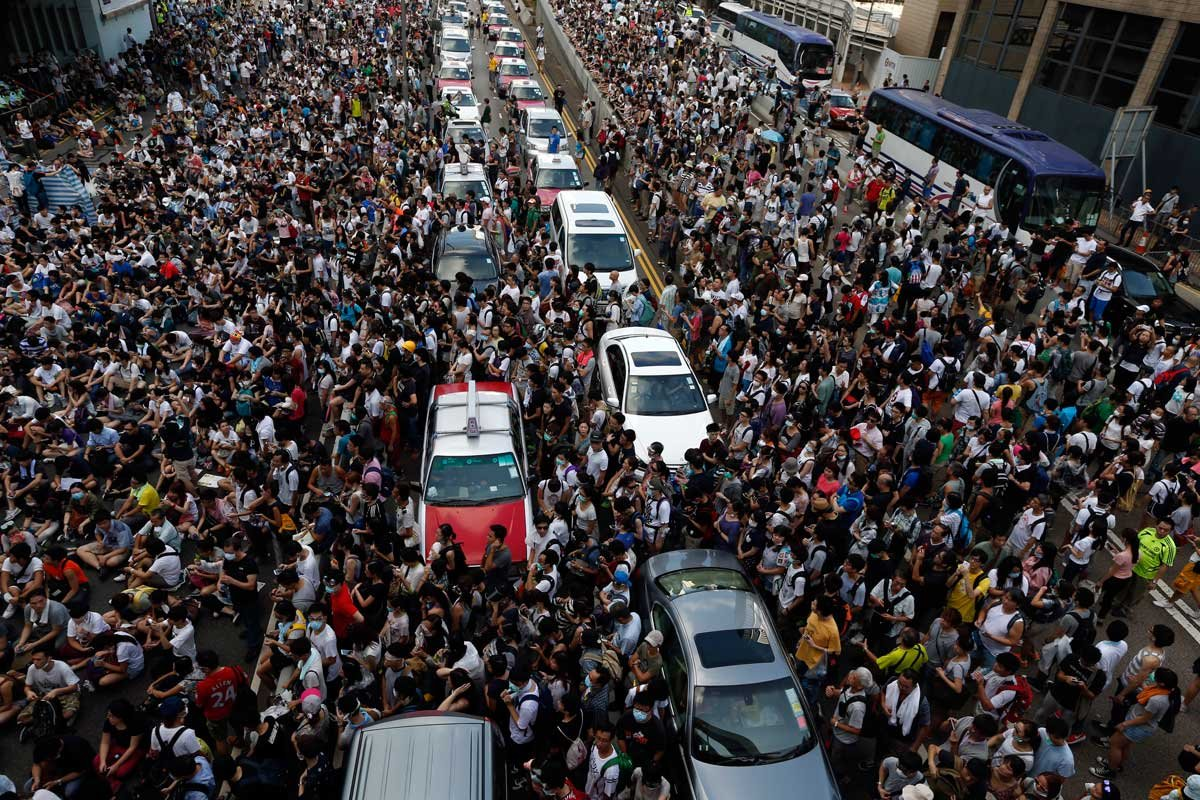
\includegraphics[width=\textwidth]{figures/crowdhk}
		\caption{Foule de manifestants à Hong-Kong. Mouvement très faible, mais densité très élevée. Crédit : \emph{Business Insider}.}
		\label{fig:crowdhk}
	\end{figure}
	
	\begin{figure}[ht]
		\centering
		\includegraphics[width=\textwidth]{figures/crowdacdc}
		\caption{Foule à un concert du groupe AC/DC. Mouvement presque nul, mais densité extrêmement élevée. Crédit : \emph{SHP Online}.}
		\label{fig:crowdacdc}
	\end{figure}
	
	
	
	\section{Analyse de processus complexes}
	
	\section{Retransmissions d'événements sportifs ou artistiques}
	Les retransmissions d'événements sportifs présentent un potentiel d'interactivité intéressant, nécessitant souvent la sélection de cibles mobiles. Il peut être intéressant, par exemple, de sélectionner un joueur de football pour afficher des statistiques. Pour les mêmes raisons, un ballon ou une balle peut être une cible, de même que certains éléments du terrain de jeu, qui sont physiquement fixes mais peuvent être mobiles à l'écran du fait des mouvements de caméra. La nature du mouvement de ces cibles varie nécessairement d'un sport ou d'un jeu à l'autre.
	
	Des sports d'équipe comme le football, le hockey sur glace ou le basket-ball sont caractérisés par des cibles potentielles relativement nombreuses, mobiles, et dont les mouvements ne sont pas toujours très prévisibles. Les courses athléthiques, hippiques, ou les sports mécaniques présentent des mouvement souvent plus prévisibles, mais aussi nettement plus rapides, avec en plus une certaine tendance des cibles à être très proches les unes des autres, ce qui augmente la probabilité d'erreur de sélection.
	
	La vitesse d'un être humain à pied est normalement comprise entre 0 à 45~km/h.
	Changements de direction très imprévisibles et totalement libres
	
	Paramètres beaucoup plus variables pour les projectiles, mais raccourci ?
	
	Cependant, dans la plupart des cas
	
	\section{Jeux vidéo}
	La sélection ou le pointage de cibles mobiles est une tâche que l'on retrouve dans de très nombreux jeux vidéo, appartenant à un nombre important de catégories. On peut notamment citer les jeux de tir (\emph{Fist-person Shooters}, ou FPS), les jeux de stratégie et tactique militaire (les catégories \emph{Real-time strategy} ou RTS, et \emph{Real-time tactics} ou RTT), les simulateurs de vol de combat (réalistes ou non) ainsi que les jeux de type arène de bataille en ligne multijoueur (\emph{Multiplayer online battle arena}, ou MOBA).
	
	
	
	\section{}
    
	Les tendances observées sur les cibles statiques demeurent, à savoir que la difficulté de la tâche augmente quand la distance entre la cible et le pointeur augmente, ou quand la taille de la cible diminue. Mais l'influence du mouvement de la cible empêche d'appliquer la loi de Fitts. Certes, la difficulté de la tâche augmente aussi avec la vitesse, [ref-mec-interact?] cependant, si la nature du mouvement a une importance cruciale, celle-ci demeure peu étudiée.
    
    
    
    
 The
difficulty of the selection increases while (1) target size decreases,
(2) target velocity increases and (3) target density increases. The
selection is even more difficult in 3D environments (filmed or synthetic
environments) because a target of interest can be occluded
by others targets. Selecting someone in crowds with a surveillance
video system is an example of a dense environment with small targets
and occlusion. In some cases, like in action sport footage, both
the objects of interest and the camera can move. Target movements
become unpredictable, and the selection is even more difficult.
In this context, as Hasan et al. [3] wrote, for completing the
selection ”the user must continually track the target and simultaneously
plan to move the cursor over it”. This underscores the key
point of the technique we propose here. Since the user follows the
target for selecting it, the Hook technique tracks the cursor behavior
for assisting the selection. Indeed, observing the history of cursor
displacements, and the history of distances between each target and
the cursor, the system can estimate which target is tracked, and then
propose a selection to the user who just has to validate it. In other
words, the user follows the target of interest, and the system will
know which target it is.
This paper presents the implementation of this technique, and
two experiments which investigate its performance. Hook has been
compared to the basic pointing (non assisted pointing), and to Bubble
cursor [2, 8], for the case of 3D object selection. The first evaluation
involves a desktop configuration, in which pointing is done
on a standard screen with a mouse. The second evaluation involves
an immersive configuration in which pointing is done with a 3dof
(degrees-of-freedom) device. Both evaluations highlight the bene-
fits of this new interaction technique for selecting moving targets in
a 3D environment. More than simply improving the pointing time,
Hook drastically decreases the error rate and allows pointing targets
in high density environments, with high velocity targets that are not
possible to capture with other techniques.


	
		

\clearpage

%!TEX root = these.tex

\chapter[Sélection de cibles : état de l'art]{État de l'art des travaux sur la sélection de cibles}
\minitoc
\label{chap2}
\cleardoublepage

\section{Introduction}
	Dans le présent chapitre, nous ferons d'abord quelques rappels sur la théorie de la sélection de cibles, et un bref état de l'art des modèles existants, en particulier lorsqu'ils sont dédiés aux cibles mobiles. Puis, nous nous attacherons à établir une taxinomie des techniques de sélection les plus connues et/ou performantes. Sans être exhaustif, il s'agit de tâcher d'être représentatif, de mentionner et d'analyser les mérites et limites des principales techniques de sélection.
	
	Cette taxinomie n'a pas vocation à avoir un intérêt universel pour la sélection de cibles, mais elle est établie dans l'optique de la sélection de cibles \emph{mobiles}, et en particulier de cibles mobiles dans des environnements particulièrement difficiles : denses, avec beaucoup d'occultation, de mouvements vifs et imprévisibles, etc. Par conséquent, nos observations sur les différentes techniques citées plus bas seront orientées par la problématique qui nous intéresse, et ne sauraient être prises pour des évaluations absolues des techniques concernées.
	
	De fait, nous séparerons les techniques selon qu'elles seront conçues pour des cibles statiques ou mobiles, tout en admettant qu'une technique appartenant à une catégorie peut généralement être utilisée pour les cibles de l'autre. Ainsi, nous discuterons des techniques de sélection fondées sur un curseur zonal (surfacique ou volumique), sur l'augmentation ou la transformation des cibles, sur l'altération du temps, sur le lancer de rayon ou la projection conique, sur la sélection à plusieurs étapes (dite en cascade), ainsi que sur la prédiction de l'intention de l'utilisateur.
	
	Remarquez que ces catégories ne sont pas mutuellement exclusives, et qu'une technique pourrait tout à la fois utiliser un curseur volumique, augmenter les cibles, éventuellement altérer le temps, se décomposer en plusieurs étapes, et tenter de prédire l'intention de l'utilisateur. La répartition des techniques décrites ici a donc nécessairement quelque chose d'arbitraire, et nous tâcherons d'attribuer à chaque technique une catégorie en fonction de ce qui la distingue le plus des autres, en fonction de ce qui nous paraît être son principe fondamental.
	
	Outre les principes de fonctionnement et mérites apparents des techniques que nous analyserons dans ce chapitre, nous nous attacherons, dans la mesure du possible, à en présenter les performances mesurées empiriquement lorsqu'elle le furent. Il va sans dire qu'aucune étude n'a jamais été menée afin de comparer toutes ces techniques et que, par conséquent, les différentes mesures effectuées ne sont pas toujours directement comparables entre elles. Nous nous attellerons donc à en tirer le plus d'enseignements possible afin d'informer au mieux le lecteur.

\section{Notions théoriques et modèles pour le pointage}
	Le pointage et la sélection de cibles sont de vieux problèmes. Si les cas sur lesquels nous nous concentrons, énumérés dans le chapitre précédent, présentent des difficultés particulières, de nombreuses techniques existent déjà et certaines d'entre elles tiennent compte d'une partie de ces difficultés. L'on peut faire remonter la problématique de la recherche sur le pointage au moins jusqu'à la loi de Fitts~\cite{fitts1954information}. Celle-ci fut établie notamment grâce à une expérience simple, dans laquelle on demandait aux sujets de toucher certaines zones à l'aide d'un stylet, comme illustré par la figure~\ref{fig:fitts}, et détaillé par sa légende.
	
	\begin{figure}[!htbp]
		\begin{subfigure}[t]{0.58\textwidth}
			\centering
			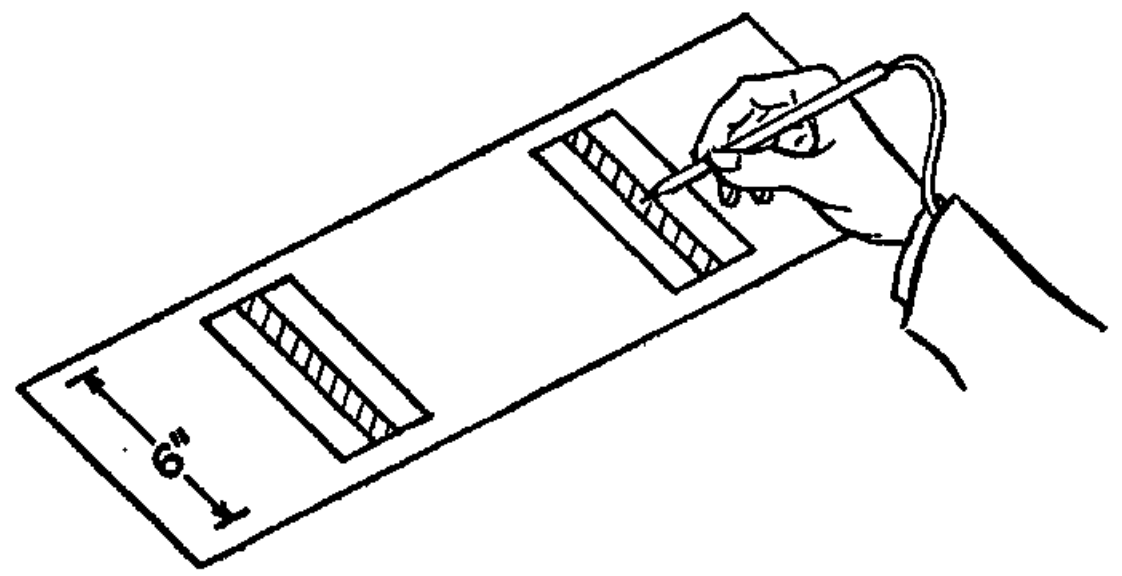
\includegraphics[width=\textwidth]{figures/ch2/fitts}
			\caption{La première expérience ayant mené Paul Fitts à la  définition empirique de la loi du même nom. Deux triplets de plaques étaient séparés d'une certaine distance. Les sujets devaient, avec leur stylet \og tapoter \fg{} alternativement les deux plaques centrales de chaque triplet, hachurées sur ce schéma, sans toucher les plaques adjacentes. On pouvait faire varier la largeur des plaques ciblées, ainsi que la distance entre elles. Crédit : Paul M. Fitts~\cite{fitts1954information}.}
			\label{fig:fitts}
		\end{subfigure}
		~
		\begin{subfigure}[t]{0.40\textwidth}
			\centering
			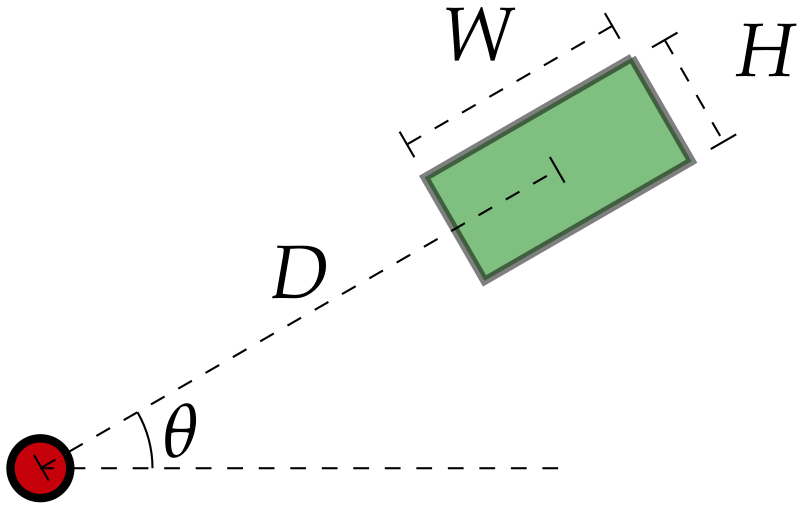
\includegraphics[width=\textwidth]{figures/ch2/theta}
			\caption{Angle $\theta$ pris en compte par~\cite{murata2001extending} dans une version étendue de la loi de Fitts, présentée dans l'équation~\ref{eq:murata}. Le disque rouge représente le curseur, tandis que le rectangle vert représente la cible, située à une distance $D$ du curseur, avec sa largeur $W$ et sa hauteur $H$. Crédit : \cite{casallas2015prediction}.}
			\label{fig:theta}
		\end{subfigure}
		\caption{Expérience de Fitts et modèle de Casallas.}
		\label{fig:fittstheta}
	\end{figure}
	
	Paul M. Fitts a donc pu déduire de cette étude la loi qui porte son nom, et que l'on peut décrire par les équations~\ref{eq:fitts} et~\ref{eq:fittsID}.
	
	\begin{equation}
		\label{eq:fitts}
		T_{M} = a + bID
	\end{equation}
	
	\begin{equation}
		\label{eq:fittsID}
		ID = \log_2\left(\frac{2D}{W} \right)
	\end{equation}
	
	Dans l'équation~\ref{eq:fitts}, $T_{M}$ représente le temps de mouvement, $a$ et $b$ sont des constantes déterminées empiriquement. Dans l'équation~\ref{eq:fittsID}, $ID$ représente l'indice de difficulté, $D$ représente l'amplitude du mouvement, c'est-à-dire la distance entre la cible et le point de départ du mouvement, tandis que $W$ représente la largeur de la cible. La partie la plus intéressante de cette équation est l'indice de difficulté. C'est la seule partie variable, et c'est celle qui, comme son nom l'indique, détermine la difficulté de la tâche. Cet indice est aisé à comprendre intuitivement : plus l'amplitude du mouvement nécessaire est grande, plus la tâche sera difficile ; plus la largeur de la cible est grande, plus la tâche sera facile.
	
	Pour l'indice de difficulté, MacKenzie propose une formulation de l'indice de difficulté dite de Shannon, inspirée de la théorie de l'information proposée par ce dernier~\cite{mackenzie1989note}. Cette formulation, qui a l'avantage d'être positive même quand l'amplitude de mouvement est très faible, est fournie dans l'équation~\ref{eq:shannon}.
	
	\begin{equation}
		\label{eq:shannon}
		ID = \log_2\left(\frac{D}{W} + 1\right)
	\end{equation}
	
	\subsection{Extensions de la loi de Fitts}
	L'étude de Paul M. Fitts portait sur un dispositif mécanique simple, mais sa loi s'applique aussi bien aux périphériques de saisie classiques (souris, \emph{joysticks}, etc.)~\cite{card1978evaluation}. Mieux, alors qu'elle fut d'abord énoncée pour des mouvements sur une seule dimension, cette loi s'étend aisément au plan~\cite{card1978evaluation, mackenzie1992extending}, éventuellement en tenant compte de la forme de la cible~\cite{accot2003refining}, ou même à l'espace tridimensionnel~\cite{murata2001extending}. On peut également généraliser la loi de Fitts pour modéliser des tâches de tracé de trajectoires~\cite{accot1997beyond, accot1999performance}.
	
	Bien que la loi de Fitts soit d'une élégante simplicité et d'une utilité évidente pour modéliser les performances de sélection, de nombreuses formulations plus ou moins différentes existent, et leurs mérites respectifs font débat~\cite{casallas2015prediction}. Certaines extensions peuvent, par exemple, tenir compte de l'angle $\theta$ entre le vecteur qui va du curseur à la cible et un vecteur horizontal orienté vers la droite (cf. la figure~\ref{fig:theta}). C'est le cas de la formulation de~\cite{murata2001extending} exposée dans l'équation~\ref{eq:murata}.
	
	\begin{equation}
		\label{eq:murata}
		ID = \log_2\left(\frac{D}{W} + 1\right) + c \sin \theta
	\end{equation}
	
	D'autres versions tiennent compte simultanément de la forme de la cible et de cet angle $\theta$~\cite{appert2008evaluation, grossman2004pointing}.
	
	\subsection{Loi de Fitts et cibles mobiles}
	La recherche sur la loi de Fitts appliquée aux cibles mobiles, comparativement aux travaux sur les cibles statiques, est très pauvre~\cite{casallas2015prediction}. Elle n'est pas inexistante~\cite{jagacinski1980test, hoffmann1991capture, hajri2011moving} mais très limitée, et elle s'intéresse rarement à la nature du mouvement des cibles, surtout quand ce mouvement est imprévisible. Par exemple, les modèles développés dans les travaux de Jagacinski \emph{et al.}~\cite{jagacinski1980test} ou d'Al Harji \emph{et al.}~\cite{hajri2011moving} font l'hypothèse de cibles de vitesse et de direction constantes.
	
	La loi de Fitts étendue par Jagacinski \emph{et al.} est présentée dans l'équation~\ref{eq:jagacinski}, où $CT$ est le temps de sélection, $D$ et $W$ sont toujours la distance à la cible et sa largeur, $V$ est la vitesse de la cible, tandis que $c$, $d$ et $e$ sont des constantes réelles.
	
	\begin{equation}
		\label{eq:jagacinski}
		CT = c + dD + e(V + 1) \left(\frac{1}{W} - 1\right)
	\end{equation}
	
	Les travaux d'Al Harji \emph{et al.}~\cite{hajri2011moving} vont plus loin en tenant compte de la direction de la cible. Les auteurs ont développé deux modèles basés sur ce principe. Le premier est défini par l'équation~\ref{eq:hajriC2}, où $\vec{F}$ est un vecteur déterminé empiriquement, $\vec{D}$ est le vecteur distance entre le curseur et la cible, $\vec{V}$ est le vecteur de vélocité de la cible, et $\vec{R} = \frac{1}{2} \begin{pmatrix}
	W \\ H \\
	\end{pmatrix}$.
	
	Le second est défini par l'équation~\ref{eq:hajriVW}, où $f_{W'}(\theta)$ est un paramètre empirique dépendant de $\theta$, l'angle formé par la direction du mouvement de la cible et l'horizontale. De même $K$ est un paramètre empirique. $D$ est la distance entre le curseur et la cible, $V$ est la vitesse de la cible, et $W'$ est sa largeur dans la direction du mouvement.
	
	\begin{equation}
		\label{eq:hajriC2}
		ID_{C2} = \log_{2}\left(\abs*{\vec{F} \frac{\vec{D}+\vec{V}}{\vec{R}-\vec{V}}} + 1 \right)
	\end{equation}
	
	\begin{equation}
		\label{eq:hajriVW}
		ID_{VWtW'\theta} = \log_{2}\left( f_{W'}(\theta) \left( \frac{D \pm \frac{V}{K}}{\frac{W'}{2} - \frac{V}{K}} \right) \right)
	\end{equation}
	
	Les corrélations entre ces indices de difficulté et les temps de sélection mesurés par Al Hajri \emph{et al.} sont présentées sur la figure~\ref{fig:holdID}, où l'on observera qu'elles sont très fortes. Néanmoins, ces travaux ne portent que sur des cibles dont la vitesse et la direction sont constantes.
	
	\begin{figure}[!htbp]
		\centering
		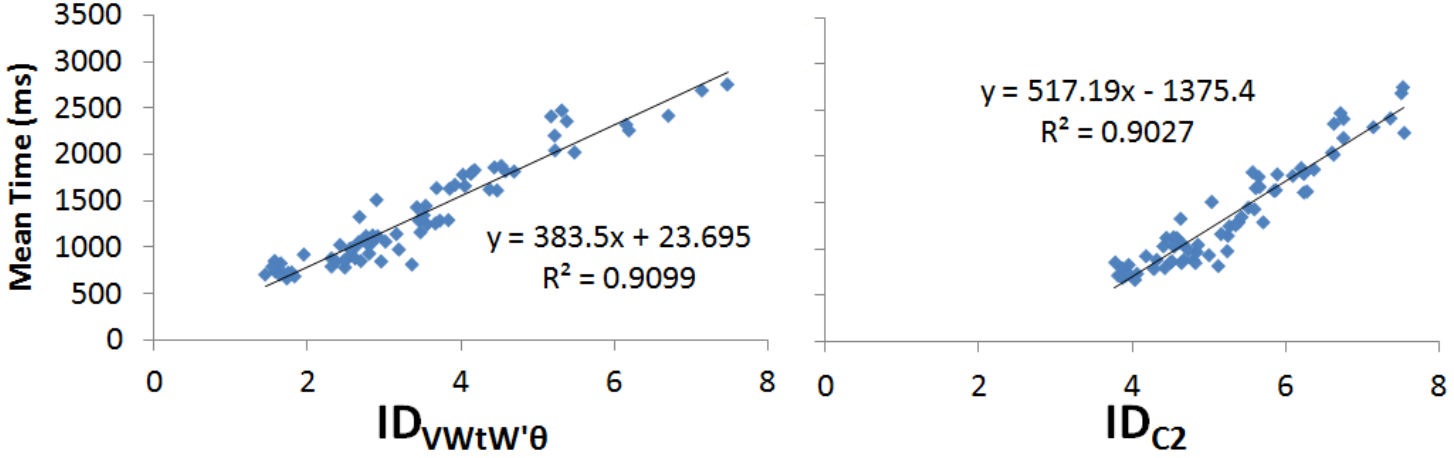
\includegraphics[width=\textwidth]{figures/ch2/holdID}
		\caption[ID vs. nature du mouvement et temps de sélection]{Temps de sélection en fonction des indices de difficulté développés par Al Harji \emph{et al.} Les deux indices sont très fortement corrélés avec les temps de sélection mesurés (sans aucune assistance à la sélection). Crédit : \cite{hajri2011moving}.}
		\label{fig:holdID}
	\end{figure}
	
	Casallas~\cite{casallas2015prediction} a également développé un modèle de prédiction du temps de sélection pour les cibles mobiles, détaillé dans l'équation~\ref{eq:casallas}, où $MT$ est le temps de mouvement, $a_{V}$, $b_{V}$, $c_{V}$ et $d_{V}$ sont des coefficients dépendant linéairement de la vitesse $V$, $D_{m}$ et $D_{s}$ sont les longueurs des composantes orthogonales de $\vec{D}$, le vecteur du curseur à la cible (voir la figure~\ref{fig:casallas}).
	
	\begin{equation}
		\label{eq:casallas}
		MT = a_{V} + b_{V}\sqrt{D_{s}} +  c_{V}\sqrt{D_{m}} + d_{V} \log_{2} \left( \frac{2D_{m}}{W} \right)
	\end{equation}
	
	Dans une évaluation en 3D, l'auteur observe d'une part que l'effet de la vitesse est plus fort que celui de toutes les autres variables, et d'autre part qu'elle réduit l'écart-type des temps de sélection mesurés à mesure qu'elle croît. Il mesure même un très bon ajustement de son modèle aux résultats mesurés, avec le coefficient de détermination $R^{2} \in [0,89 ; 0,96]$.
	
	Il convient cependant de noter un point très spécifique à cette évaluation : les cibles mobiles se dirigeaient toutes \emph{vers} l'utilisateur --- plus ou moins directement. De fait, l'augmentation de la vitesse \emph{diminue} le temps de sélection, puisqu'elle réduit la distance à parcourir pour l'utilisateur, dans un mouvement rectiligne, donc relativement aisé à prédire et anticiper. Ce résultat au demeurant intéressant ne saurait donc suffire à modéliser les performances de sélection pour les cibles mobiles de mouvements quelconques.
	
	\begin{SCfigure}[50][!htbp]
		\centering
		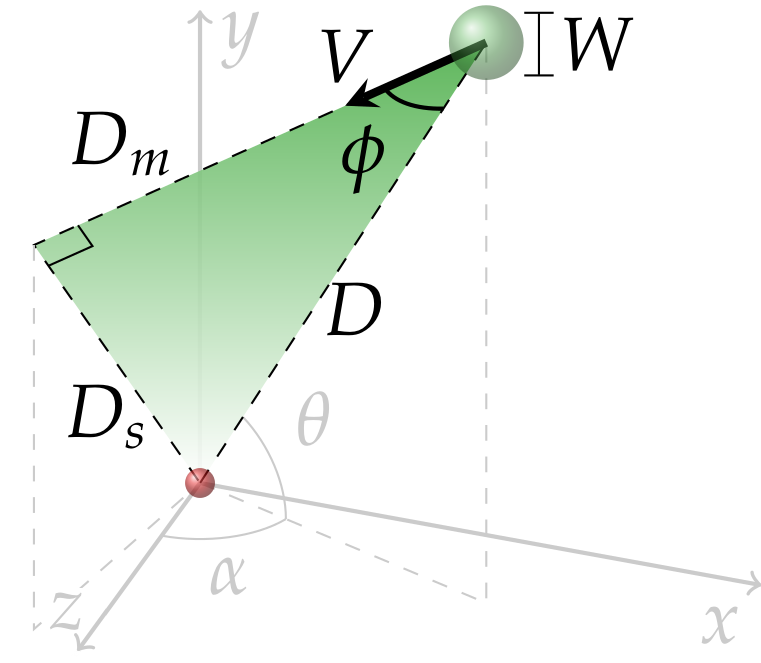
\includegraphics[width=0.28\textwidth]{figures/ch2/casallas}
		\caption[Paramètres du modèle de Casallas]{Modèle de Casallas. $\vec{D}$ est le vecteur du curseur (rouge) à la cible (verte), $\vec{D} = \vec{D_{m}} + \vec{D_{s}}$ où $\vec{D_{m}}$ est la projection de $\vec{V}$ sur $\vec{D}$, et $\vec{D_{s}}$ est la composante de $\vec{D}$ orthogonale à $\vec{D_{m}}$. Crédit : \cite{casallas2015prediction}.}
		\label{fig:casallas}
	\end{SCfigure}
	
	D'autres travaux s'attachent à développer des techniques de sélection de cibles mobiles \og quelconques \fg{} --- c'est-à-dire de direction et de vitesse potentiellement changeantes --- sans nécessairement s'attarder sur les aspects théoriques~\cite{hasan2011comet, ortega2013hook}, et donc sans chercher à étendre la loi de Fitts.
	
	Celle-ci n'a, à notre connaissance, jamais été étendue pour modéliser le temps de sélection de cibles mobiles dont la direction peut changer de façon aléatoire, ce qui la rend d'une utilité discutable pour certaines des applications identifiées plus haut, et particulièrement pour les simulations moléculaires interactives, caractérisées par l'imprévisibilité des mouvements de leurs cibles.
	
	\subsection{Complexité du mouvement : phases balistique et de correction}
	Woodworth~\cite{woodworth1899accuracy} fut à notre connaissance le premier à identifier deux phases dans le mouvement ciblé : une impulsion initiale et une phase de contrôle. Welford~\cite{welford1968fundamentals} fit la même observation et nota par ailleurs que la première phase, visant à couvrir la distance nécessaire, était plus rapide, tandis que la seconde, celle de ciblage, était plus courte~\cite{mackenzie1987three}. Il remarqua de plus, et de même que Crossman et Goodeve~\cite{crossman1983feedback}, que la première phase était \emph{balistique} et qu'à la seconde s'ajoutait un processus de contrôle visuel.
	
	Cela s'observe concrètement dans le profil de vitesse d'un curseur en fonction du temps au cours d'un mouvement ciblé, par exemple de sélection. La phase balistique est caractérisée par une forte croissance suivie d'une forte décroissance de la vitesse, dans un profil pouvant rappeler une cloche ; puis la phase de correction suit, et se distingue par de faibles mais potentiellement nombreuses et surtout rapides oscillations, comme l'illustre la figure~\ref{fig:ballistic}.
	
	\begin{figure}[!htbp]
		\centering
		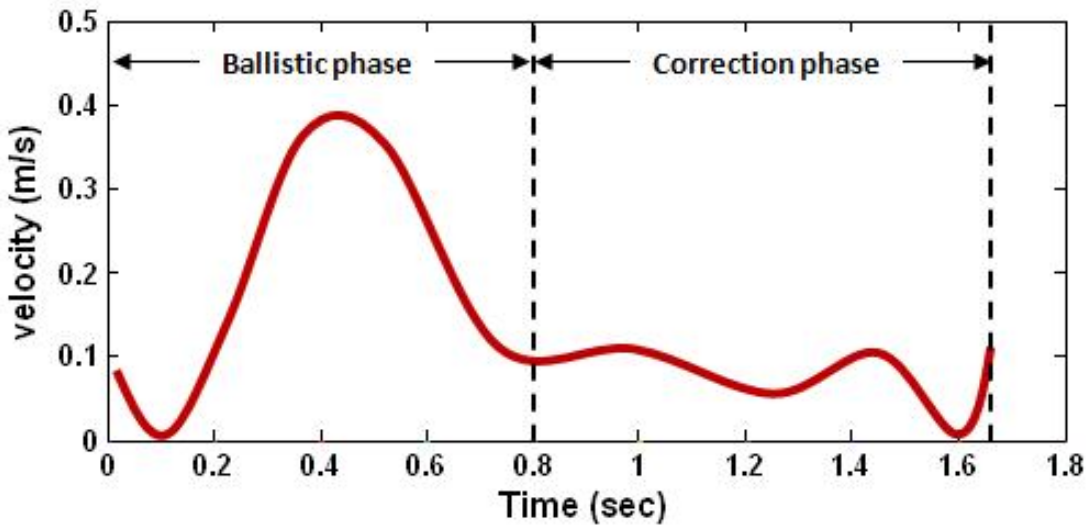
\includegraphics[width=0.70\textwidth]{figures/ch2/ballistic}
		\caption[Profil de vitesse -- phases balistique et de correction]{Vitesse du pointeur en fonction du temps au cours d'un mouvement ciblé. La vitesse croît fortement puis décroît de même au cours de la phase balistique, puis connaît de petites oscillations au cours de la phase de correction. Crédit : \cite{liu2009designing}.}
		\label{fig:ballistic}
	\end{figure}
	
	Langolf \emph{et al.}~\cite{langolf1976investigation} ont de plus montré que \og le mouvement entier vers le centre de la cible devient plus lent quand les tolérances sur la cible (i.e. sa largeur) diminuent \fg{}, ce qui est cohérent avec les travaux de Crossman et Goodeve~\cite{crossman1983feedback}, Marteniuk \emph{et al.}~ \cite{marteniuk1987constraints}, ainsi que ceux de Soechting~\cite{soechting1984effect}. Ce dernier remarqua par ailleurs qu'avec de petites cibles, la phase balistique était plus courte, et de fait la phase de correction en était d'autant rallongée.
	
	La conclusion générale de ces travaux est que la précision requise par un mouvement influe non seulement sur son temps global de complétion, mais également sur l'ensemble de la trajectoire, et notamment sur le profil de vitesse du curseur en fonction du temps. Dès lors, nous pouvons formuler l'hypothèse que les difficultés inhérentes à la sélection de cibles mobiles peuvent être assimilées à un besoin accru de précision, et que par conséquent, un effet comparable pourra être observé sur les trajectoires des curseurs.
	
	Nous reviendrons dans les chapitres suivants sur cette hypothèse.
	
\section{Taxinomie des techniques de sélection}
	Dans les sections suivantes, nous présenterons un échantillon représentatif de techniques de sélection de cibles, statiques et mobiles. Cette présentation sera structurée selon la taxinomie dont un schéma est fourni sur la figure~\ref{fig:selTaxi}, et dont les critères et catégories seront explicités le long des sections suivantes. À la fin du chapitre, un retour global et plus détaillé sur cette taxinomie sera proposé.	
	
\begin{landscape}
	\begin{figure}
		\centering
		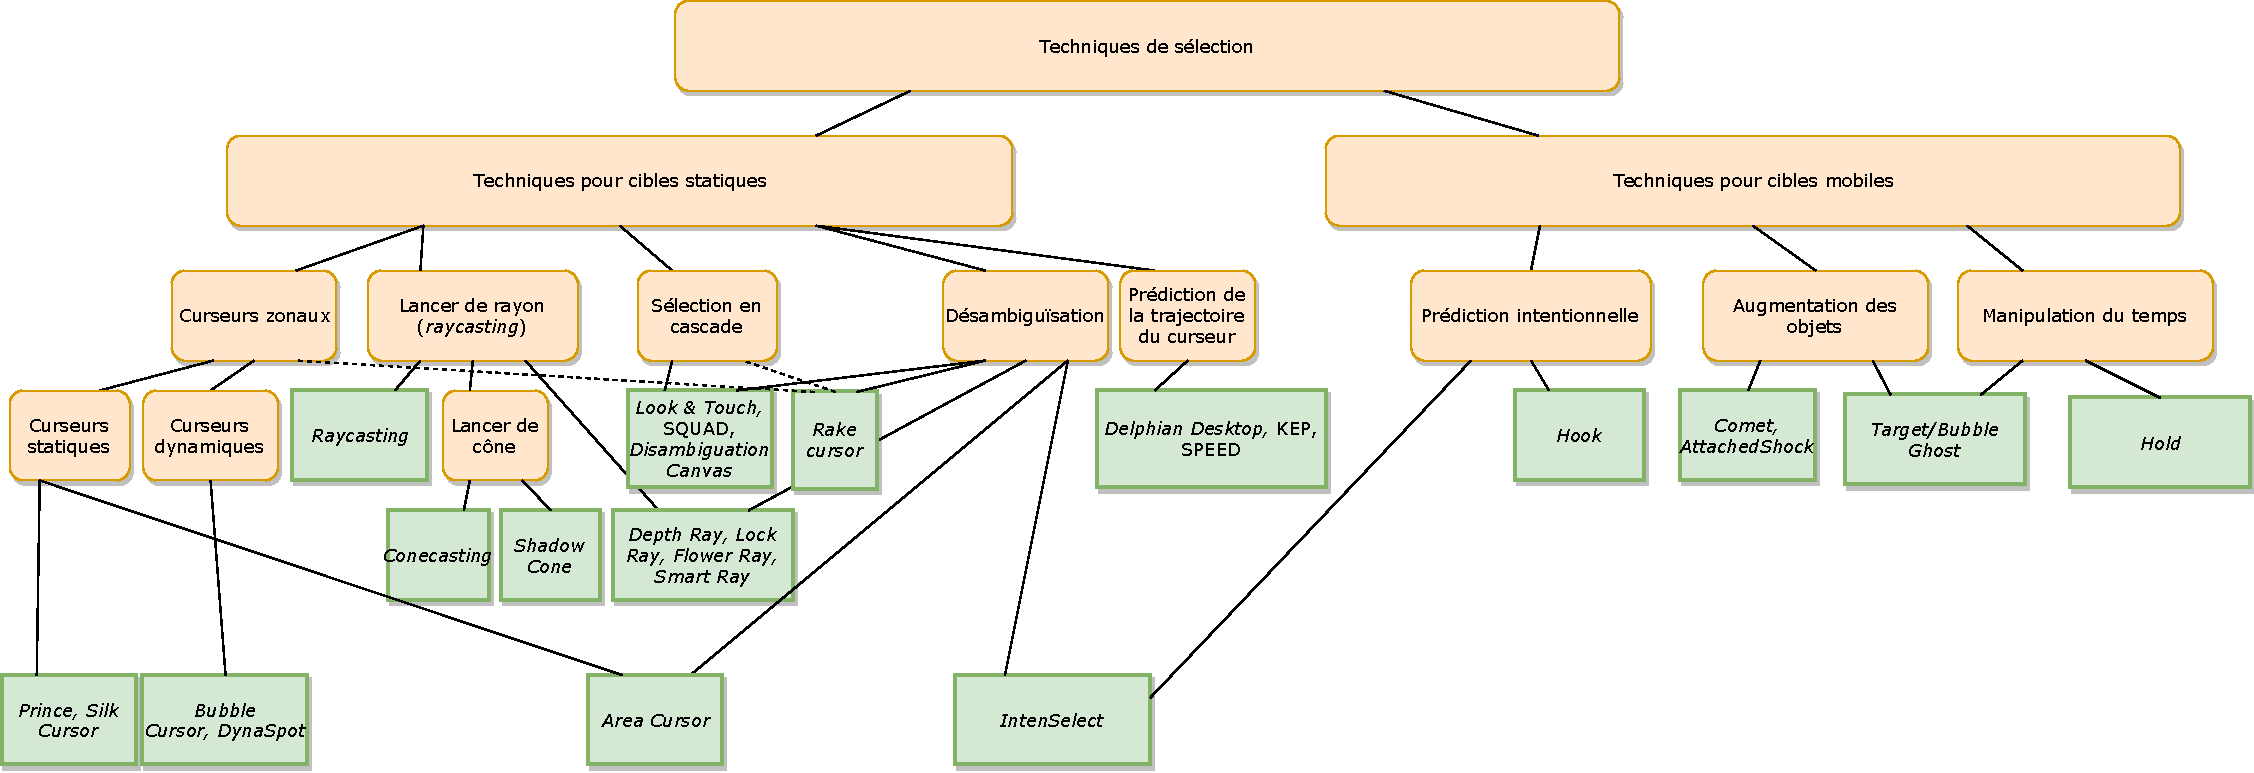
\includegraphics[width=\linewidth]{figures/ch2/selTechTree}
		\caption[Taxinomie des techniques de sélection de cibles]{Notre proposition de taxinomie des techniques de sélection de cibles. Les catégories et sous-catégories sont représentées par des rectangles arrondis de couleur rose pâle, et les techniques de sélection sont représentées par les rectangles bleus/verts. Une technique peut appartenir à différentes catégories à la fois, comme \emph{IntenSelect}, par exemple.}
		\label{fig:selTaxi}
	\end{figure}
\end{landscape}
	
\section{Techniques pour la sélection de cibles statiques}
	Commençons par examiner les techniques conçues pour améliorer les performances de sélection de cibles statiques, mais précisons au préalable qu'elles sont toutes utilisables avec des cibles mobiles, avec divers degrés d'efficacité.

\subsection{Curseurs zonaux}
	Un curseur zonal substitue au curseur ordinaire, qui est réduit à un point, une zone de sélection~\cite{kabbash1995prince, worden1997making}. Lorsque la cible est petite, les performances de sélection ne sont donc plus limitées par sa taille, mais par la taille du curseur. De plus, la distance à parcourir par le curseur zonal pour atteindre la cible est légèrement réduite, puisqu'il faut la mesurer à partir de la limite de la zone de sélection, et non depuis son centre.
	
	\subsubsection{\emph{Prince}}
	La technique \emph{Prince}~\cite{kabbash1995prince} consiste à utiliser un rectangle comme curseur de sélection. Les auteurs ont notamment répliqué la fameuse expérience de Fitts en l'inversant : au lieu d'un point comme curseur et de cibles \og larges \fg{} , ils optèrent pour un curseur large et des cibles ponctuelles, comme l'illustre la figure~\ref{fig:princeCursor}.
	
	\begin{figure}[!htbp]
		\begin{subfigure}[t]{0.56\textwidth}
			\centering
			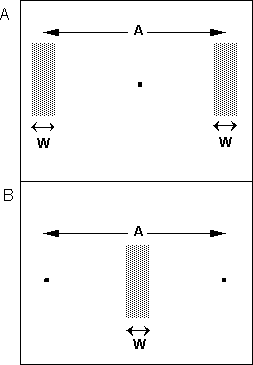
\includegraphics[width=\textwidth]{figures/ch2/princeCursor}
			\caption{À gauche, une représentation schématique de l'expérience de Fitts~\cite{fitts1954information} : un curseur ponctuel est déplacé pour atteindre deux cibles d'aire non nulle. À droite, l'expérience analogue menée dans~\cite{kabbash1995prince}, où le curseur est zonal et les cibles sont ponctuelles.}
			\label{fig:princeCursor}
		\end{subfigure}
		~
		\begin{subfigure}[t]{0.42\textwidth}
			\centering
			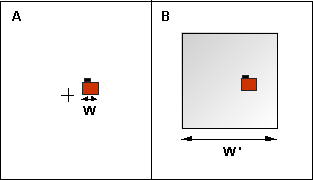
\includegraphics[width=\textwidth]{figures/ch2/princeSelection}
			\caption{Application de la technique \emph{Prince} (à droite) à un cas de sélection pratique, avec pour cible une icône d'aire non nulle ; à gauche, un curseur classique est utilisé.}
			\label{fig:princeSelection}
		\end{subfigure}
		\caption[\emph{Prince}, curseur et sélection]{Crédit : \cite{kabbash1995prince}.}
		\label{fig:princeCursorSelection}
	\end{figure}

	Les auteurs ont pu constater que la loi de Fitts s'appliquait bien à cette configuration, de fait sensiblement identique à celle évaluée par Fitts. Naturellement, dans un environnement de bureau classique, les cibles ne sont pas ponctuelles, mais généralement des icônes ou des boutons d'aire non nulle, comme sur la figure~\ref{fig:princeSelection}, et ce quel que soit le curseur utilisé. De fait, en utilisant un curseur de largeur $W'$, c'est $W'$ qui détermine la difficulté de sélection et non plus la largeur $W$ de la cible (si $W' > w$). Avec un curseur suffisamment gros, l'indice de difficulté peut être considérablement réduit.
	
	La technique \emph{Prince} présente également l'avantage de permettre la sélection de plusieurs cibles d'un coup si elles sont incluses dans le curseur, mais cet avantage reflète une limitation de \emph{Prince}, car il peut dans ces cas-là y avoir ambiguïté si l'utilisateur ne souhaite sélectionner qu'une seule cible.
	
	\subsubsection{\emph{(Sticky) Area Cursor}, \emph{stickiness} et adaptativité}
	Une solution à ce problème d'ambiguïté est proposée par Worden \emph{et al.}~\cite{worden1997making} : lorsqu'un curseur zonal recouvre plusieurs cibles, le curseur devient en pratique un curseur ponctuel, et seul son centre est actif, comme l'illustre la figure~\ref{fig:areaCursor}.
	
	\begin{figure}[!htbp]
		\centering
		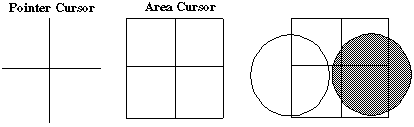
\includegraphics[width=0.70\textwidth]{figures/ch2/areaCursor}
		\caption[\emph{Area Cursor} avec \emph{hot spot}]{Un curseur zonal dont seul le centre, marqué par l'intersection de deux segments, demeure actif lorsque le curseur chevauche plusieurs cibles. Crédit : \cite{worden1997making}.}
		\label{fig:areaCursor}
	\end{figure}
	
	Cette technique simple permet de tirer parti des avantages d'un curseur zonal quand la densité de cibles est suffisamment faibles, sans pour autant souffrir de ses inconvénients lorsqu'elle est élevée, puisque l'on revient alors à un simple curseur ponctuel.
	
	\paragraph{\emph{Stickiness}.}
	À cette solution, Worden \emph{et al.} ont ajouté l'usage de \emph{stickiness} adaptative pour les icônes. Un curseur est dit \emph{sticky} si, lorsqu'il s'approche d'une icône, celle-ci devient \og collante \fg{}. En pratique, le ratio de sensibilité du curseur (la quantité du curseur par rapport à la quantité de mouvement du périphérique de saisie) diminue, ce qui permet d'une part de ralentir le curseur automatiquement, et d'autre part d'affiner les mouvements correctifs permettant la sélection d'une cible lors de son approche.
	
	Le problème des cibles collantes est que lorsque leur densité est élevée, donc en présence de nombreux distracteurs, la trajectoire du curseur se trouve fortement perturbée par ceux-ci, ce qui peut être contre-productif, ou du moins limiter les bénéfices de cette technique. La solution proposée par Worden \emph{et al.} est de ne rendre les cibles collantes que lorsque le curseur est à moins de 30~\%{} de la vitesse maximale qu'il a atteinte au cours de la tâche de sélection courante. L'hypothèse est qu'une sélection commence par une phase de mouvement très rapide et ample, suivie de petits mouvements correctifs plus lents, et que le curseur sera donc relativement lent près de la cible réellement visée par l'utilisateur.
	
	L'\emph{Area cursor}, en particulier complémenté par des cibles collantes et un gain adaptatif, permet un gain de performances important, en particulier avec des utilisateurs âgés, comme le détaille le tableau~\ref{tab:areaCursor}.
	
	\begin{table}
	\centering
	\begin{tabular}{l c c c c}
										& \multicolumn{2}{c}{Jeunes}	&	\multicolumn{2}{c}{Âgés}			\\
										& Temps (ms)	& Taux de succès	& Temps (ms)	& Taux de succès	\\
		Pointeur seul					& 759			& 95,0				& 1893			& 95,0				\\
		Pointeur collant				& 712			& 97,4				& 1869			& 96,3				\\
		Pointeur adaptatif				& 743			& 97,7				& 1485			& 95,5				\\
		\emph{Area cursor} seul			& 639			& 96,9				& 1658			& 96,3				\\
		\emph{Area cursor} collant		& 596			& 97,9				& 1596			& 97,7				\\
		\emph{Area cursor} adaptatif	& 591			& 99,0				& 1203			& 97,9				\\
	\end{tabular}
	\caption[\emph{Area cursor} -- performances]{\emph{Area cursor} : performances mesurées pour des cibles collantes, avec et sans gain adaptatif en fonction de la vitesse du curseur. Les résultats sont comparés avec un curseur ponctuel dans les mêmes conditions, avec des sujets jeunes (23,4 ans en moyenne) et plus âgés (70,1 ans en moyenne). Les performances sont rapportées par le temps de sélection ainsi que le taux de succès (pourcentage de sélections réussies). Le curseur zonal avec cibles collantes et gain adaptatif permet les meilleures performances, surtout avec des sujets âgés. Données tirées de~\cite{worden1997making}.}
	\label{tab:areaCursor}
	\end{table}

	\subsubsection{\emph{Bubble Cursor}}
	La technique \emph{Bubble Cursor} consiste à agrandir dynamiquement un curseur zonal (représenté par un disque) jusqu'à ce qu'il atteigne la cible la plus proche. Mathématiquement, cela revient à construire un diagramme de Voronoï des cibles et à s'appuyer dessus pour la sélection : le \emph{Bubble Cursor} est toujours dans une et une seule cellule du diagramme, et peut sélectionner la cible correspondante, comme l'illustrent les figures~\ref{fig:bubble} et~\ref{fig:voronoi}. De fait, dans sa version pure, il n'est capable de sélectionner que des cibles, pas l'espace entre celles-ci.	

	\begin{figure}[!htbp]
		\begin{subfigure}[t]{0.45\textwidth}
			\centering
			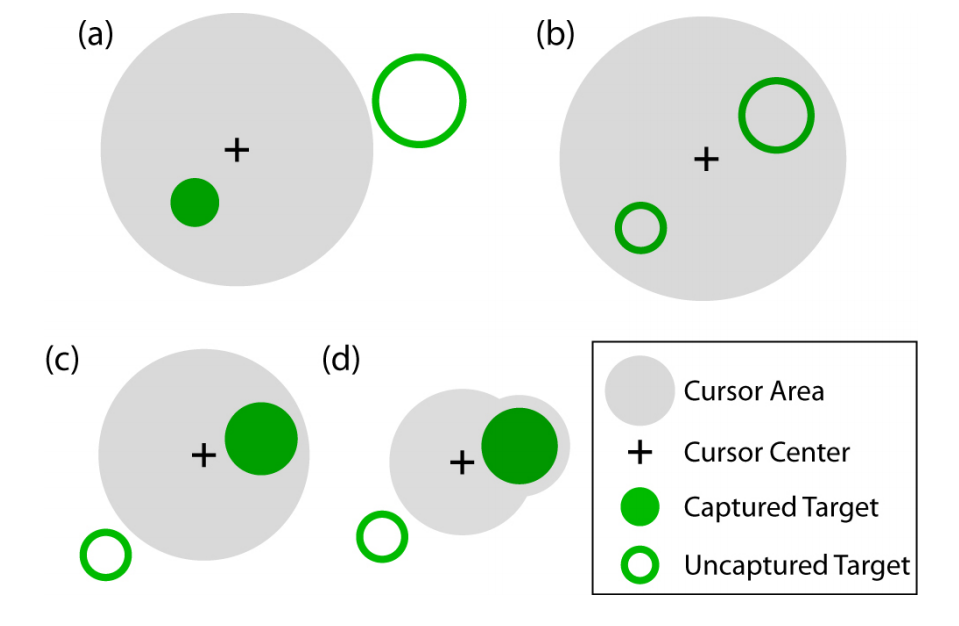
\includegraphics[width=\textwidth]{figures/ch2/bubble}
			\caption{\emph{Bubble Cursor} (a,c,d). (b) : un curseur zonal ne permet pas aisément de choisir entre les deux cibles qui se trouvent dans la zone de sélection, mais le \emph{Bubble Cursor} s'adapte (c et d). (d) : la cible n'est pas \emph{entièrement} recouverte par le disque du curseur, qui est localement étendu pour l'envelopper.}
			\label{fig:bubble}
		\end{subfigure}
		~
		\begin{subfigure}[t]{0.53\textwidth}
			\centering
			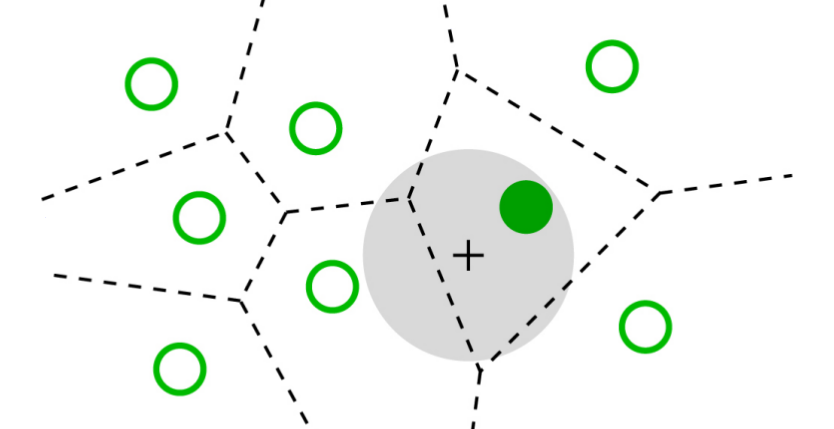
\includegraphics[width=\textwidth]{figures/ch2/voronoi}
			\caption{Diagramme de Voronoï définissant les cellules associées à chaque cible. C'est un pavage du plan en cellules à partir d'un ensemble discret de points (\emph{germes}). Chaque cellule forme l'ensemble des points plus proches de son germe que des autres. Les frontières d'activation de chaque cible, donc sa largeur effective, sont définies par sa cellule.}
			\label{fig:voronoi}
		\end{subfigure}
		\caption[\emph{Bubble Cursor}]{\emph{Bubble Cursor}. Crédit : \cite{grossman2005bubble}.}
		\label{fig:bubbleVoronoi}
	\end{figure}
	
	\begin{SCfigure}[50][!htbp]
		\centering
		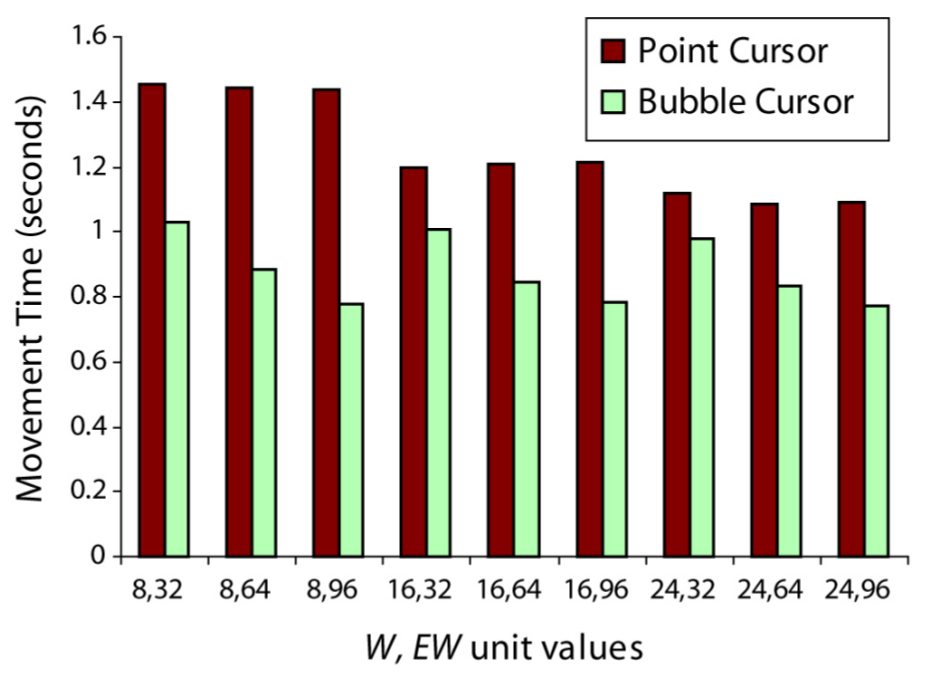
\includegraphics[width=0.42\textwidth]{figures/ch2/bubbleResults}
		\caption[\emph{Bubble Cursor} --  performances]{Temps de pointage avec et sans le \emph{Bubble Cursor}, en fonction de $W$ et $EW$, où $W$ est la largeur réelle de la cible, et $EW$ sa largeur effective. Le \emph{Bubble Cursor} améliore les performances, dépend de $EW$ bien plus que de $W$. Crédit : \cite{grossman2005bubble}.}
		\label{fig:bubbleResults}
	\end{SCfigure}
	
	Grossman et Balakrishnan ont montré que les performances de sélection avec le \emph{Bubble Cursor} suivent la loi de Fitts, à condition de remplacer la largeur de la cible par sa largeur effective, c'est-à-dire la largeur de sa cellule dans le diagramme de Voronoï~\cite{grossman2005bubble}, cf. la figure~\ref{fig:bubbleResults}. Le \emph{Bubble Cursor} peut être mis en œuvre en 2D aussi bien qu'en 3D~\cite{vanacken2007exploring}.

	\paragraph{Instabilité.}
	Un inconvénient de cette technique est le fait que le curseur peut rapidement croître et décroître à mesure qu'il s'approche et s'éloigne de plusieurs cibles successives. Cela peut représenter une source de distraction visuelle, en particulier quand les cibles elles-mêmes sont mobiles, \emph{a fortiori} si elles sont rapides. De plus, attendu que le \emph{Bubble Cursor} agrandit la largeur effective des cibles à la mesure de leur cellule de Voronoï, il est moins efficace en environnement dense, où les cellules de Voronoï sont plus petites. Le \emph{Bubble Cursor} montre donc ses limites face à des cibles potentielles nombreuses, mobiles et rapides. Par ailleurs, un environnement dynamique impose un calcul coûteux~\cite{aurenhammer2000voronoi} de diagramme de Voronoï à chaque déplacement d'un objet.
	
	Un autre inconvénient (potentiellement majeur) du \emph{Bubble Cursor} est intrinsèquement lié à son mode de fonctionnement : il partage l'espace de sélection en un diagramme de Voronoï, où toute partie de l'espace fait partie de la zone de sélection d'une cible. Par conséquent, il n'existe plus d'espace \og vide \fg{} dans lequel on pourrait utiliser le périphérique de saisie pour effectuer une opération indépendante des cibles, par exemple ouvrir un menu contextuel.
	
	\subsubsection{\emph{Silk Cursor}}
	Le \emph{Silk Cursor}~\cite{zhai1994silk} est analogue aux curseurs zonaux décrits plus haut, mais étendu à la 3D. Il s'agit donc d'un volume semi-transparent que l'utilisateur peut utiliser pour sélectionner un objet en déplaçant le volume de telle sorte que l'objet soit dedans.
	
	Tel qu'il fut évalué dans~\cite{zhai1994silk}, le \emph{Silk Cursor} doit entièrement englober un objet pour pouvoir le sélectionner ; ainsi, dans l'illustration de la figure~\ref{fig:silk}, le poisson ne peut pas encore être sélectionné. Celui-ci était animé par une combinaison de fonctions sinusoïdales agissant indépendamment sur chacune de ses coordonnées (x,y,z). Ces fonctions sont détaillées par les équations~\ref{eq:silkMotion0}, \ref{eq:silkMotion1} et~\ref{eq:silkMotion2} où $t$ est le temps, $A = 4,55$~cm, $p = 2$, $f_{0} = 0,02$~Hz, 	$\phi_{x}(i)$, $\phi_{y}(i)$ et $\phi_{z}(i)$ sont des nombres pseudo-aléatoires, échantillonés uniformément entre $0$ et $2\pi$. Ces fonctions ont pour but de produire un mouvement lisse (\emph{smooth}) et subjectivement imprévisible~\cite{zhai1993human}.
	
	\begin{align}
		\label{eq:silkMotion0}
		x(t) &= \sum_{i=0}^{5} Ap^{-i} \sin \left( 2\pi{}f_{0}p^{i}t + \phi_{x}(i) \right) \\
		\label{eq:silkMotion1}
		y(t) &= \sum_{i=0}^{5} Ap^{-i} \sin \left( 2\pi{}f_{0}p^{i}t + \phi_{y}(i) \right) \\
		\label{eq:silkMotion2}
		z(t) &= \sum_{i=0}^{5} Ap^{-i} \sin \left( 2\pi{}f_{0}p^{i}t + \phi_{z}(i) \right) - 7.8
	\end{align}
	
	\paragraph{Temps de sélection.}
	Les performances du \emph{Silk Cursor} furent évaluées par Zhai \emph{et al.} en le comparant à un curseur volumique de fonctionnement identique, mais rendu en fil de fer, dans des conditions monoscopiques et stéréoscopiques (voir la figure~\ref{fig:silkPerf}). Comme le supposaient les auteurs, la semi-transparence du curseur permet une forte amélioration du temps de sélection, particulièrement avec un écran monoscopique. De plus, la stéréoscopie réduit le temps de sélection de façon significative, et ce même avec le \emph{Silk Cursor}.
	
	\begin{figure}[!htbp]
		\begin{subfigure}[t]{0.42\textwidth}
			\centering
			
\includegraphics[width=\textwidth]{figures/ch2/silk}
			\caption{Le \emph{Silk Cursor} : l'utilisateur est ici en train d'essayer de sélectionner un poisson, en l'englobant avec le volume du curseur. Quelques parties du poisson ne sont pas incluses dans le volume de sélection, et de fait il ne peut pas encore être sélectionné.}
			\label{fig:silk}
		\end{subfigure}
		~
		\begin{subfigure}[t]{0.56\textwidth}
			\centering
			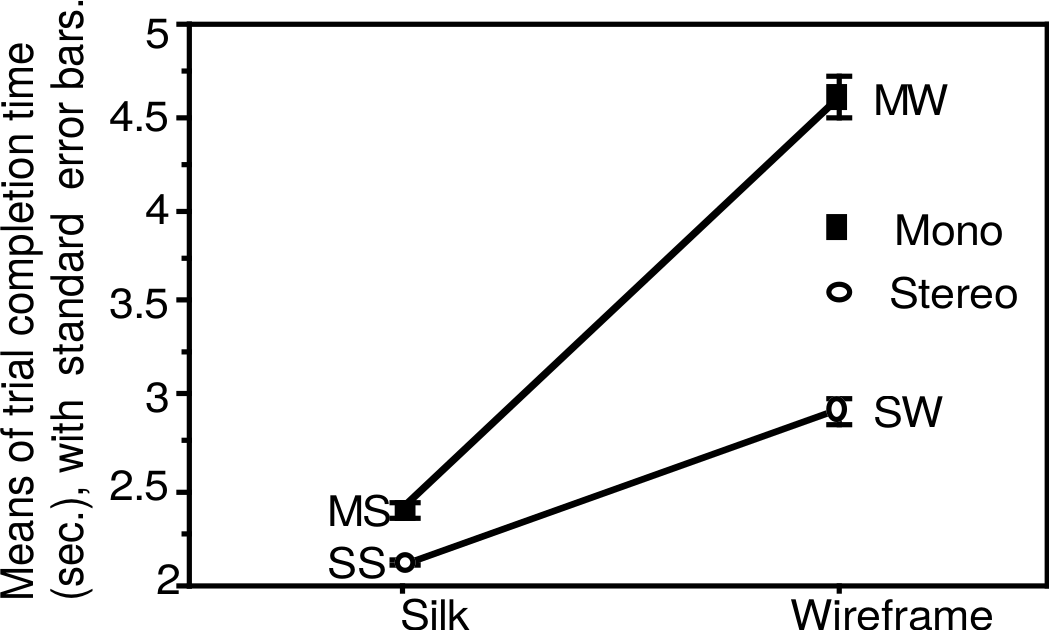
\includegraphics[width=\textwidth]{figures/ch2/silkPerf}
			\caption{Temps de sélection du \emph{Silk Cursor} et d'un curseur volumique en fil de fer. Première lettre : \emph{M} $\rightarrow$ condition monoscopique ; \emph{S} $\rightarrow$ condition stéréoscopique. Seconde lettre : \emph{S} $\rightarrow$ \emph{Silk Cursor} ; \emph{W} $\rightarrow$ curseur en fil de fer (\emph{wireframe}). La stéréoscopie et le \emph{Silk Cursor} améliorent fortement les performances.}
			\label{fig:silkPerf}
		\end{subfigure}
		\caption[\emph{Silk Cursor}]{\emph{Silk Cursor}. Crédit : \cite{zhai1994silk}}
		\label{fig:silkCursorPerf}
	\end{figure}
	
	Observons toutefois que la conception de l'évaluation pourrait favoriser ce dernier de façon artificielle, en ce qu'il est nécessaire que l'objet visé soit intégralement inclus dans le curseur volumique, ce qui ne paraît pas indispensable dans l'absolu. Or, en fil de fer, vérifier cela visuellement est très difficile, tandis que s'assurer qu'une partie de l'objet est dans le curseur semble plus aisé. On peut supposer que la différence de difficulté entre ces deux tâches est moindre avec le \emph{Silk Cursor} grâce aux indications fournies par la semi-transparence, qui facilite la perception de la profondeur et des objets occultés.
	
	\paragraph{Taux et amplitude des erreurs.}
	Les auteurs ont également évalué les performances du \emph{Silk Cursor} en matière d'erreurs, tant pour leur taux d'occurrence (voir la figure~\ref{fig:silkErrors}) que pour leur amplitude (voir la figure~\ref{fig:silkErrorMag}). Cette technique de sélection permet donc d'améliorer les temps de sélection, de réduire les occurrences d'erreurs et de diminuer leur amplitude lorsqu'elles se produisent malgré tout.
	
	\begin{figure}[!htbp]
		\begin{subfigure}[t]{0.49\textwidth}
			\centering
			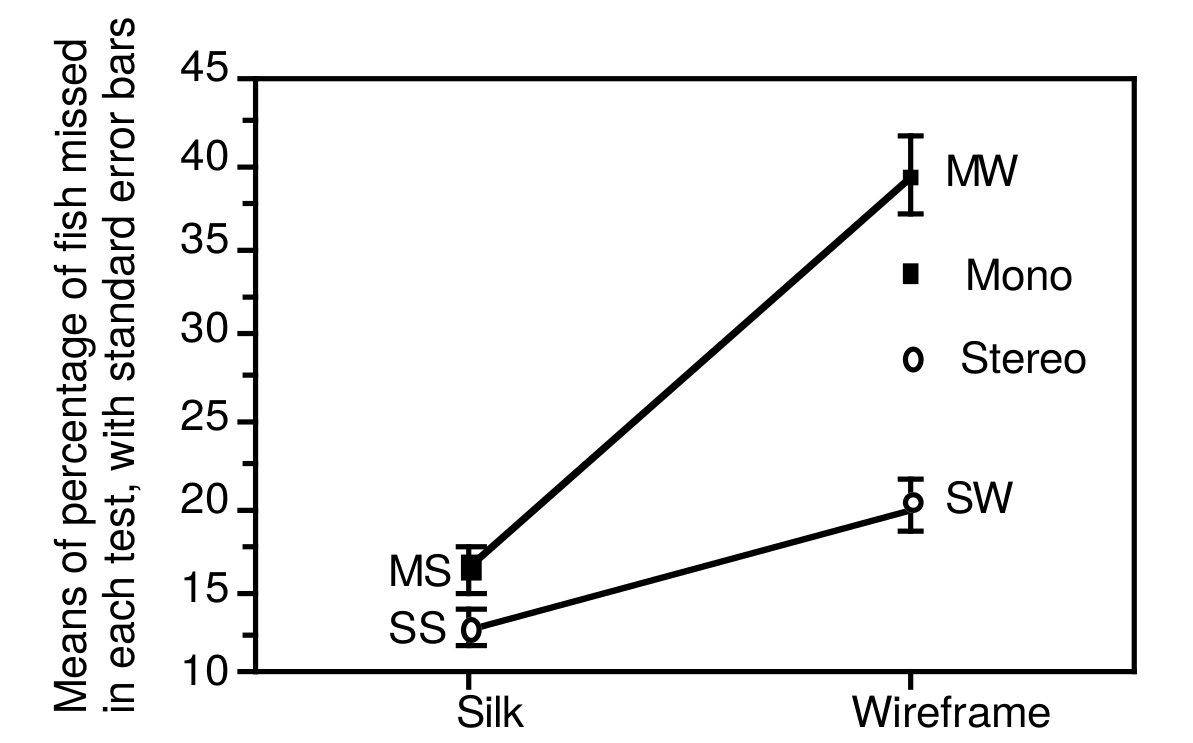
\includegraphics[width=\textwidth]{figures/ch2/silkErrors}
			\caption{Taux d'erreurs du \emph{Silk Cursor} comparé à un curseur volumique. Ici encore, la stéréoscopie et le \emph{Silk Cursor} améliorent les performances.}
			\label{fig:silkErrors}
		\end{subfigure}
		~
		\begin{subfigure}[t]{0.49\textwidth}
			\centering
			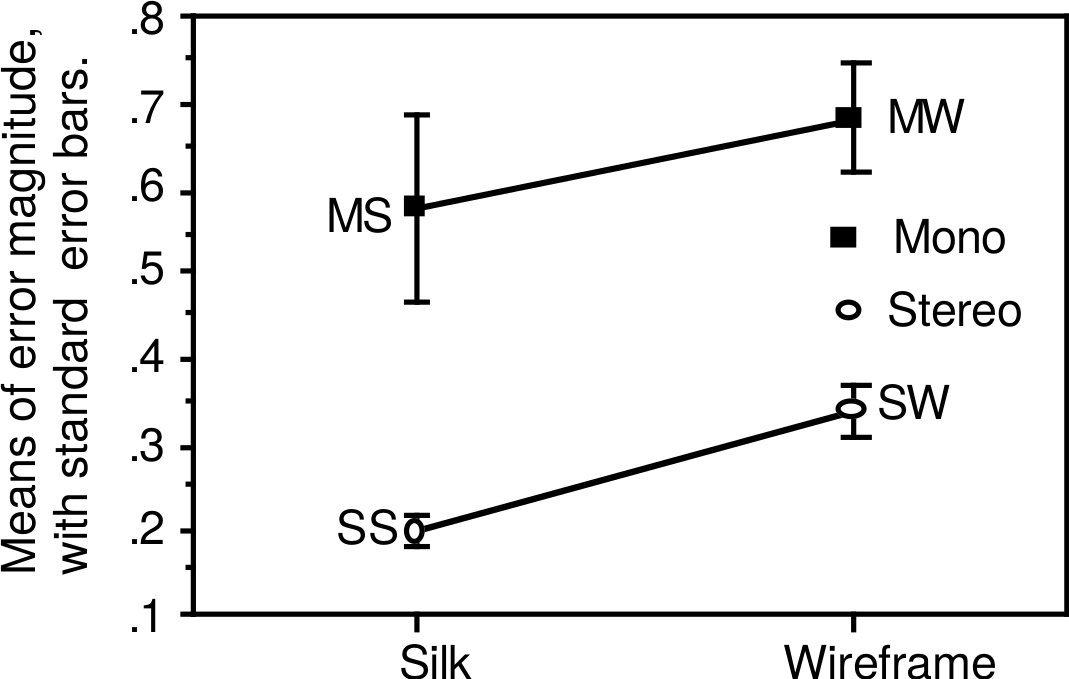
\includegraphics[width=\textwidth]{figures/ch2/silkErrorMag}
			\caption{Erreurs : distance euclidienne entre la position du curseur et celle souhaitée pour saisir la cible. La stéréoscopie et le \emph{Silk Cursor} améliorent les performances.}
			\label{fig:silkErrorMag}
		\end{subfigure}
		\caption[\emph{Silk Cursor} -- Occurrences et amplitude des erreurs]{\emph{Silk Cursor} -- erreurs. Crédit : \cite{zhai1994silk}}
		\label{fig:SilkErrorsErrMag}
	\end{figure}
	
	Enfin, cette étude menée par Zhai \emph{et al.}~\cite{zhai1994silk} confirme l'intérêt du rendu stéréoscopique pour de telles tâches, et montre qu'il apporte toujours un bénéfice tangible lorsqu'il est combiné au \emph{Silk Cursor}.
	
	\paragraph{Impressions subjectives.}
	Zhai \emph{et al.} ont également recueuilli les impressions subjectives des sujets (table~\ref{tab:silkImpr}). Le \emph{Silk Cursor} fut évalué très positivement par les utilisateurs, qui ont même préféré sa version monoscopique à la version stéréoscopique du curseur en fil de fer. En stéréoscopie, toutes les impressions subjectives étaient au moins hautes, et souvent très hautes.

	\begin{table}
	\centering
	\begin{tabular}{c | c c c c c}
							& \multicolumn{5}{c}{Impressions subjectives} \\
		Condition			& Très basse	& Basse	& Moyenne	& Haute	& Très haute \bigstrut[b] \\ \hline
		\emph{MonoWire}		& 8				& 2		& 1			&		& \bigstrut[t]	\\
		\emph{MonoSilk}		& 				& 		& 4			& 4		& 4 			\\
		\emph{StereoWire}	& 				& 2		& 7			& 3		& 	 			\\
		\emph{StereoSilk}	& 				& 		& 			& 3		& 9 			\\
	\end{tabular}
	\caption[\emph{Silk Cursor} -- impressions subjectives]{Impressions subjectives du \emph{Silk Cursor}. Chaque case contient le nombre de sujets ayant évalué la condition correspondante de la sorte. Le \emph{Silk Cursor} s'illustre par les 9 très hautes appréciations reçues en stéréoscopie. Source :~\cite{zhai1994silk}.}
	\label{tab:silkImpr}
	\end{table}

	\subsubsection{\emph{DynaSpot}}
	L'impossibilité de sélectionner l'espace vide avec le \emph{Bubble Cursor} est une des raisons d'être de la technique \emph{DynaSpot}~\cite{chapuis2009dynaspot}. Celle-ci relie l'aire du curseur à sa vitesse. Le curseur conserve sa taille normale lorsqu'il est lent, mais croît et affecte une plus grande surface quand il se déplace plus vite. De fait il suffit de ralentir pour ramener le curseur à un comportement \og normal \fg{} et pouvoir sélectionner de l'espace vide, par exemple pour ouvrir un menu contextuel, ou agir directement sur l'espace vide, comme l'illustre la figure~\ref{fig:dynaSpot}.
	
	\begin{figure}[htbp]
		\begin{subfigure}[t]{0.54\textwidth}
			\centering
			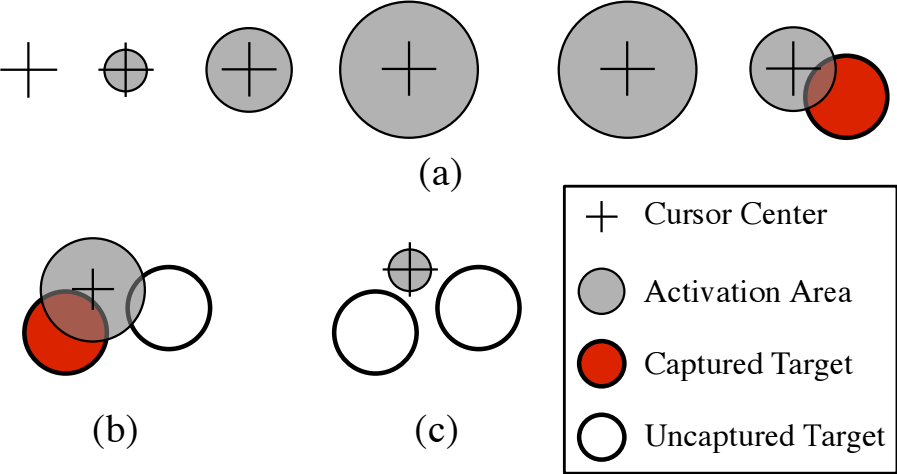
\includegraphics[width=\textwidth]{figures/ch2/dynaSpot}
			\caption{(a) Le curseur de \emph{DynaSpot} croît avec la vitesse du curseur. (b) Plusieurs objets coupent la zone de sélection : la cible la plus proche du curseur est sélectionnée. (c) Quand le curseur ne touche aucun objet, on peut sélectionner l'espace vide.}
			\label{fig:dynaSpot}
		\end{subfigure}
		~
		\begin{subfigure}[t]{0.44\textwidth}
			\centering
			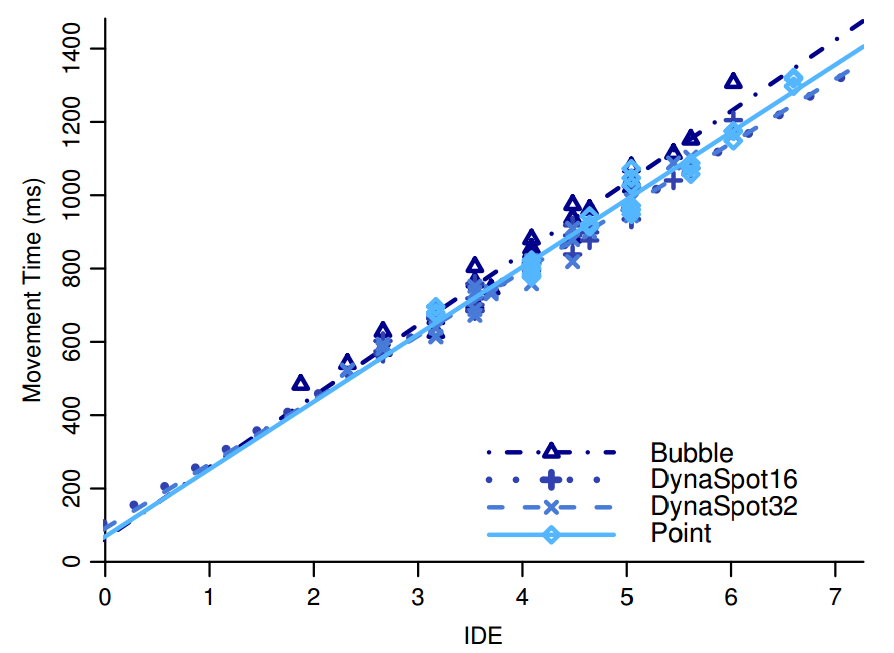
\includegraphics[width=\textwidth]{figures/ch2/dynaResults}
			\caption{Temps de sélection du \emph{BubbleCursor}, de deux versions de \emph{DynaSpot}, et d'un curseur ponctuel, en fonction de l'ID (calculé en fonction de la largeur effective pour le \emph{Bubble Cursor} et \emph{DynaSpot}.}
			\label{fig:dynaResults}
		\end{subfigure}
		\caption[\emph{DynaSpot} -- principe et performances]{\emph{DynaSpot} -- principe et performances. Crédit : \cite{chapuis2009dynaspot}.}
		\label{fig:dynaSpotRes}
	\end{figure}
	
	Il n'est donc pas nécessaire de désactiver \emph{DynaSpot} ou de changer de mode explicitement. En ceci, \emph{DynaSpot} comble une des lacunes du \emph{Bubble Cursor}. Cependant, Chapuis \emph{et al.}~\cite{chapuis2009dynaspot} ont montré que dans la plupart des cas, les performances de \emph{DynaSpot} sont similaires à celles du \emph{Bubble Cursor}. Ces résultats sont résumés dans la figure~\ref{fig:dynaResults}.

	Attendu que la croissance et la décroissance du curseur sont à la fois lentes et prévisibles avec cette technique, le niveau de distraction visuelle est faible. Par ailleurs, il n'est pas nécessaire de connaître la position des cibles potentielles pour appliquer \emph{DynaSpot}, qui ne dépend que de la vitesse du curseur. En cela, cette technique permet de pallier deux autres inconvénients du \emph{Bubble Cursor}.

	\paragraph{Ambiguïté et ralentissements.}
	Le principal inconvénient de cette technique est précisément le fait que le curseur ne tient pas compte des cibles. Par conséquent, à vitesse élevée, sa surface peut en recouvrir plusieurs, et il ne peut déterminer laquelle est la bonne. Il est donc nécessaire de ralentir et d'attendre que le curseur rapetisse suffisamment pour ne toucher qu'une cible. En pratique, cela se produit assez rapidement, et pour les cibles statiques ce n'est pas vraiment gênant. Mais si les cibles sont mobiles, et \emph{a fortiori} rapides, le curseur ne peut s'arrêter, et il peut même être impossible à l'utilisateur de ralentir suffisamment pour que le curseur retrouve une taille permettant la sélection. Ainsi, de même que pour le \emph{Bubble Cursor}, la densité et la vitesse des cibles posent de sérieux problèmes.

	On pourrait toutefois envisager une sélection en deux temps (en cascade) : l'utilisateur pré-sélectionnerait plusieurs cibles lorsque le curseur est gros et rapide, puis devrait choisir parmi les cibles touchées laquelle il veut. Naturellement, le processus de sélection en deviendrait plus lourd et plus long, et pourrait nécessiter de stopper (ou ralentir) les cibles après l'étape de pré-sélection pour que la sélection finale soit réalisable, ou bien encore de zoomer fortement sur l'espace pré-sélectionné. Cette dernière solution semble intéressante, mais pourrait s'avérer peu pratique si les cibles de l'espace pré-sélectionné ont des directions opposées et sont suffisamment rapides pour forcer un \og dézoom \fg{} avant que la sélection finale ne puisse avoir lieu.

	\subsubsection{La densité : un écueil pour les curseurs zonaux}
	Le principal inconvénient d'un curseur zonal se présente lorsque la densité de cibles potentielles est élevée. Si deux cibles sont séparées d'une distance inférieure à la taille de la zone de sélection, il peut être difficile de choisir parmi les deux. Ce problème est illustré par la figure~\ref{fig:bubble}. Il est possible de partiellement pallier ce problème en utilisant une zone plus petite, mais en plus de réduire l'efficacité de la technique, ce n'est certain de fonctionner que si l'on connaît \emph{a priori} la distance minimale entre deux cibles. La figure~\ref{fig:areaCursor} présente une solution possible, qui consiste à n'utiliser que le centre du curseur, mais cela implique la perte de l'avantage fourni par un curseur zonal.
	
	\subsection{Techniques de lancer de rayon (\emph{raycasting})}
	\label{sec:raycasting}
	Certaines techniques substituent aux curseurs classiques des rayons ou volumes projetés depuis un point contrôlé par l'utilisateur. Nous allons ici les examiner ensemble.

	\subsubsection{Lancer de rayon (\emph{raycasting}) pur}
	Le \emph{raycasting} est une technique de sélection conceptuellement très simple : un périphérique est utilisé pour lancer un rayon virtuel, généralement le long d'un axe du périphérique. Le rayon peut ensuite croiser un objet, ce qui permet de le sélectionner. Cette technique est parfois appelée \emph{laser gun}~\cite{liang1994jdcad}, et elle est illustrée par la figure~\ref{fig:dCanvas2}.
	
	Elle a plusieurs avantages : elle permet de sélectionner un objet à n'importe quelle distance, sans avoir à se déplacer ; on peut sélectionner un objet très éloigné de la position initiale du curseur sans avoir à faire de grand mouvement, puisqu'il suffit de changer l'orientation du périphérique de pointage, donc d'un simple mouvement de poignet.
	
	Cependant, pour les objets de petite taille apparente, la sélection peut être difficile, car elle requiert une précision angulaire élevée. De plus, si le système de \emph{tracking} qui fournit la position et l'orientation du périphérique de pointage produit un signal bruité, la difficulté de sélection s'en trouve encore accrue. Par conséquent, des techniques dérivées du \emph{raycasting} ont été développées.
	
	Classiquement, on utilisera une technique de cône de sélection, comme par exemple \emph{Spotlight}~\cite{liang1994jdcad}, illustrée par la figure~\ref{fig:spotlight}. Comme le nom l'indique, les techniques de ce typent remplacent le rayon de sélection par un cône dont le sommet est placé sur le périphérique de pointage.
	
	\begin{SCfigure}[50][!htbp]
		\centering
		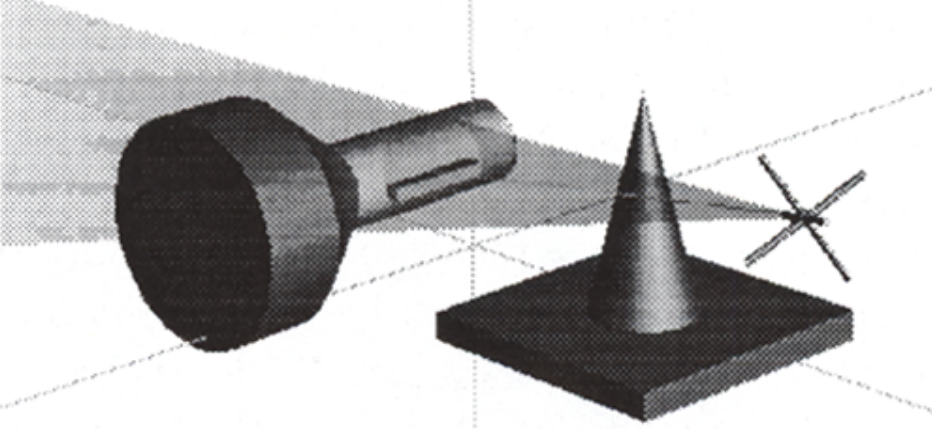
\includegraphics[width=0.44\textwidth]{figures/ch2/spotlight}
		\caption[Cône de sélection : \emph{Spotlight}]{\emph{Spotlight} : les objets dans le cône sont des candidats à la sélection ; quand il y en a plusieurs, le plus proche de l'axe de révolution du cône est choisi, et en cas de proximité égale, le plus proche du périphérique de pointage est choisi. Crédit : \cite{liang1994jdcad}.}
		\label{fig:spotlight}
	\end{SCfigure}
	
	Cela facilite la sélection, puisque les gestes n'ont plus besoin d'être aussi précis, mais peut ajouter de l'ambiguïté si deux objets se trouvent dans le cône de sélection. Le cas échéant, cette ambiguïté peut être levée de plusieurs façon, en fonction de la proximité à l'axe de révolution du cône, en fonction de la distance au périphérique de pointage, ou via une intervention directe de l'utilisateur.
	
	Le choix de l'angle du cône est important : plus il sera grand, plus la sélection sera facile mais potentiellement ambiguë ; plus il sera petit, plus la sélection sera difficile mais spécifique. Le choix de cet angle peut éventuellement être paramétrable, permettant à l'utilisateur de choisir ce qui lui convient le mieux, voire de l'ajuster à la volée en cours d'utilisation. Cet ajustement pourrait également être géré automatiquement par le système interactif, par exemple de façon analogue à ce qui est fait avec des pointeurs classiques dans le \emph{Bubble Cursor}~\cite{grossman2005bubble} ou \emph{DynaSpot}~\cite{chapuis2009dynaspot}.
	
	\subsubsection{\emph{Shadow Cone}}
	Le \emph{Shadow Cone}~\cite{steed20043d} est une technique développée spécifiquement pour les \emph{spatially immersive displays} (SID) tels que les CAVE. L'idée est de permettre non seulement une sélection performante dans des conditions \og normales \fg{} mais également de sélectionner des objets lorsque l'utilisateur n'est pas suivi par le SID, et que le rendu n'est pas adapté à sa position, donc incorrect.
	
	Steed et Parker~\cite{steed20043d} identifient ce besoin en partant du constat qu'un SID ne permet généralement de suivre et d'adapter le rendu graphique qu'à une seule personne (mais pas toujours\footnotemark), ce qui implique qu'un deuxième utilisateur ne peut bénéficier d'un rendu adapté, et rencontrera donc des difficultés pour accomplir des tâches collaboratives nécessitant une étape de sélection.
	
	\footnotetext{Le système EVE (Environnement Virtuel Evolutif), permet d'étudier à la fois les aspects multisensoriels et collaboratifs des interactions humaines au sein de mondes virtuels. Les spécificités du système EVE, comme ses dimensions très grandes, une stéréoscopie multi-utilisateurs haute qualité, des rendus haptiques et audio 3D, en font un dispositif unique au monde à la pointe de la technologie dans le domaine de la réalité virtuelle.
	\url{https://www.limsi.fr/index.php/fr/recherche/venise/menuitem-venise-demos-fr}}
	
	Le \emph{Shadow Cone} fonctionne comme un cône de sélection, mais avec une désambiguïsation explicite : lorsque l'utilisateur presse le bouton de son périphérique de pointage, tous les objets dans le cône sont pré-sélectionnés ; puis, l'utilisateur déplace le périphérique et son cône avec, de telle sorte que certains des objets pré-sélectionnés ne sont plus dans le cône. Dès lors qu'ils en sortent, ils ne sont plus pré-sélectionnés, et aucun objet n'est ajouté à la pré-sélection. Quand l'utilisateur relâche le bouton de son périphérique, tous les objets se trouvant encore dans le cône --- et l'ayant toujours été --- sont sélectionnés. Ce fonctionnement est illustré par la figure~\ref{fig:shadow}.
	
	\begin{figure}[!htbp]
		\centering
		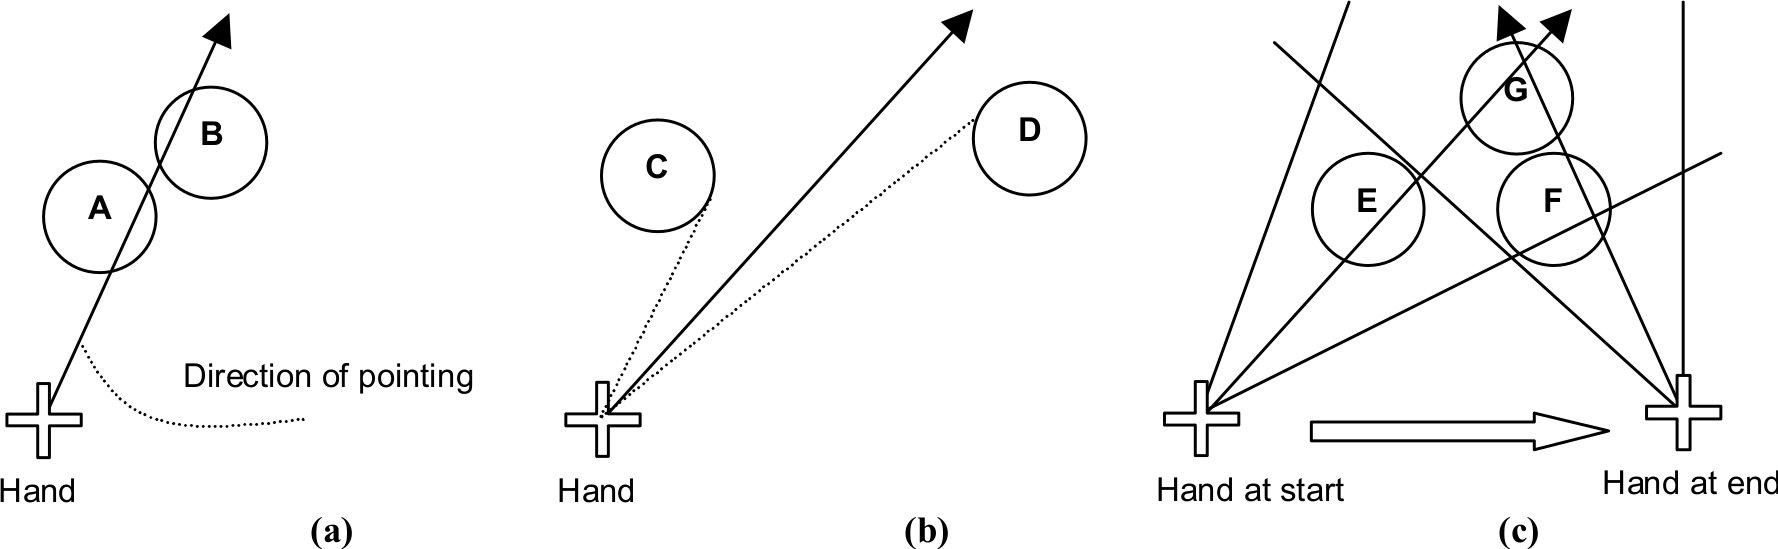
\includegraphics[width=0.9\textwidth]{figures/ch2/shadow}
		\caption[Fonctionnement du \emph{Shadow Cone}]{\emph{Shadow Cone}. (a) Sélection par \emph{raycasting} classique : le premier objet croisé par le rayon est sélectionné (A ici). (b) Sélection par cône : l'objet le plus proche de l'axe de révolution du cône est sélectionné (D ici). (c) \emph{Shadow Cone} : l'objet sélectionné est celui qui est inclus dans le cône de sélection à tous les instants entre la pression du bouton du périphérique et son relâchement (G ici). Crédit : \cite{steed20043d}.}
		\label{fig:shadow}
	\end{figure}
	
	\paragraph{Performances.}
	Steed et Parker ont évalué les temps de sélection du \emph{Shadow Cone}, comparé à la sélection par rayon ou par cône.

	\begin{figure}[!htbp]
		\begin{subfigure}[t]{0.49\textwidth}
			\centering
			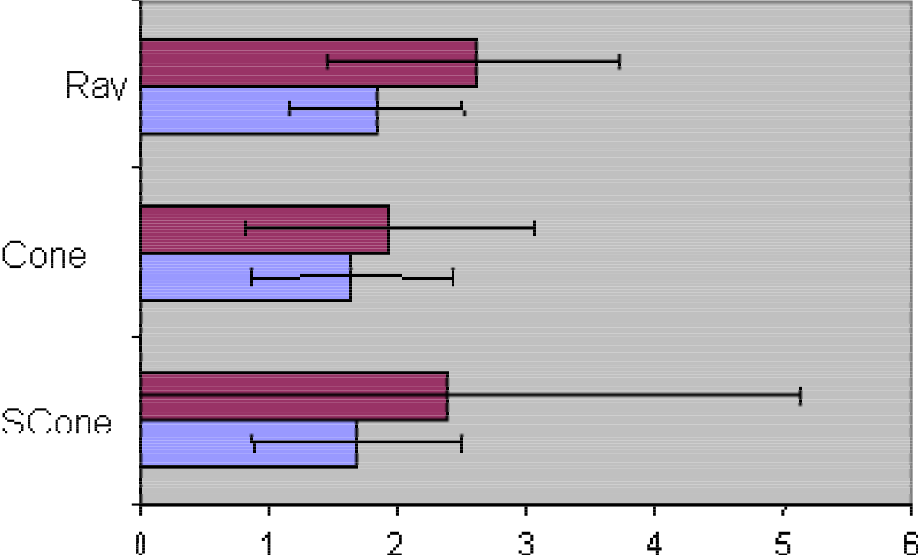
\includegraphics[width=\textwidth]{figures/ch2/shadowSLarge}
			\caption{Grande cible : le \emph{Shadow Cone} ne peut se distinguer des autres techniques.}
			\label{fig:shadowSLarge}
		\end{subfigure}
		~
		\begin{subfigure}[t]{0.49\textwidth}
			\centering
			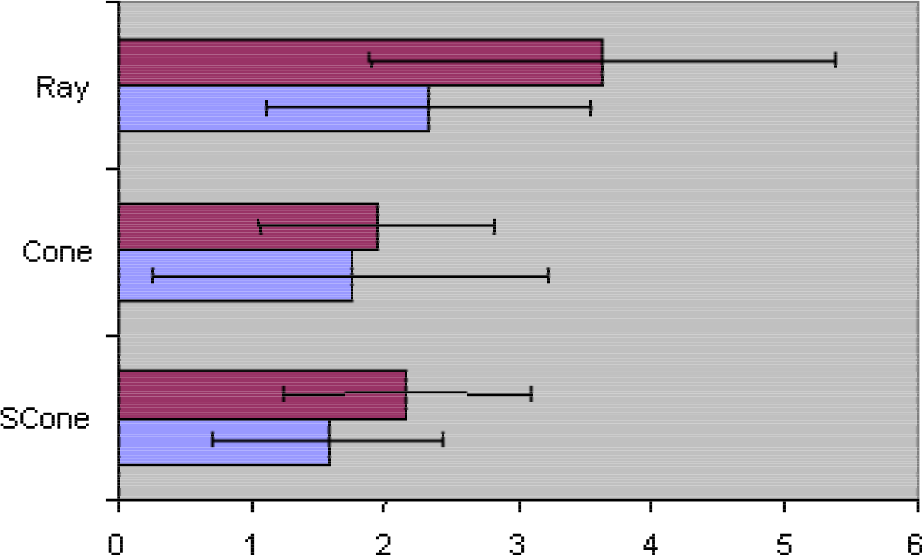
\includegraphics[width=\textwidth]{figures/ch2/shadowSSmall}
			\caption{Petite cible : le \emph{Shadow Cone} ne peut se distnguer de \emph{Cone} ; \emph{Ray} est moins performant.}
			\label{fig:shadowSSmall}
		\end{subfigure}
		~
		\begin{subfigure}[t]{0.49\textwidth}
			\centering
			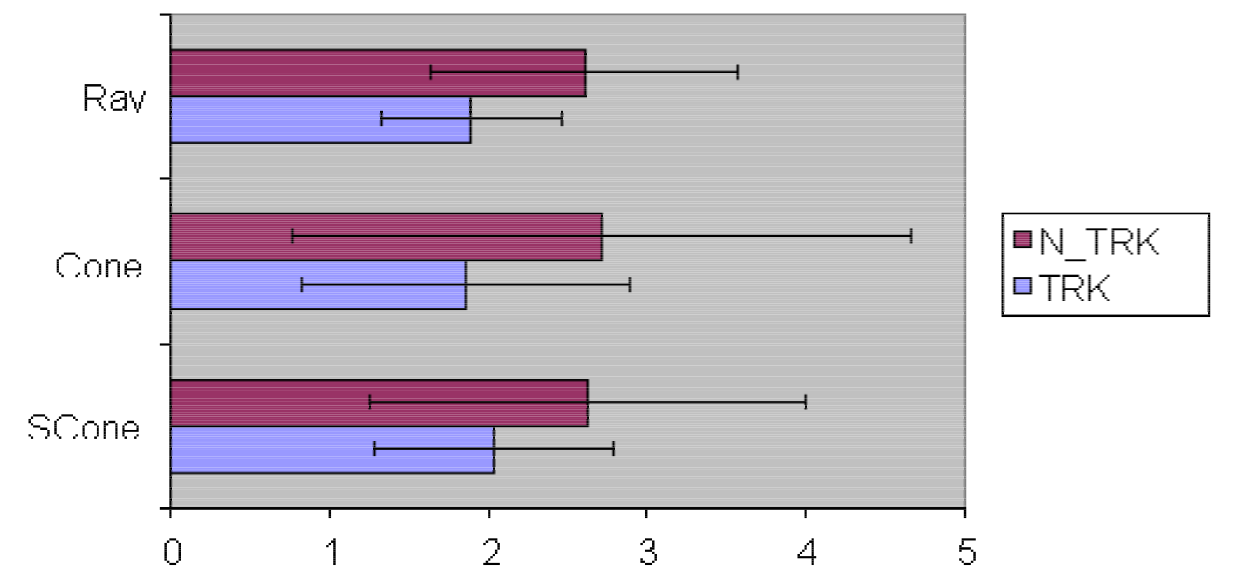
\includegraphics[width=\textwidth]{figures/ch2/shadowPLarge}
			\caption{Paire de grands objets : même temps de sélection pour toutes les techniques. \emph{Ray} : 0 erreur, contre 1,3 erreur/utilisateur pour \emph{Cone}, et 0,2 pour \emph{SCone}.}
			\label{fig:shadowPLarge}
		\end{subfigure}
		~
		\begin{subfigure}[t]{0.49\textwidth}
			\centering
			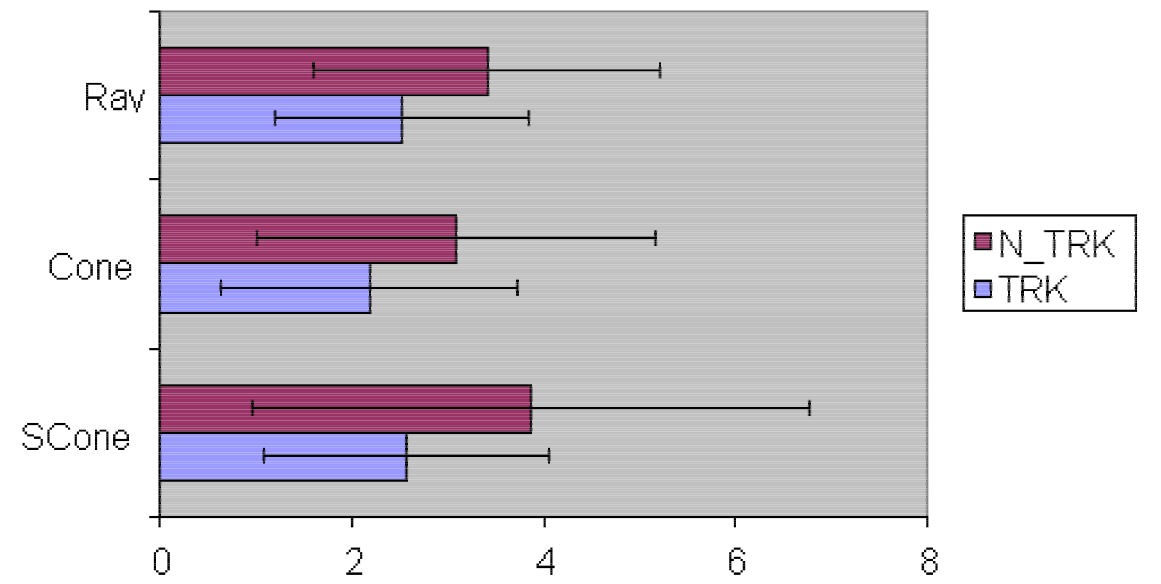
\includegraphics[width=\textwidth]{figures/ch2/shadowPSmall}
			\caption{Paire de petits objets : \emph{SCone} est plus lent que \emph{Cone}, mais génère moins d'erreurs (0,2/utilisateur vs. 0,6) ; aucune erreur pour \emph{Ray}.}
			\label{fig:shadowPSmall}
		\end{subfigure}
		~
		\begin{subfigure}[t]{0.49\textwidth}
			\centering
			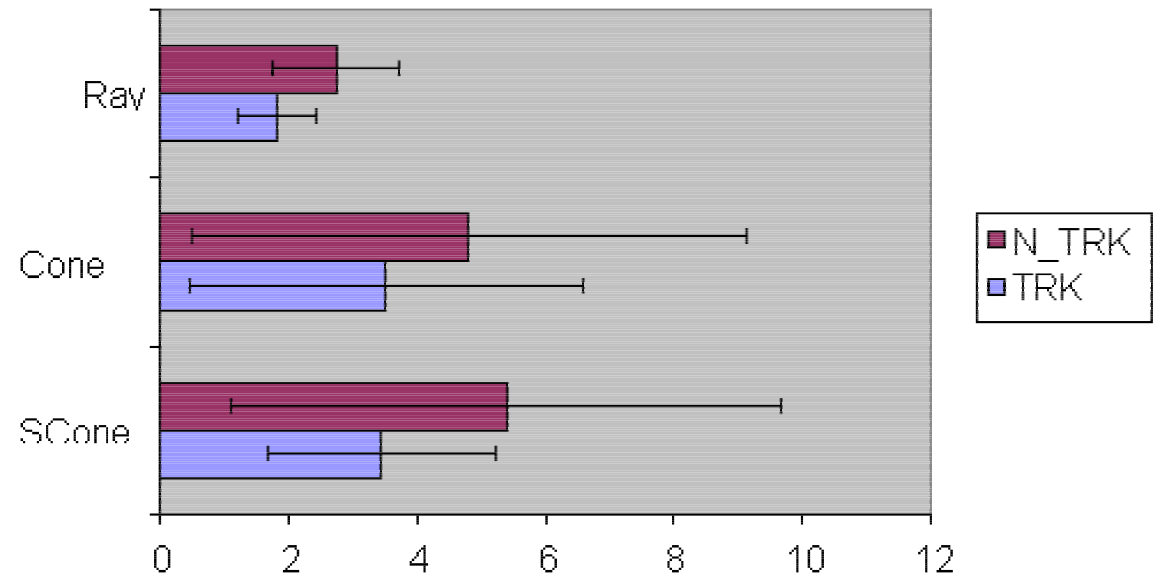
\includegraphics[width=\textwidth]{figures/ch2/shadowCLarge}
			\caption{Grappe de gros objets : \emph{Ray} est plus performant que les autres techniques. \emph{Cone} : 2,2 échecs par \emph{timeout}/utilisateur ; 0 pour les autres techniques. \emph{Cone} : 20,3 erreurs/utilisateur ; 5,2 pour \emph{SCone} et 0,5 pour \emph{Ray}.}
			\label{fig:shadowCLarge}
		\end{subfigure}
		~
		\begin{subfigure}[t]{0.49\textwidth}
			\centering
			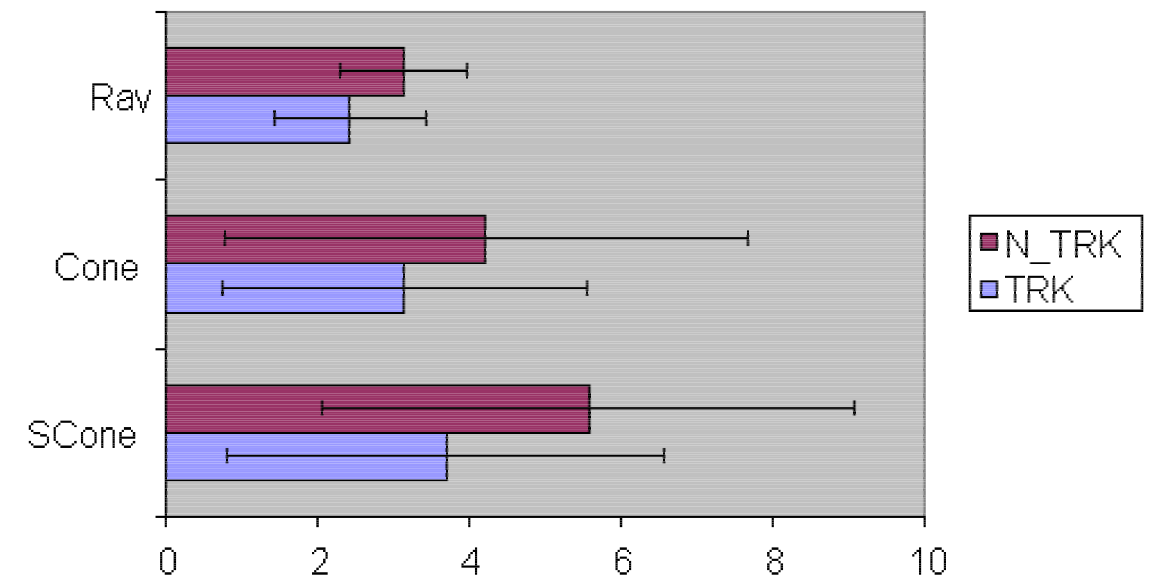
\includegraphics[width=\textwidth]{figures/ch2/shadowCSmall}
			\caption{Grappe de petits objets : \emph{Ray} domine ; pas d'écart significatif entre les autres techniques. \emph{Cone} : 2 échecs par \emph{timeout}/utilisateur ; 0 pour les autres techniques. \emph{SCone} : 4,5 erreurs/utilisateur ; 4,4 pour \emph{Cone}, et 1,2 pour \emph{Ray}.}
			\label{fig:shadowCSmall}
		\end{subfigure}
		\caption[Performances du \emph{Shadow Cone}]{Performances du \emph{Shadow Cone (SCone)}, comparé à la sélection par cône (\emph{Cone}) et par lancer de rayon (\emph{Ray}). Chaque technique est évaluée avec suivi de la tête (en bleu) et sans (en violet) ; les erreurs sont rapportées pour les conditions avec suivi. Crédit : \cite{steed20043d}.}
		\label{fig:shadowConePerf}
	\end{figure}
	
	Les temps de sélection mesurés pour les différentes techniques, avec et sans suivi de la tête, sont présentés sur la figure~\ref{fig:shadowSLarge} pour une grande cible seule, la figure~\ref{fig:shadowSSmall} pour une petite cible seule, la figure~\ref{fig:shadowPLarge} pour une grande cible avec un distracteur, la figure~\ref{fig:shadowPSmall} pour une petite cible avec un distracteur, la figure~\ref{fig:shadowCLarge} pour une grande cible avec de nombreux distracteurs, et enfin la figure~\ref{fig:shadowCSmall} pour une petite cible avec de nombreux distracteurs.
	
	Quoique les figures sus-citées présentent les résultats avec et sans suivi de la tête, nous nous contenterons ici de commenter les résultats avec suivi, attendu que le cas particulier de rendu immersif incorrect dans un SID dépasse le cadre de cet état de l'art, et n'est pas particulièrement pertinent au regard des besoins et applications identifiés au cour du premier chapitre. Observons simplement que, pour une condition et une technique données, le suivi de la tête améliore toujours les temps de sélection, comme l'on pouvait s'y attendre ; l'effet sur les erreurs et échecs est généralement le même.
	
	\subsubsection{Le problème de l'ambiguïté en environnement dense}
	Lorsque l'environnement est particulièrement dense, la sélection par rayon ou cône devient difficile~\cite{kopper2011rapid}, car la précision requise devient très élevée, tant pour l'utilisateur que pour le système de suivi du périphérique de pointage. L'utilisation d'un cône facilite la sélection de petites cibles, mais ajoute un risque d'ambiguïté. Une solution pourrait être d'augmenter le ratio contrôle/affichage à proximité des cibles~\cite{frees2007prism, kopper2010human}, mais c'est au prix de l'introduction d'un décalage entre l'orientation réelle du périphérique de pointage et celle du rayon lancé, ce qui peut être très troublant, et peu performant avec des cibles mobiles, surtout rapides.
	
	Et si diverses techniques peuvent aider à lever l'ambiguïté, leur utilisation est d'autant plus difficile que les cibles situées dans le volume du cône sont nombreuses, petites et\ldots{} mobiles. En effet, la mobilité des cibles nécessite d'effectuer des mouvements plus rapides pour les pointer, donc d'exercer plus de force, et de fait, d'être moins précis~\cite{schmidt1979motor}. En particulier, le \emph{Shadow Cone} impose de maintenir la cible visée à l'intérieur du cône pendant toute la phase de désambiguïsation, ce qui peut s'avérer extrêmement difficile avec une cible en mouvement, \emph{a fortiori} si ses mouvements sont rapides et/ou imprévisibles. Par conséquent, nous ne pouvons retenir cette technique pour les applications qui nous intéressent.
	
	Néanmoins, observons qu'en assouplissant quelque peu cette contrainte, le \emph{Shadow Cone} fournirait potentiellement de meilleurs résultats avec les cibles mobiles. C'est en substance ce que propose le \emph{Smart Ray}~\cite{grossman2006design}, décrit plus bas.

	\subsection{\emph{Raycasting} avec désambiguïsation}
	Dans~\cite{grossman2006design}, Grossman \emph{et al.} proposent d'évaluer diverses techniques de sélection dérivées du \emph{raycasting} et ayant pour but de faciliter la désambiguïsation lorsque le rayon atteint plusieurs objets. Ces travaux sont présentés comme étant motivés par l'émergence d'écrans volumétriques\footnotemark{}~\cite{ebert1999realizing}, mais demeurent très pertinents pour des dispositifs d'affichage plus classiques, notamment stéréoscopiques.
	
	\footnotetext{Un écran volumétrique est un dispositif formant une représentation en 3D des objets qu'il affiche, généralement via une forme d'autostéréoscopie, c'est-à-dire de stéréoscopie ne nécessitant pas le port de lunettes spéciales.}

	\subsubsection{\emph{Depth Ray}}
	Le \emph{Depth Ray}~\cite{grossman2006design} fonctionne comme une technique de \emph{raycasting} traditionnelle, si ce n'est que la position du périphérique le long de son axe de pointage est prise en compte, comme le montre la figure~\ref{fig:depthRay}. Le rayon est ainsi augmenté d'un marqueur de profondeur que l'utilisateur déplace le long du rayon simplement en avançant ou en reculant le périphérique de pointage.
	
	\newcommand{\rayWidth}{0.48\textwidth}
	\begin{figure}[!htbp]
		\begin{subfigure}[t]{\rayWidth}
			\centering
			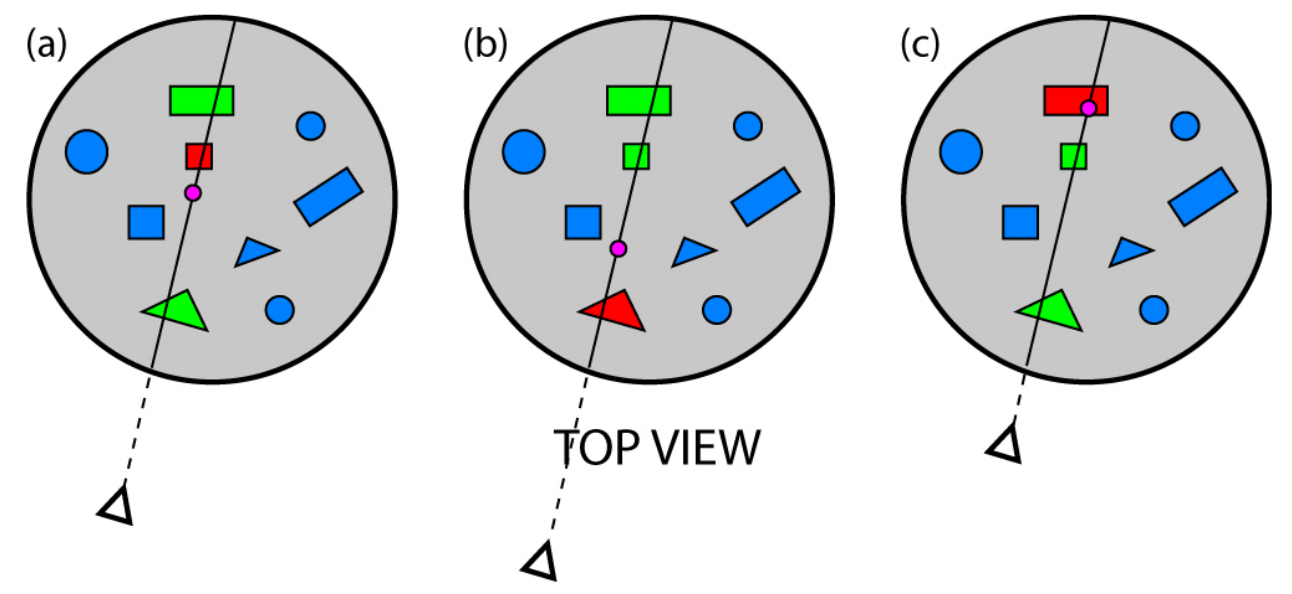
\includegraphics[width=\textwidth]{figures/ch2/depthRay}
			\caption{\emph{Depth Ray}. (a) Un marqueur rose sélectionne la cible intersectée la plus proche de lui. (b) Reculer le périphérique de pointage recule le marqueur et permet de séletionner une cible plus proche\ldots{} et inversement (c).}
			\label{fig:depthRay}
		\end{subfigure}
		~
		\begin{subfigure}[t]{\rayWidth}
			\centering
			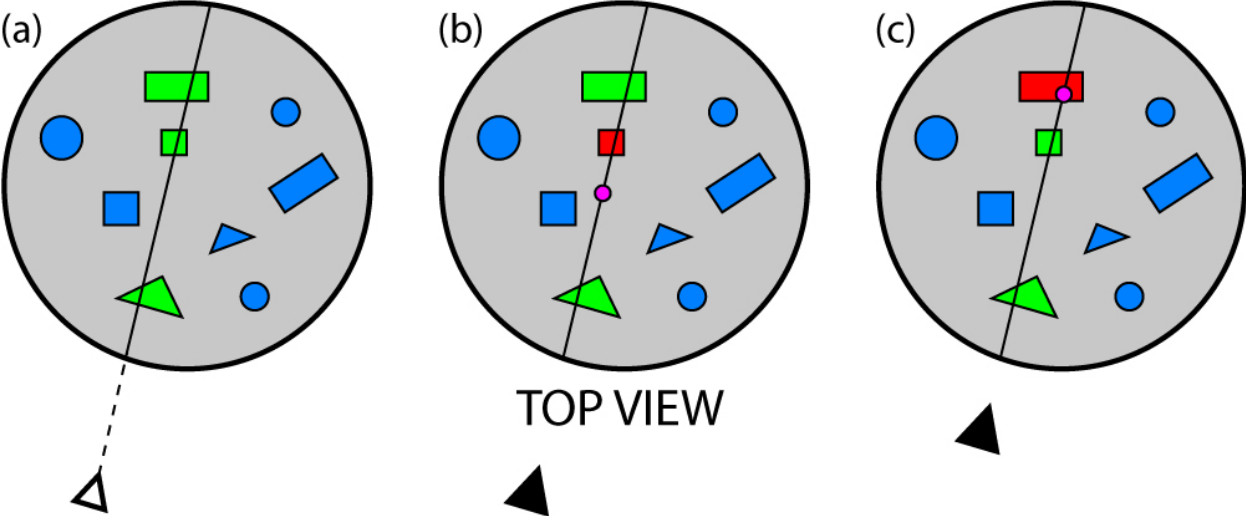
\includegraphics[width=\textwidth]{figures/ch2/lockRay}
			\caption{\emph{Lock Ray}. (a) Première phase : \emph{raycasting} classique. (b) Après pression du bouton du périphérique, un marqueur de profondeur apparaît. (c) L'utilisateur le déplace avec sa main, et sélectionne en relâchant le bouton.}
			\label{fig:lockRay}
		\end{subfigure}
		~
		\begin{subfigure}[t]{\rayWidth}
			\centering
			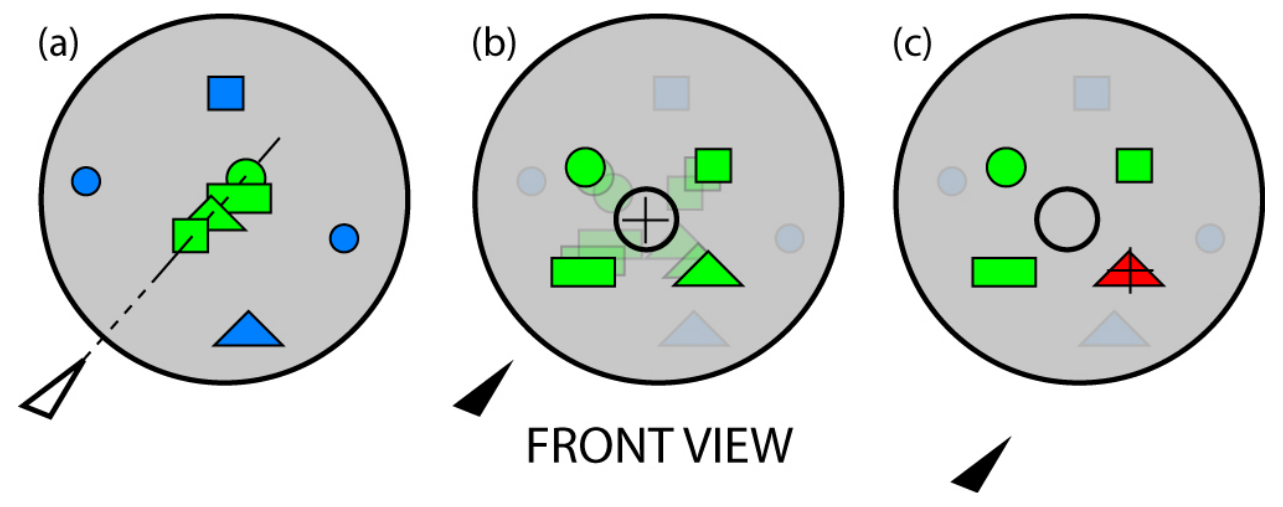
\includegraphics[width=\textwidth]{figures/ch2/flowerRay}
			\caption{\emph{Flower Ray}. (a) Toutes les cibles croisées par le rayon sont en vert. (b) Sur une pression de bouton, elles s'épanouissent en un menu de sélection autour d'un curseur qui apparaît alors. (c) L'utilisateur pointe près de la cible et relâche le bouton pour la sélectionner.}
			\label{fig:flowerRay}
		\end{subfigure}
		~
		\begin{subfigure}[t]{\rayWidth}
			\centering
			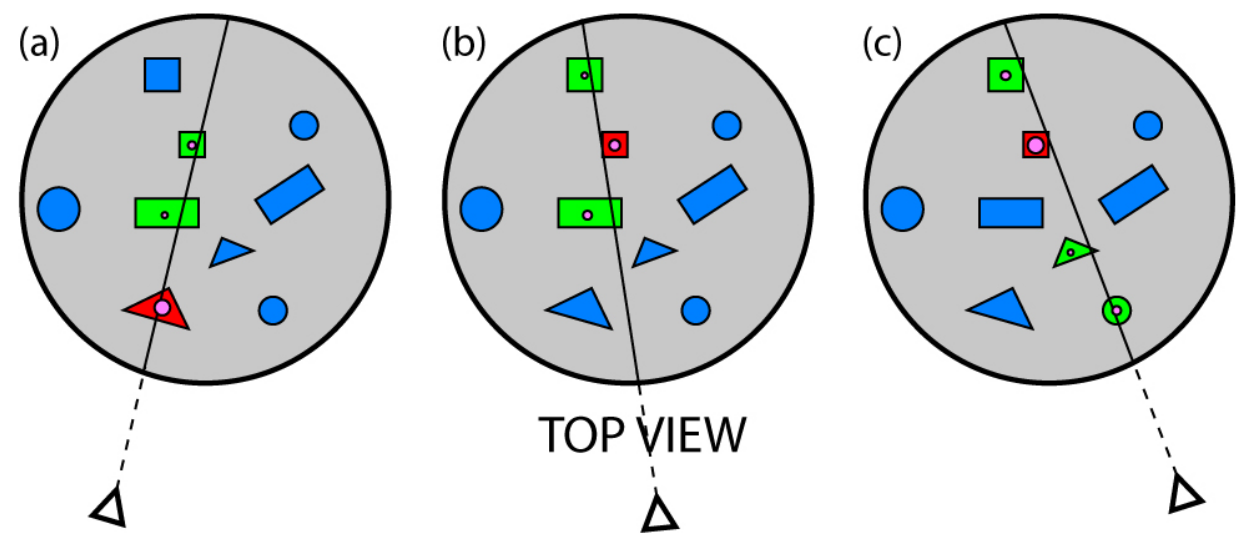
\includegraphics[width=\textwidth]{figures/ch2/smartRay}
			\caption{\emph{Smart Ray}. Sélection du carré. (a) Les poids des cibles dépendent de leur distance au rayon (illustrés par des sphères dans les cibles). La cible de poids maximal peut être sélectionnée. (b,c) Le rayon peut être repositionné pour augmenter le poids de la cible visée.}
			\label{fig:smartRay}
		\end{subfigure}
		\caption[Lancer de rayon avec désambiguïsation]{Techniques de lancer de rayon avec désambiguïsation. Crédit : \cite{grossman2006design}.}
		\label{fig:depthLockFlowerSmartRays}
	\end{figure}
	
	\subsubsection{\emph{Lock Ray}}
	Le \emph{Lock Ray}~\cite{grossman2006design} fonctionne de la même façon que le \emph{Depth Ray}, si ce n'est qu'une fois que le rayon est positionné, il est \emph{verrouillé} --- d'où le nom --- afin de permettre à l'utilisateur de déplacer le marqueur de profondeur sans avoir à craindre de faire bouger le rayon par accident.
	
	\subsubsection{\emph{Flower Ray}}
	Comme le \emph{Lock Ray}, le \emph{Flower Ray}~\cite{grossman2006design} fonctionne avec deux phases distinctes. Dans la première, l'utilisateur place son rayon dans la position et l'orientation qu'il désire ; puis, il le fixe, et les objets croisés par le rayon \og s'épanouissent \fg{}  --- tout autour d'un curseur ponctuel, comme les pétales d'une fleur autour de son pistil, ainsi que l'illustre la figure~\ref{fig:flowerRay}. Dans le menu \og floral \fg{} les objets sont disposés par ordre de profondeur croissante dans le sens horaire, avec le plus proche en haut à droite.
		
	\subsubsection{\emph{Smart Ray}}
	Par définition, un rayon contient une infinité de points. Toutefois, si deux sont sécants, alors ils n'ont qu'un seul point en commun. Il donc possible d'utilier deux rayons pour effectuer une sélection par \emph{raycasting} sans aucune ambiguïté. Toutefois, cela nécessite deux périphériques de saisie et cela occupe les deux mains de l'utilisateur.
	
	Le \emph{Smart Ray}~\cite{grossman2006design} propose donc de faire cela avec deux rayons issus du même périphérique, mais mesurés à deux instant différents, selon un principe proche de celui du \emph{Shadow Cone}~\cite{steed20043d}. Chaque objet se voit attribuer un \og poids \fg{} qui croît d'autant plus que le rayon est proche de son centre, ou décroît d'autant plus qu'il en est loin, continuellement. L'objet dont le poids est le plus élevé peut être sélectionné, comme l'illustre la figure~\ref{fig:smartRay}.
	
	\subsubsection{Motivations}
	Grossman \emph{et al.}~\cite{grossman2006design} notent que les techniques présentées ci-dessus ont chacune des avantages et des inconvénients. Le \emph{Depth Ray} unifie les phases de sélection et de désambiguïsation, ce qui peut faire gagner du temps mais aussi causer des perturbations entre les phases. Le \emph{Lock Ray} sépare les phases explicitement, mais désambiguïse avec un menu linéaire. Le \emph{Flower Ray} propose un menu radial, théoriquement plus rapide, mais les utilisateurs doivent suivre l'animation pour ne pas perdre leur cible entre les deux phases. Enfin, le \emph{Smart Ray} fournit un mode de désambiguïsation implicite et possiblement plus fluide, mais potentiellement source de frustration s'il échoue à prédire correctement l'intention de l'utilisateur, comme toujours avec les techniques prédictives.
	
	\subsubsection{Évaluations}
	Avec ces mérites respectifs en tête, Grossman \emph{et al.} ont évalué ces quatre techniques dans un environnement dense, afin de rendre la désambiguïsation absolument nécessaire. De fait, la sélection par \emph{raycasting} classique est impossible, et donc ne fut pas évaluée ici. La technique de base considérée est donc le curseur ponctuel.

	\paragraph{Temps de sélection.}
	
	Les temps de sélection mesurés par les auteurs pour les différentes techniques sont représentés sur la figure~\ref{fig:rayTimes}.
	
	\begin{figure}[!htbp]
		\begin{subfigure}[t]{0.42\textwidth}
			\centering
			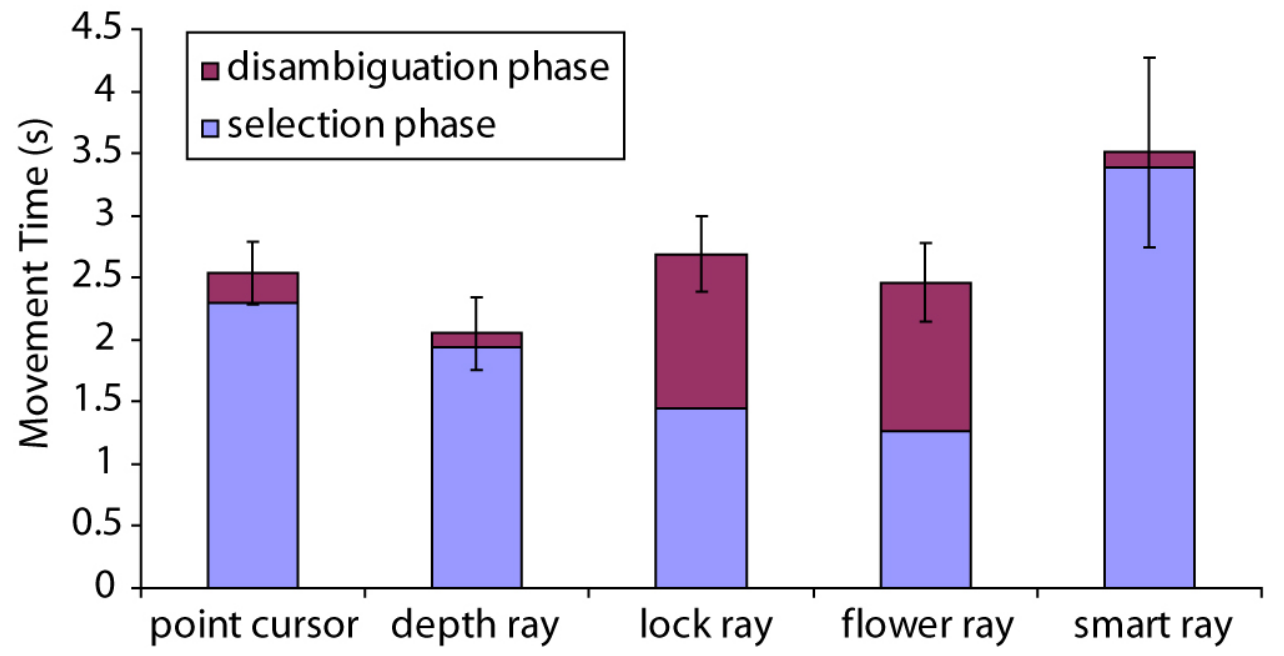
\includegraphics[width=\textwidth]{figures/ch2/rayTimes}
			\caption{Techniques de \emph{raycasting} avec désambiguïsation en environnement dense. Seul le \emph{Depth Ray} se montre plus performant que le curseur ponctuel.}
			\label{fig:rayTimes}
		\end{subfigure}
		~
		\begin{subfigure}[t]{0.56\textwidth}
			\centering
			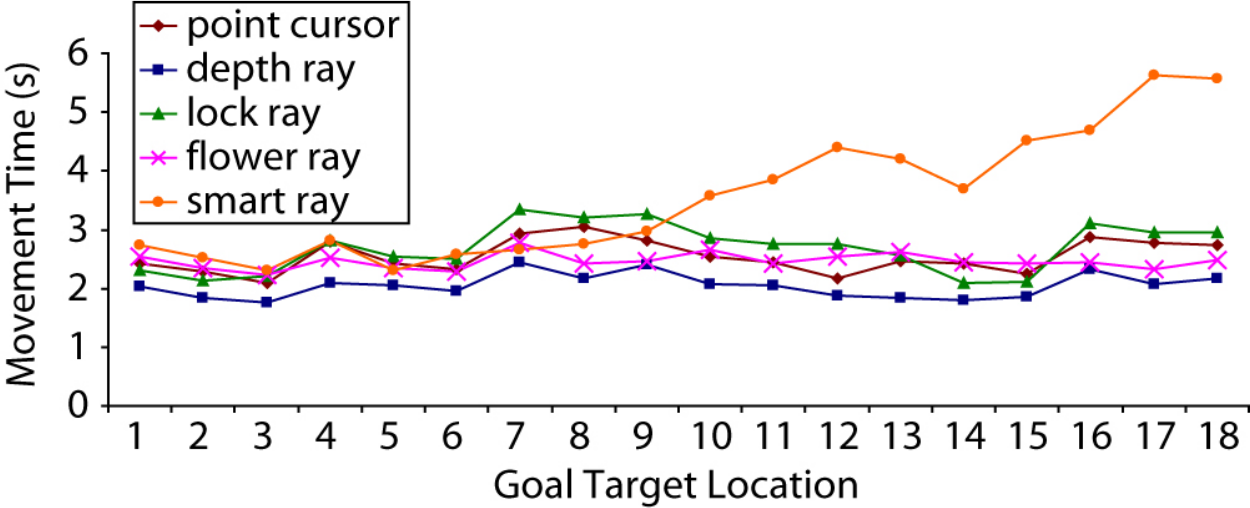
\includegraphics[width=\textwidth]{figures/ch2/smartRayLocation}
			\caption{Pour les cibles à gauche, le \emph{Smart Ray} fournit de bons résultats, pas pour les cibles à droite. Les sujets de l'évaluation étaient droitiers, donc le rayon venait de la droite, et rencontrait beaucoup d'obstacles.}
			\label{fig:smartRayLocation}
		\end{subfigure}
		\caption[Performances du \emph{raycasting} avec désambiguïsation]{Performances du \emph{raycasting} avec désambiguïsation. Crédit : \cite{grossman2006design}.}
		\label{fig:rayPerf}
	\end{figure}

	Le premier constat est que le curseur ponctuel offre de très bonnes performances par rapport aux techniques de \emph{raycasting}, ce qui peut surprendre compte tenu des performances généralement supérieures de ces dernières~\cite{bowman2001testbed}. Mais le niveau d'occultation avec de nombreux distracteurs est tel que les performances de cette classe de techniques chutent. Toutefois, le \emph{Depth Ray} fournit de très bons résultats, meilleurs que ceux du curseur ponctuel. Il profite selon toute probabilité de l'intégration des phases de sélection et de désambiguïsation. Grossman \emph{et al.} remarquent au passage que le temps de désambiguïsation du \emph{Flower Ray} est relativement constant en fonction de l'emplacement de la cible, alors que celui du \emph{Lock Ray} varie beaucoup ; sans doute le menu radial du premier a-t-il un effet lisseur sur cette valeur.

	\paragraph{Performances selon l'emplacement de la cible.}
	Les performances du \emph{Smart Ray} paraissent décevantes. Un examen plus poussé des résultats montre toutefois une forte interaction entre le temps de sélection et l'emplacement de la cible avec cette technique (voir la figure~\ref{fig:smartRayLocation}). Pour les cibles situées à droite, les performances s'effondrent, car le rayon part également de la droite (tous les sujets étant droitiers) donc rencontre beaucoup d'obstacles. Dans ces conditions, l'heuristique de prédiction du \emph{Smart Ray} échoue plus souvent.

	Ces mauvais résultats du \emph{Smart Ray} sont toutefois à nuancer, puisque les sujets avaient pour instruction de ne pas bouger leurs pieds ; s'ils avaient pu se déplacer, les résultats auraient probablement été meilleurs, à condition que leur temps de déplacement ne soit pas assez long pour annuler le bénéfice du déplacement.
	
	\paragraph{Distance parcourue par le périphérique.}
	Les auteurs ont par ailleurs mesuré la distance parcourue par le périphérique de pointage au cours d'une tâche de sélection, pour chaque technique évaluée. C'est un résultat important car il est déterminant pour la fatigue ressentie par un utilisateur sur une durée significative. Ici encore, le \emph{Smart Ray} déçoit, tandis que les autres techniques permettent de réduire la distance à parcourir par rapport au curseur ponctuel, comme l'illustre la figure~\ref{fig:rayFootprint}.
	
	\begin{SCfigure}[50][htbp]
		\centering
		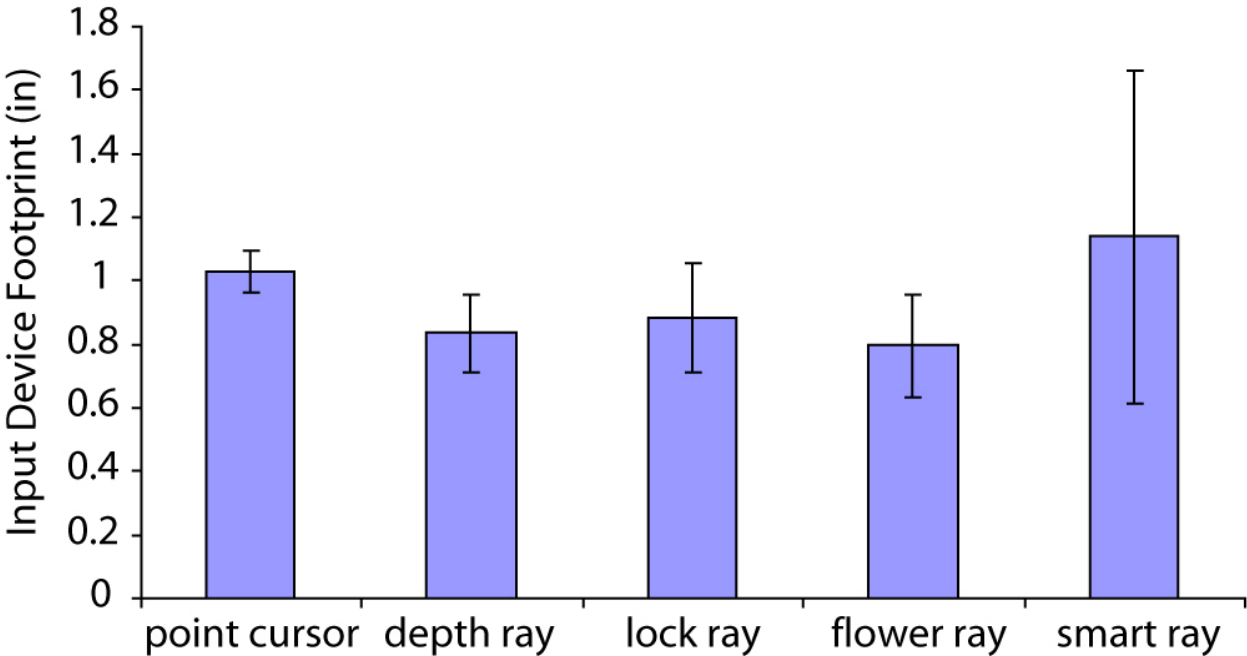
\includegraphics[width=0.46\textwidth]{figures/ch2/rayFootprint}
		\caption[\emph{Raycasting} et désambiguïsation -- distance parcourue par le périphérique]{Distance parcourue par le périphérique de pointage avec les techniques de \emph{raycasting} évaluées. Les \emph{Depth, Lock} et \emph{Flower Rays} font mieux que le curseur ponctuel, au contraire du \emph{Smart Ray} qui affiche en sus un écart-type considérable. Crédit : \cite{grossman2006design}.}
		\label{fig:rayFootprint}
	\end{SCfigure}
	
	Là encore on peut s'interroger sur la solidité des distances mesurées sur \emph{Smart Ray} attendu que dans un contexte \og réel \fg{} les utilisateurs seraient libres de se déplacer. Naturellement, la quantité de mouvement absolue du pointeur pourrait s'en trouver accrue, mais sa quantité de mouvement relatif à l'utilisateur pourrait diminuer. Il resterait à déterminer s'il est plus fatigant de bouger beaucoup son bras, ou un peu son corps et un peu son bras. Cette question est à notre connaissance ouverte.
	
	\paragraph{Taux d'erreurs.}
	Enfin, Grossman \emph{et al.} rapportent que les taux d'erreurs sont avantageux avec ces techniques de \emph{raycasting} avec désambiguïsation, comme le détaille la table~\ref{tab:rayErrors}.
	
%	\newcommand{\newrow}{\bigstrut[t] \\ \hline}
	\begin{table}[htbp]
	\centering
	\begin{tabular}{c c}
		Type de curseur			& Taux d'erreurs \bigstrut[b] \\ \hline
		Curseur ponctuel		& 20,7~\%{} \bigstrut[t] \\
		\emph{Depth Ray}		& 13,3~\%{} \\
		\emph{Lock Ray}			& 11,1~\%{} \\
		\emph{Flower Ray}		& 10,9~\%{} \\
		\emph{Smart Ray}		& 10,4~\%{} \\
	\end{tabular}
	\caption[Taux d'erreurs pour les techniques de \emph{raycasting} avec désambiguïsation]{Taux d'erreurs pour les techniques de \emph{raycasting} avec désambiguïsation. Données tirées de~\cite{grossman2006design}.}
	\label{tab:rayErrors}
	\end{table}
	
	\subsubsection{Conclusion}
	L'étude de Grossman \emph{et al.}~\cite{grossman2006design} montre qu'en environnement dense, la sélection par \emph{raycasting} pur est moins efficace qu'un curseur ponctuel, voire impossible, mais que des méthodes de désambiguïsation peuvent permettre d'atteindre de meilleures performances. Dans une certaine mesure, on peut en effet améliorer les temps de sélection, mais les bénéfices sur les taux d'erreurs sont encore plus importants.
	
	Parmi les techniques évaluées ici, le \emph{Depth Ray} se distingue des autres avec de très bons temps de sélection, et un taux d'erreurs légèrement plus élevé que ceux des autres techniques avancées, mais tout de même nettement inférieur à ce qu'on obtient avec un curseur ponctuel. Toutefois, le \emph{Depth Ray} souffre d'un léger inconvénient, puisqu'il nécessite un périphérique de pointage permettant de capturer non seulement son orientation, mais également sa position, c'est-à-dire qu'un simple gyroscope est insuffisant. Ce n'est pas nécessairement le cas du \emph{Lock Ray} ou du \emph{Flower Ray}, par exemple. Néanmoins, la profondeur pourrait éventuellement être gérée par un contrôle additionnel sur le périphérique de pointage, tel qu'une molette, par exemple.
	
	Ce qui est potentiellement plus gênant avec le \emph{Depth Ray} est le couplage des phases de pré-sélection et de désambiguïsation. Si ce couplage est bénéfique ici, on peut en douter dans le cas de cibles mobiles, où il faudrait constamment réajuster l'orientation du rayon pour continuer à \og capturer \fg{} la cible, tout en avançant ou reculant le périphérique pour placer le marqueur de profondeur au bon endroit. Nous supposons que pour des cibles petites et/ou rapides, le \emph{Depth Ray} serait très difficile à utiliser, là où un \emph{Lock/Flower Ray} pourrait fournir des performances satisfaisantes, à condition peut-être d'utiliser un cône un peu large au lieu d'un rayon cylindrique --- en réalité, ces techniques furent mises en \oe{}uvre par Grossman \emph{et al.} avec des cônes de 2\textdegree{} d'angle, même si ce n'était pas indiqué par le rendu graphique.
	
	Si le \emph{Smart Ray} fournit ici d'assez mauvais résultats, il serait intéressant de le réévaluer dans ce contexte, car d'une part, il souffrirait peut-être moins de l'occultation de la cible si elle était mobile, et d'autre part, il ne serait peut-être plus nécessaire de bouger le rayon pour lever l'ambiguïté, puisqu'en suivant la cible, son poids augmenterait continuellement, tandis que les poids des distracteurs seraient susceptibles de baisser assez rapidement --- à moins que ceux-ci ne se déplacent de façon corrélée à la cible, en étant toujours touchés par le rayon, ce qui est assez improbable sur une durée de plusieurs secondes dans la plupart des cas.
	
	Ainsi, les inconvénients principaux de cette technique, à savoir la distance parcourue par le périphérique et l'occultation pourraient être atténués, tandis que l'heuristique de prédiction pourrait \emph{mieux} fonctionner qu'avec des cibles statiques. Nous verrons plus loin que la technique \emph{IntenSelect}~\cite{de2005intenselect} fonctionne à peu près sur ce principe, de même que \emph{Hook}~\cite{ortega2013hook}, qui fait cependant usage d'un curseur ponctuel.
	
	Ajoutons enfin que le \emph{Smart Ray} pourrait être adapté pour utiliser, en plus du rayon projeté par le périphérique de pointage, un cône (relativement étroit) orienté selon la direction du regard de l'utilisateur. Ainsi, les objets dont les poids augmenteraient seraient ceux situés à la fois dans le cône de vision de l'utilisateur et proches du rayon.

	\subsection{Sélection en cascade, grossière, puis fine}
	Les techniques de cette catégorie divisent la sélection en deux phases (ou plus). Premièrement, une portion de l'espace visuel est sélectionnée. Cette première phase étant grossière, elle n'a pas besoin d'être précise, et peut être très rapide. Par exemple, avec un simple périphérique de pointage, tel qu'une souris, un ratio contrôle/affichage (\emph{control/display, C/D}) très faible peut être utilisé. Le curseur (ou autre medium de sélection) peut ainsi se placer très rapidement sur la zone d'intérêt, mais n'a pas besoin d'être précisément sur la cible pour délencher la deuxième phase : la sélection (plus) fine. Dans celle-ci, l'utilisateur sélectionne la cible elle-même, par exemple à l'aide d'un ratio C/D plus élevé, ou bien affine encore l'espace de sélection, jusqu'à ce qu'une phase finale permette la sélection effective de la cible.
	 
	Du point de vue de la loi de Fitts, au cours d'une phase grossière, la cible bénéficie d'une largeur accrue (car c'est toute une zone autour de la cible qui est visée) tandis que la phase finale offre une distance réduite, puisque le curseur se trouve déjà près de la cible. Quoiqu'il y ait probablement un certain \og coût cognitif \fg{} lié au basculement d'une phase à l'autre, et en tout cas un coût temporel associé à la pression d'un bouton ou à toute autre action permettant de passer à la phase suivante, les techniques de sélection en cascade peuvent améliorer significativement les performances de sélection, même pour les tâches dont l'indice de difficulté est élevé~\cite{kopper2011rapid}.
	
	La sélection en cascade revient, en substance, à préférer une série de tâches très rapides et faciles à une seule tâche nécessitant une précision élevée, prenant du temps et pouvant être source d'erreur plus ou moins fréquentes. Observons que la sélection en cascade, du fait de la réduction du taux d'erreurs qu'elle permet, présente un intérêt particulier pour les tâches critiques, celles pour lesquelles une erreur peut avoir des conséquences graves.
	
	\subsubsection{Utilisation du regard}
	Une estimation de la direction du regard de l'utilisateur peut être utilisée soit pour sélectionner directement la cible (ce qui peut nécessiter beaucoup de précision, quand la cible est petite) soit pour sélectionner une zone d'intérêt, dans la phase grossière d'une sélection en cascade. C'est généralement dans cette seconde fonction que l'on trouve cette technique, selon le principe \og le regard suggère, le toucher confirme \fg{}~\cite{stellmach2012look}.

	L'estimation de la direction du regard d'autrui faite par un individu est basée sur la combinaison de la position de la tête de la personne observée, de l'orientation de sa tête, et de l'orientation de ses yeux~\cite{langton2004influence}, mais elle est fortement biaisée par l'orientation de la tête~\cite{wollaston1824apparent}.
	
	Sur l'hypothèse que l'estimation de la direction du regard faite instinctivement par les êtres humains se base sur une méthode efficace, on peut en déduire qu'une méthode artificielle devrait procéder de la même façon, c'est-à-dire en estimant la position et la direction de la tête d'une part, et la direction des yeux de l'autre. Murphy Chutorian et Trivedi~\cite{murphy2009head} proposent une taxinomie et un inventaire détaillés des techniques d'estimation de la \emph{pose}\footnote{C'est-à-dire de la position \emph{et} de l'orientation.} de la tête. Ces techniques sont toutefois destinées à traiter des données vidéo brutes.
	
	Or, dans le cas qui nous intéressent, il est généralement possible d'installer des marqueurs sur la tête d'un utilisateur pour connaître plus précisément sa \emph{pose}, en s'appuyant également sur des caméras de \emph{tracking}, comme par exemple les systèmes d'Advanced Realtime Tracking\footnotemark{}. Outre sa précision, ce système est autrement plus robuste que les techniques sans marqueurs.
	
	\footnotetext{Des réseaux de caméras infrarouge permettant d'obtenir les positions précises d'un ensemble de marqueurs, donc l'orientation de l'objet sur lequel les marqueurs sont posés --- objet pouvant éventuellement être la tête d'un utilisateur.
	\url{http://www.ar-tracking.com/products/tracking-systems/arttrack-system/arttrack5}}
	
	Comme le rappellent Zhai \emph{et al.}~\cite{zhai1999manual}, l'utilisation des yeux comme entrée dans un système informatique fait l'objet de recherches depuis longtemps~\cite{levine1981eye, bolt1982eyes, ware1987evaluation, jacob1990you}. Ils remarquent également que la fovéa, (la zone centrale de la macula, la zone de la rétine où la vision des détails est la plus précise) avec son angle de 1\textdegree{}, est trop grossière pour les cibles les plus petites, surtout compte tenu des mouvements aléatoire constamment effectués par les yeux~\cite{monden2005evaluation, vspakov2011comparison}. Dans une certaine mesure, ces derniers peuvent être filtrés, mais cela ne règle que partiellement le problème~\cite{zhang2008improving}.
	
	Par ailleurs, il peut être très déroutant pour un utilisateur de \og charger \fg{} un canal sensoriel, habituellement passif\footnotemark{}, d'une fonction de manipulation plus généralement dévolue à une extrémité ou un membre.
	
	\footnotetext{Remarquons cependant que le regard, quand il est contrôlé de façon délibérée, peut être utilisé pour communiquer, par exemple lorsqu'une personne en invite une autre, oralement, à regarder quelque chose qu'elle désigne du regard. Lever les yeux au ciel peut communiquer de l'agacement ou du dédain, etc.}
	
	Dès lors, il serait tentant de rejeter cette technique, et \emph{a fortiori} l'estimation de la \emph{pose} de la tête ne tenant pas compte des yeux, puisque c'est forcément beaucoup moins précis. Mais ce serait faire fi un peu trop rapidement des avantages du suivi des yeux, et en particulier de sa rapidité inégalée. Certes, il ne peut suffire à lui seul à sélectionner un objet d'indice de difficulté élevé ; il n'est pas inutile pour autant, loin s'en faut.

	En effet, des études ont en effet montré que le regard permettait de faire mieux que les périphériques de saisie traditionnels pour des tâches de sélection~\cite{stellmach2012look, ware1987evaluation, smith2000hand, bieg2010eye}.
	
	\paragraph{Suivi des yeux : une tâche ardue.}

	Cependant, le suivi des yeux présente en pratique des difficultés qui peuvent être considérables, dont au moins les suivantes :
	
	\begin{itemize}
		\item Les performances peuvent dépendre de la couleur des yeux ;
		\item Le suivi des yeux ne fonctionne pas toujours bien en environnement sombre, par exemple dans un CAVE ;
		\item Les lunettes peuvent nuire aux performances du système ;
		\item Les lunettes stéréoscopiques, en particulier, occultent partiellement les yeux pour les \emph{trackers} oculaires, et réduisent la luminosité du blanc des yeux.
	\end{itemize}

	Par conséquent, l'utilisation de suivi des yeux se montre souvent difficile à mettre en œuvre, quoique les progrès techniques puissent, dans un futur proche, pallier au moins partiellement ces difficultés.
	
	Du reste, même quand le suivi des yeux est impossible et seule la tête peut être prise en compte, les informations captées demeurent précieuses. En effet, 40~\%{} à 70~\%{} de l'orientation du regard est déterminée par la rotation de la tête, tandis que les 60~\%{} à 30~\%{} restants (respectivement) dépendent des mouvements oculaires~\cite{gauthier1991short}. On peut donc, le plus souvent, obtenir une bonne estimation de la direction du regard en se fondant uniquement sur l'orientation de la tête.
	
	\subsubsection{\emph{Look \&{} Touch}}
	Stellmach \emph{et al.}~\cite{stellmach2012look} ont développé et évalué plusieurs techniques fondées sur le principe de la sélection en cascade avec une phase grossière dirigée par le regard, et une phase fine s'appuyant sur un périphérique doté d'un écran tactile, tel qu'un \emph{smartphone}.
	
	\begin{enumerate}
		\item \textbf{\emph{Gaze-directed cursor} :} Ce mode très simple peut à peine être considéré comme une cascade : l'utilisateur suit sa cible des yeux, puis appuie sur un écran tactile et le relâche pour effectuer la sélection. Voir la figure~\ref{fig:lookandtouch}, à gauche.
		\item \textbf{\emph{MAGIC touch} absolue :} Cette technique est analogue à la précédente, mais le curseur peut être déplacé en fonction de la position absolue du doigt de l'utilisateur sur son écran tactile. Voir la figure~\ref{fig:lookandtouch}, deuxième vignette.
		\item \textbf{\emph{MAGIC touch} relative :} Cette technique est identique à la précédente, mais le curseur positionnement du curseur dépend des mouvements relatifs du doigt de l'utilisateur par rapport à son point de départ. Voir la figure~\ref{fig:lookandtouch}, troisième vignette.
		\item \textbf{\emph{MAGIC tab} :} Cette technique demeure similaire aux précédentes, mais le curseur ne bouge pas ; en revanche, l'utilisateur peut parcourir les objets comme dans un menu, en faisant glisser son doigt. Ce procédé s'inspire de la touche \emph{tabulation} d'un clavier. Voir la figure~\ref{fig:lookandtouch}, à droite.
		\item \textbf{\emph{Gaze-supported Expanded Target Selection} asservie au regard :} Le regard contrôle une lentille de zoom, inactive par défaut, mais activée en appuyant sur l'écran tactile. Une nouvelle pression permet de sélectionner la cible, tandis qu'un geste de glissement vertical permet d'ajuster le niveau de zoom. Cette technique est illustrée par la figure~\ref{fig:lookandtouch2}, à gauche et au milieu.
		\item \textbf{\emph{Gaze-supported Expanded Target Selection} semi-fixe :} Contrairement à la technique précédente, la lentille cesse de bouger une fois activée, et l'utilisateur déplace le curseur au sein de la zone de zoom à l'aide de son regard, avant d'activer la sélection avec son écran tactile. Si son regard quitte la zone de zoom, alors la lentille se déplace. Voir la figure~\ref{fig:lookandtouch2}, vignettes de gauche et de droite.
	\end{enumerate}
	
	\begin{figure}[!htbp]
		\centering
		\begin{subfigure}[t]{\textwidth}
			\centering
			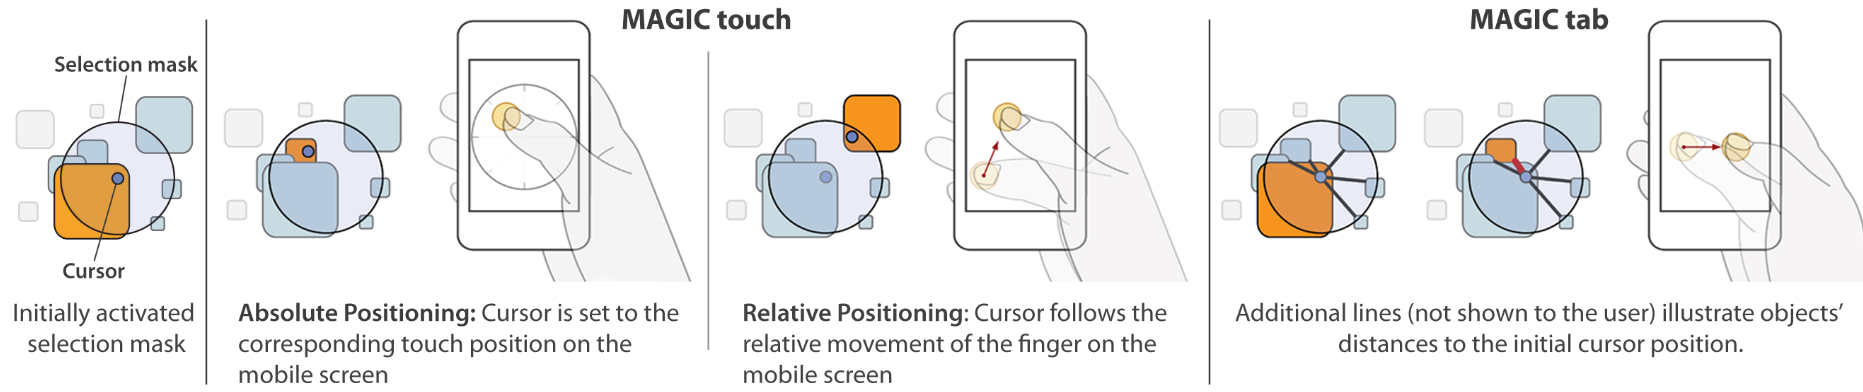
\includegraphics[width=\textwidth]{figures/ch2/lookandtouch}
			\caption[\emph{Look \&{} Touch -- principe}]{Fonctionnement des quatre premiers modes de sélection en cascade de la famille \emph{Look \&{} Touch}.}
			\label{fig:lookandtouch}
		\end{subfigure}
		~
		\begin{subfigure}[t]{\textwidth}
			\centering
			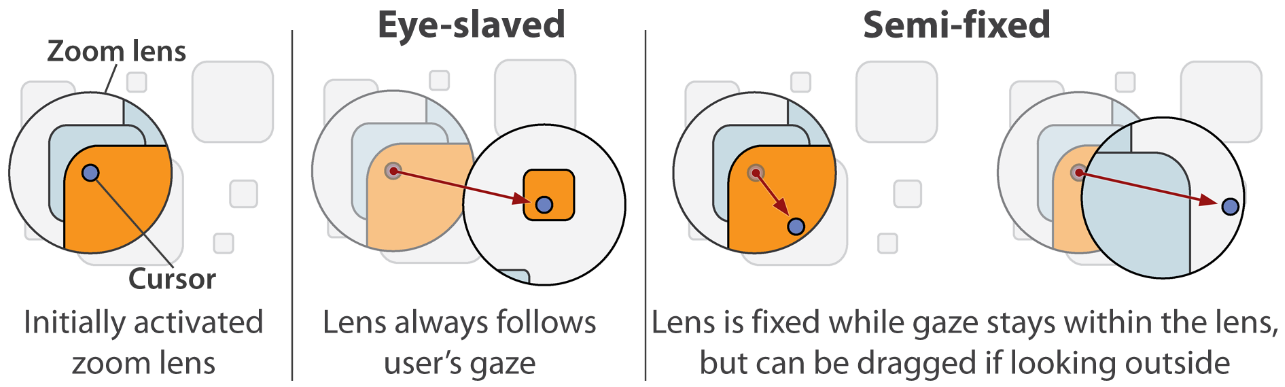
\includegraphics[width=0.8\textwidth]{figures/ch2/lookandtouch2}
			\caption[\emph{Look \&{} Touch -- principe II}]{Fonctionnement des deux derniers modes de sélection en cascade de la famille \emph{Look \&{} Touch}.}
			\label{fig:lookandtouch2}
		\end{subfigure}
		\caption[\emph{Look \&{} Touch} -- principe]{\emph{Look \&{} Touch} -- principe. Crédit : \cite{stellmach2012look}.}
		\label{lookAndTouchPrinciple}
	\end{figure}
	
	\paragraph{De bons résultats, sans vainqueur clair.}
	Stellmach \emph{et al.} ont évalué les variantes de \emph{Look \&{} Touch} sus-citées dans trois blocs de tâches : T1, avec des objets disjoints sur une grille 2D ; T2, avec une ligne d'objets 2D se chevauchant ; et T3, avec des objets 2D de tailles diverses se chevauchant.
	
	Diverses tailles et distances ont également été testées. Les temps de sélection et les taux d'erreurs ont été mesurés ; ils sont rapportés sur la figure~\ref{fig:latRes}. Si le \emph{Gaze-directed cursor} montre rapidement ses limites, les autres techniques fournissent de bonnes performances dans la plupart des cas, avec peut-être un léger avantage global à la technique \emph{MAGIC tab}. Du moins cette tendance est-elle confirmée par les impressions sujectives recueillies par Stellmach \emph{et al.}, et exposées sur la figure~\ref{fig:latSubj}.

	\begin{figure}[!htbp]
%		\centering
		\begin{subfigure}[t]{\textwidth}
			\centering
			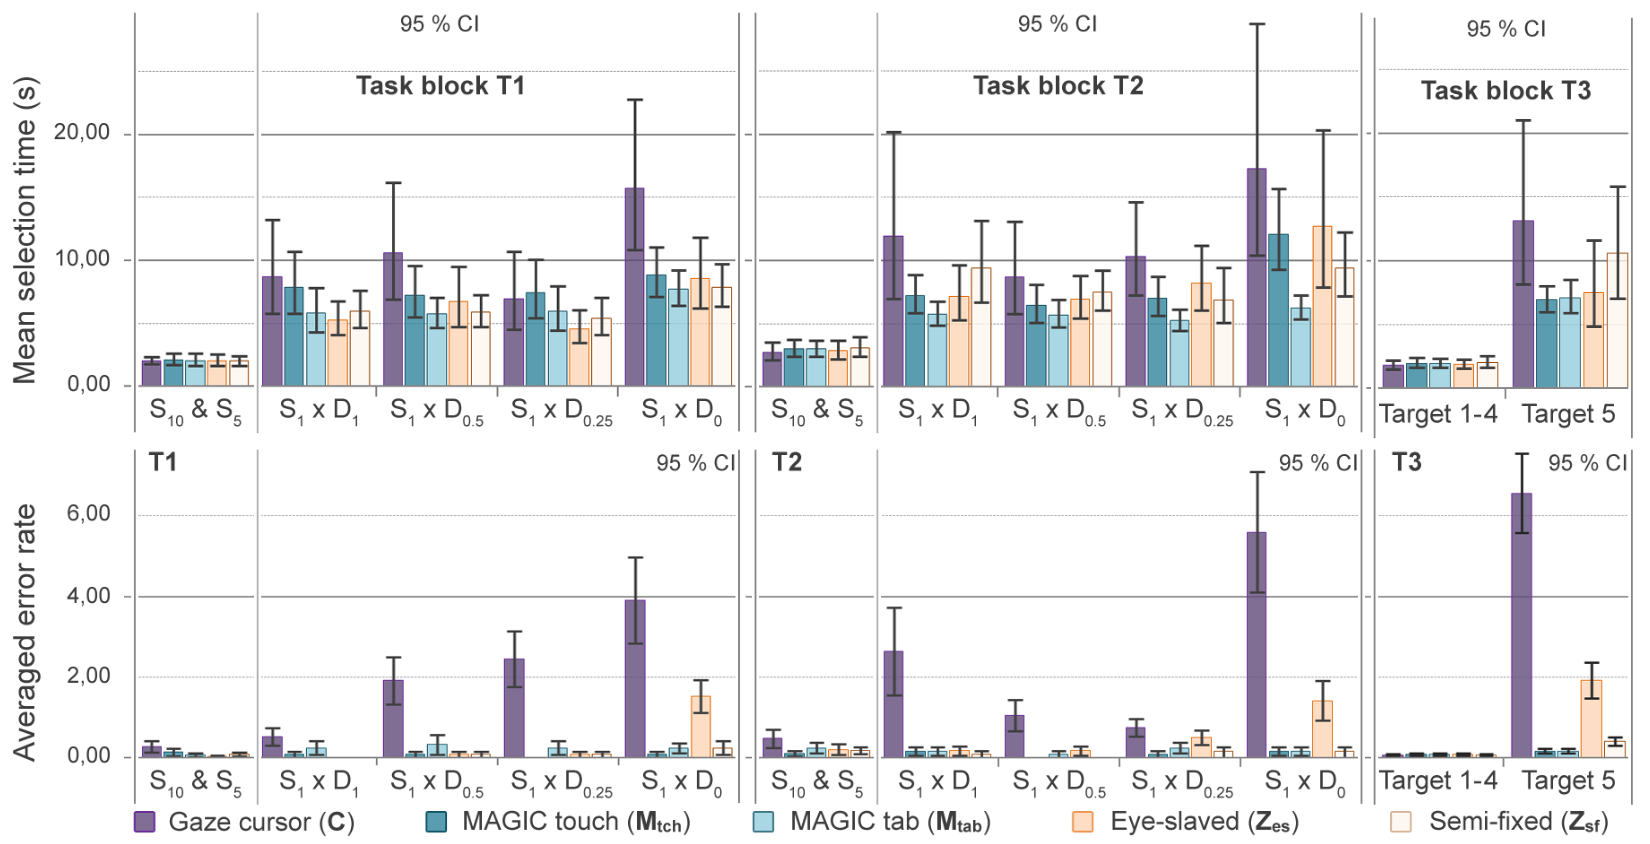
\includegraphics[width=\textwidth]{figures/ch2/latRes}
			\caption[\emph{Look \&{} Touch} -- performances]{Performances. Les temps de sélection sont en haut, et les taux d'erreurs en bas. Les mentions $S_{i}$ et $D_{i}$ indiquent respectivement les différentes tailles et distances.}
			\label{fig:latRes}
		\end{subfigure}
		~
		\begin{subfigure}[t]{\textwidth}
			\centering
			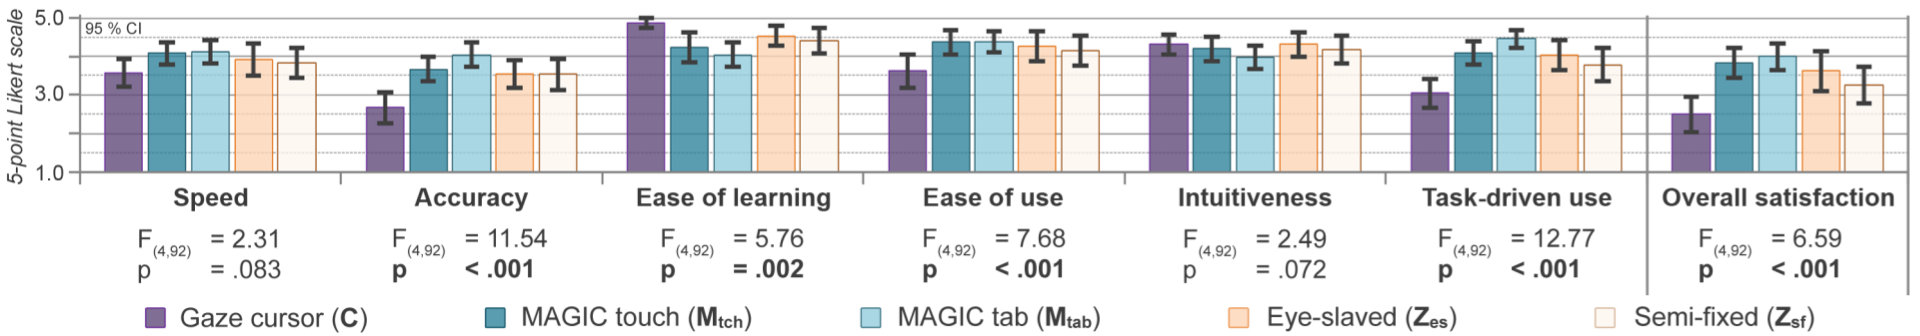
\includegraphics[width=\textwidth]{figures/ch2/latSubj}
			\caption[\emph{Look \&{} Touch} -- impressions subjectives]{Impressions subjectives recueillies par Stellmach \emph{et al.} auprès des sujets de l'évaluation. La technique \emph{MAGIC tab} l'emporte, mais d'une très courte tête.}
			\label{fig:latSubj}
		\end{subfigure}
		\caption[\emph{Look \&{} Touch} -- performances]{\emph{Look \&{} Touch} -- performances et impressions. Crédit : \cite{stellmach2012look}.}
	\end{figure}
	
	\paragraph{\emph{MAGIC tab} et le problème de linéarité.}
	Si, comme l'on vient de le voir, la technique \emph{MAGIC tab} sort légèrement du lot et se hisse en tête des résultats objectifs et subjectifs, elle souffre d'une limitation inhérente à sa nature : le temps de sélection dans la phase fine dépend de façon approximativement linéaire du nombre d'objets à parcourir, puisque l'utilisateur est contraint de faire ce parcours de façon linéaire.
	
	En comparaison, la plupart des processus de sélection sont accompagnés d'une relation logarithmique entre le nombre d'objets et le temps de sélection~\cite{hick1952rate, hyman1953stimulus}. L'on peut donc émettre des doutes sur la robustesse de \emph{MAGIC tab} dans des environnements très denses.
	
	Ajoutons que le comportement de cette technique avec des cibles mobiles pose question, puisque le menu contiendrait des objets n'étant plus nécessairement dans l'espace de pré-sélection au moment où l'utilisateur les parcourt. Cette perte de contexte spatial pourrait, dans le cas de cibles visuellement très proches (ou identiques) rendre la sélection impossible.
	
	\subsubsection{\emph{Sphere-casting refined by QUAD-menu
(SQUAD)}}
	Un exemple typique de méthode de sélection en cascade est la technique \emph{Sphere-casting refined by QUAD-menu
(SQUAD)}~\cite{kopper2011rapid}. Avec SQUAD, l'utilisateur commence par sélectionner un volume contenant sa cible ; puis, il affine progressivement sa sélection en choisissant le sous-ensemble de cibles contenant celle qu'il veut, via un menu à quatre options affichant tous les objets n'ayant pas encore été éliminés ; \emph{in fine}, le dernier objet restant est sélectionné. Aucune des sous-tâches de SQUAD ne nécessite d'être précis. Le fonctionnement de cette technique est illustré par la figure~\ref{fig:squad}.

	\begin{figure}[!htbp]
		\centering
		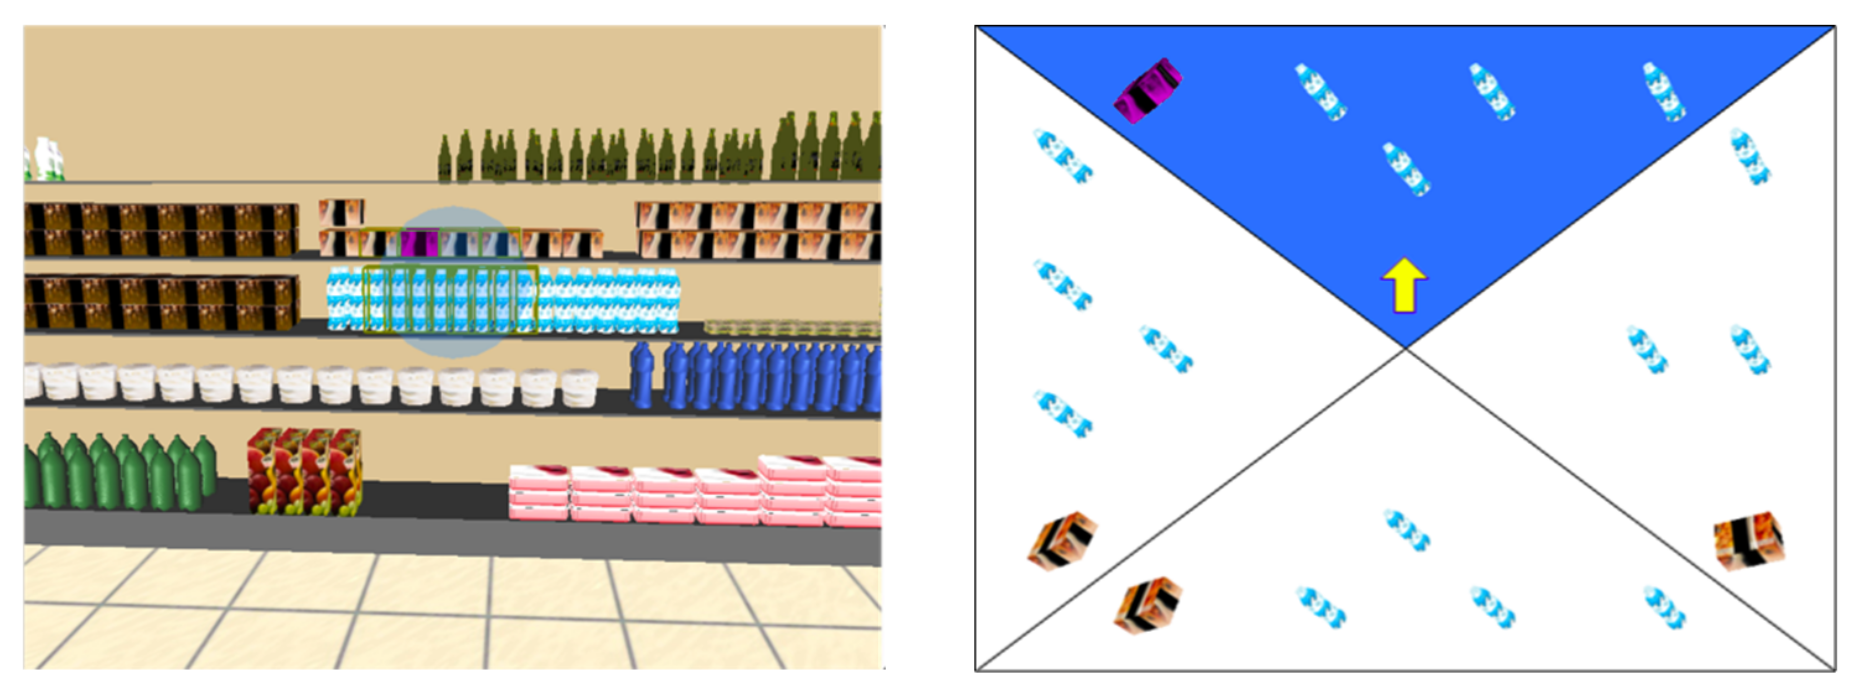
\includegraphics[width=\textwidth]{figures/ch2/squad}
		\caption[Fonctionnement de la technique SQUAD]{SQUAD : à gauche, la première étape de sélection, au cours de laquelle l'utilisateur pré-sélectionne une portion de l'espace à l'aide d'une sphère. À droite, la phase suivante, permettant d'affiner la sélection. Les objets pré-sélectionnés avec la sphère sont uniformément répartis dans quatre quadrants d'un menu, et l'utilisateur n'a plus qu'à choisir le quadrant contenant l'objet qu'il souhaite sélectionner. Les autres quadrants se vident, puis les objets du quadrant sélectionné sont répartis dans les quatre afin de permettre, dans une nouvelle étape, d'affiner encore la sélection. L'opération est répétée jusqu'à ce qu'il n'y ait plus qu'un objet, qui est sélectionné. Crédit : \cite{kopper2011rapid}.}
		\label{fig:squad}
	\end{figure}
	
	Bien que le procédé puisse paraître pénible, il permet d'affiner la sélection jusqu'au dernier élément en $log_{4}(n)$ étapes, où $n$ est le nombre d'objets pré-sélectionnés par la sphère au cours de la première étape. Naturellement, il faut ajouter à cela l'étape de pré-sélection. Au total, la sélection d'un objet parmi 256 se fait en seulement 5 étapes, où chaque étape peut être très rapide.
	
	En pratique, dans~\cite{kopper2011rapid}, SQUAD fut évaluée avec des objets uniformes : des sphères de rayons identiques. Seule la couleur variait, avec du gris pour des distracteurs et du rouge pour la cible à sélectionner, comme on le voit sur la figure~\ref{fig:squad2}. 
	
	\begin{figure}[!htbp]
		\centering
		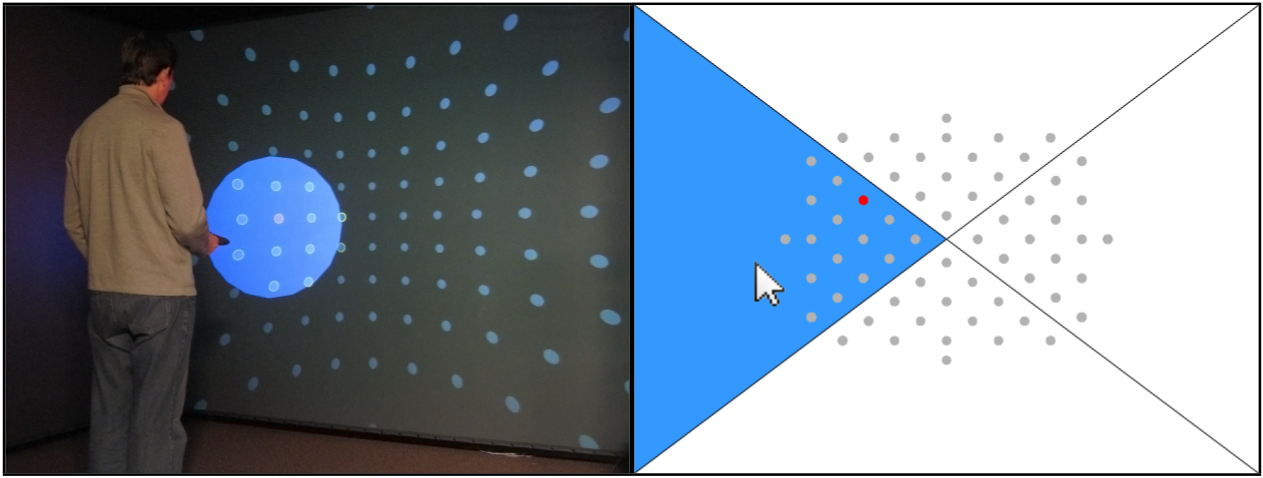
\includegraphics[width=\textwidth]{figures/ch2/squad2}
		\caption[La technique SQUAD -- évaluation]{SQUAD tel qu'évalué dans~\cite{kopper2011rapid}. Dans la première phase (à gauche) les petites sphères sont réparties sur la surface d'une grande sphère invisible centrée sur l'utilisateur, de sorte qu'elles sont toutes à la même distance de lui, afin qu'elles aient toutes une taille apparente égale une fois projetées sur l'écran. La cible à saisir est identifiée par sa couleur rouge. Seule l'orientation du périphérique de pointage était prise en compte dans la première phase, et les sujets avaient pour consigne de maintenir sa position dans une zone déterminée. Crédit : \cite{kopper2011rapid}.}
		\label{fig:squad2}
	\end{figure}
	
	\paragraph{Performances.}
	Les performances de SQUAD, comparée au \emph{raycasting} et en fonction du nombre de distracteurs sont détaillées sur la figure~\ref{fig:squadDensity}. On constate que SQUAD offre de meilleures performances en environnement dense, de moins bonnes en environnement peu dense, et des résultats comparables entre les deux. Les mêmes résultats sont présentés sur la figure~\ref{fig:squadSize}, mais en fonction de la taille des cibles. Comme attendu, les performances de SQUAD sont à peu près constantes tandis que le \emph{raycasting} est d'autant plus performant que les cibles sont grandes. De fait, la technique SQUAD est avantageuse avec de petites cibles, désavantageuses quand elles sont grandes, et à peu près équivalent entre les deux.
	
	\begin{figure}[!htbp]
		\begin{subfigure}[t]{0.49\textwidth}
			\centering
			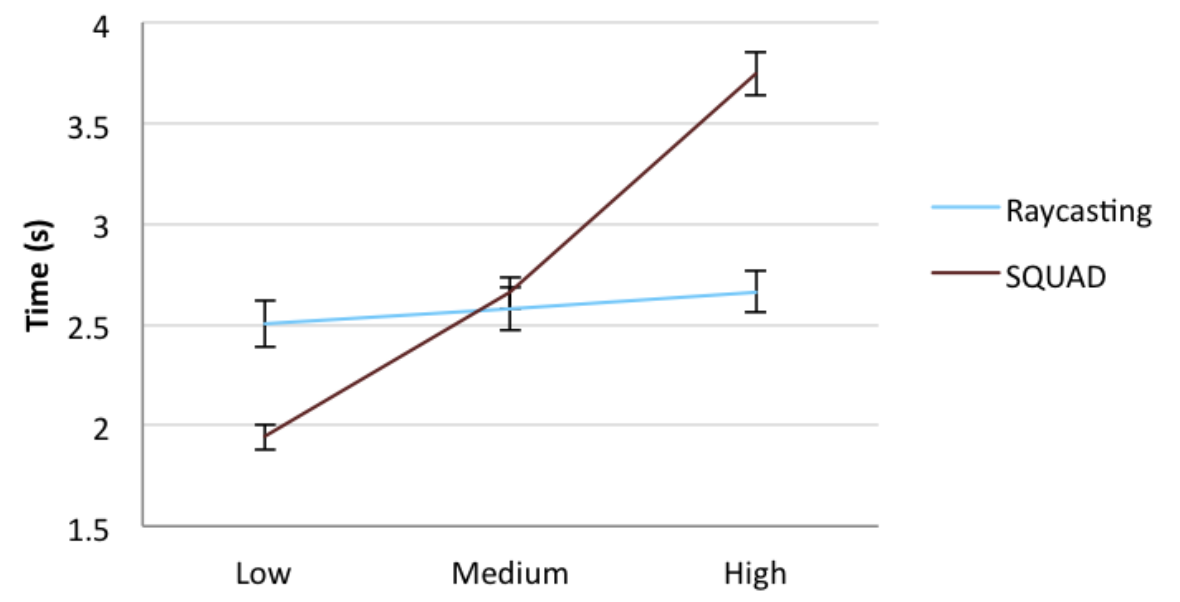
\includegraphics[width=\textwidth]{figures/ch2/squadDensity}
			\caption{Performances de SQUAD en fonction de la densité de distracteurs, comparées avec celle du \emph{raycasting}. Les performances de ce dernier ne sont pas significativement modifiées par la densité, même si une légère corrélation est visible, peut-être due à la recherche visuelle de la cible. Les performances de SQUAD sont fortement affectées, car le nombre d'étapes dépend de la densité. SQUAD brille dans les conditions de faible densité, mais se montre désavantageuse quand les distracteurs sont nombreux.}
			\label{fig:squadDensity}
		\end{subfigure}
		~
		\begin{subfigure}[t]{0.49\textwidth}
			\centering
			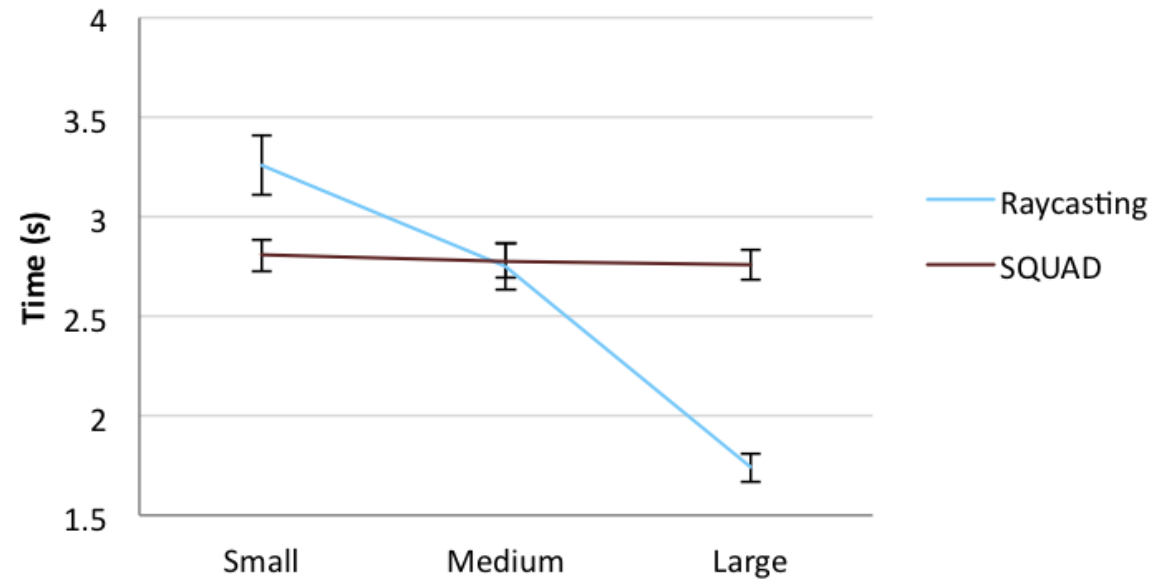
\includegraphics[width=\textwidth]{figures/ch2/squadSize}
			\caption{Performances de SQUAD comparées avec celles du \emph{raycasting}, en fonction de la taille des cibles, avec différentes densités de distracteurs. SQUAD est plus performante à faible densité, et capable de gérer de très petites cibles sans augmentation notable du temps de sélection, ce qui est intéressant pour certaines applications. Avec de grosses cibles, on préférera le \emph{raycasting}, en particulier dans ses formes améliorées.}
			\label{fig:squadSize}
		\end{subfigure}
		\caption[Performances de SQUAD]{Performances de SQUAD. Crédit : \cite{kopper2011rapid}.}
		\label{fig:squadPerf}
	\end{figure}
	
	Un récapitulatif de ces résultats est présenté sur la figure~\ref{fig:squadRecap}. On constate que la technique SQUAD gère très bien les petites cibles, mais voit ses performances chuter avec le nombre de distracteurs. Notons par ailleurs que le taux d'erreurs avec SQUAD était extrêmement faible, avec seulement 0,7~\%{}, ce qui est un atout notable pour cette technique. De fait, si l'on considérait non pas les temps de sélection, mais les temps de sélection normalisés par rapport aux erreurs, l'évaluation serait nettement plus favorable à SQUAD.
	
	\begin{figure}[!htbp]
		\centering
		\includegraphics[width=0.65\textwidth]{figures/ch2/squadRecap}
		\caption[SQUAD -- résultats : taille]{Performances de SQUAD en fonction de la taille de la cible, comparées avec celles du \emph{raycasting}. Les performances de SQUAD ne sont pas significativement modifiées par la taille, même si une légère corrélation négative est visible, peut-être due à la recherche visuelle de la cible quand elle est petite. Les performances du \emph{raycasting} sont fortement affectées, puisqu'une petite cible a un ID bien plus élevé. SQUAD brille particulièrement avec de petites cibles, mais se montre désavantageuse quand elles sont grandes. Crédit : \cite{kopper2011rapid}.}
		\label{fig:squadRecap}
	\end{figure}
	
	\subsubsection{\emph{Disambiguation Canvas}}
	La technique du \emph{Disambiguation Canvas}~\cite{debarba2013disambiguation} est un autre exemple de technique de sélection en cascade, et est illustrée par la figure~\ref{fig:dCanvas}.
		 
	\begin{figure}[!htbp]
		\centering
		\includegraphics[width=\textwidth]{figures/ch2/dCanvas}
		\caption[\emph{Disambiguation Canvas}]{\emph{Disambiguation Canvas}. (a) : L'utilisateur pointe vers la région de l'espace où l'objet de son intérêt est situé ; cette pré-sélection se fait par \emph{volume casting}, c'est-à-dire que le périphérique de pointage contrôle un volume de sélection dans l'espace virtuel. (b) : Une fois la pré-sélection faite, une \og toile \fg{} (\emph{canvas}) de sélection (un rectangle semi-transparent) s'ouvre, les cibles pré-sélectionnées y sont disposées et agrandies. La toile de sélection correspond à un \emph{mapping} absolu de l'écran tactile d'un périphérique de saisie, ce qui permet à l'utilisateur de sélectionner la cible avec son pouce. Cette technique est compatible avec les HMD, et n'affiche pas le petit encadré en bas à gauche de chaque image, inséré ici à des fins illustratives. Crédit : \cite{debarba2013disambiguation}.}
		\label{fig:dCanvas}
	\end{figure}
	
	La figure~\ref{fig:dCanvas2} fournit une illustration supplémentaire et peut-être un peu plus claire de cette technique. Elle a pour avantage de ne nécessiter qu'un \emph{smartphone} comme périphérique de pointage pour la phase grossière, et de le réutiliser pour la sélection finale dans la phase fine. Dans la première, il est utilisé pour faire une pré-sélection à l'aide d'une sphère, comme dans SQUAD~\cite{kopper2011rapid} ; dans la seconde, les objets pré-sélectionnés sont arrangés dans un rectangle de même ratio d'aspect que l'écran du téléphone, et l'utilisateur n'a plus qu'à appuyer avec son pouce sur la zone de l'écran du téléphone correspondant à la zone du rectangle de sélection où se trouve la cible (se rapporter à la figure~\ref{fig:dCanvas} pour plus de clarté).
	
	\begin{figure}[!htbp]
		\centering
		\includegraphics[width=0.80\textwidth]{figures/ch2/dCanvas2}
		\caption[\emph{Disambiguation Canvas}, bis]{Fonctionnement du \emph{Disambiguation Canvas}. En (a), une photo d'un utilisateur de la technique, équipé d'un HMD et d'un pointeur ; en (b), l'espace virtuel utilisé pour évaluer la technique. Comme dans l'évaluation originale de SQUAD, les petites sphères sont réparties sur la surface d'une grande sphère invisible~\cite{kopper2011rapid}, ce qui permet d'uniformiser leurs tailles apparentes. Crédit : \cite{debarba2013disambiguation}.}
		\label{fig:dCanvas2}
	\end{figure}
	
	Pour définir un agencement optimal des objets dans la deuxième phase, dite de désambiguïsation, Debarba \emph{et al.} ont opté pour une étape de calibrage présentée sur la figure~\ref{fig:dCanvasLayout}.
	
	\begin{figure}[!htbp]
		\centering
		\includegraphics[width=0.8\textwidth]{figures/ch2/dCanvasLayout}
		\caption[\emph{Disambiguation Canvas} -- calibrage]{(a) : étape de calibrage pour la deuxième phase du \emph{Disambiguation Canvas}. On demande ici à l'utilisateur de faire le tour de l'écran avec son pouce, en essayant de s'approcher des bords. Il en résulte un motif fermé représentant l'espace que l'utilisateur peut atteindre confortablement. (b) : cet espace est utilisé pour répartir les objets, dont la cible, que l'utilisateur pourra ainsi sélectionner aisément. Par défaut, l'emplacement du le curseur est laissé vide, pour éviter les sélections accidentelles et faciliter l'annulation en cas d'erreur au cours de la première phase. Crédit : \cite{debarba2013disambiguation}.}
		\label{fig:dCanvasLayout}
	\end{figure}
	
	Notez que les objets pré-sélectionnés sont aggrandis ou rapetissés pour emplir l'espace de sélection dans la seconde phase. De fait, leur taille dans cette phase dépend essentiellement du nombre d'objets pré-sélectionnés dans la première, plus que de la taille des objets eux-mêmes. De fait, la difficulté effective de sélection des objets dépend plus du nombre d'objets pré-sélectionnés (donc indirectement de la densité de distracteurs) que de la taille réelle de l'objet visé, comme le montre la figure~\ref{fig:dCanvasDensity}.
	
	\begin{figure}[!htbp]
		\centering
		\includegraphics[width=0.80\textwidth]{figures/ch2/dCanvasDensity}
		\caption[\emph{Disambiguation Canvas} -- densité]{La difficulté de sélection avec le \emph{Disambiguation Canvas} dépend du nombre d'objets pré-sélectionnés dans la première étape. (a) : 25 objets peuvent être sélectionnés, et sont de fait assez gros ; (b) : ils sont 97, et de taille moyenne ; (c) : ils sont 224 et nettement plus petits. La loi de Fitts nous indique que les cibles seront plus difficiles à sélectionner en environnement dense, du fait de leur taille réduite. Crédit : \cite{debarba2013disambiguation}.}
		\label{fig:dCanvasDensity}
	\end{figure}
	
	\paragraph{Performances.}
	Les performances du \emph{Disambiguation Canvas} sont présentées sur la figure~\ref{fig:dCanvasRCPerf}, comparées à celle du \emph{raycasting} classique. Ainsi, l'on constate que cette technique ne fait mieux que le \emph{raycasting} qu'à condition que la densité soit faible ou que les cibles soient petites --- et \emph{a fortiori} les deux à la fois. Ce résultat n'est pas surprenant puisque la sélection en cascade implique nécessairement un coût en divisant la tâche en plusieurs étapes, mais ce coût peut rester acceptable si la difficulté de la tâche est suffisamment élevée.
	
	On notera que les taux d'erreurs du \emph{Disambiguation Canvas} sont toujours inférieurs à ceux du \emph{raycasting}, et parfois de beaucoup. C'est une caractéristique courante de la sélection en cascade, qui implique intrinsèquement un biais en faveur de la précision dans le compromis vitesse/précision inhérent à toute tâche de pointage.
	
	\begin{figure}[!htbp]
		\centering
		\includegraphics[width=\textwidth]{figures/ch2/dCanvasRCPerf}
		\caption[\emph{Disambiguation Canvas} -- performances I]{Performances du \emph{Disambiguation Canvas}, comparées à celles du \emph{raycasting}, en fonction de la taille des cibles. Pour le \emph{Disambiguation Canvas}, les résultats sont séparés en fonction de la distance angulaire entre les cibles, c'est-à-dire en fonction de leur densité. Plus cette densité est élevée (i.e. plus les angles sont faibles) plus la sélection est difficile car les cibles deviennent petites dans la phase de sélection fine. Les temps de sélection sont affichés sur le graphique de gauche, et les erreurs sur celui de droite. Crédit : \cite{debarba2013disambiguation}.}
		\label{fig:dCanvasRCPerf}
	\end{figure}

	Enfin, précisons que l'agencement calibré des objets décrit sur la figure~\ref{fig:dCanvasLayout} n'était pas utilisé dans cette étude, puisqu'il a été inspiré par les retours des utilisateurs au cours de celle-ci. De fait, on peut supposer qu'avec cette optimisation, les résultats obtenus seraient légèrement meilleurs. Par ailleurs, les utilisateurs rapportent une préférence marquée pour le \emph{Disambiguation Canvas} par rapport au \emph{raycasting}, surtout pour les cibles difficiles, et de même une diminution de la fatigue ressentie.
	
	Pour comparer leur technique à SQUAD, Debarba \emph{et al.} ont légèrement modifié celle-ci en ajoutant après chaque étape \og d'affichage \fg{} une animation de 200 ms repositionnant les objets dans les quadrants vidés. Quoique cette animation ait un coût, elle permet à l'utilisateur de ne pas perdre la cible qu'il souhaite sélectionner, et donc d'éviter une nouvelle phase de recherche visuelle. Pour des contextes où les objets se ressemblent (voire sont identiques) c'est un compromis qui peut être avantageux (voire indispensable). De plus, l'utilisateur peut déplacer son rayon de sélection pendant l'animation.
	
	Les résultats du \emph{Disambiguation Canvas} comparé à SQUAD sont présentés sur la figure~\ref{fig:dCanvasSPerf}, et sont en faveur de ce premier, sans appel. Plus les objets sont nombreux, plus son avantage croît. On peut toutefois s'interroger sur la solidité de ce résultat avec des objets extrêmement nombreux, puisque la convergence logarithmique de SQUAD permet en principe de gérer un nombre d'objets colossal sans dégradation catastrophique des performances, tandis que le \emph{Disambiguation Canvas} pourrait voir ses performances s'effrondrer lorsque les cibles deviennent trop petites pour être sélectionnées avec une pression du pouce.	
	
	\begin{figure}[!htbp]
		\centering
		\includegraphics[width=0.7\textwidth]{figures/ch2/dCanvasSPerf}
		\caption[\emph{Disambiguation Canvas} -- performances II]{Temps de sélection du \emph{Disambiguation Canvas}, comparées à celles de SQUAD, en fonction du nombre de cibles. Les résultats sont clairement en faveur de la première technique sur l'intervalle testé. Crédit : \cite{debarba2013disambiguation}.}
		\label{fig:dCanvasSPerf}
	\end{figure}
	
	Au-delà des temps de sélection, les taux d'erreurs deviendraient certainement problématiques dans ce cas-là, alors qu'ils devraient rester à peu près stables pour SQUAD. Sur l'intervalle de tailles testé, SQUAD a d'ailleurs un léger avantage sur ce plan, avec 0,9~\%{} d'erreurs contre 1,8~\%{} pour le \emph{Disambiguation Canvas}, mais ce dernier résultat reste très bon. Les impressions subjectives des utilisateurs sont grossièrement similaires pour les deux techniques.
	
	Notons que dans les deux cas, les techniques furent évaluées avec des cibles à égale distance du périphérique de pointage, et donc sans aucune occultation. Leurs performances dans des environnements denses avec beaucoup d'occultation demeurent par conséquent inconnues, et sujettes à caution.
		 
	\subsubsection{Le problème de la perte du contexte}
	Les techniques de sélection en cascade pouvant prendre des formes diverses, leurs avantages et inconvénients sont également divers. Néanmoins, elles ont pour principe commun de travailler successivement à différentes échelles, ce qui peut être perturbant en environnement immersif, particulièrement lorsque l'on cherche à maintenir une correspondance entre l'espace moteur et l'espace virtuel. La question de l'influence de ces transitions forcées par le système sur le risque de \emph{cybersickness}~\cite{laviola2000discussion} (ou \og mal du simulateur \fg{} ) n'est par ailleurs pas abordée par les auteurs des études citées plus haut. Néanmoins, si les gains de performances offerts par la sélection en cascade sont importants, ces désagréments pourraient être une contrepartie acceptable.
	
	Les choix faits dans la conception du \emph{Disambiguation Canvas} sont différents de ceux de SQUAD, et les évaluations de ces techniques le montrent. Toutefois, les inconvénients majeurs de ces deux techniques sont sensiblement les mêmes, à savoir une perte de contexte en passant d'une phase à l'autre, et de grandes difficultés à reconnaître l'objet à sélectionner s'il est visuellement proche des distracteurs, ou \emph{a fortiori} identique.
	
	Pour pallier ce problème, Debarba \emph{et al.} proposent de gérer la transition entre les deux phases avec une animation permettant de déplacer les objets de l'espace virtuel 3D d'origine vers le rectangle de sélection finale de façon \og douce \fg{} et progressive, afin que l'utilisateur ne perde pas sa cible des yeux et puisse la retrouver aisément. Dans une certaine mesure, le contexte spatial (local) est préservé, mais il est significativement déformé en règle générale. Cette solution, que les auteurs ont mise en \oe{}uvre mais pas encore évaluée, est illustrée par la figure~\ref{fig:dCanvasContext}.
	
	\begin{figure}[!htbp]
		\centering
		\includegraphics[width=\textwidth]{figures/ch2/dCanvasContext}
		\caption[\emph{Disambiguation Canvas} -- animation de transition]{Animation pendant la transition entre la phase de pré-sélection du \emph{Disambiguation Canvas} et la phase de disambiguïsation. Les objets sont réarrangés \og en douceur \fg{} ce qui permet à l'utilisateur de suivre la cible des yeux afin de ne pas la perdre, et de préserver, dans une certaine mesure, le contexte spatial. Crédit : \cite{debarba2013disambiguation}.}
		\label{fig:dCanvasContext}
	\end{figure}
	
	Bien que ce palliatif puisse améliorer les performances de sélection quand les objets se ressemblent, on peut douter de son efficacité quand ils sont identiques. De plus, le contexte spatial demeure très dégradé en passant d'une phase à l'autre, et les cibles ne sont, là encore, que statiques. Il apparaît donc difficile d'appliquer le \emph{Disambiguation Canvas} à des contextes caractérisés par des objets semblables, nombreux et mobiles, tout comme SQUAD.
	
	Cela ne revient pas à rejeter le principe de la sélection en cascade pour les applications qui nous intéressent, mais à souligner que les solutions existantes sont généralement peu adaptées à de telles tâches, et qu'une technique de sélection en cascade appropriée nécessiterait probablement d'être pensée pour les cibles mobiles dès le départ.
	
	\subsection{Techniques de prédiction de la trajectoire du curseur}
	Une classe de techniques consiste à analyser une partie du mouvement du curseur de sélection pour tenter d'estimer son point d'arrivée, donc la cible visée par l'utilisateur, et ainsi accélérer la sélection. Nous allons ici en analyser quelques-unes.
	
	\subsubsection{Le \emph{Delphian Desktop}}
	Le \emph{Delphian Desktop}~\cite{asano2005predictive} est une technique de prédiction de la trajectoire du curseur, qui analyse sa position dans le temps pour essayer de déterminer si un pic de vélocité pour le mouvement en cours a été atteint. Il s'inspire d'observations sur les systèmes perceptif et moteur de l'humain, issues de diverses études de psychologie et kinesthésie~\cite{accot2003refining, graham1995pointing, graham1996physical, mackenzie1992extending, mackenzie1994prediction, takagi2002fundamental, walker1993spatial}.
	
	On sait en effet depuis une étude de Walker \emph{et al.}~\cite{walker1993spatial} que la hauteur du pic de vitesse d'un curseur croît avec la distance entre la cible et lui-même, avec un profil typique illustré par la figure~\ref{fig:delphianPeak}.

	\begin{figure}[!htbp]
		\begin{subfigure}[t]{0.44\textwidth}
			\centering
			\includegraphics[width=\textwidth]{figures/ch2/delphianPeak}
			\caption{Vitesse du curseur. Il accélère au cours de la première phase (\emph{Plan time}) puis décélère (\emph{Adjustment time}).}
			\label{fig:delphianPeak}
		\end{subfigure}
		~
		\begin{subfigure}[t]{0.54\textwidth}
			\centering
			\includegraphics[width=\textwidth]{figures/ch2/delphianSpeedDist}
			\caption{Pic de vitesse du curseur en fonction de la distance à parcourir.}
			\label{fig:delphianSpeedDist}
		\end{subfigure}
		\caption[\emph{Delphian Desktop} : vitesse du curseur]{\emph{Delphian Desktop} : vitesse du curseur. Crédit : \cite{asano2005predictive}.}
		\label{fig:delphianCursor}
	\end{figure}
	
	Cette croissance est quant à elle illustrée par la figure~\ref{fig:delphianSpeedDist}.
	
	Le fonctionnement du \emph{Delphian Desktop} est basé sur les hypothèses suivantes :
	
	\begin{enumerate}
		\item Le curseur suit une ligne approximativement droite vers la cible ;
		\item La relation entre la distance à parcourir et le pic de vitesse du curseur est linéaire : $D = aPV + b$ où $D$ est la distance, $PV$ est le pic de vitesse, $a$ et $b$ sont des constantes.
	\end{enumerate}
	
	Ainsi, à partir du moment où l'on détermine que $PV$ a été atteint, si les constantes $a$ et $b$ sont correctement calibrées, il est possible de calculer D, et puisque le mouvement du curseur est supposé rectiligne, l'on peut estimer le point de destination du curseur. Ces constantes peuvent se calibrer par régression linéaire à partir d'enregistrement de trajectoires de curseur pour un individu donné --- en effet, pour des résultats optimaux, on calibrera les constantes différemment pour chaque personne.
	
	Dès lors que le \emph{Delphian Desktop} détermine que $PV$ est atteint, il déplace le curseur directement vers la position estimée. L'utilisateur n'a plus alors qu'à sélectionner la cible s'il est déjà dessus, ou effectuer le déplacement nécessaire (en principe petit) avant de le faire. Il est toutefois possible de modifier ce système afin que le curseur se déplace directement et automatiquement vers la cible la plus proche de la position finale estimée.
	
	\paragraph{Temps de sélection.}
	Les résultats obtenus par Asano \emph{et al.}~\cite{asano2005predictive} sont présentés sur la figure~\ref{fig:delphianTimes}. On y constate que le \emph{Delphian Desktop} est plus lent que la sélection non assistée lorsque les cibles sont proches, mais plus rapides quand elles sont distantes.
	
	\begin{figure}[!htbp]
		\begin{subfigure}[t]{0.49\textwidth}
			\centering
			\includegraphics[width=\textwidth]{figures/ch2/delphianTimes}
			\caption{Temps de sélection en fonction de la distance entre le curseur et la cible, avec le \emph{Delphian Desktop} (\emph{Prediction}, en gris) et sans (\emph{Non-Prediction}, en blanc). Cette technique se montre contre-productive pour les faibles distances, mais bénéfiques quand les distances sont grandes.}
			\label{fig:delphianTimes}
		\end{subfigure}
		~
		\begin{subfigure}[t]{0.49\textwidth}
			\centering
			\includegraphics[width=\textwidth]{figures/ch2/delphianTimesErrors}
			\caption{Temps de sélection en fonction de l'erreur de prédiction de la direction du mouvement. Quelle que soit la distance considérée, le temps de mouvement croît fortement avec l'erreur de prédiction, car une grande erreur nécessite un plus grand mouvement correctif.}
			\label{fig:delphianTimesErrors}
		\end{subfigure}
		\caption[\emph{Delphian Desktop} -- performances]{\emph{Delphian Desktop} -- performances. Crédit : \cite{asano2005predictive}.}
		\label{fig:delphianPerf}
	\end{figure}

	Cette tendance est d'ailleurs mieux illustrée par la figure~\ref{fig:delphianTimesID}, qui met en évidence les différences de pentes entre les droites qui représentent le temps de sélection en fonction de l'indice de difficulté (ID) pour la sélection non assistée et pour le \emph{Delphian Desktop}. On peut supposer que, pour des cibles d'ID très élevé, celui-ci serait d'autant plus avantageux.
	
	Il convient néanmoins de remarquer que dans l'étude d'Asano \emph{et al.}, seule la distance variait, pas la taille des cibles ; de fait, cette courbe de temps en fonction de l'ID pourrait ne pas tenir lorsque les variations d'ID proviennent de variations dans les tailles des cibles. C'est un point qui mérite d'être examiné.

	\begin{SCfigure}[50][!htbp]
		\centering
		\includegraphics[width=0.42\textwidth]{figures/ch2/delphianTimesID}
		\caption[\emph{Delphian Desktop} -- temps de sélection en fonction de l'ID]{Temps de sélection en fonction de l'ID, avec le \emph{Delphian Desktop} (\emph{Prediction}) et sans (\emph{Non-Prediction}). Cette technique est contre-productive pour les petites distances, mais bénéfique pour les grandes. Crédit : \cite{asano2005predictive}.}
		\label{fig:delphianTimesID}
	\end{SCfigure}
	
	Asano \emph{et al.} ont par ailleurs mesuré les erreurs de prédiction de la direction du mouvement, c'est-à-dire l'écart angulaire entre la direction estimée par le \emph{Delphian Desktop} et la droite passant par le point de départ du curseur et par le centre de la cible. La figure~\ref{fig:delphianTimesErrors} présente les résultats obtenus. Quelle que soit la distance considérée, le temps de mouvement croît fortement avec l'erreur de prédiction, ce qui est logique car une grande erreur nécessite un plus grand mouvement correctif de la part de l'utilisateur.
	
	\paragraph{Erreurs.}
	Une technique de sélection s'évalue en fonction de temps de sélection mais aussi en fonction des erreurs, et cet aspect ne fut pas oublié par les auteurs du \emph{Delphian Desktop}. En sus des erreurs de prédiction de direction mentionnées plus haut, ils ont mesuré les taux d'erreurs (les clics hors de la cible), les ratios d'erreur de distance $R_{ED}$ définis par $R_{ED} = D_{E}/D$ où $D_{E}$ est la distance entre le point d'arrivée du \og saut \fg{} effectué par le \emph{Delphian Desktop} et la cible, et $D$ est la distance entre le point de départ du curseur et la cible. Les erreurs mesurées sont détaillées dans la table~\ref{tab:delphianErrors}.
	
	\begin{table}
	\centering
	\begin{tabular}{c | c c }
		Type d'erreur						& Quantité d'erreur	\bigstrut[b] \\ \hline
		Erreur de prédiction de direction	& 3,89\textdegree	\bigstrut[t] \\
		Taux d'erreurs						& 6,59~\%{}			\\
		Ratio d'erreur de distance			& 15,4~\%{}			\\
	\end{tabular}
	\caption[\emph{Delphian Desktop} -- erreurs]{Différentes erreurs mesurées pour le \emph{Delphian Desktop}, toutes conditions confondues. Données tirées de~\cite{asano2005predictive}.}
	\label{tab:delphianErrors}
	\end{table}
	
	\paragraph{Faiblesse sur les courtes distances.}
	L'inconvénient du \emph{Delphian Desktop} le plus évident est mis en lumière par les résultats présentés plus haut : pour les courtes distances, il est contre-productif. Attendu que cet inconvénient est connu et assez précisément quantifié, une solution pourrait être de simplement désactiver la technique dynamiquement lorsqu'elle prédit une distance de mouvement inférieure à celle à partir de laquelle elle est utile. Cela pourrait cependant être perturbant pour les utilisateurs qui ne sauraient pas toujours s'ils doivent s'attendre à un \og saut \fg{} ou non. Du reste, cette distance critique n'est pas nécessairement la même pour chaque personne. Il faudrait donc soit la calibrer individuellement, soit accepter un fonctionnement sub-optimal.
	
	\subsubsection{\emph{Kinematic Endpoint Prediction}}
	La technique \emph{Kinematic Endpoint Prediction}, ou KEP~\cite{lank2007endpoint}, vise à améliorer le \emph{Delphian Desktop} à l'aide d'un modèle théorique de prédiction de point d'arrivée du mouvement, inspiré de la loi de l'à-coup minimum~\cite{hogan1984organizing, richardson2002comparing}\footnotemark{}, et du modèle stochastique du sous-mouvement optimisé~\cite{meyer1990speed}. Lank \emph{et al.} (les auteurs de KEP) font valoir que leur algorithme est deux fois plus précis que les techniques existantes.
	
	\footnotetext{L'à-coup, aussi appelé \emph{jerk} ou \emph{jolt} dans la littérature anglo-saxonne, est le vecteur quantifiant le changement d'accélération d'un objet. Mathématiquement, il s'agit de la dérivée de l'accélération par rapport au temps --- c'est-à-dire de la dérivée seconde de la vitesse, ou troisième de la position, toujours par rapport au temps.}
	
	\paragraph{Fondements théoriques et mathématiques.}
	Lank \emph{et al.} observent que la cinématique du mouvement balistique non-contraint obéit à la loi de l'à-coup minimum. Or, la minimisation de l'à-coup implique une vélocité qui varie de façon aussi \og douce \fg{} que possible dans le temps. De plus, le chemin entre deux points qui minimise l'à-coup est de \emph{crackle} constant, où \emph{crackle} est la dérivée cinquième de la position par rapport au temps, ou la dérivée seconde de l'à-coup, toujours par rapport au temps. Les auteurs en déduisent les équation~\ref{eq:kepP} et~\ref{eq:kepV}, où $x(t)$ est la position en fonction du temps, $v(t)$ est la vitesse en fonction du temps, et $t$ est le temps.
	
	\begin{align}
		\label{eq:kepP}
		x(t) &= 6t^{5} - 15t^{4} + 10t^{3} \\
		\label{eq:kepV}
		v(t) &= 30t^{2}(t - 1)^{2}
	\end{align}
	
	Ces équations sont représentées graphiquement sur la figure~\ref{fig:kepPS}.
	
	\begin{figure}[!htbp]
		\begin{subfigure}[t]{0.49\textwidth}
			\centering
			\includegraphics[width=\textwidth]{figures/ch2/kepPS}
			\caption{Position et vitesse du curseur en fonction du temps, prédites par la loi de l'à-coup minimum.}
			\label{fig:kepPS}
		\end{subfigure}
		~
		\begin{subfigure}[t]{0.49\textwidth}
			\centering
			\includegraphics[width=\textwidth]{figures/ch2/kepQuad}
			\caption{Vitesse du curseur en fonction du temps, prédite par la loi de l'à-coup minimum en bleu, et approximée par un polynôme quadratique en noir.}
			\label{fig:kepQuad}
		\end{subfigure}
		\caption[KEP -- vitesse du curseur et loi de l'à-coup minimum]{KEP -- vitesse du curseur et loi de l'à-coup minimum. Crédit : \cite{lank2007endpoint}.}
		\label{fig:kep}
	\end{figure}
	
	\subparagraph{Approximation quadratique.}
	Toutefois, pour prédire le point d'arrivée d'un mouvement, il est plus utile de connaître la vitesse en fonction de la distance. Lank \emph{et al.} ont donc transposé le modèle de l'à-coup minimum pour obtenir le profil tracé en bleu sur la figure~\ref{fig:kepQuad}, ainsi qu'une approximation donnée par un polynôme quadratique en noir sur la même figure.
	
	L'observateur attentif notera que l'approximation n'est pas des meilleures, et en déduira qu'un polynôme de degré supérieur pourrait avoir un meilleur coefficient de détermination ; néanmoins, un tel polynôme présenterait un très fort risque de surapprentissage. C'est pourquoi Lank \emph{et al.} optèrent pour une approximation quadratique. Cependant, celle-ci n'étant pas parfaite, elle ne fournit pas forcément de bons résultats lorsque l'on essaie de s'en servir pour extrapoler la distance totale parcourue par un curseur à partir d'un mouvement partiel, comme l'illustre la figure~\ref{fig:kepExtrapol}.
	
	\begin{figure}[!htbp]
		\centering
		\includegraphics[width=\textwidth]{figures/ch2/kepExtrapol}
		\caption[KEP -- approximation quadratique et extrapolation]{En bleu, la vitesse en fonction de la distance, telle qu'elle est prédite par le modèle d'à-coup minimum. En noir, l'approximation quadratique choisie par Lank \emph{et al.} Ici sont présentées les extrapolations permises par cette approximation quadratique en fonction du pourcentage de distance parcourue à partir duquel l'extrapolation est faite. On constate que, du fait de l'imprécision de l'approximation, l'extrapolation est souvent incorrecte --- mais elle est bonne si elle est faite à 80~\%{} de la distance parcourue. Crédit : \cite{lank2007endpoint}.}
		\label{fig:kepExtrapol}
	\end{figure}
	
	En effet, les résultats ne sont réellement satisfaisants que si l'extrapolation est faite après 80~\%{} du mouvement. Attendu que les 10~\%{} finaux (en distance) du mouvement représentent jusqu'à 50~\%{} du temps de sélection~\cite{mackenzie1987three, graham1996physical}, ce n'est pas nécessairement un problème majeur.
	
	\subparagraph{Coefficients de correction.}
	En pratique, Lank \emph{et al.} ont simplement calculé des coefficients de correction, par lesquels il suffit de multiplier la distance estimée fournie par l'approximation quadratique pour obtenir la distance estimée par le modèle d'à-coup minimum, pour un pourcentage de mouvement effectué $s_{i}$ donné. Un échantillon de ces coefficients est présenté par la table~\ref{tab:kepCoeffs}.
	
	\begin{table}
	\centering
	\begin{tabular}{c c}
		Pourcentage de mouvement effectué ($s_{i}$)	& Coefficient	\bigstrut[b] \\ \hline
		30												& 2,01			\bigstrut[t] \\
		40												& 1,58			\\
		50												& 1,36			\\
		60												& 1,20			\\
		70												& 1,09			\\
		80												& 1,02			\\
		90												& 0,97			\\		
	\end{tabular}
	\caption[KEP -- coefficients de correction]{Échantillon des coefficients de correction utilisés par KEP pour obtenir une meilleure estimation de la distance totale du mouvement que celle fournie par l'approximation quadratique. Données tirées de~\cite{lank2007endpoint}.}
	\label{tab:kepCoeffs}
	\end{table}
	
	Ainsi, pour prédire le point d'arrivée du mouvement d'un utilisateur à partir d'un mouvement partiel, il faut premièrement ajuster un polynôme quadratique aux données $(x, v(x))$ du mouvement partiel. Naturellement, ce polynôme admet une racine en $(0,0)$, mais aussi une autre en $x_{calc}$. Il faut trouver la véritable racine, $x_{v\acute{e}ritable}$. Pour cela, il faut déterminer le bon coefficient de correction. Or, cela nécessite de connaître $s_{i}$. Autrement dit, il faut savoir où l'on en est du mouvement en cours. Il faut pour cela résoudre l'équation $d = s_{i}c_{c}x_{calc}$ où $d$ est la distance parcourue, et $c_{c}$ est le coefficient de correction. Or, $c_{c}$ est fonction de $s_{i}$, donc l'équation peut être résolue numériquement, en environ une milliseconde d'après Lank \emph{et al.}~\cite{lank2007endpoint}.
	
	\paragraph{Précision de la prédiction.}
	Lank \emph{et al.} ont validé leur modèle en comparant les prédictions de KEP à des mesures empiriques. Les résultats de cette validation sont exposées dans les graphiques de la figure~\ref{fig:kepErrors}, pour des cibles de 15 à 75 pixels de diamètre.
	
	\begin{figure}[!htbp]
		\centering
		\includegraphics[width=\textwidth]{figures/ch2/kepErrors}
		\caption[KEP -- erreurs de prédiction]{Erreurs de prédiction du point d'arrivée par KEP en fonction du pourcentage de mouvement effectué ($s_{i}$) auquel l'extrapolation est effectuée. Chaque graphique correspond aux résultats obtenus avec des cibles circulaires d'un diamètre donné, mentionné au bas de chaque graphique (de 15 à 75 pixels, sur un écran de 1024~$\times$~768 pixels). Les meilleurs résultats sont obtenus pour $s_{i} = 85~\%{}$. Crédit : \cite{lank2007endpoint}.}
		\label{fig:kepErrors}
	\end{figure}
	
	Compte tenu de ces résultats, les auteurs ont opté pour une valeur optimale de $s_{i}$ de 80~\%{}, soit environ 67~\%{} de la durée du sous-mouvement. Ils notent qu'ainsi 42,4~\%{} des prédictions de point d'arrivée sont bien à l'intérieur de la cible.
	
	\paragraph{KEP stable.}
	Ruiz et Lank~\cite{ruiz2009effects} ont proposé une amélioration de KEP faisant fi des coefficients de correction au profit d'un critère de stabilité : une prédiction n'est faite que si la valeur prédite à un instant $t$ est suffisamment proche de celle prédite à $t-1$. Les résultats de cette version améliorée de KEP sont présentés dans la table~\ref{tab:kepStable} et sont nettement meilleurs que ceux obtenus par Lank \emph{et al.} pour la version standard de KEP. Notez toutefois que les résultats de cette version améliorés sont très mauvais lorsque $s_{i}$ est faible, du fait de l'absence de coefficients de correction~\cite{ruiz2009effects}.
	
	\begin{table}
	\centering
	\begin{tabular}{c | c c}
														& \multicolumn{2}{c}{Prédiction}	\\
		Pourcentage de mouvement effectué ($s_{i}$)	& Correcte	& Cible adjacente	\bigstrut[b] \\ \hline
		80												& 49,3~\%{}	& 34,1~\%{}			\bigstrut[t] \\
		85												& 51,0~\%{}	& 35,8~\%{}			\\
		90												& 51,4~\%{}	& 36,4~\%{}			\\
		80 (Lank \emph{et al.})							& 42,4~\%{}	& 39,0~\%{}			\\
	\end{tabular}
	\caption[KEP stable -- fiabilité des prédictions]{Fiabilité des prédiction de point d'arrivée de KEP dans sa version améliorée, telle qu'elle est présentée par Ruiz et Lank. Données tirées de leur étude~\cite{ruiz2009effects}.}
	\label{tab:kepStable}
	\end{table}
		
	\subsubsection{\emph{Speed Profile sEparation for Endpoint Divination}}
	\emph{Speed Profile sEparation for Endpoint Divination} (SPEED)~\cite{wonner2011speed} est une heuristique de prédiction de cible. Quand l'utilisateur tente de sélectionner une cible, il déplace son curseur vers elle d'une façon que l'on peut séparer en deux phases. Au cours de la première phase, il accélère, tandis qu'il décélère pendant la seconde, comme le montre la figure~\ref{fig:speedProfile}. C'est dans cette dernière que l'utilisateur est généralement le plus précis. SPEED base donc sa prédiction de cible sur la phase de décélération.
	
	\begin{figure}[!htbp]
		\begin{subfigure}[t]{0.49\textwidth}
			\centering
			\includegraphics[width=\textwidth]{figures/ch2/speedProfile}
			\caption{Profil de vitesse obtenu au cours d'un mouvement de pointage. $V_{0}$ est le seuil à partir duquel SPEED considère que le mouvement commence ; il est fixé empiriquement. La vitesse croît, atteint un pic, puis redescend jusqu'à s'annuler. La courbe n'est cependant pas symétrique.}
			\label{fig:speedProfile}
		\end{subfigure}
		~
		\begin{subfigure}[t]{0.49\textwidth}
			\centering
			\includegraphics[width=\textwidth]{figures/ch2/speedExplained}
			\caption{Vitesse $v$ du curseur en fonction de la distance $d$ parcourue. Lorsque le pic global de vitesse $d_picg$ est atteint, la phase de décélération commence, et les points $(d_{i}, v_{i})$ mesurés au cours de celle-ci sont utilisés pour y ajuster une fonction quadratique.}
			\label{fig:speedExplained}
		\end{subfigure}
		\caption[SPEED -- fonctionnement]{SPEED -- fonctionnement. Crédit : \cite{wonner2011speed}.}
		\label{fig:speedCursor}
	\end{figure}
	
	L'heuristique estime la distance que le curseur finira par couvrir à partir de la vitesse du curseur, par ajustement de courbe avec celle d'une fonction quadratique. Quand le curseur a parcouru 85~\%{} de la distance totale estimée, SPEED utilise la position et la direction courantes du curseur, ainsi que l'estimation de la distance qu'il lui reste à parcourir pour prédire sa destination finale, et par conséquent, la cible visée par l'utilisateur. Ce fonctionnement, au demeurant très proche de celui de KEP, est expliqué sur la figure~\ref{fig:speedExplained}.
	
	\paragraph{Performances.}
	Cette technique fournit de bien meilleurs résultats de prédiction que les précédentes approches de ce type qui ne faisaient pas de distinction entre les phase d'accélération et de décélération, comme l'illustre la table~\ref{tab:speedingPastKep} qui présente les résultats de SPEED face à ceux de KEP, précédemment la meilleure technique de prédiction de point d'arrivée.
	
	\begin{table}
	\centering
	\begin{tabular}{l | c c c}
				& \multicolumn{3}{c}{Distance}	\\
		Taille	& 512					& 1024					& 1536					\bigstrut[b] \\ \hline
		16		& 32,1 / \emph{5,0}		& 30,8 / \emph{2,0}		& 26,2 / \emph{0,0}		\bigstrut[t] \\
		32		& 43,0 / \emph{17,0}	& 38,1 / \emph{3,0}		& 35,1 / \emph{2,0}		\\
		64		& 50,5 / \emph{35,0}	& 45,4 / \emph{16,0}	& 46,5 / \emph{10,0}	\\
		128		& 74,3 / \emph{76,0}	& 60,9 / \emph{33,0}	& 47,9 / \emph{22,0}	\\
	\end{tabular}
	\caption[SPEED -- performances comparées à celles de KEP]{Fiabilité des prédictions de l'algorithme SPEED en fonction de la taille des cibles, variant de 16 à 128 pixels, et de la distance du mouvement à accomplir, variant de 512 à 1536 pixels. Les résultats sont présentés sous forme de pourcentages de prédictions correctes, avec les taux produits par SPEED en police romaine et ceux de KEP en italique. À l'exception d'une condition (celle d'indice de difficulté minimum), les prédiction de SPEED sont plus fiables que celles de KEP, et souvent de beaucoup. Données tirées de~\cite{wonner2011speed}.}
	\label{tab:speedingPastKep}
	\end{table}
	
	On observera notamment que les résultats de SPEED sont corrects même avec un indice de difficulté élevé, tandis que KEP tend à s'effondrer dans ces cas-là, avec un taux de prédiction nul pour des cibles de 16 pixels de largeur à une distance de 1536 pixels, contre 26,2~\%{} pour SPEED.
	
	\subsubsection{L'hypothèse de rectitude et les cibles mobiles}
	Les techniques de prédiction de la trajectoire du curseur ont un point faible commun : leur hypothèse de base selon laquelle la trajectoire du curseur est rectiligne. Quoique raisonnable pour les cibles statiques, cette hypothèse ne tient pas quand les cibles sont mobiles, surtout si elles sont rapides et leurs mouvements sont imprévisibles. Elle peut s'avérer une approximation acceptable pour des mouvements relativement petits et/ou vers des cibles relativement lentes, où dont les mouvements sont suffisamment prévisibles pour que l'utilisateur puisse anticiper leur position dans l'avenir proche, mais dans les cas qui nous intéressent particulièrement et qui sont détaillés dans le premier chapitre, ce n'est vraisemblablement pas le cas.
	
	Il ne nous semble donc pas possible de retenir ces techniques pour les tâches particulièrement difficiles identifiées plus haut dans ce manuscrit.
	
	Remarquons toutefois que même pour une sélection de cible mobile, une phase balistique peut exister, et l'on peut raisonnablement supposer qu'une telle technique puisse l'accélérer, afin de gagner un peu de temps. Malheureusement, plus les cibles sont rapides et imprévisibles, plus la phase de correction domine la phase balistique (en temps) comme nous le verrons plus loin.

\section{Techniques pour la sélection de cibles mobiles}
	Étudions à présent les techniques conçues pour la sélection de cibles mobiles, sachant que malgré ce focus, elles permettent également de sélectionner des cibles statiques, en améliorant ou non les performances de sélection.
	
	\subsection{Techniques de manipulation du temps}
	Certaines techniques cherchent à faciliter la sélection de cibles mobiles par une forme de manipulation du temps. Celui-ci peut être ralenti, arrêté momentanément, ou altéré d'une autre manière. Nous allons ici présenter deux techniques de ce type.
	
	\subsubsection{\emph{Hold}}
	Le principe de \emph{Hold}~\cite{hajri2011moving} est très simple : sur déclenchement explicite de la part de l'utilisateur, les cibles deviennent statiques, ce qui facilite considérablement leur sélection puisque cela revient à une simple sélection statique, modélisée par la loi de Fitts. Une particularité de cette technique est que les cibles peuvent être stoppées à tout moment par la pression d'un boutons, et \og réactivées \fg{} en relâchant le bouton, à volonté. Ce fonctionnement est illustré par la figure~\ref{fig:hold}.
	
	\begin{figure}[!htbp]
		\centering
		\includegraphics[width=\textwidth]{figures/ch2/hold}
		\caption[La technique \emph{Hold}]{La technique \emph{Hold} telle qu'évaluée dans~\cite{hajri2011moving}. (a,b) : le système classique (\emph{Chase}), où l'utilisateur positionne sa souris sur le flacon rouge pour déclencher la sélection, puis clique sur le disque noir. (c,d) : la technique \emph{Hold}, où l'utilisateur clique sur le flacon bleu pour arrêter la cible, maintient le bouton pressé, et ne le relâche que sur le disque noir. (e,f) : technique \emph{Hybrid}, où l'utilisateur positionne sa souris sur le flacon vert, puis peut cliquer librement sur le disque, ou sur le flacon pour stopper la cible et relâcher le bouton dessus. Cette technique est plus flexible : elle permet de laisser une cible se déplacer avant de la sélectionner, notamment si elle se dirige vers le curseur. Crédit : \cite{hajri2011moving}.}
		\label{fig:hold}
	\end{figure}
	
	Cela peut pallier le problème d'occultation inhérent à ce type de technique, qui survient si l'on stoppe le mouvement des objets lorsque la cible visée est occultée par un autre objet --- tout particulièrement dans un contexte 3D. On ajoutera que comme la plupart des techniques portant sur les cibles mobiles, \emph{Hold} peut être couplée à une technique de curseur, comme le \emph{Bubble Cursor} ou \emph{DynaSpot}, par exemple.
	
	En pratique, l'évaluation de la technique \emph{Hold} menée par Al Hajri \emph{et al.} montre qu'elle \emph{augmente} le temps de sélection, mais réduit le taux d'erreurs. Les sujets de l'évaluation ont expliqué aux auteurs qu'une fois la cible stoppée, ils ressentaient moins le besoin de se presser pour la sélectionner, vu que la tâche était devenue plus facile. De plus, \emph{Hold} nécessite de cliquer une première fois pour stopper la cible, puis de maintenir le bouton de la souris pressé jusqu'à le relâcher sur la cible, ce qui implique un effort supplémentaire et peut partiellemet expliquer ces résultats. Enfin, le nombre de clics montre que les sujets privilégient la rapidité sans \emph{Hold}, et la précision avec.
	
	On peut néanmoins se demander s'ils auraient été identiques si les utilisateurs avaient été plus encouragés à se dépêcher, par exemple en affichant un chronomètre, ou avec un système de points. Les temps de sélection mesurés en fonction des différents paramètres régissant le mouvement de la cible à sélectionner sont détaillés sur la figure~\ref{fig:holdRes}.
	
	\begin{figure}[!htbp]
		\centering
		\includegraphics[width=\textwidth]{figures/ch2/holdRes}
		\caption[\emph{Hold} -- évaluation]{Résultats de l'évaluation de la technique \emph{Hold}. En haut, les résultats en 1D ; en bas, en 2D. Comme le prédit la loi de Fitts, la difficulté de sélection décroît avec la taille des cibles, et comme d'autres études l'ont montré, elle croît naturellement avec leur vitesse.  Crédit : \cite{hajri2011moving}.}
		\label{fig:holdRes}
	\end{figure}
	
	Toutefois, cette tendance générale s'inverse si l'on s'intéresse aux cibles les plus difficiles à sélectionner, c'est-à-dire celles qui sont rapides, petites, ou \emph{a fortiori} les deux à la fois, comme les résultats présentés sur la figure~\ref{fig:holdSFast} le montrent. C'est assez logique puisque la vitesse en particulier n'a que très peu d'incidence sur la difficulté de sélection avec \emph{Hold}, puisqu'elle s'annule dès que l'utilisateur délenche l'arrêt de la cible. La taille conserve son influence décrite par la loi de Fitts, mais son interaction avec la vitesse disparaît presque totalement.
	
	\begin{figure}[!htbp]
		\centering
		\includegraphics[width=0.70\textwidth]{figures/ch2/holdSFast}
		\caption[\emph{Hold} -- petites cibles rapides]{Résultats de l'évaluation de la technique \emph{Hold} en fonction de la taille et de la vitesse de la cible. En rouge (légende \emph{C}) sont notés les temps de sélection de la technique \emph{Chase}, c'est-à-dire la sélection classique ; en bleu (légende \emph{H}) figurent les temps de sélection de la technique \emph{Hold}. On remarque que dans le cas d'une sélection non assistée, la réduction de la taille de la cible ainsi que l'augmentation de sa vitesse rendent la sélection bien plus difficile. Ces effets sont nettement moins prononcés avec la technique \emph{Hold}, de sorte q'elle fournit de meilleurs résultats que la sélection non assistée pour les cas les plus difficiles. Crédit : \cite{hajri2011moving}.}
		\label{fig:holdSFast}
	\end{figure}
	
	L'on peut supposer, en extrapolant ces résultats, que la technique \emph{Hold} serait encore plus bénéfique sur des cibles encore plus petites ou rapides. Elle devrait logiquement permettre de sélectionner de façon relativement aisée des cibles d'une vitesse originelle quelconque, tandis que sans assistance, des cibles trop rapides peuvent devenir insaisissables.
	
	Il s'avère par ailleurs que la technique \emph{Hybrid} (où l'utilisateur positionne sa souris sur un flacon vert, puis peut cliquer librement sur la cible, ou sur le flacon pour stopper la cible et relâcher le bouton dessus) fournit de meilleurs résultats que \emph{Chase} (où l'utilisateur positionne sa souris sur un flacon rouge pour déclencher la sélection, puis clique sur la cible) et \emph{Hold}, en 1D comme en 2D. Dans le premier cas, la réduction du temps de sélection est de 12~\%{} par rapport à \emph{Chase} et 20~\%{} par rapport à \emph{Chase}, contre respectivement 13~\%{} et 3~\%{} dans le second cas. Il semble donc que le mode \emph{Hybrid} permette aux utilisateurs de choisir eux-mêmes la stratégie optimale.
	
	La figure~\ref{fig:holdTech} présente les choix de technique faits par les sujets en fonction des paramètres de la cible --- sa taille, sa vitesse, sa direction et l'angle de sa direction.
	
	\begin{figure}[!htbp]
		\centering
		\includegraphics[width=\textwidth]{figures/ch2/holdTech}
		\caption[\emph{Hold} -- choix de la technique]{Les choix de technique faits par les sujets en fonction des paramètres de la cible --- sa taille, sa vitesse, sa direction et l'angle de sa direction. Les résultats de la première ligne de graphiques correspondent aux essais en 1D, et ceux de la seconde, en 2D. On constate que les cibles \og faciles \fg{}  tendent à inciter au choix de \emph{Chase}, que les sujets décrivent comme plus rapide, tandis que les cibles plus difficiles à sélectionner encouragent le choix de \emph{Hold} ou \emph{Hybrid}. La taille et la vitesse sont les paramètres dont l'effet est le plus significatif. Les barres notées \emph{Error} correspondent simplement aux essais ratés, c'est-à-dire ceux pour lesquels le sujet à délenché la sélection hors de la cible. Crédit : \cite{hajri2011moving}.}
		\label{fig:holdTech}
	\end{figure}
	
	La figure~\ref{fig:holdRatio} détaille la répartition entre l'utilisation de \emph{Chase} et \emph{Hold} dans une phase identifiée comme \emph{Hybrid}. Là encore, on constate que la difficultée est corrélée avec une utilisation accrue de la technique \emph{Hold.}
	
	\begin{figure}[!htbp]
		\centering
		\includegraphics[width=\textwidth]{figures/ch2/holdRatio}
		\caption[\emph{Hold} -- répartition \emph{Hold/Chase} en mode \emph{Hybrid}]{épartition entre l'utilisation de \emph{Chase} et \emph{Hold} dans une phase identifiée comme \emph{Hybrid}. L'angle et la direction n'ont pas d'effet significatif mais la vitesse (à mesure qu'elle augmente) et la taille (à mesure qu'elle diminue) sont corrélées avec une utilisation accrue de la technique \emph{Hold}, malgré l'étape supplémentaire qu'elle implique. C'est résultats sont cohérents avec ceux observés hors du mode \emph{Hybrid}. Crédit : \cite{hajri2011moving}.}
		\label{fig:holdRatio}
	\end{figure}
	
	\subsubsection{\emph{Target/Bubble Ghost}}
	\emph{Target Ghost}~\cite{hasan2011comet} est une technique qui repose sur un déclenchement délibéré. Quand elle est déclenchée par l'utilisateur, \emph{Target Ghost} duplique toutes les cibles potentielles. Une des copies devient statique et reste opaque, tandis que l'autre demeure mobile mais est rendue semi-transparente, comme l'illustre la figure~\ref{fig:targetGhost}.
	
	\begin{figure}[!htbp]
		\centering
		\includegraphics[width=0.5\textwidth]{figures/ch2/targetGhost}
		\caption[La technique \emph{Target Ghost}]{\emph{Target Ghost} avec un curseur basique. Quand elle est \og \emph{ghostée} \fg{} la cible originale est désaturée (en tant que fantôme), mais poursuit sa trajectoire. Un proxy plus vif de l'objet demeure figé à la position qu'il occupait lorsque la touche \emph{Maj} a été pressée, et peut être sélectionné aisément. Seul le proxy peut être sélectionné, au contraire du fantôme de la cible. Crédit : \cite{hasan2011comet}.}
		\label{fig:targetGhost}
	\end{figure}
	
	L'utilisateur peut ensuite sélectionner la version statique et opaque de la cible, qui sert de proxy pour sa jumelle mobile. Cela permet de ramener une tâche de sélection de cible mobile à une simple sélection de cible statique. Naturellement, cela facilite considérablement les choses, ce qui permet d'améliorer significativement les temps de sélection et, dans une plus grande mesure encore, les taux d'erreurs, comme le montrent les graphiques des figures~\ref{fig:cometGhostTimes}, \ref{fig:cometGhostErrors} et~\ref{fig:cometGhostPredictability}.

	\begin{SCfigure}[50][!htbp]
		\centering
		\includegraphics[width=0.5\textwidth]{figures/ch2/cometGhostPredictability}
		\caption[\emph{Comet/Ghost}, prévisibilité et résultats]{Temps de complétion de la tâche, (a) : en fonction des types de curseur, avec ou sans \emph{Ghost}, (b) : en fonction de la prévisibilité du chemin pris par la cible. La technique \emph{Comet} est décrite dans la section suivante. Crédit : \cite{hasan2011comet}.}
		\label{fig:cometGhostPredictability}
	\end{SCfigure}

	\begin{figure}[!htbp]
		\begin{subfigure}[t]{0.49\textwidth}
			\centering
			\includegraphics[width=\textwidth]{figures/ch2/cometGhostTimes}
			\caption{Temps de de sélection de chaque technique avec et sans \emph{Ghost}. Le \emph{ghosting} est bénéfique sur un curseur basique, mais néfaste dans les autres cas. La technique \emph{Comet} (décrute dans la section suivante) offre les meilleurs temps de sélection.}
			\label{fig:cometGhostTimes}
		\end{subfigure}
		~
		\begin{subfigure}[t]{0.49\textwidth}
			\centering
			\includegraphics[width=\textwidth]{figures/ch2/cometGhostErrors}
			\caption{Taux d'erreurs pour la tâche de sélection, avec et sans \emph{Ghost}. Le \emph{ghosting} est très bénéfique dans tous les cas, même s'il augmente le temps de sélection (sauf avec un curseur basique).}
			\label{fig:cometGhostErrors}
		\end{subfigure}
		\caption[\emph{Comet Ghost} -- temps de sélection et taux d'erreurs]{\emph{Comet Ghost} -- performances. Crédit : \cite{hasan2011comet}.}
		\label{fig:cometGhostTimeErrors}
	\end{figure}
		
	De plus, cette technique n'affectant que les cibles, elle peut être combinée à une technique de curseur, ce qui fut d'ailleurs fait avec le \emph{Bubble Cursor}, pour une combinaison baptisée \emph{Bubble Ghost}~\cite{hasan2011comet}.
	
	\paragraph{Le \emph{ghosting}, une source d'encombrement visuel.}
	Là encore, l'encombrement visuel est un problème, puisque le nombre de cibles affichées double avec \emph{ghosting}, même si la moitié d'entre elles sont semi-transparentes. Cela peut par ailleurs aggraver le problème d'occultation : en effet, si une cible mobile passe derrière un objet statique ou une autre cible potentielle, déclencher \emph{Target/Bubble Ghost} à cet instant a pour effet de prolonger indéfiniment l'occultation de cette cible. Ce problème est d'autant plus gênant que la densité de cibles potentielles est élevée.
		
	L'utilisation d'un proxy peut aussi être gênante dans un contexte immersif avec un périphérique de saisie permettant une correspondance à l'échelle 1 entre l'espace moteur et l'espace virtuel, en particulier si la sélection a pour but de permettre une manipulation de l'objet saisi. C'est notamment le cas pour les simulations de dynamique moléculaire, qui impliquent d'envoyer des forces au système simulé, avec un retour (pseudo-)haptique pour l'utilisateur.
		
	\subsubsection{Perte du contexte dynamique}
	Les techniques de manipulation du temps impliquent d'arrêter (ou d'altérer) l'animation ou la simulation à la source des mouvements des cibles, ce qui est inacceptable dans bon nombre d'applications, comme la plupart des jeux vidéo, par exemple. Pour les simulations moléculaires ou encore le contrôle des espaces aérien, maritime, terrestre, les retransmissions d'événements sportifs, etc., cela implique une déconnexion avec le réel, qui peut dans certains cas être inacceptable.
	
	Un cas particulier mérite d'être souligné : celui des simulations interactives collaboratives, c'est-à-dire impliquant plusieurs utilisateurs pouvant éventuellement être distants l'un de l'autre, et utilisant des dispositifs différents mais synchronisés. Dans un tel contexte, \emph{Hold} induirait soit l'imposition par un utilisateur à tous les autres d'un arrêt de la simulation, soit la désynchronisation des différentes simulations. Certains jeux vidéo sont également dans ce cas de figure, avec le facteur aggravant qu'ils peuvent impliquer un très grand nombre d'utilisateurs simultanés. Il est vrai que \emph{Target/Bubble Ghost} propose un palliatif, mais il n'est que partiellement efficace, et au prix d'un encombrement visuel presque doublé.
	
	\subsection{Techniques fondées sur l'augmentation des objets}
	Certaines techniques se fondent sur la loi de Fitts et son énoncé de l'importance de la largeur de la cible pour faciliter la sélection en augmentant les cibles, de façon à les agrandir. Attardons-nous sur deux d'entre elles.

	\subsubsection{\emph{AttachedShock}}
	\emph{AttachedShock}~\cite{you2012attachedshock, you2014attachedshock} est une technique développée pour répondre à un besoin plutôt spécifique à la réalité augmentée : la sélection d'objets \og fuyants \fg{} : lorsqu'un utilisateur se déplace dans une direction (à pied ou dans un véhicule) les objets à côté desquels il passent quittent son champ de vision rapidement, et de plus en plus vite à mesure que qu'ils s'approchent des bords du champ de vision, comme l'illustre la figure~\ref{fig:as2dspeed}.

	\begin{SCfigure}
		\includegraphics[scale=0.35]{figures/ch2/as2dspeed}
		\caption[\emph{AttachedShock}, profil de vitesse]{Vue d'un utilisateur dans une voiture, fixant la route. Des objets (les sphères vertes) attirent son attention. Ils sont fixés au sol, mais leur vitesse relative (par rapport au référentiel de la voiture) est celle de la voiture dans le référentiel terrestre. Une fois projetée sur un écran 2D, elle varie considérablement en fonction de la distance de l'objet au centre de l'écran. On peut parler de \emph{vitesse apparente}. Crédit : \cite{you2012attachedshock}.}
		\label{fig:as2dspeed}	
	\end{SCfigure}
	
	Pour faciliter la sélection de telles cibles sans trop augmenter l'encombrement visuel (\emph{clutter}) de la scène, les auteurs d'\emph{AttachedShock} ont choisi d'ajouter aux objets apparemment en mouvement une onde de choc, comme sur la figure~\ref{fig:asas}. Cette onde est augmente l'objet en facilite la sélection. \emph{AttachedShock} fait donc partie de la famille des techniques de sélection qui cherchent à faciliter la sélection en augmentant la taille effective des cibles. La sélection se fait en effet en \og traversant \fg{} l'onde de choc d'un objet, ce qui permet aux utilisateurs d'effectuer un mouvement balistique sans avoir à ralentir comme ils le devraient avec une cible non augmentée.
	
	\begin{figure}[!htbp]
		\centering
		\begin{subfigure}[t]{0.48\textwidth}
			\centering
			\includegraphics[width=\textwidth]{figures/ch2/asas}
			\caption{Gauche : représentation schématique de l'onde de choc d'un avion supersonique. Droite : cible mobile (la sphère verte) accompagnée de son onde de choc telle qu'elle est représentée par \emph{AttachedShock}.}
			\label{fig:asas}
		\end{subfigure}
		~
		\begin{subfigure}[t]{0.48\textwidth}
			\centering
			\includegraphics[width=\textwidth]{figures/ch2/asRes}
			\caption{Évaluation d'\emph{AttachedShock}. Le taux d'erreurs est en abscisse, le temps de sélection en ordonnée. \emph{AttachedShock} ne fait pas bien mieux qu'un curseur zonal en temps de sélection, mais le taux d'erreurs est très bas.}
			\label{fig:asRes}
		\end{subfigure}
		\caption{\emph{AttachedShock}. Source :~\cite{you2012attachedshock}.}
		\label{fig:asMain}
	\end{figure}
	
	Cette technique a pour particularité de le faire en limitant l'encombrement visuel et en optant pour une augmentation visuelle pouvant être perçue comme \og naturelle \fg{} --- plus par habitude des ondes de choc qui se propagent dans l'eau que de celles générées par les avions supersoniques, sans doute. Les auteurs ont comparé \emph{AttachedShock} à d'autres techniques de référence, dont bien sûr un simple curseur ponctuel mais aussi un curseur zonal, ainsi que la technique \emph{Comet}, présentée plus haut.

	La technique \emph{AttachedShock} s'est montrée meilleure que toutes les autres dans cette évaluation, quoique de peu pour le temps de sélection. Les résultats détaillés sont illustrés par la figure~\ref{fig:asRes}. Dans les conditions du protocole de test mis en place par les auteurs, \emph{AttachedShock} permet une sélection rapide et fiable par rapport aux techniques existantes, avec un encombrement visuel très contenu.
	
	\emph{AttachedShock} n'est toutefois pas sans limite. En effet, la densité de cibles testée par les auteurs est très faible, comme le montre la figure~\ref{fig:asDensity}. La technique n'ayant pas été évaluée avec une grande densité de cibles, il est impossible d'affirmer qu'elle fonctionnerait bien dans de telles conditions, mais l'on peut en douter compte tenu du fait qu'elle repose sur la possibilité qu'a l'utilisateur de se \og contenter \fg{} de mouvements balistiques sans mouvements correctifs, ce qui serait bien difficile avec les nombreux obstacles que de nombreux distracteurs constitueraient.
	
	\begin{figure}[!htbp]
		\centering
		\includegraphics[width=0.7\textwidth]{figures/ch2/asDensity}
		\caption[\emph{AttachedShock}, densité de cibles]{Dispositif d'évaluation d'\emph{AttachedShock}. Gauche : expérience menée sur un segment de route rectiligne ; droite : sur un segment courbe. La sphère rouge est la cible à sélectionner, et les vertes sont des distracteurs. Ceux-ci sont peu nombreux, et il est peu probable de \og traverser \fg{} leur onde de choc en essayant d'atteindre celle de la cible. Crédit: \cite{you2012attachedshock}.}
		\label{fig:asDensity}
	\end{figure}
	
	En outre, dans cette évaluation les cibles sont fixées au sol, et donc ne se déplacent à l'écran qu'à l'horizontale. De fait, leurs ondes de choc se présentent toujours dans la même orientation. Or, dans bien des cas, les cibles peuvent changer de direction en cours de route, ce qui soumettrait logiquement ces ondes de choc à de fréquentes rotations. Dans ces condtions, déclencher un mouvement balistique pour traverser l'onde de choc sans mouvements correctifs serait sans doute beaucoup plus difficile.	Ainsi, si \emph{AttachedShock} présente un intérêt certain pour la sélection de cibles mobiles peu nombreuses (avec peu de distracteurs) se déplaçant à l'horizontale, son efficacité en environnement dense et/ou avec des cibles changeant souvent de direction, \emph{a fortiori} de manière imprévisible, demeure à démontrer. Et compte tenu du fonctionnement de la technique, on peut même s'attendre à une chute significative de son efficacité relative dans ces conditions.	
	
	\subsubsection{\emph{(Bubble) Comet}}
	Avec \emph{Comet}~\cite{hasan2011comet}, chaque cible potentielle laisse derrière elle une traînée (ou queue) qui peut être sélectionnée à la place de la cible elle-même, comme le montre la figure~\ref{fig:comet}.

	\begin{SCfigure}[50][!htbp]
		\centering
		\includegraphics[width=0.46\textwidth]{figures/ch2/comet}
		\caption[La technique \emph{Comet}]{(a) La cible et sa queue de comète. (b) La queue est mise en surbrillance lorsque le curseur passe dessus. (c) Les queues peuvent être recouvertes par les cibles ajdacentes. Crédit : \cite{hasan2011comet}.}
		\label{fig:comet}
	\end{SCfigure}
	
	Cela revient à augmenter la taille effective des cibles. Attendu que cela s'applique aux cibles et pas aux curseurs, \emph{Comet} peut être combinée à une technique de curseur, par exemple le \emph{Bubble Cursor} ou \emph{DynaSpot}. Hasan \emph{et al.} ont montré que cette technique permet de significativement améliorer les temps de sélection et les taux d'erreurs pour les cibles mobiles en 2D~\cite{hasan2011comet}, comme le montrent les résultats compilés sur les figures~\ref{fig:cometGhostTimes}, \ref{fig:cometGhostErrors} et~\ref{fig:cometGhostPredictability}.

	\subsubsection{Limites des techniques fondées sur l'augmentation}
	Les techniques fondées sur l'augmentation ont un inconvénient commun : l'encombrement visuel significativement accru, et les deux techniques détaillées ici ne font pas exception. De plus, elles modifient la représentation visuelle des cibles, et en particulier de leur forme. Pour certaines applications, par exemple les simulations moléculaires (dans lequelles la perception des formes des molécules est absolument critique) ce point est particulièrement gênant. Naturellement, le haut niveau d'encombrement visuel est d'autant plus problématique que l'environnement de départ est dense et présente un haut degré d'occultation.

	\subsection{Techniques de prédiction intentionnelle}
	Les techniques de prédiction intentionnelle cherchent à prédire l'intention de l'utilisateur à partir de ses actions ; en \og devinant \fg{} quelle cible il souhaite choisir, elles visent à lui proposer de le faire de façon très accélérée. Nous allons ici examiner deux techniques de ce type, mais précisons avant de procéder que le \emph{Smart Ray}, décrit dans la section~\ref{sec:raycasting}, pourrait tout à fait être considéré comme une technique de prédiction intentionnelle.
	
	\subsubsection{\emph{IntenSelect}}
	De Haan \emph{et al.}~\cite{de2005intenselect} observent que le \emph{raycasting} fonctionne mal pour sélectionner des objets petits, fins, ou distants, occultés ou dans un milieu très dense, ou caractérisés par un comportement dynamique complexe. C'est pour cette raison qu'ils ont développé une nouvelle méthode d'interaction baptisée \emph{IntenSelect}, visant à faciliter la sélection de cibles. Ils identifient notamment les simulations de dynamique moléculaire comme une application particulièrement exigeante, ainsi que nous le soulignions dans le premier chapitre de ce manuscrit. Cette observation est illustrée par la figure~\ref{fig:intensMD}.
	
	De Haan \emph{et al.} notent par ailleurs que le mouvement des cibles ne fait qu'exacerber les difficultés rencontrées avec les cibles distantes et/ou de petite taille.
	
	\paragraph{Algorithme.}
	L'algorithme \emph{IntenSelect} peut être décrit simplement en quatre étapes :
	
	\begin{description}
		\item[1. Test dans le volume de sélection :] Déterminer quels objets sont dans le cône de sélection ;
		\item[2. Contributions aux scores :] Chaque objet dans le volume de sélection se voit attribué un score, déterminé à partir d'une métrique spécifique ;
		\item[3. Accumulation des scores :] Les contributions aux scores des objets s'accumulent avec le temps ;
		\item[4. Retour (\emph{feedback}) :] L'objet de score maximal, donc de premier rang, est mis en surbrillance et indiqué par un rayon qui se \og tord \fg{} vers lui.
	\end{description}
	
	\paragraph{Test d'appartenance au volume de sélection.}
	Le volume de sélection est un simple cône, et pour chaque point donné, il suffit de vérifier s'il est dans le cône pour déterminer s'il est dans le volume de sélection, et donc s'il doit être pris en compte pour l'étape 2 de l'algorithme. Le détail du test d'appartenance est fourni par la figure~\ref{fig:intensCone}.
	
	\paragraph{Métrique.}
	La métrique utilisée dans l'étape 2 est illustrée par la figure~\ref{fig:intensMetric}.
	
	\begin{figure}[!htbp]
		\begin{subfigure}[t]{0.49\textwidth}
			\centering
			\includegraphics[width=\textwidth]{figures/ch2/intensMD}
			\caption{Schéma illustrant la sélection d'un atome dans une simulation de dynamique moléculaire. L'environnement très dense rend la tâche particulièrement difficile.}
			\label{fig:intensMD}
		\end{subfigure}
		~
		\begin{subfigure}[t]{0.49\textwidth}
			\centering
			\includegraphics[width=\textwidth]{figures/ch2/intensMetric}
			\caption{Métrique de \emph{scoring} d'\emph{IntenSelect} : cône de sélection vu de côté, où sa surface est tracée en pointillés rouges et le rayon en noir, avec un point P inclus dedans. La valeur de la métrique est indiquée par la couleur : 1 en blanc, 0 en noir.}
			\label{fig:intensMetric}
		\end{subfigure}
		\caption[\emph{IntenSelect} et métrique]{\emph{IntenSelect} et métrique. Crédit : \cite{de2005intenselect}.}
		\label{fig:plop}
	\end{figure}
	
	\paragraph{Accumulation des scores.}
	Les contributions au score d'une cible donnée s'accumulent avec le temps dans un score global, qui décroît progressivement en l'absence de contributions suffisantes. L'équation~\ref{eq:intensContrib} décrit la contribution au score d'une cible donné à l'instant $t$, et l'équation~\ref{eq:intensTotal} définit le score total d'une cible. Pour les grandeurs de l'équation~\ref{eq:intensContrib}, on se référera à la figure~\ref{fig:intensCone} et à sa légende ; $k$ est une constante réelle.
	
	Pour l'équation~\ref{eq:intensTotal}, on notera que $s_{total}(t)$ est le score total à l'instant $t$, $c_{s}$ est le taux de diminution naturelle du score, et $c_{g}$ est son taux de croissance ; ces deux constantes réelles sont déterminées empiriquement. De Haan \emph{et al.} précisent qu'elles représentent un compromis entre \emph{snappiness} et \emph{stickiness}, c'est-à-dire qu'elles déterminent l'inertie de la sélection.
	
	\begin{align}
		\label{eq:intensContrib}
		s_{contrib}(t) &= 1 - \frac{\arctan \left(\frac{d_{perp}(t)}{\left(d_{proj}(t)\right)^{k}}\right)}{\beta_{cone}} \\
		\label{eq:intensTotal}
		s_{total}(t) &= s_{total}(t-1)c_{s} + s_{contrib}(t)c_{g}
	\end{align}
	
	Un exemple synthétique d'accumulation de score par une cible d'abord hors du volume de sélection, puis dedans, puis à nouveau dehors est représenté sur la figure~\ref{fig:intensAccumul}.

	\begin{figure}[!htbp]
		\begin{subfigure}[t]{0.49\textwidth}
			\centering
			\includegraphics[width=\textwidth]{figures/ch2/intensCone}
			\caption{Test d'appartenance de $P$ au volume de sélection d'\emph{IntenSelect} : $d_{perp}$ est la distance entre $P$ et sa projection sur le rayon, et $d_{proj}$ est la distance entre cette projection et l'origine du rayon ; $\beta_{cone}$ est l'angle d'ouverture du cône de sélection, et $\alpha$ est l'angle formé par le rayon et la droite passant par l'origine du rayon et par $P$. Si $\alpha < \beta_{cone}$, $P$ est dans le volume de sélection.}
			\label{fig:intensCone}
		\end{subfigure}
		~
		\begin{subfigure}[t]{0.49\textwidth}
			\centering
			\includegraphics[width=\textwidth]{figures/ch2/intensAccumul}
			\caption{Exemple d'accumulation de score pour une cible. À partir de $t = 60$, la cible est précisément sélectionnée par le cône et son score augmente ; à $t = 180$, elle n'est plus, et son score diminue rapidement.}
			\label{fig:intensAccumul}
		\end{subfigure}
		\caption[\emph{IntenSelect} -- appartenance et accumulation de score]{\emph{IntenSelect} -- appartenance et accumulation de score. Crédit : \cite{de2005intenselect}}
		\label{fig:intensConeAccumul}
	\end{figure}
	
	\paragraph{Retour (\emph{feedback}).}
	À tout instant $t$, l'objet dont le score accumulé est maximal est considéré comme la cible choisie ou active. Le rayon est tracé à l'aide de la suite \emph{Virtual SprintTools}~\cite{koutek2001spring} qui détermine une courbe de Bézier atteignant la cible visée (ou du moins estimée). Ce fonctionnement est illustré sur la figure~\ref{fig:intenSnap}.

	\begin{figure}[!htbp]
		\begin{subfigure}[t]{0.46\textwidth}
			\centering
			\includegraphics[width=\textwidth]{figures/ch2/intenSnap}
			\caption{Le rayon de sélection est représenté par un mince trait noir, tandis que le rayon bordeaux se courbe pour atteindre la cible prédite.}
			\label{fig:intenSnap}
		\end{subfigure}
		~
		\begin{subfigure}[t]{0.52\textwidth}
			\centering
			\includegraphics[width=\textwidth]{figures/ch2/intenSnap2}
			\caption{Il est difficile de saisir une cible mobile avec un rayon ; même avec un cône, on peut la \og perdre \fg{} à tout instant ; \emph{IntenSelect} permet de pallier ce problème.}
			\label{fig:intenSnap2}
		\end{subfigure}
		\caption[\emph{IntenSelect}]{\emph{IntenSelect} en action. Crédit : \cite{de2005intenselect}.}
		\label{fig:intenSnap12}
	\end{figure}
	
	Tant que la cible prédite restera la même, le rayon s'adaptera pour se plier vers elle ; si elle change, le rayon sautera immédiatement vers la nouvelle. L'utilisation d'une heuristique avec une certaine \og inertie \fg{} rend la technique nettement plus robuste pour les sélections difficiles, particulièrement avec des cibles mouvantes (voir la figure~\ref{fig:intenSnap2}).
	
	\paragraph{Flexibilité.}
	De Haan \emph{et al.} font remarquer que leur technique confère une certaine flexibilité, puisque les fonctions de calcul et accumulation du score peuvent être modifiées, non seulement pour chaque application, mais encore pour chaque objet. Ainsi, un objet ayant une plus forte probabilité d'intéresser l'utilisateur pourrait avoir un score croissant plus rapidement ; un objet ayant une sous-partie d'intérêt particulier (comme une porte et sa poignée) pourrait rediriger le score du tout vers la partie.
	
	Les possibilités sont extrêmement nombreuses et laissées à la libre appréciation des concepteurs d'applications. Reconnaissons simplement l'avantage (potentiellement considérable) de fonctions de \emph{scoring} facilement paramétrables.
	
	\paragraph{Performances.}
	Les performances d'\emph{IntenSelect} sont bonnes et le sont particulièrement avec des cibles mobiles, comme l'on pouvait s'y attendre --- c'est du moins ce qu'indique l'étude empirique menée par de Haan \emph{et al.}~\cite{de2005intenselect}, qui mettent tout de même le lecteur en garde en précisant qu'ils n'avaient que 8 sujets. Leurs résultats sont présentés sur la figure~\ref{fig:intensPerf}.
	
	\begin{SCfigure}[50][!htbp]
		\centering
		\includegraphics[width=0.62\textwidth]{figures/ch2/intensPerf}
		\caption[\emph{IntenSelect} -- performances]{Performances de la technique \emph{IntenSelect} en sélection de cibles statiques (à gauche) et mobiles (à droite), comparée au \emph{raycasting} et à la sélection par cône. Les résultats ne se démarquent pas de ceux de la sélection par cône avec des cibles statiques mais c'est le cas quand elles bougent. Les boîtes représentent les données entre le premier et le dernier quartile, avec la valeur médiane indiquée en rouge. Crédit : \cite{de2005intenselect}.}
		\label{fig:intensPerf}
	\end{SCfigure}
	
	Bien qu'\emph{IntenSelect} ne fasse pas mieux que la sélection par cône avec des cibles statiques, cette technique est plus efficace avec des cibles mobiles. Les sujets expérimentés de cette étude empirique rapportent parfois qu'avec des cibles statiques, \emph{IntenSelect} était trop \og collant \fg{}. De fait, ils étaient forcés d'attendre un peu avant que le rayon s'attache à la cible qu'ils visaient réellement. Les autres sujets ne rapportent pas de différence, mais furent en réalité \emph{plus} rapides avec \emph{IntenSelect}.
	
	Nous pouvons émettre l'hypothèse que cette technique n'est réellement utile que lorsque la tâche est difficile, et que la difficulté effective varie d'un utilisateur à l'autre. Peut-être serait-il opportun de réduire l'inertie de la fonction de \emph{scoring} pour les tâches les plus faciles, ce qui inclut les tâches de difficulté modérée effectuées par des utilisateurs expérimentés.
	
	On notera que certains utilisateurs très expérimentés ont réussi à obtenir de bons résultats avec le \emph{raycasting} sur des cibles mobiles\ldots{} en tirant parti de la périodicité de leurs mouvements pour les intercepter. Il nous semble qu'ils ont ici exploité une faille du protocole expérimental. Dans un contexte plus réaliste --- peu des applications que nous avons identifiées dans le premier chapitre présentent des cibles aux mouvements périodiques --- le \emph{raycasting}, et sans doute la sélection par cône, auraient probablement obtenu des résultats moins bons encore. Naturellement, les performances relatives d'\emph{IntenSelect} ne s'en trouveraient qu'améliorées.
	
	\paragraph{Lacunes avec les cibles statiques.}
	Le premier inconvénient d'\emph{IntenSelect} est évident : il s'est montré moins performant que la sélection par cône avec des cibles statiques. Néanmoins, comme nous le soulignions ci-dessus, il est probable que cette situation puisse s'inverser en adaptant les fonctions de calcul et d'accumulation de score afin qu'il réagisse plus rapidement. Sans doute le problème du calibrage optimal de ses fonctions nécessiterait-il une étude entière à lui seul, mais le potentiel nous paraît grand. Malgré tout, éliminer totalement le coût associé à l'inertie d'une telle heuristique de prédiction pourrait s'avérer très difficile, voire impossible.
	
	L'étude menée par de Haan \emph{et al.} est, de leur propre aveu, informelle. On regrettera en effet que, dans la condition dite dynamique, ils ne se soient intéressés qu'à des cibles de taille relativement grande. Par ailleurs, la nature du mouvement de ces cibles n'est pas précisée, même si les auteurs révèlent qu'il était périodique, ce qui ne nous semble pas souhaitable pour une étude ce type.
	
	La question de la robustesse d'\emph{IntenSelect} pour des tâches particulièrement difficiles avec des cibles plus petites, beaucoup plus nombreuses, avec des mouvements rapides et imprévisibles demeure donc ouverte. Reconnaissons néanmoins qu'\emph{IntenSelect} nous paraît mieux équipée que bien d'autres techniques pour gérer ces considérables difficultés.
		
	\subsubsection{Hook}
	\emph{Hook}~\cite{ortega2013hook} est une heuristique de prédiction fondée sur une évaluation continue de la distance entre le curseur et les cibles potentielles. Celles-ci sont triées par ordre de proximité, et les $NCT$ (\emph{Number of Closest Targets}) objets les plus proches du curseur voient leur score augmenter à chaque boucle de l'heuristique, et augmenter d'autant plus fortement qu'ils sont proches du curseur. Tous les autres objets voient leur score diminuer, et ce d'autant plus fortement qu'ils sont éloignés du curseur.
		
	La cible potentielle dont le score est le plus élevé est considérée comme celle que l'utilisateur cherche probablement à sélectionner. La sélection peut donc se faire par simple pression d'un bouton, sans contrainte particulière sur la position du curseur au moment où elle est déclenchée.

	L'hypothèse de base sur laquelle repose la technique \emph{Hook} est que puisque l'utilisateur, lorsqu'il essaie de sélectionner une cible mobile, \og suit \fg{} ses mouvements avec son curseur~\cite{hasan2011comet}, la trajectoire de celui-ci sera fortement corrélée à celle de la cible, et permettra donc de l'identifier.
	
	\emph{Hook} est manifestement une technique pensée pour les cibles mobiles, mais elle est également bien adaptée aux environnements denses, car elle ne repose pas sur un agrandissement effectif des objets (comme le \emph{Bubble Cursor}) ou sur l'hypothèse que la cible n'est pas occultée, comme la plupart des techniques de \emph{raycasting}.
	
	Cette technique ne modifie pas l'apparence des cibles, et n'interrompt pas l'animation ou la simulation en cours. Si un retour graphique indique la cible prédite en la mettant en surbrillance dans une sphère semi-transparente et en affichant un cône semi-transparent du curseur vers la cible, l'encombrement visuel qui en résulte est minimal, comme on peut le constater sur la figure~\ref{fig:hookPic}.
	
	\paragraph{Calcul du score.}
	Comme pour toutes les heuristiques de ce type, le calcul du score doit tenir compte de deux impératifs contradictoires, afin d'aboutir à un bon compromis : la prédiction de la cible présumée doit être suffisamment stable pour ne pas perturber l'utilisateur par d'incessants changements, mais doit pouvoir changer suffisamment vite (lorsqu'elle est fausse ou quand l'utilisateur change de cible) pour permettre une sélection rapide.
	
	La solution retenue par Ortega~\cite{ortega2013hook} se résume en deux formules simples. La première décrit l'évolution dans le temps des objets les plus proches du curseur :
	
	$$ Score_{cible_{i}}(t) = Score_{cible_{i}}(t-1) + (NCT - i) \times \Delta{}t $$
	
	La seconde définit celle des objets éloignés du curseur :
	
	$$ Score_{cible_{i}}(t) = Score_{cible_{i}}(t-1) - \frac{NCT}{2} \times \Delta{}t $$
	
	$Score_{cible_{i}}(t)$ est le score de la cible $i$ à l'instant $t$, $NCT$ est le nombre d'objets proches du curseur et $\Delta{}t$ est le temps écoulé depuis la précédente itération.
	
	À tout instant, l'objet de score maximal peut être sélectionné en activant un seul contrôle ou bouton d'un périphérique de saisie. Notez que cette technique spécifiquement conçue pour les cibles mobiles fonctionne également pour les cibles statiques, puisque le calcul du score ne nécessite pas que les objets bougent. De même, \emph{Hook} fonctionne avec un périphérique de saisie à deux degrés de liberté, en effectuant les calculs de score dans un plan sur lequel l'espace 3D est projeté.
	
	\paragraph{Performances.}
	Ortega a évalué sa technique en 2D et en 3D, avec 100 objets mobiles, à 5 vitesses différentes~\cite{ortega2013hook}. On remarquera avec intérêt qu'à chaque étape de l'animation des objets, le vecteur direction de chaque objet subissait une rotation comprise dans un cône de 10\textdegree. Le but est de générer un mouvement relativement imprévisible, mais non brownien. Ce processus est illustré par la figure~\ref{fig:hookDir}.
	
	\begin{figure}[!htbp]
		\begin{subfigure}{.29\textwidth}
			\centering
			\includegraphics[width=\textwidth]{figures/ch2/hookPic}
			\caption[\emph{Hook} -- fonctionnement]{\emph{Hook} : l'encombrement visuel est minimal : seul un cône semi-transparent et une mise en valeur de la cible prédite s'ajoutent au rendu. Crédit : \cite{ortega2013hook}.}
			\label{fig:hookPic}
		\end{subfigure}
		~
		\begin{subfigure}{.69\textwidth}
			\centering
			\includegraphics[width=\textwidth]{figures/ch2/hookDir}
			\caption[\emph{Hook} -- mouvements des cibles]{Mouvements des cibles générés pour évaluer la technique \emph{Hook}. Le vecteur direction à l'instant $t$ subit une rotation de 10\textdegree{} par rapport à son orientation à $t-1$. Cette opération est effectuée à chaque image calculée. Ainsi, un mouvement imprévisible mais non brownien est généré. Crédit : \cite{ortega2013hook}.}
			\label{fig:hookDir}
		\end{subfigure}
		\caption[\emph{Hook} -- fonctionnement]{Fonctionnement de la technique \emph{Hook}.}
		\label{fig:hook}
	\end{figure}
	
	L'évaluation menée par Ortega montre que \emph{Hook} est non seulement plus rapide que le \emph{Bubble Cursor} en 2D comme en 3D, mais permet en plus des taux d'erreurs plus faibles. Lorsque les cibles sont rapides, le taux d'erreurs peut être moindre d'un facteur supérieur à 4. Ces résultats valent en 2D (voir la figure~\ref{fig:hookRes2d}) comme en 3D (voir la figure~\ref{fig:hookRes3d}). La sélection non assistée était si inadéquate à la tâche que les sujets ne purent sélectionner les cibles en 3D à partir de la vitesse 3.

	\begin{figure}[!htbp]
		\centering
		\includegraphics[width=\textwidth]{figures/ch2/hookRes2d}
		\caption[\emph{Hook} -- performances en 2D]{Performances de la technique \emph{Hook} en 2D. Temps de sélection (à gauche) et taux d'erreurs (à droite) en fonction de la vitesse. Crédit : \cite{ortega2013hook}.}
		\label{fig:hookRes2d}
	\end{figure}
	
	\begin{figure}[!htbp]
		\centering
		\includegraphics[width=\textwidth]{figures/ch2/hookRes3d}
		\caption[\emph{Hook} -- performances en 2D]{Performances de la technique \emph{Hook} en 3D. Temps de sélection (à gauche) et taux d'erreurs (à droite) en fonction de la vitesse. Crédit : \cite{ortega2013hook}.}
		\label{fig:hookRes3d}
	\end{figure}
	
	\paragraph{Environnements denses à objets liés.}
	Les qualités et avantages de \emph{Hook} sont nombreux, mais plusieurs interrogations demeurent. Premièrement, les performances relatives de cette technique seraient-elles aussi bonnes avec d'autres types de mouvements ? Le seraient-elles avec des objets beaucoup plus nombreux et avec plus d'occultation encore ?
	
	Mais surtout, nous nous interrogeons sur les performances de \emph{Hook} lorsqu'il s'agit de sélectionner un objet dans un groupe dense dont les membres ont des mouvements corrélés. Nous pensons par exemple à un banc de poissons, un groupe d'oiseaux en formation ou une escadrille d'avions.
	
	En effet, dans ces situations, \emph{Hook} pourrait avoir du mal à distinguer la cible visée des objets environnants, puisque leurs positions seraient très proche et leurs mouvements très similaires.
	
	Néanmoins, cette technique présente suffisamment de qualités dans le contexte de la sélection de cibles mobiles en environnement dense pour retenir notre attention, et il nous apparaît qu'elle forme le meilleur point de départ pour la conception d'une technique optimale pour cette classe de tâches.
	
	\subsubsection{Erreurs de prédiction et frustration}
	Toutefois, il convient de ne pas négliger les faiblesses des approches de prédiction intentionnelle, au premier rang desquelles figurent les erreurs de prédiction, et la frustration qu'elles peuvent causer chez les utilisateurs, qui peuvent rapidement être très agacés de ne pouvoir obtenir du système le comportement qu'ils attendent. Les heuristiques utilisées doivent donc être soigneusement calibrées, d'une part pour minimiser les erreurs de prédiction, et d'autre part pour éviter de (trop) nuire aux performances de sélection, le cas échéant. Ce point peut être primordial pour les applications nécessitant un temps de sélection borné, ou imposant des contraintes sur les taux d'erreurs.
	
\section{Discussion de la taxinomie proposée}
    Comme nous venons de le voir, les techniques d'aide à la sélection sont de natures diverses. Elles consistent souvent à faciliter la sélection d'une cible en augmentant sa taille effective, ou en réduisant la distance effective entre elle et le curseur, selon les recommandations que l'on peut déduire de la loi de Fitts. Nous allons ici présenter nos réflexions sur la taxinomie des techniques de sélection introduite par la figure~\ref{fig:selTaxi}, et présentée au cours de ce chapitre.
    
    \subsection{Techniques pour cibles statiques}
	\subsubsection{Curseurs zonaux}
    Les curseurs zonaux, qu'ils soient surfaciques ou volumiques, ont pour but d'augmenter la taille effective des cibles en y ajoutant celle du curseur. Le \emph{Bubble Cursor}~\cite{grossman2005bubble} pousse ce concept à sa conclusion logique en transformant chaque point de l'espace en un proxy permettant de sélectionner la cible la plus proche ; ce principe fonctionne en 2D comme en 3D. \emph{DynaSpot}~\cite{chapuis2009dynaspot} adopte une approche similaire mais dépendant de la vitesse du curseur, et non de connaissances \emph{a priori} sur les positions des cibles.
    
    Le propre de ces systèmes est de dépendre de la densité de l'environnement : plus celle-ci est faible, plus ils sont efficaces, et inversement. En outre, ils ne tiennent pas compte du mouvement des cibles et ne sont pas particulièrement aptes à faciliter la sélection de cibles mobiles.
    
    De fait, nous ne saurions les recommander pour de telles cibles en environnement dense. Cependant, attendu qu'ils peuvent être combinés à d'autres techniques, les curseurs zonaux sont loin d'être dénués d'intérêt pour les applications qui nous intéressent.
    
	\subsubsection{\emph{Raycasting}, ou lancer de rayon}
    Une approche radicalement différente consiste à lancer un rayon dans l'espace virtuel pour pouvoir sélectionner un objet en le \og touchant \fg{} avec ce rayon. Le principe n'est pas récent~\cite{liang1994jdcad}, et se retrouve sous de nombreuses formes, notamment avec un cône au lieu d'un rayon~\cite{steed20043d}, afin de faciliter la sélection de cibles de petite taille apparente.
    
    Cependant, le lancer de rayon --- et plus encore sous sa forme conique --- souffre d'un problème majeur : l'ambiguïté lorsque plusieurs objets sont traversés par le rayon ou le cône. Pour pallier ce défaut, des solutions de désambiguïsation sont régulièrement mises en place~\cite{grossman2006design}. Elles sont diverses et leurs efficacités respectives varient, notamment selon les circonstances.
    
    Sans désambiguïsation, le lancer de rayon/cône se montre rapidement inutilisable en environnement dense ; avec, il peut fournir de bons résultats. Cependant, cela n'a été montré que sur des cibles statiques, et l'on peut légitimement douter de l'efficacité de cette approche avec des cibles mobiles, compte tenu de la précision déjà requise avec des objets statiques.
    
    Observons néanmoins qu'une heuristique de prédiction de l'intention de l'utilisateur peut apporter des gains significatifs. Nous reviendrons sur ce point plus bas. Contentons-nous ici d'observer que le \emph{raycasting} pur, ou même accompagné d'une solution de désambiguïsation efficace, est assez mal adapté aux environnements denses et surtout dynamiques.
    
	\subsubsection{Sélection en cascade}
    Pour gérer la difficulté d'une tâche de sélection, celle-ci peut être divisée en sous-tâches, dans une approche dite de sélection en cascade. Le principe est de pré-sélectionner une zone de l'espace virtuel afin d'éliminer tout le reste (et tous les objets s'y trouvant) avant de procéder à une seconde phase de sélection, plus fine, et pouvant éventuellement être de nouveau subdivisée.
    
    La sélection en cascade peut fournir de bons temps de sélection, et permet souvent une réduction drastique du taux d'erreurs~\cite{kopper2011rapid}. Les techniques de sélection en cascade font souvent usage d'une première phase grossière tirant parti d'une estimation de la direction du regard de l'utilisateur, notamment parce que cela permet d'accomplir cette phase très rapidement~\cite{debarba2013disambiguation}.
    
    De manière générale, la sélection en cascade a un inconvénient inhérent à son principe même : le nombre de tâches de sélection augmente, et est au minimum doublé. L'hypothèse motivant la mise en \oe{}uvre d'une telle technique est que les sous-tâches prendront un temps total inférieur à celui de la tâche originelle ; mais ce n'est malheureusement pas toujours le cas.
    
    Dans le cas plus spécifique des cibles mobiles, un autre problème s'ajoute. En effet, à partir du moment où une pré-sélection a été faite, les objets qui n'ont pas été pré-sélectionnés sont écartés d'une manière ou d'une autre. En soi, cela peut être gênant car la présence de ces objets et leurs interactions dans le temps avec les objets pré-sélectionnés peuvent avoir de l'importance pour l'utilisateur. Il s'agit là encore de préserver le contexte dynamique de la situation. Une fois pré-sélectionnés, les objets toujours présents dans la phase fine se retrouvent en effet extraits de ce contexte dynamique et, parfois, totalement déconnectés de leur situation originelle dans l'espace comme dans le temps.
    
    Certes, une technique de sélection en cascade peut, dans une certaine mesure, minimiser ces problèmes ; mais ce sera généralement au prix d'une diminution des performances.
    
    L'on pourrait donc écarter ces techniques pour les usages identifiés dans le premier chapitre, mais remarquons qu'une autre forme de sélection en cascade est possible et potentiellement pertinente : le filtrage sémantique. Dans le cas d'une simulation moléculaire, par exemple, l'utilisateur, sachant qu'il veut sélectionner un atome d'azote, pourrait communiquer cette intention au système qui, en retour, désactiverait la sélection de tout autre objet, et pourrait éventuellement dé-saturer les objets en question, ou en faire un rendu en semi-transparence.
    
    Cela aurait pour effet de réduire la densité effective de l'environnement d'un point de vue moteur, et éventuellement visuel, mais sans perdre (totalement) le contexte dynamique. L'efficacité pratique d'un tel filtrage repose néanmoins sur la capacité de l'effectuer rapidement et de manière fiable. L'usage de commandes vocales est particulièrement tentant pour une telle sous-tâche, mais présente les inconvénients inhérents au traitement du signal habituels --- erreurs et imprécisions de reconnaissance, latence, coût, complexité, etc.
    
    En somme, le principe de sélection en cascade est fort intéressant, à condition de pouvoir effectuer la phase grossière de pré-sélection très rapidement, et de ne pas perdre le contexte dynamique.

	\subsubsection{Prédiction de la trajectoire du curseur}
    Plutôt que de chercher à optimiser les paramètres de la tâche de sélection (taille ou distance effectives) il est possible d'analyser la trajectoire du curseur pendant la tâche, et d'essayer de prédire son point d'arrivée à l'avance, afin d'accélérer la sélection. \emph{Kinematic Endpoint Prediction} (KEP)~\cite{lank2007endpoint} ou encore \emph{Speed Profile sEparation for Endpoint Divination} (SPEED)~\cite{wonner2011speed} fonctionnent sur ce principe.
    
    En examinant le profil de vitesse en fonction du temps d'un curseur, connaissant les lois qui gouvernent la forme de ces profils, et sur l'hypothèse d'une trajectoire à peu près rectiligne, l'on peut estimer avec une certaine précision le point d'arrivée d'un curseur. En pratique, les performances obtenues peuvent être bonnes, mais cette approche s'accommode assez mal des environnements particulièrement denses, mais surtout, il est fort douteux qu'elle puisse s'appliquer efficacement aux cibles mobiles.
    
    En effet, si la trajectoire d'un curseur est supposée rectiligne, l'est-elle réellement quand la cible est mobile, voire rapide ? Si elle l'est, vise-t-elle la position de la cible à l'instant où le mouvement débute, ou la position où l'utilisateur estime qu'elle sera à la fin du mouvement ?
    
    Ces questions restent à notre connaissance ouvertes à ce jour, et l'usage d'une telle approche ne nous paraît pas envisageable avant d'y avoir répondu et avant d'avoir analysé les implications des réponses.

    \subsection{Techniques pour cibles mobiles}
	\subsubsection{Augmentation des objets}
    D'autres techniques, spécifiquement développées pour la sélection de cibles mobiles, augmentent les objets d'un appendice, comme pour \emph{Comet}~\cite{hasan2011comet}, ou d'une onde de choc, comme pour \emph{AttachedShock}~\cite{you2012attachedshock, you2014attachedshock}. Il s'agit là encore d'augmenter la taille effective des cibles, mais en tenant compte de leur nature mobile.
    
    Bien que souvent efficaces, et ce d'autant plus qu'elles peuvent être combinées à un curseur zonal, ces techniques souffrent du même inconvénient que les curseurs zonaux : la densité réduit considérablement leur intérêt, d'une part à cause du chevauchement potentiel des cibles augmentées, et d'autre part à cause de l'encombrement visuel impliqué par l'augmentation.
    
    Celle-ci peut en effet être désagréable, occulter des éléments importants, ou poser de graves problèmes esthétiques, particulièrement dans des contextes d'une nature (au moins partiellement) artistique, tels que les jeux vidéo.
    
    Quand les environnements sont denses, quand une charte graphique doit être respectée, ou quand l'encombrement visuel doit être minimisé, ces techniques devraient selon nous être écartées.
    
	\subsubsection{Manipulation du temps}
    Les techniques spécifiquement pensées pour les cibles mobiles adoptent parfois une solution radicale : les rendre statiques. C'est notamment le cas d'une technique simplement appelée \emph{Hold}~\cite{hajri2011moving}, qui se contente de stopper tous les objets pendant la phase de sélection, mais aussi de \emph{Target Ghost}~\cite{hasan2011comet}, qui crée des copies statiques des cibles qui, elles, demeurent mobiles, mais semi-transparentes. Cette dernière technique a l'avantage de ne pas perdre le contexte dynamique.
    
    Mais elle a aussi l'inconvénient de doubler le nombre d'objets affichés, et ceux qui sont voués à être sélectionnés (les copies statiques) demeurent détachés de leur contexte dynamique. De plus, si les objets ne sont pas visuellement différents les uns des autres, il peut être impossible pour l'utilisateur de relier une copie statique à l'objet qui l'a engendré.
    
    Là encore, les applications à forte densité ne peuvent se satisfaire d'une technique de ce type, et ce d'autant plus que le contexte dynamique est important, ou que les objets sont visuellement similaires.
    
	\subsubsection{Prédiction intensionnelle}
    Une autre approche prédictive consiste à observer le comportement de l'utilisateur pour essayer de deviner son intention, et plus précisément pour déterminer quel objet il souhaite sélectionner. C'est ainsi que fonctionnent \emph{IntenSelect}~\cite{de2005intenselect} (est une forme de lancer de rayon) et \emph{Hook}~\cite{ortega2013hook} (qui fait usage d'un curseur ponctuel).
    
    Un des intérêts de la prédiction d'intention est de ne pas dépendre d'hypothèses particulièrement \og fragiles \fg{} avec des cibles mobiles, telles que la rectitude de la trajectoire du curseur. L'hypothèse généralement commune aux techniques de ce type est que l'utilisateur va chercher à \og suivre \fg{} sa cible pour la capturer, donc que ses mouvements seront corrélés à ceux de la cible. Cette corrélation est exploitée pour déterminer quel objet est visé par l'utilisateur.
    
    En pratique les résultats sont généralement très bons, comme nous le détaillons dans la section concernée. Et si certaines interrogations demeurent, notamment concernant la robustesses des techniques de ce genre face à des objets sujets à des mouvements de natures variées, ou dans des environnements extrêmement denses, la prédiction d'intention ressort de l'étude présentée dans le présent chapitre comme la voie la plus prometteuse pour la sélection de cibles mobiles en environnement dense.
    
    Observons par ailleurs que la prédiction de l'intention n'est pas incompatible avec d'autres approches mentionnées plus haut, telles que la sélection en cascade, par exemple.
    
\section{Conclusion}
    Les techniques d'assistance à la sélection de cibles visent généralement à optimiser les paramètres de la tâche de sélection connus depuis les travaux de Fitts~\cite{fitts1954information} : la taille effective de la cible, et la distance effective entre celle-ci et le curseur. Cette tendance générale illustre l'influence considérable de la loi de Fitts sur le développement de telles techniques.
    
    De fait, ces approches sont généralement efficaces pour la sélection de cibles statiques dans des environnements \og ordinaires \fg{}, c'est-à-dire relativement peu denses et bi-dimensionnels. Lorsque l'on ajoute une dimension, ou que la densité augmente, les bénéfices apportés par les techniques de ce type tendent à chuter de manière assez drastique. Le \emph{Bubble Cursor}~\cite{grossman2005bubble} en est peut-être l'exemple le plus emblématique, en dépit de ses indiscutables qualités.
    
    Or, dans une tâche de sélection de cibles mobiles, le mouvement peut être bien plus déterminant que la taille ou la distance au curseur pour les performances, comme nous le verrons plus en détail dans un prochain chapitre. De fait, les approches traditionnelles, si elles peuvent être utiles avec les cibles mobiles, ne sont pas orientées dans leur conception par le facteur de difficulté principal.
    
    Elles montrent rapidement leurs limites avec des cibles dont les mouvements sont  difficilement prévisibles ou rapides. Les approches fondées sur la prédiction de l'intention de l'utilisateur, en revanche, sont mieux adaptées aux cibles mobiles, voire aux environnements denses. Il est de plus possible de les combiner à d'autres techniques dans un processus de sélection en cascade, par exemple en s'appuyant sur une estimation de la direction du regard de l'utilisateur ou --- comme il nous paraît plus judicieux compte tenu des contraintes inhérentes à certaines des applications détaillées dans le premier chapitre de ce manuscrit --- sur un filtrage sémantique, par exemple via des commandes vocales.
    
    Les approches fondées sur la prédiction de l'intention se prêtent aussi particulièrement bien à un couplage avec une assistance haptique ou pseudo-haptique~\cite{lecuyer2009simulating, pusch2011pseudo} visant par exemple à guider l'utilisateur vers la cible prédite afin d'accélérer la sélection et/ou d'améliorer la perception par l'utilisateur de cette prédiction, éventuellement en évitant de surcharger le canal visuel.
    
    Notons surtout que la loi de Fitts est d'une valeur inestimable pour la conception de techniques d'assistance à la sélection de cibles lorsque cette loi modélise correctement la tâche. Il apparaît donc qu'un modèle raisonnablement efficace de la sélection de cibles mobiles présenterait un intérêt comparable, et que les travaux dans ce domaine font cruellement défaut. C'est la raison pour laquelle, au delà du travail d'identification des besoins liés à l'activité de sélection de cibles mobiles, et au delà du travail bibliographique sur les techniques de sélection de cibles statiques ou mobile, une grande partie de ce travail de thèse fut consacré à rechercher un modèle formalisant le comportement dynamique des cibles présenté dans le chapitre 3, en proposant une taxonomie des comportements dynamiques des cibles mobiles, et des critères permettant de décrire ces différents comportement dynamiques.
    
    En s'appuyant sur ce travail, permettant de contrôler finement les paramètres caractérisant ces comportements dans un contexte expérimental, le chapitre 4 décrit l'expérience et les  résultats empirique et propose une méthode permettant d'avoir un indice de la difficulté de sélection en fonction des paramètres de ce modèle.

%!TEX root = these.tex

\chapter[Taxinomie des environnements de sélection]{Taxinomie des environnements de sélection}
\minitoc
\label{chap3}
\cleardoublepage

\section{Introduction}
	Au cours du premier chapitre de ce manuscrit, nous avons identifié un certain nombre de besoins associés à des applications précises. Nous nous sommes également attachés à caractériser la nature des cibles mobiles que l'on rencontre dans ces applications, afin de permettre au lecteur d'apprécier d'une part l'ensemble des difficultés inhérentes aux tâches de sélection dans ces applications, et d'autre part la nécessité d'une assistance à la sélection.
	
	Si nous avons jusqu'ici énuméré et caractérisé ces types de cibles, avec une attention toute particulière à leur contexte applicatif, nous n'avons pas procédé à une classification systématique des cibles selon la nature de leur mouvement, définie selon des critères objectifs et des mesures quantitatives. Or, il nous apparaît que pour réellement comprendre les enjeux et défis liés à la sélection de cibles mobiles, une telle classification est nécessaire.
	
	L'objectif de ce chapitre est donc d'établir une taxinomie des cibles mobiles selon des critères objectifs et, dans la mesure du possible, permettant une quantification des valeurs auxquelles ils se rapportent. Nous commencerons par exposer nos réflexions sur les critères à retenir pour établir cette taxinomie, puis nous confronterons les cibles et leurs environnements à ces critères. Nous présenterons ensuite un modèle que nous avons développé pour décrire et générer du mouvement pseudo-aléatoire, régi par des paramètres finement contrôlés. Nous nous appuierons sur ce modèle pour compléter notre taxinomie par des mesures quantitatives et objectives.
	
	
	\section{Critères de discrimination et nature du mouvement}
	Bien qu'une \og simple \fg{} taxinomie des cibles mobiles en fonction de la nature de leur mouvement ait beaucoup d'intérêt, elle ne saurait fournir suffisamment d'informations pour guider la conception de techniques de sélection sans tenir compte de l'\emph{environnement} de sélection. En effet, la cible la plus petite, la plus rapide et la plus imprévisible imaginable est triviale à sélectionner s'il s'agit du seul objet d'intérêt dans l'environnement : il n'y a qu'une sélection possible, donc la technique de sélection optimale --- ou du moins suffisante --- consiste à permettre la sélection de la cible par la simple pression d'un bouton, ou activation d'un quelconque périphérique de saisie.
	
	En effet, du point de vue de la théorie de l'information de Shannon~\cite{shannon2001mathematical}, un seul bit d'information est à transmettre de l'utilisateur au système, correspondant à la réponse à la question suivante : \og la cible doit-elle être sélectionnée ? \fg{}. Si la réponse est négative, l'utilisateur ne fait rien et le système non plus ; si elle est positive, une seule action est nécessaire de la part de l'utilisateur, et le système, qui connaît la position de la cible, n'a qu'à la sélectionner sans requérir de précision de la part de l'utilisateur.
	
	Même dans un cas où il y aurait plusieurs objets de ce type, mais en petit nombre, la sélection demeurerait relativement aisée avec une technique telle que le \emph{Bubble Cursor}, analysée au cours du deuxième chapitre. En effet, cette technique illustrée par la figure~\ref{fig:bubble} partage l'espace en plusieurs cellules, selon un diagramme de Voronoï (voir la figure~\ref{fig:voronoi}). De fait, avec par exemple quatre cibles (éventuellement très petites, rapides et imprévisibles) l'espace virtuel serait partagé en quatre parties qui, la plupart du temps, seraient très grandes. La loi de Fitts ne s'appliquerait pas directement, car ces zones de sélection seraient mobiles, mais l'on voit bien que la sélection ne serait pas très difficile.
	
	À l'inverse, avec des cibles aussi petites, rapides et imprévisibles, mais extrêmement nombreuses, l'on comprend aisément que l'intérêt du \emph{Bubble Cursor} serait très fortement diminué car les cellules de Voronoï de chaque cible deviendraient fort petites, et pas nécessairement significativement plus grandes que les cibles elles-mêmes.
	
	Il apparaît donc clairement que la difficulté d'une tâche de sélection ne peut être évaluée qu'en tenant compte de l'environnement dans lequel l'objet ciblé est sélectionné. De fait, les besoins et contraintes devant orienter la conception d'une technique d'assistance doivent également en tenir compte. Aussi notre taxinomie tiendra-t-elle compte de l'environnement global, et non seulement de la cible à sélectionner et de la nature de ses mouvements.


	L'établissement de notre taxinomie passe par le choix des critères qui nous permettront d'établir des distinctions entre les types de mouvements des cibles et les environnements de sélection. Dans les sous-sections suivantes, nous allons détailler les critères que nous avons retenus.
	
	\subsection{Dimensionnalité}
	Les cibles et leurs environnements se caractérisent notamment par leur nombre de dimensions spatiales. En soi, ce nombre peut varier de un à trois, mais les applications à une seule dimension sont trop rares et trop spécifiques pour entrer dans le cadre de nos travaux.
	
	Demeurent donc les objets évoluant dans des espaces à deux et trois dimensions\ldots{} ou presque. En pratique, la dimensionnalité de l'environnement \og écologique \fg{} des cibles ne correspond pas forcément à la dimensionnalité du dispositif d'affichage ou d'interaction. Les avions, par exemple, évoluent dans un espace tridimensionnel, mais sont généralement affichés sur un plan en 2D sur lequel ils sont projetés ; les périphériques de saisie permettant de les sélectionner sont aussi, généralement, limités à deux degrés de liberté.
	
	\subsubsection{Environnements purement 2D}
	Le contrôle de la circulation routière et des espaces maritimes (exception faite des sous-marins) sont des exemples d'environnements purement bidimensionnels, si l'on néglige les variations d'altitude sur les routes, les ponts et échangeurs, etc. La surveillance des signaux électromagnétiques entre également dans cette catégorie.
	
	Les jeux vidéos tels qu'\emph{Agar.io} (voir figure~\ref{fig:agario}) peuvent aussi présenter des environnements de ce type.
	
	\subsubsection{Environnements 3D projetés sur un plan}
	De nombreux types d'objets évoluent dans des environnements tridimensionnels mais sont couramment visualisés et sélectionnés à l'aide de systèmes bidimensionnels. Notez que c'est un choix, qu'il est généralement possible d'utiliser des systèmes 3D, et que pour certaines applications, c'est occasionnellement le cas.
	
	Nous nous contentons ici de faire l'inventaire des applications pouvant entrer dans la catégorie \og 3D projetée en 2D \fg{}. Citons donc les simulations moléculaires, le contrôle de l'espace aérien ou extra-atmosphérique, le contrôle de l'espace maritime quand les sous-marins sont pris en compte, la vidéo-surveillance quand les environnements présentent de forts écarts d'altitude (comme dans un simple bâtiment à plusieurs étages), les retransmissions d'événements sportifs (généralement réduits à une vidéo 2D), et enfin la plupart des jeux vidéo dits \og en 3D \fg{} --- à ne pas confondre avec la 3D au sens de \emph{stéréoscopie}.
	
	\subsubsection{Environnements 3D}
	Parfois, l'on peut interagir avec un environnement 3D à l'aide d'un dispositif de visualisation immersif et un périphérique de saisie adapté, ayant généralement au moins trois degrés de liberté.
	
	C'est occasionnellement le cas des simulations moléculaires et autres applications scientifiques, de certains jeux vidéo, et potentiellement de toutes les applications mentionnées dans la catégorie \og 3D projetée en 2D \fg{}, même si nous n'avons pas connaissance, par exemple, de tels systèmes actuellement utilisés pour le contrôle de l'espace aérien.

	\subsection{Autocorrélation}
	Nous considérerons ici qu'un mouvement est autocorrélé si un \emph{changement de direction} opéré à l'instant $t$ dépend du \emph{changement} (éventuellement nul) opéré à l'instant $t-1$. Si, au contraire, un changement peut avoir lieu à l'instant $t$ quelle que fût la situation à l'instant précédent, nous appellerons ce mouvement \emph{markovien}~\cite{markov1960theory} en admettant qu'il s'agit d'un abus de langage, puisqu'un processus respectant la propriété de Markov est totalement indépendant de l'état du système à l'instant précédent ; or, ici, le vecteur direction d'un objet à l'instant $t$ peut dépendre de son orientation à l'instant $t-1$ même si le changement d'orientation n'en dépend pas.
	
	En effet, si ledit changement se fait selon un angle borné (entre -45\textdegree{} et +45\textdegree{}, par exemple) alors l'orientation du vecteur direction à l'instant $t$ dépendra de son orientation à $t-1$. Tant que le changement de direction à l'instant $t$, lui, est bien indépendant du changement à l'instant $t-1$ nous admettrons cet abus de langage et parlerons de mouvement markovien ; sinon, le mouvement sera dit autocorrélé. Par commodité, un objet dont les mouvements sont autocorrélés sera dit autocorrélé, et un objet dont les mouvements sont markoviens sera dit markovien.

	Parmi les objets dont les mouvements sont autocorrélés figurent tous les véhicules que nous avons évoqués au cours du chapitre~\ref{chap1} : les automobiles, navires, aéronefs, engins spatiaux, mais aussi les deux-roues, patins à roulettes, etc. Au sens strict, tout objet de masse non nulle et macroscopique devrait être autocorrélé, mais nous pouvons considérer que certains peuvent changer de direction de manière si vive et imprévisible qu'ils sont subjectivement markoviens. En règle générale, nous admettrons qu'un projectile (par exemple utilisé dans un sport) est autocorrélé, tout en gardant à l'esprit que dans certains cas il peut avoir un comportement subjectivement markovien.
	
	Le cas des jeux vidéo est quelque peu délicat en ce qu'il s'agit d'un domaine extrêmement vaste dans lequel il est possible de trouver des cibles de toutes natures. Néanmoins, quand ils sont modélisés de manière (subjectivement) réaliste, les objets qui sont autocorrélés dans le monde réel le sont également dans les environnements virtuels des jeux. Aussi pouvons-nous classer les aéronefs du jeu \emph{Digital Combat Simulator}\footnotemark{} dans la catégorie des objets autocorrélés, par exemple.
	
	\footnotetext{Développé par Eagle Dynamics et édité par The Fighter Collection.
	
	\url{https://www.digitalcombatsimulator.com}}
	
	Enfin, il est possible de rencontrer dans un jeu vidéo n'importe quel type d'objet, réel ou imaginaire. Ceux de la seconde catégorie peuvent être autocorrélés comme markoviens ; il est impossible d'en dresser un inventaire exhaustif, mais disons simplement qu'ils existent --- comme les disques du jeu \emph{Agar.io}, mentionné dans le premier chapitre, qui sont markoviens. On trouvera aussi, parmi les objets imaginaires, diverses créatures fictives, généralement autocorrélées.

	\subsubsection{Uniformité}
	Le mouvement autocorrélé le plus simple est le mouvement uniforme, c'est-à-dire celui pour lequel le vecteur direction ne change jamais. Les objets de mouvement uniforme se déplacent donc en ligne droite. Inversement, un mouvement n'est pas uniforme si, à un instant quelconque, le vecteur direction de l'objet concerné change.
	
	Du fait du focus de ce manuscrit sur les cibles mobiles de sélection difficile, nous n'avons pas réellement abordé d'objets aux mouvements uniformes au cours du premier chapitre. Il va sans dire qu'ils existent pourtant. Remarquons néanmoins que si l'on restreint suffisamment la fenêtre temporelle au travers de laquelle on analyse le mouvement d'un objet, l'on peut généralement aboutir à un mouvement localement uniforme.
	
	Les exemples les plus évidents de ce type de situation sont fournis par les véhicules, et particulièrement par ceux qui couvrent de longues distances. Ainsi, les avions et les navires suivent généralement des géodésiques\footnotemark{}, et même une automobile sur une autoroute tend à suivre une trajectoire rectiligne si l'on n'en observe que quelques centaines de mètres, voire quelques kilomètres.
	
	\footnotetext{Une géodésique est une ligne droite sur une surface de géométrie quelconque. Sur une sphère, une géodésique est un \emph{grand cercle}, c'est-à-dire un cercle tracé sur la sphère et de même rayon qu'elle --- ou, de manière équivalente, de même centre. Projeté sur un plan, un grand cercle n'est généralement pas droit, sauf pour certains types de projection bien spécifiques, comme la projection gnomonique~\cite{snyder1987map}.}
	
	Même un piéton sur un trottoir ou un athlète sur une piste de course peuvent avoir une trajectoire localement uniforme. Les projectiles ayant des trajectoires balistiques, ils ne sont pas de mouvement uniforme, mais peuvent l'être si ce mouvement est projeté sur un plan horizontal, masquant les variations d'altitude (quoique des variations de vitesse puissent demeurer perceptibles). Pour être tout à fait exact, un projectile tournant sur lui-même dans l'air (ou un autre fluide) est soumis à l'effet Magnus~\cite{magnus1853ueber, briggs1959effect} et n'a donc pas une trajectoire balistique ; selon l'axe de sa rotation, il peut donc ne pas avoir un mouvement rectiligne une fois sa trajectoire projetée sur un plan horizontal. C'est par exemple le cas d'un ballon de football suite à une \og frappe enroulée \fg{}.

	\subsubsection{Périodicité}
	Un mouvement sera dit périodique si les changements de directions sont tels que l'objet effectuera une trajectoire qu'il répétera à intervalles réguliers. Plus formellement, un mouvement est périodique s'il admet une période $T$ telle que :
	
	$\forall t,~Pos_{t}~=~Pos_{t+T}$ où $Pos_{t}$ désigne la position de l'objet à l'instant $t$.
	
	Là encore, du fait du focus de ce manuscrit, les objets de mouvement périodique ont peu été abordés au cours du premier chapitre. On les trouve cependant dans certains jeux vidéo, ainsi que dans des applications astronomiques, les objets célestes étant généralement en orbite autour d'un point de l'espace. Les débris spatiaux sont donc des exemples d'objets de mouvement périodique, même s'ils sont susceptibles d'être examinés sur des échelles temporelles trop courtes pour que cette périodicité soit perceptible.
	
	Ce n'est cependant pas nécessairement le cas, par exemple si l'on souhaite étudier ces objets dans leur ensemble et sur un temps relativement long, afin d'examiner les dangers qu'ils représentent. La densité de ces objets rend par ailleurs ce cas particulièrement intéressant ; en ceci, nous pouvons le rapprocher de l'étude des anneaux de certaines planètes, au premier rang desquelles figure Saturne\footnotemark{}.
	
	\footnotetext{Le cas de Saturne est d'autant plus intéressant qu'en plus d'être nombreux et très riches, ses anneaux ont été étudiés de très près et longuement par la sonde \emph{Cassini}, de sorte que nous avons des informations détaillées dessus.
	
	\url{https://saturn.jpl.nasa.gov/mission/grand-finale/grand-finale-orbit-guide}}
	
	\paragraph{Pseudo-périodicité.}
	Nous appellerons pseudo-périodique un mouvement caractérisé par une trajectoire répétée à intervalles \emph{irréguliers}. Un tel mouvement ne satisfait pas la condition formalisée ci-dessus, mais admet un ensemble de positions limitées à une trajectoire donnée, et revisitées continuellement dans le même ordre --- simplement, à des vitesses pouvant varier.
	
	Les objets de mouvement pseudo-périodique sont très proches (subjectivement) de ceux de mouvement périodique. Ils sont également assez rares dans les applications impliquant une tâche de sélection de cible mobile. Nous pouvons néanmoins citer les véhicules de course sur circuit, du moins lorsque leur trajectoire est sensiblement la même à chaque tour de piste (mais pas forcément effectuée à la même vitesse).
	
	Compte tenu des durées des pseudo-périodes concernées, il est cependant peu probable que la pseudo-périodicité soit perceptible par un utilisateur, à moins bien sûr qu'il ne visionne un enregistrement (ou une animation) de la course en accéléré. Nous supposons néanmoins qu'une telle activité pourrait avoir de l'intérêt, par exemple pour une écurie de Formule~1 cherchant à analyser une course terminée pour en tirer des enseignements permettant d'améliorer ses performances.

	\paragraph{Circularité.}
	Le mouvement circulaire est un cas particulier du mouvement périodique. Comme son nom l'indique assez clairement, il s'agit d'un mouvement suivant une trajectoire circulaire. Il peut également être pseudo-périodique.
	
	Peu de corps réels ont des mouvements strictement circulaires, à l'exception d'appareils et machines présentant --- à notre connaissance --- trop peu d'intérêt pour faire l'objet de tâches de sélection : tourniquets, moulins et éoliennes, ventilateurs, toupies, roues, outils de chantier, mixeurs de cuisine, horloges, robinets, verrous, etc.
	
	Tout étant possible dans un jeu vidéo, l'on pourrait y rencontrer des objets en mouvement circulaire, et ceux-ci pourraient même présenter suffisamment d'intérêt pour être ciblés ; néanmoins, ce n'est que très rarement le cas.
	
	\paragraph{Ellipticité et pseudo-ellipticité.}
	À défaut d'être exactement circulaire, un mouvement (pseudo-)périodique peut être elliptique. Nous considérerons en pratique que les implications pour la tâche de sélection sont presque identiques.
	
	Nous avons déjà examiné le cas des objets célestes dans la catégorie des objets de mouvement périodique, aussi n'est-il pas utile d'y revenir ici, si ce n'est pour préciser qu'ils appartiennent évidemment à la catégorie des objets de mouvement elliptique lorsqu'ils sont en orbite~\cite{kepler1953epitome}. Ajoutons que bien rares sont les objets non célestes suivant de telles trajectoires, exception faite de certains véhicules, comme les voitures de course de type NASCAR, mais leurs trajectoires sont ovales et non strictement elliptiques. Les courses hippiques entrent dans la même catégorie.
	
	\subsection{Vitesse}
	La vitesse des cibles est un critère essentiel de notre taxinomie, car cette valeur a une très forte influence sur la difficulté de sélection, comme le montrent notamment les résultats empiriques obtenus par Ortega~\cite{ortega2013hook} et présentés sur les figures~\ref{fig:hookRes2d} et~\ref{fig:hookRes3d}, ainsi que les travaux de Jagacinksi \emph{et al.}~\cite{jagacinski1980test} (résumés par l'équation~\ref{eq:jagacinski}) et ceux d'Al Harji \emph{et al.}~\cite{hajri2011moving} (résumés par les équations~\ref{eq:hajriC2} et~\ref{eq:hajriVW}). Comme on l'imagine aisément, plus une cible est rapide, plus elle est difficile à sélectionner. Nos propres mesures, sur lesquelles nous reviendrons en détail plus loin, le confirment.
	
	Il est important de noter que la vitesse \emph{réelle} de la cible n'est pas très importante, seule sa vitesse \emph{apparente} compte. Par exemple, la Terre effectue sa rotation autour du Soleil à près de 30~km/s, soit 108~000~km/h. Cette vitesse réelle a pourtant peu de chances d'être un problème dans une application réelle car une telle application présenterait probablement la Terre à une échelle permettant d'observer toute son orbite (ou une grande partie de celle-ci). Or, la Terre mettant environ 365 jours à compléter son orbite, sa vitesse apparente à l'écran serait très faible, donc parfaitement gérable dans une tâche de sélection.
	
	À l'inverse, une balle de tennis est comparativement lente ($\approx$~200~km/h), mais étant observée à l'échelle d'un court de tennis (environ 24~m) sa vitesse apparente est considérable. De même, un objet dans un jeu vidéo peut se déplacer très lentement, à quelques cm/s seulement ; mais si ce mouvement est observé à l'échelle 1, alors l'objet traversera un écran standard en seulement quelques secondes, voire moins.
	
	Or, notre taxinomie vise à classifier les cibles et leurs environnements selon les difficultés de sélection qu'ils présentent et non selon leurs caractéristiques absolues ; de fait, nous nous intéresserons aux vitesses apparentes des objets examinés. Ce choix (au demeurant inévitable) est lourd de conséquences car la vitesse apparente d'un objet d'une vitesse réelle donnée dépend évidemment des conditions dans lesquelles il est affiché, en particulier de l'échelle relative à la taille du dispositif d'affichage, et de ladite taille. Elle dépend également, pour tout ce qui n'est pas joué à vitesse réelle, de la vitesse choisie pour l'animation ou la simulation (avec dans ce dernier cas une contrainte supplémentaire imposée par les performances du système). Par exemple, une vidéo peut être jouée en accéléré.
	
	La taxinomie que nous proposons implique de faire des choix. La vitesse des objets est un critère de discrimination essentiel, qui impose de discrétiser un espace continu. Dans un souci de simplicité, nous avons choisi de le réduire à deux catégories : les objets rapides et les objets lents.
	
	Cette décision a nécessairement quelque chose d'arbitraire et de subjectif, mais elle est nécessaire et nous semble d'autant plus justifiée que c'est justement l'impression subjective des utilisateurs face à un certain type de mouvement qui nous intéresse, car nous faisons l'hypothèse (sur laquelle nous reviendrons plus loin) que cette impression subjective prédit les performances de sélection.
	
	\subsubsection{Variabilité}
	Il serait pratique de pouvoir résumer la vitesse à une variable scalaire, mais ce n'est malheureusement pas toujours possible. En effet, dans les applications identifiées le long du chapitre~\ref{chap1}, la vitesse des objets est généralement variable. L'on ne saurait donc la résumer par un simple nombre. Dans l'idéal, il serait bon de connaître toutes les vitesses atteintes par les objets de la scène, avec leurs fréquences d'occurrence ; cela nous permettrait d'en dresser un histogramme. Connaissant toutes ces valeurs, l'on pourrait les représenter de façon plus concise par une moyenne et un écart-type ; il serait sans doute opportun d'ajouter à cette représentation la vitesse maximale possible, afin de pouvoir caractériser le cas (potentiellement) le plus difficile.
	
	Pour certaines applications, il sera difficile voire impossible d'avoir des informations aussi précises. Dans ce cas, nous devrons nous contenter d'une estimation aussi précise que possible des valeurs sus-citées, par exemple d'une vitesse \og typique \fg{} et d'une vitesse maximale. Ce sera généralement suffisant pour caractériser des cibles.
				
	\subsubsection{Objets lents}
	Selon le mode de visualisation, de nombreux véhicules peuvent apparaître comme lents, voire très lents. C'est généralement le cas des navires mais, à certaines échelles, également des avions, ou des automobiles. En règle générale, les piétons observés dans des enregistrements de manifestations et autres mouvements de foule sont également assez lents, exception faite des émeutes, où les mouvements se font plus vifs (et imprévisibles).
	
	Observés à grande échelle, les véhicules et objets spatiaux peuvent également apparaître comme lents, en dépit de leur très grande vitesse réelle. Certains objets tirés de contextes vidéoludiques sont également lents, mais il est impossible de généraliser, tant la diversité est grande dans ce domaine.
	
	Si la lenteur d'une cible mobile rend sa sélection plus aisée, n'oublions pas que des objets lents peuvent néanmoins être petits, distants, présents dans des environnements très denses, partiellement ou totalement occultés, et caractérisés par des mouvements imprévisibles. Il serait donc imprudent de considérer qu'ils sont \og faciles \fg{} à sélectionner sur la seule base de leur lenteur, ou qu'ils sont indignes de notre intérêt.
	
	\subsubsection{Objets rapides}
	Selon le mode de visualisation, des véhicules peuvent apparaître comme lents\ldots{} ou rapides. En particulier, les aéronefs, les automobiles, les deux-roues et autres petits véhicules (motorisés ou non) ainsi que les missiles seront généralement rapides tels que visualisés.
	
	Dans la grande majorité des cas, les particules des simulations moléculaires sont rapides à l'écran, voire très rapides. Les athlètes peuvent également être assez rapides (les skieurs ou patineurs de vitesse, par exemple) mais c'est encore plus vrai des projectiles qu'ils utilisent (les balles de tennis, par exemple).
	
	Enfin, les jeux vidéo regorgent d'objets rapides, voire extrêmement rapides. Comme pour les simulations moléculaires (pouvant être animées à n'importe quelle vitesse apparente) il n'y a pas de borne maximale pratique à la vitesse des objets vidéoludiques, si ce n'est la volonté des développeurs.
	
	\subsubsection{Accélération}
	Au-delà des valeurs moyennes/typiques ou maximales de la vitesse, il peut être judicieux d'examiner dans quelle mesure la vitesse peut varier en un court laps de temps, c'est-à-dire de détailler la façon dont les objets sont susceptibles d'accélérer. En effet, un objet se déplaçant relativement lentement peut paraître aisé à sélectionner, mais s'avérer fort difficile s'il accélère brutalement, surtout si cette accélération a lieu précisément au moment où l'utilisateur effectue son mouvement de sélection.
	
	Là encore, l'idéal serait d'avoir un histogramme, ainsi qu'une moyenne, un écart-type et une valeur maximale. L'on devra plus souvent se contenter d'une valeur typique et d'une valeur maximale estimées. Ce sera généralement suffisant pour répondre à la question primordiale concernant l'accélération : \og la cible est-elle susceptible d'accélérer brusquement ? \fg{}. Sans nous répandre en détails ici, précisons simplement que les objets accélèrent généralement d'autant plus facilement qu'ils sont légers, et que les atomes peuvent le faire brusquement, y compris dans les simulations de dynamique moléculaire.

	
	\subsubsection{Objets de vitesse constante}
	Les objets de vitesse \emph{strictement} constante sont rares, mais pas inexistants. La table~\ref{tab:dotamoves}, par exemple, fournit les vitesses des personnages les plus vifs d'un jeu vidéo, et ces vitesses sont constantes (sauf effets magiques ou autres perturbations exogènes). Certains des objets mentionnés dans la catégorie du mouvement circulaire ont également une vitesse constante, mais comme nous le précisions, ils n'ont que peu d'intérêt dans le contexte de ces travaux de thèse.
	
	Cependant, si l'on assouplit quelque peu notre critère pour inclure, d'une part, les objets de vitesse \emph{approximativement} constante et, d'autre part, les objets de vitesse constante sur une partie (significative) de leur trajectoire, alors nous pouvons en ajouter un nombre important.
	
	En effet, de nombreux véhicules tombent alors dans cette catégorie, en particulier les avions de ligne et les navires, voire les automobiles, quand une vitesse dite de croisière est maintenue pendant un temps relativement long. De même, nous pouvons inclure les objets célestes, pour peu que l'excentricité de leur orbite ne soit pas trop élevée --- car de celle-ci dépendent les variations de vitesse.
	
	La Terre, dans son orbite autour du Soleil, peut donc être considérée comme un objet de vitesse constante, en tolérant cette approximation. Nous pouvons également ajouter les piétons en marche, ou les athlètes pendant une course d'endurance.
	
	\subsubsection{Objets susceptibles d'accélérer vivement}
	Comme la vitesse, l'accélération est une quantité réelle. De fait, son utilisation comme critère de discrimination implique de la discrétiser. Ici nous ferons simplement la différence entre les objets dont l'accélération est négligeable et ceux dont elle est clairement perceptible. Si elle est particulièrement élevée, nous le préciserons. Ajoutons que nous définissons ici l'accélération comme la dérivée de la \emph{vitesse} et non de la \emph{vélocité}. Nous partons donc du principe qu'un objet changeant brusquement de direction tout en maintenant une vitesse constante a une \og accélération \fg{} nulle.
	
	Nous avons vu que beaucoup d'objets sont susceptibles d'avoir une vitesse constante, au moins pendant un certain temps. Pour la plupart, ils sont également susceptibles d'accélérer de façon plus ou moins vive, selon les circonstances. À vrai dire, c'est même le cas des personnages de jeux vidéo cités plus haut, car ils peuvent passer d'une vitesse nulle à leur vitesse maximale de façon presque instantanée, et dans bien des jeux, cette accélération se fait en l'espace d'une \emph{frame}, c'est-à-dire (grossièrement) d'une itération de la boucle de jeu, soit un peu moins de 17~ms dans la plupart des cas.
	
	Les véhicules, par définition, sont également capables d'accélérer, dans des mesures diverses : bien en dessous d'un $g$ pour une automobile ordinaire ou un gros navire, environ $1~g$ pour un avion de chasse (ou Usain Bolt\footnotemark{}), ou plusieurs dizaines de $g$ pour certains missiles\footnotemark{}.
	
	\addtocounter{footnote}{-1}
	\footnotetext{\url{http://io9.gizmodo.com/the-physics-of-usain-bolts-world-record-100-meter-dash-924744818}}
	\addtocounter{footnote}{1}
	\footnotetext{\url{http://www.designation-systems.net/dusrm/app4/sprint.html}}
	
	Les objets nanoscopiques tels que les atomes peuvent accélérer si vivement qu'une tentative de quantifier cette accélération en $g$ n'aurait que peu de sens, surtout du point de vue d'une interface homme-machine nécessairement limitée par la fréquence de rafraîchissement de son dispositif d'affichage, probablement située autour de 60~Hz, voire 240~Hz au mieux\footnotemark{}.
	
	\footnotetext{\url{https://www.blurbusters.com/faq/120hz-monitors}}
	
	Quand bien même cette limite technique n'existerait pas, il est douteux qu'un humain puisse percevoir une différence à l'œil nu entre les quelque 10~000~$g$ d'un coup de squille (ou crevette-mante)~\cite{patek2004biomechanics} et les 100~000~$g$ d'une morsure de fourmi \emph{Odontomachus}~\cite{patek2006multifunctionality}. Contentons-nous donc d'observer que ces objets peuvent accélérer de manière extrêmement vive.
   
	\subsection{Fréquence des changements de direction}
	Pour les objets macroscopiques réels, la direction est généralement soit constante, soit en changement continu. Par exemple, une automobile peut rouler droit devant elle pendant un certain temps, puis, pendant une durée généralement plus courte, suivre une trajectoire courbe caractérisée par une rotation continue de son vecteur direction. Dans ce cas, il est difficile de parler de \emph{fréquence} des changements de direction, comme s'ils étaient des événements ponctuels et discrets, à moins de considérer cette fréquence comme étant soit nulle (car il n'y a jamais de changement brusque), soit infinie (car il y a un changement constant). Dans les deux cas, ce n'est guère utile pour caractériser le mouvement.
	
	Parfois, cependant, il peut être pertinent de considérer un changement de direction relativement court et rapide comme un événément instantané se produisant à un instant bien défini. Pour reprendre l'exemple de l'automobile, il est clair que cette approximation posera généralement des problèmes pour les trajets à grande vitesse, par exemple sur les autoroutes --- les courbes y sont très douces et, de fait, les changements de direction sont lents et continus. À plus basse vitesse, cependant, et notamment pendant la circulation urbaine, il est possible d'effectuer un virage à 90\textdegree{} sur un temps beaucoup plus court. Dans ces conditions, assimiler ce virage à une rotation instantanée du vecteur direction est plus raisonnable, compte tenu de la perception subjective d'un utilisateur.
	
	Les objets nanoscopiques, du moins tels qu'ils sont généralement simulés, tendant à changer de direction de manière abrupte, et la notion de fréquence de changement de direction a généralement du sens. Précisions tout de même que cette fréquence ne saurait être mesurée en temps véritable mais dans le temps de l'animation : en clair, si un atome peut changer de direction de très nombreuses fois par nanoseconde (d'où une fréquence extrêmement élevée) ce qui nous intéresse ici est la fréquence des changements de direction dans l'animation présentée à un utilisateur, car nous ne nous préoccupons que de ce qu'un utilisateur perçoit et de la mesure dans laquelle cela influe sur ses performances de sélection.
	
	Il en résulte que dans les simulations moléculaires, par exemple, cette fréquence dépend de la vitesse à laquelle on décide de jouer une animation, ou d'afficher une simulation, comme pour la vitesse des cibles.
	
	Les objets virtuels tels que ceux rencontrés dans les jeux vidéo ne sont soumis à aucune contrainte physique, et leurs directions peuvent changer de manière instantanée ou continue, selon les choix des développeurs ; dans certains cas, cette notion de fréquence aura donc du sens, et dans d'autres non.
	
	\subsubsection{Cinématique discrète ou continue}
	Afin de les différencier, nous dirons que les objets dont les changements de direction sont instantanés sont de cinématique discrète, tandis que les autres sont de cinématique continue. Par souci de concision, nous appellerons les premiers ciné-discrets et les seconds ciné-continus. Notons que dans la plupart des cas, les objets markoviens seront ciné-discrets et les objets autocorrélés seront ciné-continus, de telle sorte que ces termes sont presque interchangeables.
	
	\subsubsection{Variabilité}
	Comme pour la vitesse, il est bien entendu que la fréquence des changements de direction d'une cible ne sera pas nécessairement (ou même généralement) constante. Il n'est pas forcément évident de déterminer comment comptabiliser les différentes fréquences au cours de la trajectoire d'un objet. Nous proposons de compter les périodes $T_{i}$ entre chaque changement de direction, et de calculer l'ensemble des $F_{i} = 1/T_{i}$. De même que pour la vitesse, on tâchera donc d'obtenir un histogramme des valeurs, une moyenne, un écart-type, et un maximum.
	
	Dans l'impossibilité de le faire, nous opterons pour une estimation des valeurs \og typique \fg{} et maximale. Illustrons simplement ce propos par l'exemple d'une automobile : sur autoroute, sa fréquence de changements de direction sera presque nulle ; en ville, elle sera bien plus élevée.
	
	\subsubsection{Objets ciné-continus}
	En règle générale, les objets auto-corrélés sont ciné-continus. C'est donc le cas de la plupart des objets macroscopiques : véhicules, projectiles, objets célestes, etc. Certains objets vidéoludiques sont également ciné-continus.
	
	\subsubsection{Objets ciné-discrets}
	Les objets markoviens sont généralement ciné-discrets. Nous trouvons donc dans cette catégorie les atomes des simulations moléculaires, divers objets de jeux vidéo\ldots{} Mais précisons que bien qu'ils soient, au sens strict, incapables de changer de direction \emph{instantanément}, certains objets peuvent le faire de façon suffisamment subjectivement soudaine pour que nous les considérions comme ciné-discrets.
	
	C'est par exemple le cas des êtres humains en mouvement, et \emph{a fortiori} de plus petits animaux plus vifs, dont l'exemple le plus emblématique est peut-être la mouche, connue pour ses trajectoires saccadées, avec des changements de direction d'environ 90\textdegree{} en moins de 100~ms~\cite{tammero2002influence, collett1975visual, wagner1986flight, schilstra1999blowfly} --- nous reviendrons plus loin sur cette classe de mouvement.
	
	\subsubsection{Objets changeant de direction à basse fréquence}
	Considérons qu'un objet ciné-discret change de direction à basse fréquence si celle-ci est inférieure ou égale à 1~Hz. Si l'objet est ciné-continu, nous dirons que sa fréquence est basse (par un abus de langage) si, sur la durée de son mouvement, la proportion du temps qu'il passe à changer de direction est faible.
	
	Il va sans dire qu'il y a là encore quelque chose d'arbitraire, voire de subjectif, mais c'est probablement inévitable pour dresser une taxinomie pertinente.
	
	Quoi qu'il en soit, nous pouvons classer dans cette catégorie les véhicules (ou les missiles) \og en croisière \fg{}, c'est-à-dire les avions de ligne, les gros navires et automobiles sur autoroute, ainsi que la plupart des gros véhicules même lors de déplacements plus courts. En effet, une automobile, par exemple, satisfera généralement les critères définissant cette catégorie, exception faite des déplacements particulièrement rapides ou irréguliers, par exemple sur des routes sinueuses ou dans des environnements urbains exigus mais avec peu de circulation.
	
	Les piétons et les plus petits véhicules pourront éventuellement entrer dans cette catégorie, selon la nature précise de leurs déplacements. Les athlètes, eux, n'en feront partie que pour certaines disciplines bien précises --- courses d'endurance ou cyclisme dans certains cas, notamment.
	
	Comme d'habitude avec les jeux vidéo, certains objets qui les peuplent feront partie de cette catégorie, et d'autres non.
	
	\subsubsection{Objets changeant de direction à haute fréquence}
	Un objet ciné-discret change de direction à haute fréquence si celle-ci est supérieure à 1~Hz. Si l'objet est ciné-continu, sa fréquence sera dite haute si, sur la durée de son mouvement, la proportion du temps qu'il passe à changer de direction est élevée.
	
	Les objets de haute fréquence par excellence sont les atomes des simulations moléculaires. Ils peuvent changer de direction à chaque itération de la simulation, ce qui peut aisément atteindre --- voire dépasser --- 60~Hz, selon la vitesse à laquelle une simulation interactive est executée, ou une trajectoire est jouée après avoir été déterminée par simulation.
	
	Parmi les objets ciné-continus, de nombreux véhicules peuvent également entrer dans cette catégorie, notamment les petits bateaux, les automobiles et surtout les aéronefs de combat, en particulier pendant les phases de combat, justement. En effet, dans ces situations, ils tendent à changer de direction en permanence, de préférence de manière imprévisible pour les ennemis. Les missiles, hors de leur éventuelle phase de croisière (ou balistique), présentent des caractéristiques similaires.
	
	Même un piéton se frayant un chemin à travers une foule ou sur un trottoir à une heure de grande affluence peut avoir des changements de direction très fréquents\ldots{} en particulier s'il cherche à échapper aux forces de l'ordre le poursuivant ou l'observant à travers des caméras de surveillance.
	
	Dans la plupart des cas, les athlètes auront des changements de direction fréquents, en particulier dans les sports \og vifs \fg{} tels que le basket-ball, le handball, etc.	Les projectiles, notamment ceux utilisés dans ces sports, ont en principe des trajectoires balistiques (donc courbées) et souvent plus irrégulières du fait de rebonds ; ils sont donc dans cette catégorie également.
	
	Enfin, les jeux vidéo regorgent d'objets de ce type, notamment de créatures (humaines ou non) jouant le rôle d'antagonistes dans des titres contenant des tâches de visée ou de sélection. Les exemples sont extrêmement nombreux et présents dans bien des genres différents.
	
	\subsection{Amplitude des changements de direction}
	Outre leur fréquence, les changements de direction doivent être examinés selon leur amplitude. Concrètement, quand une cible change de direction, son vecteur direction subit une rotation. C'est l'angle de cette rotation que nous appelons \emph{l'amplitude} du changement de direction.
	
	Pour une fréquence donnée, si cette valeur est faible, la direction de l'objet changera relativement peu et sa trajectoire sera relativement \og lisse \fg{}, comme sur la plupart des exemples de la figure~\ref{fig:motion1530}, exception faite de ceux dont la fréquence est élevée ($\geq$~16~Hz). Si elle est élevée, en revanche, la trajectoire sera très \og irrégulière \fg{}, comme on l'observe notamment sur la figure~\ref{fig:motion165180}, même à basse fréquence (notez que les amplitudes données dans ces figures sont des valeurs maximales --- nous y reviendrons).
	
	\subsubsection{Nature discrète ou continue}
	Comme mentionné plus haut, un changement de direction peut être considéré comme un événement instantané et discret, ou continu. Dans le premier cas, il aura une valeur en degrés : l'angle entre la direction avant et après le changement ; dans le second, il aura une valeur en degrés/seconde : le taux de changement de direction en fonction du temps. Comme nous y faisions brièvement référence au cours du chapitre~\ref{chap1}, cette mesure est couramment fournie pour les avions de combat.
	
	En règle générale, les objets ciné-discrets peuvent avoir des amplitudes de changements de direction très élevées (comme les atomes des simulations moléculaires, qui peuvent faire demi-tour d'une itération de la simulation à l'autre) tandis que les objets ciné-continus tendent à avoir des taux de changement de direction assez faibles, et ce d'autant plus qu'ils sont massifs. Pour un gros navire, par exemple, le rayon de giration minimal peut dépasser les 3~km\footnotemark{}.
	
	\footnotetext{Le rayon de giration est le rayon du cercle parcouru par un objet en mouvement circulaire uniforme. Pour l'exemple cité :
	\url{http://www.container-transportation.com/world-largest-ship.html}}
	
	\subsubsection{Variabilité}
	Ici, la question de la variabilité est peut-être plus importante encore que pour la vitesse d'une cible ou la fréquence de ses changements de direction. En effet, bien rares sont les cibles dont les changements de direction se font toujours selon (approximativement) le même angle, à l'exception des cibles aux mouvements circulaires (ou elliptiques) ; encore s'agit-il ici de changements continus.
	
	Là encore, il y a plusieurs façons de considérer la distribution de ces valeurs d'angles (après discrétisation en cas de mouvement continu) : un histogramme complet peut être retenu, une moyenne, un écart-type et une valeur maximale peuvent également servir de référence. Comme pour les autres variables, s'il est impossible d'obtenir ces mesures, une estimation des valeurs moyenne et maximale devra nous contenter.
	
	\subsubsection{Changements de faible amplitude}
	Les objets ciné-discrets dont les changements de direction sont de faible amplitude sont rares ; les jeux vidéo peuvent en produire, mais on en rencontrera raraement hors de telles applications.
	
	Les objets ciné-continus, en revanche, ont souvent des changements de direction de faible amplitude. C'est notamment le cas de nombreux véhicules, surtout lourds, d'engins spatiaux et d'objets célestes, ou encore des piétons, dans certains cas. Les athlètes de certaines disciplines peuvent également entrer dans cette catégorie, comme les skieurs, par exemple.
	
	Les projectiles suivant des trajectoires (approximativement) balistiques ont également des changements de direction de faible amplitude. Et bien sûr, on trouvera des objets de ce type dans les jeux vidéo, à commencer par les versions virtuelles des objets réels sus-cités.
	
	\subsubsection{Changements de forte amplitude}
	Les objets ciné-discrets dont les changements de direction sont de forte amplitude incluent en premier lieu les atomes des simulations moléculaires, qui peuvent changer de direction de manière totalement libre à chaque itération de la simulation.
	
	On trouvera également de tels objets dans les jeux vidéo, naturellement, ainsi que dans des jeux \og mécaniques \fg{}  comme le billard électrique (ou \emph{flipper}) mais surtout le billard (\emph{pool}, \emph{snooker}\ldots{}) qui, outre sa plus grande densité d'objets, est couramment retransmis à la télévision.
	
	Parmi les objets ciné-continus, l'on peut trouver la plupart des petits véhicules agiles, mais aussi les piétons, les athlètes de nombreuses disciplines (basket-ball, handball, etc.) et bien sûr les objets de certains jeux vidéo.


	\subsection{Densité de l'environnement}
	Une caractérisation précise d'un environnement de sélection doit inclure une estimation de sa densité. Celle-ci peut se calculer en nombre d'objets pouvant être sélectionnés par unité de surface (pour un espace en 2D, ou un plan sur lequel un espace 3D serait projeté) ou par unité de volume. L'espace des densités est continu mais, pour les besoins de la taxinomie, on peut le discrétiser en un nombre fini de niveaux, définis par des intervalles de densité mutuellement disjoints.
	
	\subsubsection{Occultation}
	Le niveau d'occultation visuelle d'un environnement est également crucial, et notre taxinomie ne saurait l'ignorer. S'il dépend fortement de la densité de l'environnement, on ne peut établir de lien d'équivalence entre celle-ci et celui-là. En effet, pour une densité donnée, le niveau d'occultation peut être très élevé si les cibles sont très grosses et opaques ; si, en revanche, elles sont relativement petites, voire semi-transparentes, l'occultation peut être assez faible. Rappelons par exemple au lecteur que la même molécule est représentée sur la figure~\ref{fig:4awn_VdW} et sur la figure~\ref{fig:4awn_points}, mais que le niveau d'occultation est bien plus élevé dans le premier cas que dans le second.
	
	En outre, la \og taille \fg{} des cibles ne peut pas forcément s'exprimer de façon adéquate avec une valeur scalaire. En effet, si la taille d'une cible sphérique est correctement exprimée par son seul rayon, il en va autrement d'un objet d'une forme quelconque, et \emph{a fortiori} complexe.
	
	Pour ces raisons et d'autres, l'estimation du niveau d'occultation est difficile, et mériterait peut-être à elle seule de faire l'objet d'une thèse de doctorat. Peut-être serait-il opportun de la quantifier par une estimation de la probabilité qu'un objet quelconque soit totalement occulté, ou suffisamment occulté pour qu'un utilisateur manque de le remarquer avec une certaine probabilité donnée.
	
	C'est à regret que nous sommes contraints d'écarter cette proposition pour le moment et de nous contenter d'une estimation subjective de l'occultation, que nous exprimerons par un ensemble fini de niveaux. Quoi qu'il en soit, attendu qu'il est généralement nécessaire de voir ou d'avoir vu un objet pour le sélectionner, il s'agit d'un critère extrêmement important.
	
	L'utilisation de la densité d'un environnement (et du niveau l'occultation, qui en résulte) implique là encore de discrétiser l'espace d'une variable réelle non bornée. Il y a donc encore une fois quelque chose de subjectif et d'arbitraire dans cette opération. Nous choisissons de définir (grossièrement) la limite entre un environnement de faible densité et un environnement de forte densité comme le nombre de cibles mobiles à partir duquel il devient difficile voire impossible pour l'utilisateur de les compter. Notez que le mouvement des cibles rend le comptage nettement plus difficile, et qu'il serait techniquement possible de compter n'importe quel nombre de cibles statiques, ce serait simplement très long.
	
	Précisons avant d'aller plus loin qu'une application donnée peut, selon les circonstances, présenter des niveaux de densité et d'occultation parfois très variables ; certaines d'entre elles pourront donc entrer dans les deux catégories à la fois.
	
	\subsubsection{Faibles densité et occultation}
	Selon les cas (et notamment le niveau de zoom) les environnements routier, maritime, aérien ou extra-atmosphérique peuvent présenter une faible densité, donc peu ou pas d'occultation. Cela peut également être le cas de la vidéosurveillance urbaine, par exemple la nuit ou dans les lieux peu fréquentés.
	
	De nombreux sports entrent également dans cette catégorie, ainsi que d'innombrables jeux vidéo.
	
	Notons tout de même qu'un environnement de relativement faible densité peut présenter un niveau d'occultation élevé, selon le point de vue. Cela peut par exemple être le cas d'une retransmission d'événement sportif filmé depuis le côté, comme sur la figure~\ref{fig:basketball}.
	
	\subsubsection{Fortes densité et occultation}
	Le meilleur exemple d'environnement très dense avec beaucoup d'occultation est peut-être fourni par les simulations moléculaires (à divers degrés, selon le mode de visualisation), mais d'autres applications peuvent aussi atteindre de très hauts niveaux. Citons notamment la vidéosurveillance en cas de forte affluence ou manifestation/émeute, ainsi que le contrôle des espaces fluides, voire de la circulation routière.
	
	La surveillance des signaux électromagnétiques implique généralement une très forte densité, de même que certains sports et, bien sûr, bon nombre de jeux vidéo.
	
	Précisons tout de même que malgré la très forte corrélation entre densité et occultation, certains environnements très denses, s'ils sont strictement bidimensionnels et observés selon une direction orthogonale à leur plan, peuvent n'avoir aucune occultation. Ce serait par exemple le cas d'une foule observée depuis le ciel, directement au-dessus.
	
\section{Modèle de génération de mouvement}
	\subsection{Générer du mouvement pour mener des évaluations}
	Afin d'étudier rigoureusement la sélection de cibles mobiles en fonction de la nature du mouvement, il est nécessaire de pouvoir générer différents types de mouvements avec le plus petit nombre de paramètres possible. Dans l'idéal, le modèle choisi pour la génération de mouvement devrait être capable d'en générer une très grande variété. Les objectifs de variétés et de petitesse du nombre de paramètres étant contradictoires, un compromis doit être atteint.
	
	Sans doute de nombreux modèles pourraient-ils être conçus, et sans doute pourraient-ils correspondre à des compromis ayant divers avantages et inconvénients. Dans le but d'obtenir un modèle relativement simple (donc utilisable dans des évaluations d'une durée raisonnable pour les sujets) nous avons choisi de nous limiter aux mouvements markoviens ; ce choix fut également motivé par le fait que ces mouvements sont intrinsèquement moins prévisibles et, par conséquent, plus difficiles à anticiper --- ils rendent de fait la sélection plus difficile.
	
	\subsection{Trois paramètres pour le mouvement synthétique}
	Nous avons opté pour un modèle limité à trois paramètres pour définir le mouvement d'un objet de vecteur direction $\vec{dir}$ :
	\begin{enumerate}
		\item La vitesse $V$ à laquelle l'objet se déplace ;
		\item La fréquence $F$ des changements de $\vec{dir}$ ;
		\item L'angle maximal $A$ de ces changements de direction : à chaque période $T = \frac{1}{F}$, $\vec{dir}$ subit une rotation d'un angle $\alpha$ échantillonné uniformément dans l'intervalle $[-A, +A]$.
	\end{enumerate}
	
	\subsection{Examen des trajectoires obtenues}
	Des exemples de trajectoires obtenues avec ce modèle sont fournis dans la figure~\ref{fig:motion1530} avec $A=15$ et $A=30$, dans la figure~\ref{fig:motion4560} avec $A=45$ et $A=60$, dans la figure~\ref{fig:motion7590} avec $A=75$ et $A=90$, dans la figure~\ref{fig:motion105120} avec $A=105$ et $A=120$, dans la figure~\ref{fig:motion135150} avec $A=135$ et $A=150$, et dans la figure~\ref{fig:motion165180} avec $A=165$ et $A=180$. Dans tous les cas, $S=2,19$, $F$ prend les valeurs 1, 4, 8, 16, 32 et 60, et le mouvement généré dure 20 secondes.
	
	Naturellement, si la vitesse était plus élevée, les trajectoires seraient plus \og dilatées \fg{}, tandis que si elle était plus faible, elles seraient plus \og comprimées \fg{} (voir la figure~\ref{fig:spEffect}). De plus, si $A=0$ ou $F=0$, alors il n'y a aucun changement de direction, et le mouvement est uniforme (rectiligne). Si nous avons échantillonné tout l'espace des valeurs de $A$ possibles --- de 0 à 180\textdegree{} --- nous nous sommes limités à 60~Hz pour la fréquence, d'une part parce qu'il devient difficile de percevoir une différence marquée dès qu'elle atteint une trentaine de hertz, et d'autre part parce que la plupart des dispositifs d'affichage du commerce sont limités à 60~Hz.	
	
	\newcommand{\subImgWarea}{0.42\textwidth}
	\newcommand{\subImgWmo}{0.32\textwidth}
	\begin{figure}[htb]
		\begin{subfigure}[t]{\subImgWmo}
			\centering
			\includegraphics[width=\textwidth]{figures/ch3/synTraj_219_15_1}
			\caption[$A = 15$, $F=1$]{$A = 15$, $F=1$}
			\label{fig:synTraj_219_15_1}
		\end{subfigure}
		~
		\begin{subfigure}[t]{\subImgWmo}
			\centering
			\includegraphics[width=\textwidth]{figures/ch3/synTraj_219_15_4}
			\caption[$A = 15$, $F=4$]{$A = 15$, $F=4$}
			\label{fig:synTraj_219_15_4}
		\end{subfigure}
		~
		\begin{subfigure}[t]{\subImgWmo}
			\centering
			\includegraphics[width=\textwidth]{figures/ch3/synTraj_219_15_8}
			\caption[$A = 15$, $F=8$]{$A = 15$, $F=8$}
			\label{fig:synTraj_219_15_8}
		\end{subfigure}
		~
		\begin{subfigure}[t]{\subImgWmo}
			\centering
			\includegraphics[width=\textwidth]{figures/ch3/synTraj_219_15_16}
			\caption[$A = 15$, $F=16$]{$A = 15$, $F=16$}
			\label{fig:synTraj_219_15_16}
		\end{subfigure}
		~
		\begin{subfigure}[t]{\subImgWmo}
			\centering
			\includegraphics[width=\textwidth]{figures/ch3/synTraj_219_15_32}
			\caption[$A = 15$, $F=32$]{$A = 15$, $F=32$}
			\label{fig:synTraj_219_15_32}
		\end{subfigure}
		~
		\begin{subfigure}[t]{\subImgWmo}
			\centering
			\includegraphics[width=\textwidth]{figures/ch3/synTraj_219_15_60}
			\caption[$A = 15$, $F=60$]{$A = 15$, $F=60$}
			\label{fig:synTraj_219_15_60}
		\end{subfigure}
		~
		\begin{subfigure}[t]{\subImgWmo}
			\centering
			\includegraphics[width=\textwidth]{figures/ch3/synTraj_219_30_1}
			\caption[$A = 30$, $F=1$]{$A = 30$, $F=1$}
			\label{fig:synTraj_219_30_1}
		\end{subfigure}
		~
		\begin{subfigure}[t]{\subImgWmo}
			\centering
			\includegraphics[width=\textwidth]{figures/ch3/synTraj_219_30_4}
			\caption[$A = 30$, $F=4$]{$A = 30$, $F=4$}
			\label{fig:synTraj_219_30_4}
		\end{subfigure}
		~
		\begin{subfigure}[t]{\subImgWmo}
			\centering
			\includegraphics[width=\textwidth]{figures/ch3/synTraj_219_30_8}
			\caption[$A = 30$, $F=8$]{$A = 30$, $F=8$}
			\label{fig:synTraj_219_30_8}
		\end{subfigure}
		~
		\begin{subfigure}[t]{\subImgWmo}
			\centering
			\includegraphics[width=\textwidth]{figures/ch3/synTraj_219_30_16}
			\caption[$A = 30$, $F=16$]{$A = 30$, $F=16$}
			\label{fig:synTraj_219_30_16}
		\end{subfigure}
		~
		\begin{subfigure}[t]{\subImgWmo}
			\centering
			\includegraphics[width=\textwidth]{figures/ch3/synTraj_219_30_32}
			\caption[$A = 30$, $F=32$]{$A = 30$, $F=32$}
			\label{fig:synTraj_219_30_32}
		\end{subfigure}
		~
		\begin{subfigure}[t]{\subImgWmo}
			\centering
			\includegraphics[width=\textwidth]{figures/ch3/synTraj_219_30_60}
			\caption[$A = 30$, $F=60$]{$A = 30$, $F=60$}
			\label{fig:synTraj_219_30_60}
		\end{subfigure}
		\caption[Mouvements générés par notre modèle]{Exemples de trajectoires générées par notre modèle pour un objet de vitesse constante (2,19~cm/s).}
		\label{fig:motion1530}
	\end{figure}
	
	\subsubsection{Mouvement pseudo-autocorrélé}
	On notera (notamment sur la figure~\ref{fig:motion1530}, et dans une moindre mesure sur les autres) que quand les valeurs de $A$ ou $F$ sont faibles, ou \emph{a fortiori} quand les deux le sont, le mouvement semble présenter une certaine régularité, au point peut-être de donner l'illusion d'être autocorrélé. La figure~\ref{fig:synTraj_219_45_1}, malgré sa valeur de $A$ relativement élevée, en fournit un exemple.
	
	Cette observation est intéressante en ce que ce modèle conçu pour les objets markoviens peut fournir une approximation du mouvement autocorrélé qui, dans certains cas, peut être suffisante. C'est particulièremnt vrai sur une fenêtre temporelle plus restreinte, limitée à quelques secondes tout au plus --- mais une telle fenêtre peut être trop courte pour certaines applications.
	
	À défaut d'être réellement autocorrélés, les mouvements générés par ces conditions (que l'on peut résumer par une valeur de $A \times F$ faible) engendrent des trajectoires suffisamment \og régulières \fg{} pour être relativement prévisibles à court terme (sur une ou deux secondes). Nous reviendrons plus loin sur l'importance de la prévisibilité pour une tâche de sélection. Contentons-nous pour le moment de remarquer qu'un objet dont les changements de direction sont rares et/ou de faible amplitude tend à avoir une trajectoire relativement \og lisse \fg{} et, de fait, prévisible.


	\begin{figure}[htb]
		\begin{subfigure}[t]{\subImgWmo}
			\centering
			\includegraphics[width=\textwidth]{figures/ch3/synTraj_219_45_1}
			\caption[$A = 45$, $F=1$]{$A = 45$, $F=1$}
			\label{fig:synTraj_219_45_1}
		\end{subfigure}
		~
		\begin{subfigure}[t]{\subImgWmo}
			\centering
			\includegraphics[width=\textwidth]{figures/ch3/synTraj_219_45_4}
			\caption[$A = 45$, $F=4$]{$A = 45$, $F=4$}
			\label{fig:synTraj_219_45_4}
		\end{subfigure}
		~
		\begin{subfigure}[t]{\subImgWmo}
			\centering
			\includegraphics[width=\textwidth]{figures/ch3/synTraj_219_45_8}
			\caption[$A = 45$, $F=8$]{$A = 45$, $F=8$}
			\label{fig:synTraj_219_45_8}
		\end{subfigure}
		~
		\begin{subfigure}[t]{\subImgWmo}
			\centering
			\includegraphics[width=\textwidth]{figures/ch3/synTraj_219_45_16}
			\caption[$A = 45$, $F=16$]{$A = 45$, $F=16$}
			\label{fig:synTraj_219_45_16}
		\end{subfigure}
		~
		\begin{subfigure}[t]{\subImgWmo}
			\centering
			\includegraphics[width=\textwidth]{figures/ch3/synTraj_219_45_32}
			\caption[$A = 45$, $F=32$]{$A = 45$, $F=32$}
			\label{fig:synTraj_219_45_32}
		\end{subfigure}
		~
		\begin{subfigure}[t]{\subImgWmo}
			\centering
			\includegraphics[width=\textwidth]{figures/ch3/synTraj_219_45_60}
			\caption[$A = 45$, $F=60$]{$A = 45$, $F=60$}
			\label{fig:synTraj_219_45_60}
		\end{subfigure}
		~
		\begin{subfigure}[t]{\subImgWmo}
			\centering
			\includegraphics[width=\textwidth]{figures/ch3/synTraj_219_60_1}
			\caption[$A = 60$, $F=1$]{$A = 60$, $F=1$}
			\label{fig:synTraj_219_60_1}
		\end{subfigure}
		~
		\begin{subfigure}[t]{\subImgWmo}
			\centering
			\includegraphics[width=\textwidth]{figures/ch3/synTraj_219_60_4}
			\caption[$A = 60$, $F=4$]{$A = 60$, $F=4$}
			\label{fig:synTraj_219_60_4}
		\end{subfigure}
		~
		\begin{subfigure}[t]{\subImgWmo}
			\centering
			\includegraphics[width=\textwidth]{figures/ch3/synTraj_219_60_8}
			\caption[$A = 60$, $F=8$]{$A = 60$, $F=8$}
			\label{fig:synTraj_219_60_8}
		\end{subfigure}
		~
		\begin{subfigure}[t]{\subImgWmo}
			\centering
			\includegraphics[width=\textwidth]{figures/ch3/synTraj_219_60_16}
			\caption[$A = 60$, $F=16$]{$A = 60$, $F=16$}
			\label{fig:synTraj_219_60_16}
		\end{subfigure}
		~
		\begin{subfigure}[t]{\subImgWmo}
			\centering
			\includegraphics[width=\textwidth]{figures/ch3/synTraj_219_60_32}
			\caption[$A = 60$, $F=32$]{$A = 60$, $F=32$}
			\label{fig:synTraj_219_60_32}
		\end{subfigure}
		~
		\begin{subfigure}[t]{\subImgWmo}
			\centering
			\includegraphics[width=\textwidth]{figures/ch3/synTraj_219_60_60}
			\caption[$A = 60$, $F=60$]{$A = 60$, $F=60$}
			\label{fig:synTraj_219_60_60}
		\end{subfigure}
		\caption[Mouvements générés par notre modèle -- II]{Exemples de trajectoires générées par notre modèle pour un objet de vitesse constante (2,19~cm/s).}
		\label{fig:motion4560}
	\end{figure}
	
	\subsubsection{Entropie}
	Dans ses travaux sur la thermodynamique, Rudolf Clausius définit l'entropie comme \og le contenu de tranformation [d'un] corps \fg{}~\cite{clausius1865verschiedene, clausius1865diverses}. Rapidement, Ludwig Boltzmann redéfinit l'entropie $S$ par l'équation $S = k\log(W)$, où $k$ est une constante et $W$ est le nombre d'états dans lequel un système peut se trouver~\cite{boltzmann1866mechanische, weisstein2004eric}.
	
	À partir de la définition de Boltzmann, Claude Shannon redéfinit à nouveau l'entropie~\cite{shannon1949communication} (qu'il préfère noter $H(X)$) d'une variable aléatoire discrète $X$ de valeurs possibles $\{x_{1}, \ldots{}, x_{n}\}$ par l'équation~\ref{eq:shannonEntropy}, où $P(x_{i})$ est la probabilité que $X=x_{i}$.
	
	\begin{equation}
		\label{eq:shannonEntropy}
		H(X) = -\sum_{i=1}^{n}P(x_{i})\log_{b}\left(P(x_{i})\right)
	\end{equation}
	
	L'on peut toutefois écrire cette équation de façon plus succincte --- et peut-être plus parlante --- comme dans l'équation~\ref{eq:shaEnt}, où $I(X)$ est la quantité d'information de $X$, et $E[I(X)]$ est l'espérance de cette quantité. Notez que $I(e) = -\log\left(P(e)\right)$, où $e$ est un événement.
	
	\begin{equation}
		\label{eq:shaEnt}
		H(X) = E[I(X)]
	\end{equation}
	
	En résumé, pour Shannon, l'entropie d'une variable croît avec sa quantité d'information, et celle-ci est d'autant plus grande que les événements possibles sont rares. Si l'on suppose qu'ils sont équiprobables, alors ils sont d'autant plus rares qu'ils sont nombreux.
	
	Dans le cas qui nous concerne, on peut donc dire qu'une cible est de forte entropie si, pour une position donnée à l'instant $t$, les positions possibles à l'instant $t+1$ sont nombreuses (en les supposant équiprobables).
	
	Supposons donc une cible de position $pos$ et de vecteur direction $\vec{dir}$ à l'instant $t$. Si $F=0$ ou $A=0$, alors $pos_{t+1} = pos + S \times \vec{dir}$. Seul cet état est possible, donc la quantité d'information de la cible est nulle, et son entropie aussi. En revanche, s'il peut y avoir une rotation de $\vec{dir}$ à l'instant $t+1$, alors l'entropie sera non nulle, et dépendra de la probabilité de ce changement de direction, ainsi que du nombre de valeurs possibles pour le changement de direction $\alpha$.
	
	Si l'on considère $\alpha$ comme un nombre réel, en toute rigueur, le nombre de valeurs possibles est infini, et l'entropie aussi. L'on peut cependant considérer que pour un utilisateur, un changement de direction de 10,0001\textdegree{} ne sera généralement pas différent d'un changement de 10\textdegree{} ; aussi serait-il judicieux de discrétiser l'espace de $\alpha$. Une solution simple consiste à arrondir la valeur à l'entier le plus proche, ce qui réduit l'espace aux entiers contenus dans l'intervalle $[-180\degree{}, +180\degree{}]$, soit 360 valeurs (car $180 \equiv -180 \mod 360$).
	
	La portion de cet espace effectivement possible dépend de $A$ ; plus précicément, elle vaut $\frac{A}{180}$. L'on peut donc calculer l'entropie d'une cible si l'on connaît $A$ et si l'on sait qu'il y aura un changement de direction à l'instant suivant, mais ce calcul ne vaudra que sur une fenêtre temporelle limitée à deux \og instants \fg{} --- ce qui implique d'ailleurs une discrétisation du temps, potentiellement indésirable.
	
	Pour connaître l'entropie globale $E_{g}$ de la cible, on peut poser que $E_{g}$ est la moyenne des $E_{t}$ pour chaque instant $t$. Si l'on suppose que le temps est discrétisé de telle manière qu'un instant vaut $\frac{1}{60}$~s, alors $E_{g} = E_{t_{c}} \frac{F}{60}$ où $E_{t_{c}}$ est l'entropie de la cible à l'instant d'un changement de direction sûr.
	
	\paragraph{Pseudo-entropie.}
	Or, ce calcul d'entropie dépend d'hypothèses parfois très fortes :
	
	\begin{itemize}
		\item $A$ est connue ;
		\item $F$ est connu ;
		\item Pour une valeur de $A$ donnée, tous les $\alpha$ sont équiprobables ;
		\item La discrétisation de l'espace des $\alpha$ ne fausse pas l'estimation de l'entropie, c'est-à-dire qu'elle n'est ni trop fine ni trop grossière ;
		\item La discrétisation du temps ne fausse pas l'estimation de l'entropie, c'est-à-dire qu'elle n'est ni trop fine ni trop grossière.
	\end{itemize}
	
	Pour simplifier le problème, l'on peut simplement remarquer que :
	\begin{itemize}
		\item Plus $F$ est élevé, plus la direction change souvent,
		\item Plus $A$ est élevé, plus ces changements peuvent être importants,
		\item Les trajectoires observées sur les figures~\ref{fig:motion1530}, \ref{fig:motion4560}, \ref{fig:motion7590}, \ref{fig:motion105120}, \ref{fig:motion135150} et \ref{fig:motion165180} révèlent que, souvent, une trajectoire avec une valeur de $A$ relativement basse et une valeur de $F$ relativement haute sera subjectivement semblable à une trajectoire avec une valeur de $A$ relativement haute et une valeur de $F$ relativement basse.
	\end{itemize}
	
	Il paraît donc raisonnable d'envisager le produit $AF$ comme une pseudo-entropie, et ce d'autant plus qu'il s'annule dès lors que $A=0$ ou $F=0$, de même que l'entropie. Il a en outre le mérite d'être très simple à calculer, d'autant que ce calcul est possible à partir de valeurs typiques et maximales estimées.
	
	Nous pouvons aisément déduire des observations faites plus haut sur la fréquence des changements de direction et leurs amplitudes que l'entropie et la pseudo-entropie pourront être très élevées pour les objets ciné-discrets mais tendront à être faibles pour les objets ciné-continus (après discrétisation).
	
	\begin{figure}[htb]
		\begin{subfigure}[t]{\subImgWmo}
			\centering
			\includegraphics[width=\textwidth]{figures/ch3/synTraj_219_75_1}
			\caption[$A = 75$, $F=1$]{$A = 75$, $F=1$}
			\label{fig:synTraj_219_75_1}
		\end{subfigure}
		~
		\begin{subfigure}[t]{\subImgWmo}
			\centering
			\includegraphics[width=\textwidth]{figures/ch3/synTraj_219_75_4}
			\caption[$A = 75$, $F=4$]{$A = 75$, $F=4$}
			\label{fig:synTraj_219_75_4}
		\end{subfigure}
		~
		\begin{subfigure}[t]{\subImgWmo}
			\centering
			\includegraphics[width=\textwidth]{figures/ch3/synTraj_219_75_8}
			\caption[$A = 75$, $F=8$]{$A = 75$, $F=8$}
			\label{fig:synTraj_219_75_8}
		\end{subfigure}
		~
		\begin{subfigure}[t]{\subImgWmo}
			\centering
			\includegraphics[width=\textwidth]{figures/ch3/synTraj_219_75_16}
			\caption[$A = 75$, $F=16$]{$A = 75$, $F=16$}
			\label{fig:synTraj_219_75_16}
		\end{subfigure}
		~
		\begin{subfigure}[t]{\subImgWmo}
			\centering
			\includegraphics[width=\textwidth]{figures/ch3/synTraj_219_75_32}
			\caption[$A = 75$, $F=32$]{$A = 75$, $F=32$}
			\label{fig:synTraj_219_75_32}
		\end{subfigure}
		~
		\begin{subfigure}[t]{\subImgWmo}
			\centering
			\includegraphics[width=\textwidth]{figures/ch3/synTraj_219_75_60}
			\caption[$A = 75$, $F=60$]{$A = 75$, $F=60$}
			\label{fig:synTraj_219_75_60}
		\end{subfigure}
		~
		\begin{subfigure}[t]{\subImgWmo}
			\centering
			\includegraphics[width=\textwidth]{figures/ch3/synTraj_219_90_1}
			\caption[$A = 90$, $F=1$]{$A = 90$, $F=1$}
			\label{fig:synTraj_219_90_1}
		\end{subfigure}
		~
		\begin{subfigure}[t]{\subImgWmo}
			\centering
			\includegraphics[width=\textwidth]{figures/ch3/synTraj_219_90_4}
			\caption[$A = 90$, $F=4$]{$A = 90$, $F=4$}
			\label{fig:synTraj_219_90_4}
		\end{subfigure}
		~
		\begin{subfigure}[t]{\subImgWmo}
			\centering
			\includegraphics[width=\textwidth]{figures/ch3/synTraj_219_90_8}
			\caption[$A = 90$, $F=8$]{$A = 90$, $F=8$}
			\label{fig:synTraj_219_90_8}
		\end{subfigure}
		~
		\begin{subfigure}[t]{\subImgWmo}
			\centering
			\includegraphics[width=\textwidth]{figures/ch3/synTraj_219_90_16}
			\caption[$A = 90$, $F=16$]{$A = 90$, $F=16$}
			\label{fig:synTraj_219_90_16}
		\end{subfigure}
		~
		\begin{subfigure}[t]{\subImgWmo}
			\centering
			\includegraphics[width=\textwidth]{figures/ch3/synTraj_219_90_32}
			\caption[$A = 90$, $F=32$]{$A = 90$, $F=32$}
			\label{fig:synTraj_219_90_32}
		\end{subfigure}
		~
		\begin{subfigure}[t]{\subImgWmo}
			\centering
			\includegraphics[width=\textwidth]{figures/ch3/synTraj_219_90_60}
			\caption[$A = 90$, $F=60$]{$A = 90$, $F=60$}
			\label{fig:synTraj_219_90_60}
		\end{subfigure}
		\caption[Mouvements générés par notre modèle -- III]{Exemples de trajectoires générées par notre modèle pour un objet de vitesse constante (2,19~cm/s).}
		\label{fig:motion7590}
	\end{figure}
	
	Nous proposons ici un examen détaillé de quelques trajectoires. Avant tout autre propos, que le lecteur nous permette d'attirer son attention sur le fait que les trajectoires illustrées sur les figures~\ref{fig:motion1530}, \ref{fig:motion4560}, \ref{fig:motion7590}, \ref{fig:motion105120}, \ref{fig:motion135150} et \ref{fig:motion165180} sont représentées à des échelles différentes. En effet, la trajectoire de la figure~\ref{fig:synTraj_219_15_1} parcourt plus de 40~cm à l'horizontale, tandis que celle de la figure~\ref{fig:synTraj_219_180_60} est contenue dans un rectangle d'environ 1,2~cm de hauteur sur 1~cm de largeur.
	
	Il est donc inévitable de représenter ces trajectoires à des échelles adaptées si l'on souhaite qu'elles soient lisibles, mais il convient de faire attention à l'échelle et de garder à l'esprit que les trajectoires les plus irrégulières sont généralement représentées à une échelle bien plus fine.
	
	\subsubsection{Effet des vitesses}
	Modifier la vitesse d'un objet ne change pas la \og nature \fg{} du mouvement ni, au sens strict, son entropie. En effet, pour des valeurs de $A$ et $F$ données et une position donnée à l'instant $t$, le nombre d'états possible à l'instant $t+1$ ne dépend pas de la vitesse. On observe cependant qu'à mesure que la vitesse croît, une \og dilatation \fg{} des trajectoires s'opère, comme l'illustre la figure~\ref{fig:spEffect}, comparant diverses trajectoires générées avec des vitesses différentes mais des valeurs de $A$ et $F$ constantes.
	
	Il convient toutefois d'être prudent en interprétant cette donnée. En effet, si le nombre d'états possibles est objectivement le même, ces états ne sont pas nécessairement équivalents entre eux du point de vue subjectif d'un utilisateur tentant de sélectionner l'objet. En effet, si l'on suppose par exemple que l'objet en question est une sphère de 1~cm de diamètre, si elle se déplace à 0,5~cm/s, au bout d'une seconde une partie de l'objet sera toujours dans l'espace qu'il occupait à la seconde précédente ; pour une vitesse de 4~cm/s, ce n'est pas nécessairement le cas. La figure~\ref{fig:spTraj_0_5_120_2} montre qu'à basse vitesse (et à partir d'un certain niveau de pseudo-entropie) la cible évolue dans un espace très restreint ; inversement, quand la vitesse est élevée, comme sur la figure~\ref{fig:spTraj_4_0_120_2}, cette zone peut devenir très grande.
	
	Plus généralement, une cible d'une entropie donnée pourra s'éloigner d'autant plus rapidement du curseur de l'utilisateur que sa vitesse est élevée, et nous savons depuis les travaux de Fitts que la distance au curseur est déterminante pour la difficulté de sélection. Remarquons simplement ici, et avant d'analyser des données quantitatives précises, que si la vitesse d'un objet ne modifie pas son entropie, ces deux valeurs doivent être examinées conjointement pour (espérer) caractériser correctement la difficulté de sélection.	

	\begin{figure}[htb]
		\centering
		\begin{subfigure}[t]{\subImgWarea}
			\centering
			\includegraphics[width=\textwidth]{figures/ch3/spTraj_0_5_120_2}
			\caption[$S = 0,5$]{$S = 0,5$~cm/s.}
			\label{fig:spTraj_0_5_120_2}
		\end{subfigure}
		~
		\begin{subfigure}[t]{\subImgWarea}
			\centering
			\includegraphics[width=\textwidth]{figures/ch3/spTraj_1_0_120_2}
			\caption[$S = 1$]{$S = 1$~cm/s.}
			\label{fig:spTraj_1_0_120_2}
		\end{subfigure}
		~
		\begin{subfigure}[t]{\subImgWarea}
			\centering
			\includegraphics[width=\textwidth]{figures/ch3/spTraj_1_5_120_2}
			\caption[$S = 1,5$]{$S = 1,5$~cm/s.}
			\label{fig:spTraj_1_5_120_2}
		\end{subfigure}
		~
		\begin{subfigure}[t]{\subImgWarea}
			\centering
			\includegraphics[width=\textwidth]{figures/ch3/spTraj_2_0_120_2}
			\caption[$S = 2,0$]{$S = 2,0$~cm/s.}
			\label{fig:spTraj_2_0_120_2}
		\end{subfigure}
		~
		\begin{subfigure}[t]{\subImgWarea}
			\centering
			\includegraphics[width=\textwidth]{figures/ch3/spTraj_3_0_120_2}
			\caption[$S = 3,0$]{$S = 3,0$~cm/s.}
			\label{fig:spTraj_3_0_120_2}
		\end{subfigure}
		~
		\begin{subfigure}[t]{\subImgWarea}
			\centering
			\includegraphics[width=\textwidth]{figures/ch3/spTraj_4_0_120_2}
			\caption[$S = 4,0$]{$S = 4,0$~cm/s.}
			\label{fig:spTraj_4_0_120_2}
		\end{subfigure}
		\caption[Effet des vitesses]{Trajectoires générées avec $A = 120\degree$ et $F = 2$~Hz, et des vitesses variables, de 0,5~cm/s à 4,0~cm/s. Notez que pour mieux observer le phénomène de \og dilatation \fg{} des trajectoires, et contrairement à la plupart des figures de ce type incluses dans ce manuscrit, l'échelle est constante pour toutes les sous-figures.}
		\label{fig:spEffect}
	\end{figure}
	
	\subsubsection{Effet des angles}
	Lorque $A$ est faible, comme sur la figure~\ref{fig:motion1530}, le mouvement est relativement lisse et régulier, avec des courbes infréquentes et douces, sauf quand la valeur de $F$ augmente beaucoup ; et encore les trajectoires apparaissent-elles relativement \og dénouées \fg{}, à l'exception de celle de la figure~\ref{fig:synTraj_219_30_60} dont les valeurs de $A$ et $F$ commencent à être élevées, avec 30\textdegree{} et 60~Hz respectivement.
	
	À mesure que $A$ augmente, comme le montrera un examen successif des figures~\ref{fig:motion1530}, \ref{fig:motion4560}, \ref{fig:motion7590}, \ref{fig:motion105120}, \ref{fig:motion135150} et \ref{fig:motion165180}, les trajectoires sont de plus en plus irrégulières et \og nouées \fg{}.
	
	\subsubsection{Effet des fréquences}
	Un examen de n'importe quel bloc de six trajectoires pour une valeur de $A$ donnée montrera que plus $F$ est grand, plus les trajectoires sont irrégulières. Cet effet est très net et tout aussi visible quand $A$ est petit (comme sur la figure~\ref{fig:motion1530}) que quand il est grand (comme sur la figure~\ref{fig:motion165180}).
	
	Toutefois, quand $A$ est très grand, même avec une petite valeur de $F$, la trajectoire présente d'importantes irrégularités, comme sur la figure~\ref{fig:synTraj_219_180_1}. Notez cependant d'une part que ce n'est vrai que parce que nous observons la trajectoire sur une fenêtre temporelle relativement longue (20 secondes) et d'autre part que nous aurions pu choisir une valeur de $F$ bien plus faible, comme 0,1~Hz, par exemple, voire moins. Si $F$ était strictement inférieure à 0,05~Hz, sur une fenêtre de 20 secondes, la trajectoire serait rectiligne.
	
	\begin{figure}[htb]
		\begin{subfigure}[t]{\subImgWmo}
			\centering
			\includegraphics[width=\textwidth]{figures/ch3/synTraj_219_105_1}
			\caption[$A = 105$, $F=1$]{$A = 105$, $F=1$}
			\label{fig:synTraj_219_105_1}
		\end{subfigure}
		~
		\begin{subfigure}[t]{\subImgWmo}
			\centering
			\includegraphics[width=\textwidth]{figures/ch3/synTraj_219_105_4}
			\caption[$A = 105$, $F=4$]{$A = 105$, $F=4$}
			\label{fig:synTraj_219_105_4}
		\end{subfigure}
		~
		\begin{subfigure}[t]{\subImgWmo}
			\centering
			\includegraphics[width=\textwidth]{figures/ch3/synTraj_219_105_8}
			\caption[$A = 105$, $F=8$]{$A = 105$, $F=8$}
			\label{fig:synTraj_219_105_8}
		\end{subfigure}
		~
		\begin{subfigure}[t]{\subImgWmo}
			\centering
			\includegraphics[width=\textwidth]{figures/ch3/synTraj_219_105_16}
			\caption[$A = 105$, $F=16$]{$A = 105$, $F=16$}
			\label{fig:synTraj_219_105_16}
		\end{subfigure}
		~
		\begin{subfigure}[t]{\subImgWmo}
			\centering
			\includegraphics[width=\textwidth]{figures/ch3/synTraj_219_105_32}
			\caption[$A = 105$, $F=32$]{$A = 105$, $F=32$}
			\label{fig:synTraj_219_105_32}
		\end{subfigure}
		~
		\begin{subfigure}[t]{\subImgWmo}
			\centering
			\includegraphics[width=\textwidth]{figures/ch3/synTraj_219_105_60}
			\caption[$A = 105$, $F=60$]{$A = 105$, $F=60$}
			\label{fig:synTraj_219_105_60}
		\end{subfigure}
		~
		\begin{subfigure}[t]{\subImgWmo}
			\centering
			\includegraphics[width=\textwidth]{figures/ch3/synTraj_219_120_1}
			\caption[$A = 120$, $F=1$]{$A = 120$, $F=1$}
			\label{fig:synTraj_219_120_1}
		\end{subfigure}
		~
		\begin{subfigure}[t]{\subImgWmo}
			\centering
			\includegraphics[width=\textwidth]{figures/ch3/synTraj_219_120_4}
			\caption[$A = 120$, $F=4$]{$A = 120$, $F=4$}
			\label{fig:synTraj_219_120_4}
		\end{subfigure}
		~
		\begin{subfigure}[t]{\subImgWmo}
			\centering
			\includegraphics[width=\textwidth]{figures/ch3/synTraj_219_120_8}
			\caption[$A = 120$, $F=8$]{$A = 120$, $F=8$}
			\label{fig:synTraj_219_120_8}
		\end{subfigure}
		~
		\begin{subfigure}[t]{\subImgWmo}
			\centering
			\includegraphics[width=\textwidth]{figures/ch3/synTraj_219_120_16}
			\caption[$A = 120$, $F=16$]{$A = 120$, $F=16$}
			\label{fig:synTraj_219_120_16}
		\end{subfigure}
		~
		\begin{subfigure}[t]{\subImgWmo}
			\centering
			\includegraphics[width=\textwidth]{figures/ch3/synTraj_219_120_32}
			\caption[$A = 120$, $F=32$]{$A = 120$, $F=32$}
			\label{fig:synTraj_219_120_32}
		\end{subfigure}
		~
		\begin{subfigure}[t]{\subImgWmo}
			\centering
			\includegraphics[width=\textwidth]{figures/ch3/synTraj_219_120_60}
			\caption[$A = 120$, $F=60$]{$A = 120$, $F=60$}
			\label{fig:synTraj_219_120_60}
		\end{subfigure}
		\caption[Mouvements générés par notre modèle -- IV]{Exemples de trajectoires générées par notre modèle pour un objet de vitesse constante (2,19~cm/s).}
		\label{fig:motion105120}
	\end{figure}
	
	\subsubsection{Effet combiné des angles et fréquences}
	L'effet des fréquences étant qualitativement comparable à celui des angles, on peut considérer que ces paramètres sont approximativement équivalents et, de fait, les regrouper en un seul par un produit. Ainsi, l'on peut s'intéresser non pas à leurs valeurs respectives mais au produit $AF$, que nous avons également baptisé \emph{pseudo-entropie}.
	
	Insistons sur le fait qu'il s'agit d'une approximation, mais notez que pour une valeur de $AF$ de 480, par exemple, on a les trajectoires de la figure~\ref{fig:synTraj_219_30_16} et celle de la figure~\ref{fig:synTraj_219_120_4}. Bien que visiblement distinctes, ces deux trajectoires présentent un niveau d'irrégularité grossièrement comparable. Pour $AF = 720$, les trajectoires des figures~\ref{fig:synTraj_219_90_8} et~\ref{fig:synTraj_219_45_16} sont également assez semblables.
	
	Notons tout de même que pour une valeur de $AF$ donnée, même si l'irrégularité globale est généralement comparable, une trajectoire générée par une valeur de $F$ relativement élevée tend à être plus lisse et courbée, tandis que quand $A$ domine, elle est plutôt \og saccadée \fg{}.
	
	Ce point sera particulièrement visible avec la même valeur de $AF$ de 180, mais en comparant les trajectoires présentées sur la figure~\ref{fig:trajsAF180}. En effet, si $180 \times 1 = 15 \times 12 = 180$, nous avons dans un cas un $A$ très grand avec un $F$ très petit, et dans l'autre des valeurs plus \og équilibrées \fg{}. Le résultat est une trajectoire très saccadée sur la première trajectoire (figure~\ref{fig:synTraj_219_180_1b}) et plutôt lisse et courbe sur la seconde (figure~\ref{fig:synTraj_219_15_12}).
	
	\begin{figure}[htb]
		\begin{subfigure}[t]{0.49\textwidth}
			\centering
			\includegraphics[width=\textwidth]{figures/ch3/synTraj_219_180_1}
			\caption[$A = 180$, $F=1$]{$A = 180$, $F=1$}
			\label{fig:synTraj_219_180_1b}
		\end{subfigure}
		~
		\begin{subfigure}[t]{0.49\textwidth}
			\centering
			\includegraphics[width=\textwidth]{figures/ch3/synTraj_219_15_12}
			\caption[$A = 15$, $F=12$]{$A = 15$, $F=12$}
			\label{fig:synTraj_219_15_12}
		\end{subfigure}
		\caption[Trajectoires pour $AF = 180$]{Trajectoires pour $AF = 180$ et $S = 2,19~cm/s$. On observe que pour un produit $AF$ donné, si $A$ est particulièrement grand et $F$ particulièrement petit sur une trajectoire (et inversement sur l'autre) les résultats obtenus diffèrent significativement.}
		\label{fig:trajsAF180}
	\end{figure}
	
	
	L'on pourra donc, dans certains cas, utiliser le produit $AF$ seul, pour simplifier l'étude des résultats, mais il convient de le faire en ayant à l'esprit que c'est une approximation, et qu'elle tend à être moins précise pour les valeurs de $A$ ou $F$ particulièrement faibles ou élevées.
	
	\begin{figure}[htb]
		\begin{subfigure}[t]{\subImgWmo}
			\centering
			\includegraphics[width=\textwidth]{figures/ch3/synTraj_219_135_1}
			\caption[$A = 135$, $F=1$]{$A = 135$, $F=1$}
			\label{fig:synTraj_219_135_1}
		\end{subfigure}
		~
		\begin{subfigure}[t]{\subImgWmo}
			\centering
			\includegraphics[width=\textwidth]{figures/ch3/synTraj_219_135_4}
			\caption[$A = 135$, $F=4$]{$A = 135$, $F=4$}
			\label{fig:synTraj_219_135_4}
		\end{subfigure}
		~
		\begin{subfigure}[t]{\subImgWmo}
			\centering
			\includegraphics[width=\textwidth]{figures/ch3/synTraj_219_135_8}
			\caption[$A = 135$, $F=8$]{$A = 135$, $F=8$}
			\label{fig:synTraj_219_135_8}
		\end{subfigure}
		~
		\begin{subfigure}[t]{\subImgWmo}
			\centering
			\includegraphics[width=\textwidth]{figures/ch3/synTraj_219_135_16}
			\caption[$A = 135$, $F=16$]{$A = 135$, $F=16$}
			\label{fig:synTraj_219_135_16}
		\end{subfigure}
		~
		\begin{subfigure}[t]{\subImgWmo}
			\centering
			\includegraphics[width=\textwidth]{figures/ch3/synTraj_219_135_32}
			\caption[$A = 135$, $F=32$]{$A = 135$, $F=32$}
			\label{fig:synTraj_219_135_32}
		\end{subfigure}
		~
		\begin{subfigure}[t]{\subImgWmo}
			\centering
			\includegraphics[width=\textwidth]{figures/ch3/synTraj_219_135_60}
			\caption[$A = 135$, $F=60$]{$A = 135$, $F=60$}
			\label{fig:synTraj_219_135_60}
		\end{subfigure}
		~
		\begin{subfigure}[t]{\subImgWmo}
			\centering
			\includegraphics[width=\textwidth]{figures/ch3/synTraj_219_150_1}
			\caption[$A = 150$, $F=1$]{$A = 150$, $F=1$}
			\label{fig:synTraj_219_150_1}
		\end{subfigure}
		~
		\begin{subfigure}[t]{\subImgWmo}
			\centering
			\includegraphics[width=\textwidth]{figures/ch3/synTraj_219_150_4}
			\caption[$A = 150$, $F=4$]{$A = 150$, $F=4$}
			\label{fig:synTraj_219_150_4}
		\end{subfigure}
		~
		\begin{subfigure}[t]{\subImgWmo}
			\centering
			\includegraphics[width=\textwidth]{figures/ch3/synTraj_219_150_8}
			\caption[$A = 150$, $F=8$]{$A = 150$, $F=8$}
			\label{fig:synTraj_219_150_8}
		\end{subfigure}
		~
		\begin{subfigure}[t]{\subImgWmo}
			\centering
			\includegraphics[width=\textwidth]{figures/ch3/synTraj_219_150_16}
			\caption[$A = 150$, $F=16$]{$A = 150$, $F=16$}
			\label{fig:synTraj_219_150_16}
		\end{subfigure}
		~
		\begin{subfigure}[t]{\subImgWmo}
			\centering
			\includegraphics[width=\textwidth]{figures/ch3/synTraj_219_150_32}
			\caption[$A = 150$, $F=32$]{$A = 150$, $F=32$}
			\label{fig:synTraj_219_150_32}
		\end{subfigure}
		~
		\begin{subfigure}[t]{\subImgWmo}
			\centering
			\includegraphics[width=\textwidth]{figures/ch3/synTraj_219_150_60}
			\caption[$A = 150$, $F=60$]{$A = 150$, $F=60$}
			\label{fig:synTraj_219_150_60}
		\end{subfigure}
		\caption[Mouvements générés par notre modèle -- V]{Exemples de trajectoires générées par notre modèle pour un objet de vitesse constante (2,19~cm/s).}
		\label{fig:motion135150}
	\end{figure}
	
	\subsubsection{Longeur des trajectoires, aires des enveloppes convexes}
	Pour rappel, toutes les trajectoires des figures~\ref{fig:motion1530}, \ref{fig:motion4560}, \ref{fig:motion7590}, \ref{fig:motion105120}, \ref{fig:motion135150} et \ref{fig:motion165180} furent générées par un mouvement de vitesse constante, 2,19~cm/s. Attendu qu'elles ont également été générées sur une même durée (20 secondes) elles ont toutes la même longueur, malgré les apparences dues aux variations d'échelle : $2,19~cm/s \times 20~s = 43,8~cm$.
	
	Mais certaines trajectoires sont très peu \og nouées \fg{} tandis que d'autres le sont beaucoup. De fait, l'espace horizontal ou vertical qu'elles occupent peut varier considérablement. Par exemple, comme nous le mentionnions plus haut,	la trajectoire de la figure~\ref{fig:synTraj_219_15_1} parcourt plus de 40~cm à l'horizontale, tandis que celle de la figure~\ref{fig:synTraj_219_180_60} est contenue dans un rectangle d'environ 1,2~cm de hauteur sur 1~cm de largeur.
	
	En règle générale, plus la pseudo-entropie est faible, plus la trajectoire parcourera une distance horizontale ou verticale importante, et plus la pseudo-entropie est élevée, plus ces distances sont faibles. Notez cependant que cela n'implique pas nécessairement qu'une trajectoire de faible pseudo-entropie occupera forcément une aire importante, car comme le montre la figure~\ref{fig:synTraj_219_30_1}, la distance parcourue sur un axe (vertical, en l'occurrence) peut être très faible.
	
	\begin{figure}[htb]
		\begin{subfigure}[t]{\subImgWmo}
			\centering
			\includegraphics[width=\textwidth]{figures/ch3/synTraj_219_165_1}
			\caption[$A = 165$, $F=1$]{$A = 165$, $F=1$}
			\label{fig:synTraj_219_165_1}
		\end{subfigure}
		~
		\begin{subfigure}[t]{\subImgWmo}
			\centering
			\includegraphics[width=\textwidth]{figures/ch3/synTraj_219_165_4}
			\caption[$A = 165$, $F=4$]{$A = 165$, $F=4$}
			\label{fig:synTraj_219_165_4}
		\end{subfigure}
		~
		\begin{subfigure}[t]{\subImgWmo}
			\centering
			\includegraphics[width=\textwidth]{figures/ch3/synTraj_219_165_8}
			\caption[$A = 165$, $F=8$]{$A = 165$, $F=8$}
			\label{fig:synTraj_219_165_8}
		\end{subfigure}
		~
		\begin{subfigure}[t]{\subImgWmo}
			\centering
			\includegraphics[width=\textwidth]{figures/ch3/synTraj_219_165_16}
			\caption[$A = 165$, $F=16$]{$A = 165$, $F=16$}
			\label{fig:synTraj_219_165_16}
		\end{subfigure}
		~
		\begin{subfigure}[t]{\subImgWmo}
			\centering
			\includegraphics[width=\textwidth]{figures/ch3/synTraj_219_165_32}
			\caption[$A = 165$, $F=32$]{$A = 165$, $F=32$}
			\label{fig:synTraj_219_165_32}
		\end{subfigure}
		~
		\begin{subfigure}[t]{\subImgWmo}
			\centering
			\includegraphics[width=\textwidth]{figures/ch3/synTraj_219_165_60}
			\caption[$A = 165$, $F=60$]{$A = 165$, $F=60$}
			\label{fig:synTraj_219_165_60}
		\end{subfigure}
		~
		\begin{subfigure}[t]{\subImgWmo}
			\centering
			\includegraphics[width=\textwidth]{figures/ch3/synTraj_219_180_1}
			\caption[$A = 180$, $F=1$]{$A = 180$, $F=1$}
			\label{fig:synTraj_219_180_1}
		\end{subfigure}
		~
		\begin{subfigure}[t]{\subImgWmo}
			\centering
			\includegraphics[width=\textwidth]{figures/ch3/synTraj_219_180_4}
			\caption[$A = 180$, $F=4$]{$A = 180$, $F=4$}
			\label{fig:synTraj_219_180_4}
		\end{subfigure}
		~
		\begin{subfigure}[t]{\subImgWmo}
			\centering
			\includegraphics[width=\textwidth]{figures/ch3/synTraj_219_180_8}
			\caption[$A = 180$, $F=1$]{$A = 180$, $F=8$}
			\label{fig:synTraj_219_180_8}
		\end{subfigure}
		~
		\begin{subfigure}[t]{\subImgWmo}
			\centering
			\includegraphics[width=\textwidth]{figures/ch3/synTraj_219_180_16}
			\caption[$A = 180$, $F=16$]{$A = 180$, $F=16$}
			\label{fig:synTraj_219_180_16}
		\end{subfigure}
		~
		\begin{subfigure}[t]{\subImgWmo}
			\centering
			\includegraphics[width=\textwidth]{figures/ch3/synTraj_219_180_32}
			\caption[$A = 180$, $F=32$]{$A = 180$, $F=32$}
			\label{fig:synTraj_219_180_32}
		\end{subfigure}
		~
		\begin{subfigure}[t]{\subImgWmo}
			\centering
			\includegraphics[width=\textwidth]{figures/ch3/synTraj_219_180_60}
			\caption[$A = 180$, $F=60$]{$A = 180$, $F=60$}
			\label{fig:synTraj_219_180_60}
		\end{subfigure}
		\caption[Mouvements générés par notre modèle -- VI]{Exemples de trajectoires générées par notre modèle pour un objet de vitesse constante (2,19~cm/s).}
		\label{fig:motion165180}
	\end{figure}
	
	Une façon d'estimer l'aire de la surface occupée par un ensemble de points (comme une trajectoire) consiste à calculer l'aire de son enveloppe convexe. L'enveloppe convexe d'un ensemble de points du plan est le plus petit polygone convexe contenant tous les points de l'ensemble. Dans un espace en trois dimensions, l'enveloppe convexe est simplement le plus petit polyèdre convexe contenant tous les points de l'ensemble. Des exemples d'enveloppes convexes sont représentés sur la figure~\ref{fig:trajAreas}. On y remarque notamment une relation inverse entre la pseudo-entropie et l'aire de l'enveloppe convexe de la trajectoire. Les trajectoires de pseudo-entropie très faible, telle que celle de la figure~\ref{fig:areaTraj_219_1_16}, occupent un espace important, tandis que les trajectoires de très forte pseudo-entropie, comme celle de la figure~\ref{fig:areaTraj_219_180_240}, sont confinées à une toute petite zone.
	
	
	\begin{figure}[htb]
		\centering
		\begin{subfigure}[t]{\subImgWarea}
			\centering
			\includegraphics[width=\textwidth]{figures/ch3/areaTraj_219_1_16}
			\caption[$A = 1$, $F=16$]{$A = 1$, $F=16$, $AF=16$. L'aire de l'enveloppe est d'environ 87~cm².}
			\label{fig:areaTraj_219_1_16}
		\end{subfigure}
		~
		\begin{subfigure}[t]{\subImgWarea}
			\centering
			\includegraphics[width=\textwidth]{figures/ch3/areaTraj_219_5_16}
			\caption[Enveloppe convexe, $A = 5$, $F=16$]{$A = 5$, $F=16$, $AF=80$. L'aire de l'enveloppe est d'environ 83~cm².}
			\label{fig:areaTraj_219_5_16}
		\end{subfigure}
		~
		\begin{subfigure}[t]{\subImgWarea}
			\centering
			\includegraphics[width=\textwidth]{figures/ch3/areaTraj_219_45_4}
			\caption[Enveloppe convexe, $A = 45$, $F=4$]{$A = 45$, $F=4$, $AF=180$. L'aire de l'enveloppe est d'environ 48~cm².}
			\label{fig:areaTraj_219_45_4}
		\end{subfigure}
		~
		\begin{subfigure}[t]{\subImgWarea}
			\centering
			\includegraphics[width=\textwidth]{figures/ch3/areaTraj_219_90_8}
			\caption[Enveloppe convexe, $A = 90$, $F=8$]{$A = 90$, $F=8$, $AF=720$. L'aire de l'enveloppe est d'environ 16,4~cm².}
			\label{fig:areaTraj_219_90_8}
		\end{subfigure}
		~
		\begin{subfigure}[t]{\subImgWarea}
			\centering
			\includegraphics[width=\textwidth]{figures/ch3/areaTraj_219_180_60}
			\caption[Enveloppe convexe, $A = 180$, $F=60$]{$A = 180$, $F=60$, $AF=10800$. L'aire de l'enveloppe est d'environ 3,25~cm².}
			\label{fig:areaTraj_219_180_60}
		\end{subfigure}
		~
		\begin{subfigure}[t]{\subImgWarea}
			\centering
			\includegraphics[width=\textwidth]{figures/ch3/areaTraj_219_180_240}
			\caption[Enveloppe convexe, $A = 180$, $F=240$]{$A = 180$, $F=240$, $AF=43200$. L'aire de l'enveloppe est d'environ 1,85~cm².}
			\label{fig:areaTraj_219_180_240}
		\end{subfigure}
		\caption[Enveloppes convexes]{Enveloppes convexes de six trajectoires de pseudo-entropies croissantes. À mesure que la pseudo-entropie croît, elles sont de plus en plus \og repliées \fg{} et l'aire de l'enveloppe convexe décroît.}
		\label{fig:trajAreas}
	\end{figure}
	
	L'on peut déduire de cette observation que si un utilisateur souhaite sélectionner une cible mobile de faible pseudo-entropie, il doit pouvoir atteindre, avec son curseur, tous les points d'une zone de taille importante, comme sur la figure~\ref{fig:areaTraj_219_1_16} ; si la pseudo-entropie est élevée, cependant, la zone sera plus petite, comme sur la figure~\ref{fig:areaTraj_219_180_240}). En cas de pseudo-entropie moyenne, enfin, la zone sera de taille intermédiaire, comme l'illustre la figure~\ref{fig:areaTraj_219_90_8}.
	
	Il serait tentant d'en déduire que la pseudo-entropie rend la sélection plus facile, mais n'oublions pas qu'elle implique un mouvement moins régulier, et donc plus imprévisible. Nous reviendrons en détail sur ce point plus loin, mais observons simplement pour le moment que les trajectoires des figures~\ref{fig:areaTraj_219_1_16}, \ref{fig:areaTraj_219_5_16} et \ref{fig:areaTraj_219_45_4} (de pseudo-entropie maximale 180) sont nettement plus régulières --- donc prévisibles --- que la trajectoire de la figure~\ref{fig:areaTraj_219_90_8}, de pseudo-entropie 720. Il serait donc très imprudent de supposer que cette dernière correspond à une cible plus facile à sélectionner.
	
	Remarquons cependant que quand la pseudo-entropie est très faible, la régularité de la trajectoire suggère une sélection relativement aisée ; quand elle est très élevée, la très petite zone couverte par la trajectoire laisse également supposer une sélection assez facile, du fait d'une distance (telle que définie par Fitts~\cite{fitts1954information}) très courte --- à partir du moment où le curseur atteint l'enveloppe convexe de la cible, du moins.
	
\section{Résultats}
	Pour étayer notre taxinomie des cibles mobiles et de leurs environnements, nous nous sommes appuyés sur des mesures quantitatives et objectives des critères les plus importants que nous avons retenus. Nous avons pour cela adopté deux approches complémentaires :
	
	\begin{itemize}
		\item Premièrement, nous avons développé une suite d'outils permettant de traiter des résultats de simulations de dynamique moléculaire (appelés \emph{trajectoires}) afin de mesurer les angles de rotation des vecteurs direction des atomes, et d'analyser les résultats ;
		\item Deuxièmement, nous avons développé une suite d'outils permettant d'annoter des vidéos contenant des cibles sur lesquelles l'utilisateur peut cliquer afin de marquer leurs positions dans le temps, et d'analyser les résultats.
	\end{itemize}

	Dans le premier cas, de très grandes quantités de données peuvent être traitées, en mesurant les angles en 3D, mais uniquement pour des simulations moléculaires. Dans le second, les vidéos peuvent représenter n'importe quel type de cible, mais nécessitent --- pour le moment --- un traitement manuel. L'ajout d'une méthode de reconnaissance d'objet permettrait de se passer de l'intervention d'un humain, mais devrait être très fiable pour être efficace.
	
	\subsection{Analyses de \emph{trajectoires} de dynamique moléculaire}
	Une simulation de dynamique moléculaire cherche à déterminer le comportement d'un système sur une durée \emph{réelle} donnée, généralement de l'ordre de la nanoseconde. L'état du système (notamment les positions des atomes) est déterminé pour chaque pas de temps. En pratique, les résultats de la simulation peuvent ensuite être affichés avec un nombre de pas de temps par seconde arbitraire, ce qui implique que les vitesses des cibles dépendent du choix fait pour la visualisation.
	
	De même, les atomes sont susceptibles de changer de direction à chaque pas de temps, et c'est généralement le cas. La fréquence des changements de direction dépend donc égalemement du nombre de pas par seconde lors de l'affichage des résultats.
	
	Les valeurs des angles de rotation des vecteurs direction, elles, sont indépendantes de ce choix, puisqu'il s'agit simplement, pour chaque atome, de l'écart entre son vecteur direction d'un pas à l'autre. C'est donc sur cette valeur que nous nous sommes concentrés, en gardant à l'esprit que la vitesse des cibles et la fréquence des changements de direction sont variables et dépendent du mode d'affichage choisi.
	
	Nous avons ainsi analysé plusieurs systèmes en mesurant tous les angles de rotation, pour chaque pas de la simulation. Pour chaque système, nous avons ensuite dressé un histogramme de toutes ces valeurs, afin d'avoir une représentation complète de toute la gamme d'angles possibles, et des proportions dans lesquelles ils apparaissent. Ces histogrammes sont présentés sur la figure~\ref{fig:dynMolAngles}.
	
	\newcommand{\subImgWaStats}{0.49\textwidth}
	\begin{figure}[htb]
		\begin{subfigure}[t]{\subImgWaStats}
			\centering
			\includegraphics[width=\textwidth]{figures/ch3/02_DA_all_angles}
			\caption{}
			\label{fig:02_DA_all_angles}
		\end{subfigure}
		~
		\begin{subfigure}[t]{\subImgWaStats}
			\centering
			\includegraphics[width=\textwidth]{figures/ch3/148L_all_angles}
			\caption{}
			\label{fig:148L_all_angles}
		\end{subfigure}
		~
		\begin{subfigure}[t]{\subImgWaStats}
			\centering
			\includegraphics[width=\textwidth]{figures/ch3/snare_tmd_gg_all_angles}
			\caption{}
			\label{fig:snare_tmd_gg_all_angles}
		\end{subfigure}
		~
		\begin{subfigure}[t]{\subImgWaStats}
			\centering
			\includegraphics[width=\textwidth]{figures/ch3/gk_extension_all_angles}
			\caption{}
			\label{fig:gk_extension_all_angles}
		\end{subfigure}
		\caption[Angles de rotation, dynamique moléculaire]{Angles de rotation des vecteurs direction des atomes de simulations de dynamique moléculaire.}
		\label{fig:dynMolAngles}
	\end{figure}

	Sur cette figure, l'on constate que les angles mesurés ont généralement une distribution asymétrique, avec un cas particulier sur la figure~\ref{fig:02_DA_all_angles}, dont l'histogramme admet deux pics. Les lois mathématiques précises régissant ces distributions importent moins que leurs conséquences pratiques, qui découlent d'une part de l'intervalle des valeurs possibles ([0,180] sur tous les systèmes que nous avons étudiés), et d'autre part de leurs fréquences d'occurrence respectives.
	
	Premièrement, tous les angles possibles peuvent apparaître, et ce jusqu'à 180\textdegree{}. Non seulement ces très grands angles (assimilables à des demi-tours) ne sont pas rares, mais sur les systèmes des figures~\ref{fig:148L_all_angles} et~\ref{fig:snare_tmd_gg_all_angles}, ils sont même très fréquents, avec des pics très marqués à cet endroit de leurs histogrammes respectifs.
	
	Deuxièmement, les angles les plus fréquents peuvent être autour de 100\textdegree{} (figure~\ref{fig:148L_all_angles}), 130\textdegree{} (figure~\ref{fig:snare_tmd_gg_all_angles}), 140\textdegree{} (figure~\ref{fig:gk_extension_all_angles}) ou seulement 25\textdegree{} (figure~\ref{fig:02_DA_all_angles}).
	
	Par conséquent, l'interaction avec les (résultats de) simulations de dynamique moléculaire nécessite de pouvoir gérer des angles de rotation de n'importe quelle valeur, et même de s'adapter à des distributions pouvant être très différentes, avec des valeurs d'occurrrence maximale pouvant au sein d'un intervalle s'étendant au moins de 25\textdegree{} à 140\textdegree{}. Sur une autre simulation à très haute fréquence (non présentée ici), nous avons même observé un histogramme entièrement borné par les valeurs 15\textdegree{} et 18\textdegree{}.
	
	Bien qu'il soit envisageable d'effectuer de telles analyses sur un très gros échantillon représentatif de \emph{trajectoires} de dynamique moléculaire, afin d'obtenir des statistiques détaillées, ce serait superflu par rapports à nos besoins, qui consistent à caractériser les besoins de la tâche. Or, il apparaît que, si l'on examine cette application au travers du prisme de notre modèle VFA :
	
	\begin{itemize}
		\item toutes les valeurs de V sont possibles, selon le mode d'affichage choisi,
		\item toutes les valeurs de F sont possibles, selon le mode d'affichage choisi,
		\item toutes les valeurs de A sont possibles, selon la nature du système et les paramètres de la simulation.
	\end{itemize}
	
	Par conséquent, les simulations de dynamique moléculaire peuvent potentiellement entrer dans toutes les catégories de mouvement markovien --- voire autocorrélé si la fréquence est suffisamment élevée. Mais surtout, les mouvements susceptibles de poser les plus grandes difficultés de sélection sont possibles dans cette application.
	
	\subsection{Analyses des mouvements d'objets divers}
	Au cours de cette phase, nous avons annoté des vidéos de types très divers pour caractériser quantitativement et objectivement le mouvement de cibles variées. Nous avons ensuite analysé les résultats pour comptabiliser tous les angles de rotation de vecteur direction, toutes les fréquences de rotation, et toutes les vitesses. Nous avons donc pu construire des histogrammes pour chacune de ces grandeurs, mais aussi en calculer la moyenne, l'écart-type, et en noter la valeur maximale.
	
	Pour commencer, nous avons annoté un enregistrement vidéo d'une simulation de dynamique moléculaire, avec une petite molécule. Les résultats que nous avons obtenus sont présentés sous forme d'histogrammes de vitesses (figure~\ref{fig:atom_speed}), de fréquences (figure~\ref{fig:atom_frequency}), et d'angles (figure~\ref{fig:atom_angle}) d'une part ; et sur la table~\ref{tab:atom_stats} d'autre part. Sur cette dernière et sur toutes les tables de cette section figurent la vitesse maximale enregistrée ($V_{max}$), la vitesse moyenne ($\overline{V}$), l'écart-type des vitesses, ($\sigma_{V}$), la fréquence maximale ($F_{max}$), la fréquence moyenne ($\overline{F}$), l'écart-type des fréquences ($\sigma_{F}$), l'angle maximal ($A_{max}$), l'angle moyen ($\overline{A}$), et enfin l'écart-type des angles ($\sigma_{A}$). Sur les histogrammes comme sur les tables, les vitesses sont en cm/s, les fréquences en Hz, et les angles en degrés. Les résultats sont cohérents avec nos mesures sur des données brutes de simulation, et illustrent bien à quel point les cibles de ce type peuvent être difficiles à saisir.
	
	Nous avons aussi annoté une vidéo de course de billes, dont les histogrammes sont présentés sur les figures~\ref{fig:bille_speed}, \ref{fig:bille_frequency}, et \ref{fig:bille_angle}, et les statistiques synthétiques sur la table~\ref{tab:bille_stats}. Remarquons que la distribution des vitesses est très fortement dominée par les vitesses très faibles, mais que des valeurs très élevées apparaissent, du fait d'occasionnelles saccades de la vidéo. De même, si les petits angles sont les plus fréquences, des angles proches de 180\textdegree{} ne sont pas rares et s'expliquent notamment par le fait que la caméra se déplace parfois plus vite que les billes --- qui peuvent de plus rebondir.	
	
	\begin{figure}[htb]
		\begin{subfigure}[t]{\subImgWaStats}
			\centering
			\includegraphics[width=\textwidth]{figures/ch3/atom_speed}
			\caption{Vitesses pour la dynamique moléculaire.}
			\label{fig:atom_speed}
		\end{subfigure}
		~
		\begin{subfigure}[t]{\subImgWaStats}
			\centering
			\includegraphics[width=\textwidth]{figures/ch3/atom_frequency}
			\caption{Fréquences pour la dynamique moléculaire.}
			\label{fig:atom_frequency}
		\end{subfigure}
		~
		\begin{subfigure}[t]{\subImgWaStats}
			\centering
			\includegraphics[width=\textwidth]{figures/ch3/atom_angle}
			\caption{Angles pour la dynamique moléculaire.}
			\label{fig:atom_angle}
		\end{subfigure}
		~
		\begin{subfigure}[t]{\subImgWaStats}
			\centering
			\includegraphics[width=\textwidth]{figures/ch3/bille_speed}
			\caption{Vitesses pour la course de billes.}
			\label{fig:bille_speed}
		\end{subfigure}
		~
		\begin{subfigure}[t]{\subImgWaStats}
			\centering
			\includegraphics[width=\textwidth]{figures/ch3/bille_frequency}
			\caption{Fréquences pour la course de billes.}
			\label{fig:bille_frequency}
		\end{subfigure}
		~
		\begin{subfigure}[t]{\subImgWaStats}
			\centering
			\includegraphics[width=\textwidth]{figures/ch3/bille_angle}
			\caption{Angles pour la course de billes.}
			\label{fig:bille_angle}
		\end{subfigure}
		\caption[Histogrammes, dynamique moléculaire et course de billes]{}
		\label{fig:histAtomBille}
	\end{figure}

	Avant d'exposer et commenter nos résultats plus avant, il convient de noter que les fréquences de changements de direction mesurées ici sont très largement affectées par le nombre d'images par seconde dans les vidéos utilisées comme sources. Celles-ci ont généralement une fréquence de 24~Hz ou 30~Hz, qui peut être insuffisante pour correctement échantillonner les véritables fréquences de changement de direction des cibles observées. La prudence s'impose donc pour l'interprétation de nos résultats concernant cette caractéristique du mouvement.
	
\begin{table}
	\centering
	\begin{tabular}{c c c c c c c c c}
		$V_{max}$	& $\overline{V}$	& $\sigma_{V}$	& $F_{max}$	& $\overline{F}$	& $\sigma_{F}$	& $A_{max}$	& $\overline{A}$	& $\sigma_{A}$	\bigstrut[b] \\ \hline

		33.08		& 2.64				& 4.16			& 25.00		& 16.82				& 7.20			& 180.00	& 96.98				& 55.86			\bigstrut[t] \\
	\end{tabular}
	\caption[Statistiques pour la vidéo de dynamique moléculaire]{Statistiques pour la vidéo de dynamique moléculaire.}
	\label{tab:atom_stats}
\end{table}

\begin{table}
	\centering
	\begin{tabular}{c c c c c c c c c}
		$V_{max}$	& $\overline{V}$	& $\sigma_{V}$	& $F_{max}$	& $\overline{F}$	& $\sigma_{F}$	& $A_{max}$	& $\overline{A}$	& $\sigma_{A}$	\bigstrut[b] \\ \hline

		533.74		& 5.69				& 17.36			& 50.00		& 22.75				& 13.58			& 180.00	& 41.91				& 48.75			\bigstrut[t] \\
	\end{tabular}
	\caption[Statistiques pour la vidéo de course de billes]{Statistiques pour la vidéo de course de billes.}
	\label{tab:bille_stats}
\end{table}

	Ensuite, nous avons annoté un enregistrement vidéo d'un avion de ligne, filmé depuis le sol avec une caméra suivant l'appareil tenue à la main, ce qui implique de fréquentes saccades. Les histogrammes correspondants sont sur les figures~\ref{fig:chinaA_speed}, \ref{fig:chinaA_frequency}, et \ref{fig:chinaA_angle} ; la table~\ref{tab:chinaA_stats} synthétise ces résultats.
	
	Les vitesses sont essentiellement très faibles, car la caméra suit la cible, mais quelques saccades mènent à des valeurs très élevées. La plupart des angles sont faibles mais l'abondance de saccades mène à une distribution assez \og plate \fg{} une fois les petits angles écartés.

	\begin{figure}[htb]
		\begin{subfigure}[t]{\subImgWaStats}
			\centering
			\includegraphics[width=\textwidth]{figures/ch3/chinaA_speed}
			\caption{Vitesses pour l'avion de ligne.}
			\label{fig:chinaA_speed}
		\end{subfigure}
		~
		\begin{subfigure}[t]{\subImgWaStats}
			\centering
			\includegraphics[width=\textwidth]{figures/ch3/chinaA_frequency}
			\caption{Fréquences pour l'avion de ligne.}
			\label{fig:chinaA_frequency}
		\end{subfigure}
		~
		\begin{subfigure}[t]{\subImgWaStats}
			\centering
			\includegraphics[width=\textwidth]{figures/ch3/chinaA_angle}
			\caption{Angles pour l'avion de ligne.}
			\label{fig:chinaA_angle}
		\end{subfigure}
		~
		\begin{subfigure}[t]{\subImgWaStats}
			\centering
			\includegraphics[width=\textwidth]{figures/ch3/concordeA_speed}
			\caption{Vitesses pour le \emph{Concorde}.}
			\label{fig:concordeA_speed}
		\end{subfigure}
		~
		\begin{subfigure}[t]{\subImgWaStats}
			\centering
			\includegraphics[width=\textwidth]{figures/ch3/concordeA_frequency}
			\caption{Fréquences pour le \emph{Concorde}.}
			\label{fig:concordeA_frequency}
		\end{subfigure}
		~
		\begin{subfigure}[t]{\subImgWaStats}
			\centering
			\includegraphics[width=\textwidth]{figures/ch3/concordeA_angle}
			\caption{Angles pour le \emph{Concorde}.}
			\label{fig:concordeA_angle}
		\end{subfigure}
		\caption[Histogrammes, enregistrements vidéo de vols d'avions]{}
		\label{fig:histChinaConcorde}
	\end{figure}

\begin{table}
	\centering
	\begin{tabular}{c c c c c c c c c}
		$V_{max}$	& $\overline{V}$	& $\sigma_{V}$	& $F_{max}$	& $\overline{F}$	& $\sigma_{F}$	& $A_{max}$	& $\overline{A}$	& $\sigma_{A}$	\bigstrut[b] \\ \hline

		112.36		& 2.18				& 8.16			& 59.96		& 17.50				& 17.39			& 180.00	& 55.42				& 52.50			\bigstrut[t] \\
	\end{tabular}
	\caption[Statistiques pour de l'avion de ligne]{Statistiques pour la vidéo de l'avion de ligne.}
	\label{tab:chinaA_stats}
\end{table}

	Sur le même thème, nous avons annoté une vidéo de l'éphémère vol du \emph{Concorde} qui s'écrasa à Gonesse en juillet 2000\footnotemark{}. Les histogrammes sont sur les figures~\ref{fig:concordeA_speed}, \ref{fig:concordeA_frequency}, et \ref{fig:concordeA_angle} ; la table~\ref{tab:concordeA_stats} synthétise ces résultats.
	
	Ici encore et pour les mêmes raisons, les vitesses sont généralement faibles, et les angles le plus souvent petits mais parfois beaucoup plus élevés. Ici encore, les valeurs proches de 180\textdegree{} s'expliquent par le fait que la caméra peut se déplacer plus vite que la cible.	
	
	\footnotetext{\url{https://www.bea.aero/docspa/2000/f-sc000725/pdf/f-sc000725.pdf}}

\begin{table}
	\centering
	\begin{tabular}{c c c c c c c c c}
		$V_{max}$	& $\overline{V}$	& $\sigma_{V}$	& $F_{max}$	& $\overline{F}$	& $\sigma_{F}$	& $A_{max}$	& $\overline{A}$	& $\sigma_{A}$	\bigstrut[b] \\ \hline

		29.82		& 2.27				& 4.19			& 25.00		& 12.64				& 8.00			& 176.15	& 48.76				& 48.45			\bigstrut[t] \\
	\end{tabular}
	\caption[Statistiques pour la vidéo du \emph{Concorde}]{Statistiques pour la vidéo du \emph{Concorde}.}
	\label{tab:concordeA_stats}
\end{table}

	Nous soulignions au cours du chapitre~\ref{chap1} l'intérêt des mouvements de foule --- manifestations, émeutes, etc. Aussi avons-nous annoté deux vidéos d'émeutes, dont les histogrammes sont représentés sur la figure~\ref{fig:histRiots}, et dont les résultats synthétiques sont sur les tables~\ref{tab:riot_stats} et \ref{tab:riot2a_stats}.

	\begin{figure}[htb]
		\begin{subfigure}[t]{\subImgWaStats}
			\centering
			\includegraphics[width=\textwidth]{figures/ch3/riot_speed}
			\caption{Vitesses pour l'émeute 1.}
			\label{fig:riot_speed}
		\end{subfigure}
		~
		\begin{subfigure}[t]{\subImgWaStats}
			\centering
			\includegraphics[width=\textwidth]{figures/ch3/riot_frequency}
			\caption{Fréquences pour l'émeute 1.}
			\label{fig:riot_frequency}
		\end{subfigure}
		~
		\begin{subfigure}[t]{\subImgWaStats}
			\centering
			\includegraphics[width=\textwidth]{figures/ch3/riot_angle}
			\caption{Angles pour l'émeute 1.}
			\label{fig:riot_angle}
		\end{subfigure}
		~
		\begin{subfigure}[t]{\subImgWaStats}
			\centering
			\includegraphics[width=\textwidth]{figures/ch3/riot2a_speed}
			\caption{Vitesses pour l'émeute 2.}
			\label{fig:riot2a_speed}
		\end{subfigure}
		~
		\begin{subfigure}[t]{\subImgWaStats}
			\centering
			\includegraphics[width=\textwidth]{figures/ch3/riot2a_frequency}
			\caption{Fréquences pour l'émeute 2.}
			\label{fig:riot2a_frequency}
		\end{subfigure}
		~
		\begin{subfigure}[t]{\subImgWaStats}
			\centering
			\includegraphics[width=\textwidth]{figures/ch3/riot2a_angle}
			\caption{Angles pour l'émeute 2.}
			\label{fig:riot2a_angle}
		\end{subfigure}
		\caption[Histogrammes, émeutes]{}
		\label{fig:histRiots}
	\end{figure}

	Encore une fois les vitesses sont essentiellement faibles, avec quelques pics essentiellement liés aux charges et autres courses rapides. Les fréquences sont plutôt faibles et les angles distribués de façon approximativement uniforme, exception faite des petits angles, surreprésentés comme souvent.
	
\begin{table}
	\centering
	\begin{tabular}{c c c c c c c c c}
		$V_{max}$	& $\overline{V}$	& $\sigma_{V}$	& $F_{max}$	& $\overline{F}$	& $\sigma_{F}$	& $A_{max}$	& $\overline{A}$	& $\sigma_{A}$	\bigstrut[b] \\ \hline

		43.14		& 0.30				& 1.50			& 25.00		& 4.37				& 5.42			& 180.00	& 75.87				& 54.49			\bigstrut[t] \\
	\end{tabular}
	\caption[Statistiques pour la vidéo d'émeute 1]{Statistiques pour la vidéo d'émeute 1.}
	\label{tab:riot_stats}
\end{table}

	Les deux vidéos produisent des résultats assez cohérents entre eux, ce qui est logique attendu qu'ils s'agit d'événements du même types, même si chaque toute émeute est différente des autres.

\begin{table}
	\centering
	\begin{tabular}{c c c c c c c c c}
		$V_{max}$	& $\overline{V}$	& $\sigma_{V}$	& $F_{max}$	& $\overline{F}$	& $\sigma_{F}$	& $A_{max}$	& $\overline{A}$	& $\sigma_{A}$	\bigstrut[b] \\ \hline

		34.47		& 1.00				& 3.01			& 29.97		& 6.47				& 5.41			& 180.00	& 64.57				& 59.56			\bigstrut[t] \\
	\end{tabular}
	\caption[Statistiques pour la vidéo d'émeute 2]{Statistiques pour la vidéo d'émeute 2.}
	\label{tab:riot2a_stats}
\end{table}

	Le contrôle du trafic aérien est une application doublement intéressante : d'une part du fait des caractéristiques de ses cibles, et d'autre part du fait de son caractère critique. C'est pourquoi nous avons choisi d'en annoter plusieurs vidéos. Pour deux d'entre elles, les histogrammes sont présentés sur la figure~\ref{fig:histAirControl}, tandis que les statistiques synthétiques sont disponibles dans les tables~\ref{tab:mhA_stats} et \ref{tab:germanwingsA_stats}.
	
	\begin{figure}
		\begin{subfigure}[t]{\subImgWaStats}
			\centering
			\includegraphics[width=\textwidth]{figures/ch3/mhA_speed}
			\caption{Vitesses pour le trafic aérien 1.}
			\label{fig:mhA_speed}
		\end{subfigure}
		~
		\begin{subfigure}[t]{\subImgWaStats}
			\centering
			\includegraphics[width=\textwidth]{figures/ch3/mhA_frequency}
			\caption{Fréquences pour le trafic aérien 1.}
			\label{fig:mhA_frequency}
		\end{subfigure}
		~
		\begin{subfigure}[t]{\subImgWaStats}
			\centering
			\includegraphics[width=\textwidth]{figures/ch3/mhA_angle}
			\caption{Angles pour le trafic aérien 1.}
			\label{fig:mhA_angle}
		\end{subfigure}
		~
		\begin{subfigure}[t]{\subImgWaStats}
			\centering
			\includegraphics[width=\textwidth]{figures/ch3/germanwingsA_speed}
			\caption{Vitesses pour le trafic aérien 2.}
			\label{fig:germanwingsA_speed}
		\end{subfigure}
		~
		\begin{subfigure}[t]{\subImgWaStats}
			\centering
			\includegraphics[width=\textwidth]{figures/ch3/germanwingsA_frequency}
			\caption{Fréquences pour le trafic aérien 2.}
			\label{fig:germanwingsA_frequency}
		\end{subfigure}
		~
		\begin{subfigure}[t]{\subImgWaStats}
			\centering
			\includegraphics[width=\textwidth]{figures/ch3/germanwingsA_angle}
			\caption{Angles pour le trafic aérien 2.}
			\label{fig:germanwingsA_angle}
		\end{subfigure}
		\caption[Histogrammes, contrôle du trafic aérien]{}
		\label{fig:histAirControl}
	\end{figure}
	
	Les vitesses sont généralement très basses et stables, ce qui est logique puisque les avions sont observés sur une très grande échelle, et en vol de croisière. Toutefois, elles sont parfois très élevées, en particulier quand le point de vue est déplacé ou en cas de zoom.
	
	Pour les mêmes raisons, les fréquences sont assez faibles, mais les grands angles ne sont pas rares, même si les petits sont largement majoritaires. Là encore, la raison est essentiellement à chercher du côté des ajustements du point de vue.
	
\begin{table}
	\centering
	\begin{tabular}{c c c c c c c c c}
		$V_{max}$	& $\overline{V}$	& $\sigma_{V}$	& $F_{max}$	& $\overline{F}$	& $\sigma_{F}$	& $A_{max}$	& $\overline{A}$	& $\sigma_{A}$	\bigstrut[b] \\ \hline

		39.69		& 0.43				& 1.56			& 10.00		& 4.23				& 3.13			& 180.00	& 52.68				& 56.62			\bigstrut[t] \\
	\end{tabular}
	\caption[Statistiques pour la vidéo de trafic aérien 1]{Statistiques pour la vidéo de trafic aérien 1.}
	\label{tab:mhA_stats}
\end{table}

\begin{table}
	\centering
	\begin{tabular}{c c c c c c c c c}
		$V_{max}$	& $\overline{V}$	& $\sigma_{V}$	& $F_{max}$	& $\overline{F}$	& $\sigma_{F}$	& $A_{max}$	& $\overline{A}$	& $\sigma_{A}$	\bigstrut[b] \\ \hline

		7.42		& 0.91				& 1.88			& 10.00		& 3.60				& 2.34			& 180.00	& 37.76				& 45.05			\bigstrut[t] \\
	\end{tabular}
	\caption[Statistiques pour la vidéo de trafic aérien 2]{Statistiques pour la vidéo de trafic aérien 2.}
	\label{tab:germanwingsA_stats}
\end{table}

\section{Conclusion}

\clearpage

%!TEX root = these.tex

\chapter[Analyse de l'acquisition de cibles mobiles]{Analyse de l'acquisition de cibles mobiles}
\minitoc
\label{chap4}
\cleardoublepage

\section{Introduction}
	Dans ce chapitre nous présentons les résultats d'une étude empirique visant à caractériser les performances de sélection de cibles mobiles en fonction de la nature de leurs mouvements, dans un contexte aussi simple que possible : un ordinateur de bureau avec un écran monoscopique et une souris. Notre objectif étant de mieux comprendre cette tâche, dans le but éventuel d'aboutir à un modèle fiable, nous avons en effet cherché à limiter autant que possible l'influence de facteurs tels que la stéréoscopie (éventuellement adaptative), la nécessité de déplacements du corps entier, l'utilisation de périphériques peu familiers, etc. 
	
	Nous revenons premièrement sur le modèle de génération de mouvement introduit dans le chapitre~\ref{chap3}, ses capacités et limitations, et son extension 3D. Nous proposons d'autres extensions de ce modèle permettant de gérer les cas actuellement hors de sa portée.
	
	Nous étudions ensuite l'effet individuel des paramètres d'angle, de fréquence et de vitesse issus de notre modèle, puis les interactions entre ces effets. Nous relions ces paramètres et les conditions qu'ils engendrent aux impressions subjectives des participants à notre étude, afin d'établir quels facteurs perceptifs ou cognitifs influent sur les performances de sélection, selon la nature du mouvement des cibles.

	Dans ce but, nous examinons d'une part les profils de vitesse du curseur lors des tâches de sélection, en mesurant la durée relative de la phase balistique, et d'autre part le pouvoir prédictif des enveloppes convexes, introduites dans le chapitre~\ref{chap3}.
	
	Sur la base des enseignements que nous en tirons, nous proposons un guide pour la conception de techniques de sélection spécifiquement orientées vers les cibles mobiles, en précisant comment la nature des mouvements influe sur les contraintes imposées par la tâche, et sur les solutions possibles.

\section{Génération de mouvements}
	Si notre objectif est de caractériser les performances de sélection pour des cibles mobiles en fonction de la nature de leurs mouvements, notre intérêt se porte plus particulièrement sur les cibles de mouvements \og erratiques \fg{}, \og imprévisibles \fg{}, ou rappelant ceux d'une mouche.
	
	Ce focus a principalement deux motifs : premièrement, les chercheurs spécialisés dans la biologie structurale tentant d'utiliser des techniques de simulation de dynamique moléculaire interactive (voir le chapitre~\ref{chap1}) nous ont exprimé leurs difficultés d'interaction avec leurs systèmes, et particulièrement de sélection. Deuxièmement, de rapides tests empiriques suggéraient que les mouvements de ce type causaient les plus grandes difficultés pour des tâches de sélection.
	
	\subsection{Modèle VFA}
	Afin de tester cette hypothèse, nous avons conçu un modèle de génération de mouvements permettant, à l'aide d'un nombre de paramètres aussi petit que possible, de générer des mouvements aussi variés que possible dans leur nature. Pour rappel, il s'agit du modèle évoqué dans le chapitre~\ref{chap3}, et décrit par les paramètres suivants, pour définir le mouvement d'un objet de vecteur direction $\vec{dir}$ :
	
    \begin{enumerate}
    	\item La vitesse $V$ à laquelle l'objet se déplace ;
    	\item La fréquence $F$ des changements de $\vec{dir}$ ;
    	\item L'angle maximal $A$ de ces changements de direction : à chaque période $T = \frac{1}{F}$, $\vec{dir}$ subit une rotation d'un angle $\alpha$ échantillonné uniformément dans l'intervalle $[-A, +A]$.
    \end{enumerate}
    
    Du fait de son fondement sur les paramètres $V$, $F$ et $A$, nous appellerons simplement ce modèle $VFA$.
    
    \subsection{VFA en 3D}
    Quelques observations s'imposent. Tout d'abord, bien que décrit ici pour deux dimensions, ce modèle est naturellement extensible à l'espace tridimensionnel. En effet, les paramètres $V$, $F$ et $A$ ne changent pas ; seul un ajustement est nécessaire : la rotation du vecteur direction de l'objet animé doit se faire selon un axe qui, pour que la rotation effective soit toujours la même pour un angle donné, doit être orthogonal à $\vec{dir}$. Notre modèle étendu VFA3D fonctionne donc comme le modèle VFA, mais avec un axe de rotation orthogonal à $\vec{dir}$ choisi aléatoirement.
    
    \subsection{Un modèle puissant mais limité}
	Les capacités offertes par le modèle VFA sont très nombreuses, mais demeurent limitées, et ne peuvent couvrir tous les besoins possible en matière de génération de mouvement aléatoire.
    
    \subsubsection{Vitesse constante}
    Comme nous l'avons partiellement montré dans le chapitre~\ref{chap3}, le fait de varier les paramètres, en particulier $F$ et $A$, permet de générer des types de mouvement subjectivement très différents (voir les figures~\ref{fig:motion1530}, \ref{fig:motion4560}, \ref{fig:motion7590}, \ref{fig:motion105120}, \ref{fig:motion135150} et \ref{fig:motion165180}), et d'enveloppes convexes de tailles très différentes également (voir la figure~\ref{fig:trajAreas}). Néanmoins, et outre le problème des objets autocorrélés, notre modèle repose notamment sur une vitesse constante, ce qui, de fait, exclut tous les objets susceptibles d'accélérer. Là encore, ce choix fut fait pour limiter le nombre de paramètres, toujours dans l'objectif d'atteindre un compromis entre la simplicité du modèle et sa capacité à générer des mouvements que nos sujets puissent percevoir comme fondamentalement différents.
    
	Nous souhaitions tout particulièrement pouvoir générer du mouvement perçu comme \og régulier \fg{} ou \og prévisible \fg{} ainsi que du mouvement \og irrégulier \fg{}, \og saccadé \fg{} ou \og imprévisible \fg{}.
    
   	\subsubsection{Pas de véritable autocorrélation}
	Une autre observation très importante est que ce modèle ne peut générer que du mouvement markovien. En effet, à l'instant $t+1$, la rotation de $\vec{dir}$ générée est totalement indépendante de celle éventuellement générée à $t$, ou plus généralement de la dernière rotation générée, si elle existe. Cela ne signifie pas que $\vec{dir}_{t+1}$ soit indépendant de $\vec{dir}_{t}$, et il ne l'est pas, mais que le changement de direction à tout instant est indépendant du passé de l'objet concerné.
    
    Il en résulte que ce modèle ne peut générer du mouvement permettant d'étudier les performances de sélection sur des objets autocorrélés, tels que nous les avons définis et énumérés au cours du chapitre~\ref{chap3}. Ce choix reflète d'une part notre focus originel sur les simulations moléculaires (où il y a une demande claire émanant des utilisateurs) et d'autre part une volonté de conserver un modèle aussi simple que possible, afin de le rendre plus facile à utiliser, mais aussi pour pouvoir évaluer un échantillon représentatif des types de mouvements qu'il peut générer dans un laps de temps raisonnable pour une étude empirique, compte tenu notamment de la fatigue des sujets.
    
    \subsubsection{Mouvements pseudo-autocorrélés}
	Remarquons tout de même qu'une trajectoire générée par notre modèle peut, au moins temporairement, approximer un mouvement autocorrélé. Attendu qu'une tâche de sélection, pour peu qu'elle ne soit pas trop difficile, peut se dérouler sur une durée inférieure ou égale à la durée pendant laquelle le modèle VFA peut approximer un mouvement autocorrélé, il n'est pas nécessairement inutile pour étudier les performances de sélection de ces objets. On privilégiera dans ce cas de très fortes valeurs de $F$ et de très faibles valeurs de $A$. La figure~\ref{fig:autocorr} fournit deux exemples de telles trajectoires que nous proposons d'appeler pseudo-autocorrélées, générées avec $F \in \{30,120\}$ et $A \in \{1,2\}$.
	
	\begin{figure}[!htb]
		%\centering
		\begin{subfigure}[t]{0.49\textwidth}
			\centering
			\includegraphics[width=\textwidth]{figures/ch4/ac_2_19_1_120a}
			\caption[Mouvement pseudo-autocorrélé A]{$F = 120$ et $A = 1$.}
			\label{fig:ac1_120A}
		\end{subfigure}
		~
		\begin{subfigure}[t]{0.49\textwidth}
			\centering
			\includegraphics[width=\textwidth]{figures/ch4/ac_2_19_1_120b}
			\caption[Mouvement pseudo-autocorrélé B]{$F = 120$ et $A = 1$, bis.}
			\label{fig:ac_1_120B}
		\end{subfigure}
		~
		\begin{subfigure}[t]{0.49\textwidth}
			\centering
			\includegraphics[width=\textwidth]{figures/ch4/ac_2_19_2_30}
			\caption[Mouvement pseudo-autocorrélé B]{$F = 30$ et $A = 2$.}
			\label{fig:ac_2_30}
		\end{subfigure}		
		~
		\begin{subfigure}[t]{0.49\textwidth}
			\centering
			\includegraphics[width=\textwidth]{figures/ch4/ac_2_19_2_60}
			\caption[Mouvement pseudo-autocorrélé B]{$F = 120$ et $A = 1$, ter.}
			\label{fig:ac_1_120C}
		\end{subfigure}
		\caption[Mouvements pseudo-autocorrélés]{Trois trajectoires générées avec les mêmes valeurs $F = 120$~Hz et $A = 1\degree$, et une avec $F = 30$~Hz et $A = 2\degree$. Dans tous les cas, $V = 2,19$~cm/s. Ces trajectoires ressemblent à celles que l'on pourrait attendre d'objets autocorrélés, tels que des véhicules, par exemple.}
		\label{fig:autocorr}
	\end{figure}
    
    \subsection{Proposition de modèles de génération de mouvements autocorrélés}
    Les objets autocorrélés présentent néanmoins un intérêt certain, et les trajectoires pseudo-autocorrélées ne sont que des approximations qui peuvent s'avérer insuffisantes. Ces objets pourraient faire l'objet d'études spécifiques pour lesquelles de telles approximations ne seraient pas suffisantes. Nous proposons donc ici deux modèles différents permettant de générer des mouvements réellement autocorrélés.
    
    \subsubsection{Modèle VFA à mémoire}
    Une première option pour un modèle adapté aux objets autocorrélés serait d'adapter le modèle VFA en lui ajoutant une mémoire, par exemple une mémoire du dernier changement de direction de l'objet concerné. L'on retiendrait ainsi l'angle du changement de direction à l'instant précédent ($\alpha_{t-T}$, avec $T = \frac{1}{F}$), et l'on pourrait appliquer un nouveau changement avec un angle plus ou moins proche de ce dernier, selon des paramètres. L'équation~\ref{eq:vfamem} présente une possibilité, où $\alpha$ est échantillonné entre $-A$ et $+A$, et $c_{ac} \in [0,1]$ est un coefficient d'autocorrélation.
    
    \begin{equation}
		\alpha_{t} = \alpha_{t-T} \times c_{ac} + \alpha (1 - c_{ac})
		\label{eq:vfamem}
    \end{equation}
    
	Ainsi, lorsque le coefficient d'autocorrélation est nul, le système devient markovien ; lorsqu'il vaut 1, $\alpha_{nT}$ est constant (avec $n \in \mathbb{N}$). De fait, s'il est non nul, l'objet aura un mouvement circulaire s'il est ciné-continu et régulier s'il est ciné-discret ; s'il est nul, le mouvement sera rectiligne dans les deux cas.
    
    \subsubsection{Modèle newtonien}
    Une seconde option ayant le mérite d'avoir un certain sens physique consisterait à considérer chaque objet comme une particule dotée d'une masse, et de la soumettre à une force qui, elle, serait régie par un modèle de type VFA, éventuellement modifié pour remplacer la vitesse par la norme de la force, notamment. Sans doute serait-il également opportun d'appliquer une force de friction afin d'éviter que l'application (même approximativement) constante d'une force (et donc d'une accélération\footnotemark{}) ne mène à des vitesses potentiellement croissantes et non bornées.
    
    \footnotetext{Rappelons que, d'après la seconde loi de Newton~\cite{newton1833philosophiae}, $\vec{F} = m\vec{a}$ où $F$ est une force, $m$ est la masse de l'objet sur lequel elle agit, et $\vec{a}$ est l'accélération de l'objet, soit $\vec{a} = \frac{\vec{F}}{m}$, où l'on voit bien que l'application d'une force constante à un objet de masse constante mène à une accélération constante, donc à une vitesse croissant linéairement. En l'absence de résistance à $\vec{F}$, la vitesse n'est pas bornée.}
    
    Le modèle nécessiterait un calibrage précis pour obtenir le comportement souhaité, notamment en ce qui concerne les masses des objets ou le coefficient de friction. Notons par ailleurs que, sauf dans certains cas particuliers (et après une période dynamique) les vitesses des objets ne seraient pas constantes pour une norme de $\vec{F}$ donnée, ce qui distinguerait ce modèle newtonien du nôtre (VFA). En soi, ce n'est pas nécessairement un problème --- et peut même être un avantage --- mais cela complique le contrôle des propriétés d'un environnement synthétique créé pour mener une étude empirique.

\section{Expérience et protocole}
	Nous avons mené une étude empirique~\cite{kouyoumdjian2015characterizing} visant à évaluer les performances de sélection de cibles mobiles en fonction de la nature du mouvement. Nous avions 13 sujets, âgés de 14 à 56 ans. Ils avaient pour tâche de cliquer sur une cible mobile (un disque) affichée sur un écran d'ordinateur de bureau.

	\subsection{Dispositif expérimental}
	Le périphérique de saisie était une souris standard sans accélération, afin d'éviter le biais potentiel introduit par une fonction de gain pouvant être familière pour certains utilisateurs et pas pour d'autres. Cette souris pilotait un curseur cruciforme gris. Le moniteur était un Dell \emph{UltraSharp U2412M}\footnotemark{}, de 24 pouces (60,96~cm) de diagonale, et d'environ 94 pixels par pouce (37 pixels par cm).
	
	La tâche elle-même était toutefois limitée à une fenêtre carrée de 1000 pixels de côté, soit 26,92~cm.

	\footnotetext{\url{http://www.dell.com/en-us/work/shop/cty/pdp/spd/dell-u2412m}}

	\subsection{Tâche et conditions}
	\subsubsection{Description de la tâche}
	La tâche consistait à sélectionner une cible parmi 50 objets identiques : des disques de 5,4~mm de diamètre. Les 49 \og distracteurs \fg{} étaient affichés en gris, et la cible à sélectionner était rouge, comme l'illustre la figure~\ref{fig:app}. Les distracteurs et la cible étaient mus selon les mêmes paramètres V, F et A de notre modèle, mais l'angle $\alpha$ échantillonné à chaque période T était échantillonné séparément pour chaque objet, donc généralement différent. Lorsqu'un disque \og percutait \fg{} le bord de la fenêtre, il \og rebondissait \fg{} dessus.
	
	\begin{wrapfigure}{O}{0.5\textwidth} % Capital O makes the figure float, because that's totally intuitive and obvious.
		\centering
		\includegraphics[width=0.46\textwidth]{figures/ch4/app}
		\caption[Application utilisée dans notre évaluation]{Application utilisée dans notre évaluation. Le curseur gris s'approche de la cible rouge (qui n'est pas sélectionnable ici, car le centre du curseur cruciforme n'est pas inclus dans le disque) et les distracteurs gris se déplacent dans la fenêtre. Le nombre de tentatives de sélection encore possibles pour la cible courante est affiché en haut à gauche --- 5 dans le cas présent. Le taux de complétion de l'expérience dans son ensemble est inscrit en bas à gauche.}
		\label{fig:app}
	\end{wrapfigure}
	
	Ce choix, qui altère ponctuellement le mouvement généré par le modèle VFA, fut fait pour d'une part éviter la disparition d'une cible hors de la fenêtre, pour éviter toute discontinuité (par exemple si la cible réapparaissait de l'autre côté de la fenêtre), et pour limiter la \og surprise \fg{} éprouvée par l'utilisateur en imitant un phénomène physique familier. Cela permet par ailleurs de garantir la constance la densité de l'environnement.
	
	Pour contrôler l'amplitude (telle que définie par Fitts~\cite{fitts1954information}) les mouvements des distracteurs étaient légèrement contraints, de telle sorte qu'après la sélection d'une cible, la distance entre le curseur et la cible suivante était à peu près constante (environ 7,96~cm).
	
	Quand une cible était sélectionnée avec succès, elle changeait brièvement de couleur pour devenir verte tandis que la cible suivante devenait rouge.
	
	\subsubsection{Erreurs et échecs}
	La sélection de cibles implique un compromis entre vitesse et précision~\cite{guiard2011fitt}, et les utilisateurs sont généralement libres d'adopter différentes approches de ce compromis, privilégiant le premier ou le second objectif. Il peut en résulter, d'un utilisateur à l'autre, d'importants écarts de temps de sélection et de taux d'erreurs. Afin de minimiser ces variations, nos sujets avaient pour instruction de sélectionner leurs cibles le plus rapidement possible, mais avec un maximum de 5 tentatives.
	
	Le nombre de tentatives encore possible était affiché dans le coin supérieur gauche de la fenêtre (voir la figure~\ref{fig:app}). Après la dernière tentative, en cas d'échec le mot \emph{failure} était affiché à la place du nombre de tentatives, indiquant un échec. Mais les sujets avaient pour instruction de continuer à essayer de sélectionner la cible, sans plus chercher à minimiser les erreurs. Cette particularité de notre dispositif expérimental était nécessaire pour avoir suffisamment de données (en temps de sélection) pour les conditions les plus difficiles, qui généraient énormément d'erreurs.
	
	Elle a néanmoins l'inconvénient de réduire quelque peu les temps de sélection des conditions les plus difficiles, tout en augmentant leurs taux d'erreurs. Ainsi, les échecs ne sont pas absolus, mais indiquent les conditions pour lesquelles la sélection est (parfois extrêmement) difficile.
	
	\subsubsection{Conditions évaluées}
	Nous avons testé toutes les combinaisons des valeurs de V, F et A suivantes, avec 4 sélections par condition et par sujet :
	
	\begin{description}
		\item[V :] 0,73, 1,46 et 2,19~cm/s, soit 3 valeurs ;
		\item[F :] 1, 2, 4, 8, 13, 20 et 30~Hz, soit 7 valeurs ;
		\item[A :] 0, 30, 60, 90, 120 et 180 degrés, soit 6 valeurs.
	\end{description}
	
	À ceci s'ajoutait une condition de base avec des cibles statiques, répétée 20 fois. Naturellement, lorsque $A = 0$, les cibles se déplacent en ligne droite. Au total, nous avons évalué $3 \times 7 \times 6 + 1 = 127$ conditions ave 4 essais par condition dynamique et 20 essais pour la condition statique, soit un total de $126 \times 4 + 1 \times 120 = 524$ essais par participant, et $524 \times 13 = 6812$ essais au total.
	
	La conception de ce protocole impliquait un compromis difficile entre plusieurs objectifs contradictoires : avoir suffisamment de conditions pour évaluer un échantillon représentatif des types de mouvements possibles, avoir suffisamment de données par condition pour avoir des résultats fiables, limiter l'évaluation dans le temps et dans l'intensité pour limiter la fatigue des sujets et ne pas les décourager.
	
	\paragraph{Choix des valeurs évaluées.}
	Les valeurs de V (dont la deuxième est le double de la première, et la troisième le triple) furent choisies pour avoir une vitesse faible générant des sélections faciles, une vitesse intermédiaire, et une vitesse élevée générant des conditions difficiles.
	
	Les valeurs de F furent choisies pour couvrir l'espace des fréquences qu'un utilisateur peut percevoir comme significativement différentes. Nous avons en effet observé au cours de plusieurs études pilotes que l'augmentation de la fréquence au-delà de 30~Hz n'était pas très sensible, mais que de petites différences absolues pouvaient être significatives si elles étaient relativement grandes ; par exemple, passer de 1~Hz à 2~Hz revient à n'ajouter qu'un seul hertz, mais à doubler la fréquence. Il était donc nécessaire d'avoir une plus forte densité de valeurs testées dans les basses fréquences que dans les hautes.
	
	Les valeurs de A résultent d'un constat similaire, mais moins marqué. Ainsi, les valeurs évaluées vont simplement de 0\textdegree{} à 180\textdegree{} par pas de 30\textdegree{} ; la valeur 150\textdegree{} est omise car trop similaire (subjectivement) aux valeurs 120\textdegree{} et 180\textdegree{}, et afin de limiter le nombre de conditions.

	\subsection{Procédure et collecte de données}
	\subsubsection{Descrption de la procédure}
	Chaque session durait environ 40 minutes (selon les performances du sujet) dont une phase d'entraînement de plus de 50 essais, prenant fin au moment où le sujet se sentait suffisamment à l'aise pour commencer l'évaluation.
	
	Des pauses d'une durée laissée au choix du sujet étaient accordées à 25~\%{}, 50~\%{} et 75~\%{} de complétion de l'évaluation, afin de limiter les effets de la fatigue. Permettons-nous en effet d'insister sur le fait que la tâche nécessite une concentration intense et soutenue, en plus d'un effort physique non négligeable compte tenu de la rapidité et de la précision requises. Les pauses étaient donc généralement appréciées.
	
	À la fin de l'évaluation, un court questionnaire était soumis aux sujets afin de recueillir leurs impressions subjectives sur les différentes \og classes \fg{} de mouvements qu'ils étaient capables d'identifier, et les éventuelles stratégies qu'ils avaient pu mettre en place pour chaque classe.
	
	\subsubsection{Données collectées}
	Pour chaque essai, nous avons mesuré :
	
	\begin{description}
		\item[Le temps de sélection :] entre l'instant où la cible devient rouge et celui où elle est effectivement sélectionnée,
		\item[Les erreurs :] le nombre de clics hors de la cible,
		\item[Les échecs :] lorsqu'une tâche engendre au moins cinq erreurs,
		\item[La position de la cible] tout au long de la tâche,
		\item[La position du curseur,] également tout au long de la tâche.
	\end{description}

\section{Résultats : performances de sélection}
	Les valeurs présentées ici sont des moyennes calculées sur l'ensemble de nos sujets.
	
	\subsection{Temps de sélection}
	Les performances de sélection dans les conditions les plus faciles étaient relativement stable d'un sujet à l'autre : le plus lent fut moins de quatre fois plus lent que le plus rapide pour le mouvement rectiligne. Cependant, pour les conditions les plus difficiles, les écarts peuvent être considérables, d'un facteur supérieur à 18 du sujet le plus rapide au plus lent.
	
	\subsubsection{Temps de sélection normalisés}
	Par conséquent, et pour éviter d'accorder trop de poids aux sujets les plus lents, nous avons choisi de normaliser les temps de sélection par sujet. Ainsi, pour chaque sujet, le temps de sélection normalisé (TSN) est la moyenne des temps de sélection par condition, normalisée selon la condition la plus difficile \emph{pour le sujet en question}.
	
	Par exemple, si une condition a un TSN de 0,75 pour un sujet donné, cela signifie qu'il a fallu à ce sujet (en moyenne sur les 4 essais) 75~\%{} du temps dont il a eu besoin (en moyenne sur les 4 essais) pour la condition qui lui a demandé le plus de temps. La moyenne des temps de sélection normalisés (MTSN) d'une condition est donc la moyenne des TSN de tous les sujets pour cette condition.
	
	Attendu que la condition la plus difficile n'est pas nécessairement la même pour tous les sujets, aucune condition n'a une MTSN de 1,0.
	
	\subsection{Erreurs et échecs}
	\subsubsection{Erreurs}
	Le nombre d'erreurs est compris entre 0 et 5 (les clics erronés ne sont pas comptabilisés après le cinquième, attendu que les sujets ont dans ce cas pour instruction de ne pas chercher à éviter les erreurs --- ils sont toutefois enregistrés). Un taux d'erreur (TERR) de 3,5 pour une condition donnée signifie donc qu'en moyenne, les sujets ont fait 3,5 clics hors de la cible pour ladite condition.
	
	\subsubsection{Échecs}
	Un échec survient lorsque pour une tâche de sélection, un sujet commet au moins 5 erreurs. 	Un taux d'échecs (TECH) de 50~\%{} pour une condition donnée signifie que la moitié des essais pour cette condition ont mené à un échec (5 clics erronés ou plus) sur l'ensemble des sujets.
	
	Notez que du fait d'inquiétudes croissantes dans divers domaines de recherche concernant les limites des tests de significativité d'hypothèse nulle~\cite{dragicevic2014running, cumming2014new}, nos analyses se fondent principalement sur les tailles d'effets, rapportés ici sous forme de différences de pourcentage $p$, calculées selon la formule suivante, pour deux mesures $m_{1}$ et $m_{2}$ : $p = 100 \times \frac{\abs*{m_{2} - m_{1}}}{\frac{m_{1} + m_{2}}{2}}$.

	\subsection{Vitesse}
	Sans surprise, les temps de sélection et les taux d'erreurs croissent avec la vitesse des cibles, comme l'illustre la figure~\ref{fig:spEffectPerf}. Ainsi, la moyenne des MTSN de toutes les conditions lentes (0,73~cm/s) est de 16,74~\%{}, celle des conditions de vitesse intermédiaire est de 25,02~\%{}, et celle des conditions rapides est de 36,58~\%{}. Les différences de pourcentages croisées entre ces conditions sont présentées dans le tableau~\ref{tab:spPerf}.

	Les MTSN, TERR et TECH en fonction de la vitesse sont présentés sur la figure~\ref{fig:spEffectPerf}, pour des valeurs de A de 60 et 120, et pour toutes les valeurs de F. Les conditions associées aux autres valeurs de A sont omises ici, dans un souci de concision, mais présentent des caractéristiques très similaires.
	
%	\newcommand{\newrow}{\bigstrut[t] \\ \hline}
	\begin{table}
		\centering
		\begin{tabular}{r c | c c c}
			Vitesse			&			& Basse		& Moyenne	& Haute		\bigstrut[b] \\
							&			& (16,74)	& (25,02)	& (36,58)	\bigstrut[b] \\ \hline
			Basse			& (16,74)	& 0,00		& 39,65		& 74,40		\bigstrut[t] \\
			Moyenne			& (25,02)	& 39,65		& 0,00		& 37,51		\\
			Haute			& (36,58)	& 74,40		& 37,51		& 0,00		\\
		\end{tabular}
		\caption[Performances selon la vitesse]{Performances de sélection (MTSN moyennes) selon la vitesse, et différences de pourcentages. Les MTSN moyennes associées à chaque vitesse sont présentées sur la première ligne et la première colonne en pourcentages, et les différences de pourcentages croisées sont indiquées à l'intérieur du tableau.}
		\label{tab:spPerf}
	\end{table}
	
	On observe que les MTSN et TERR sont approximativement des fonctions affine de la vitesse, pour une pseudo-entropie (i.e., le produit AF) donnée. Les TECH tendent à croître de façon super-linéaire, probablement du fait de l'effet de seuil introduit par notre définition (arbitraire) d'un échec.

	\newcommand{\subImgWlineplot}{0.48\textwidth}
	\begin{figure}[!htb]
		\centering
		\begin{subfigure}[t]{\subImgWlineplot}
			\centering
			\includegraphics[width=\textwidth]{figures/ch4/speed_angle_60_times}
			\caption{MTSN pour $A = 60$.}
			\label{fig:spEffect_t_60}
		\end{subfigure}
		~
		\begin{subfigure}[t]{\subImgWlineplot}
			\centering
			\includegraphics[width=\textwidth]{figures/ch4/speed_angle_60_errors}
			\caption{Taux d'erreurs pour $A = 60$.}
			\label{fig:spEffect_e_60}
		\end{subfigure}
		~
		\begin{subfigure}[t]{\subImgWlineplot}
			\centering
			\includegraphics[width=\textwidth]{figures/ch4/speed_angle_60_failures}
			\caption{Taux d'échecs pour $A = 60$.}
			\label{fig:spEffect_f_60}
		\end{subfigure}
		~
		\begin{subfigure}[t]{\subImgWlineplot}
			\centering
			\includegraphics[width=\textwidth]{figures/ch4/speed_angle_120_times}
			\caption{MTSN pour $A = 120$.}
			\label{fig:spEffect_t_120}
		\end{subfigure}
		~
		\begin{subfigure}[t]{\subImgWlineplot}
			\centering
			\includegraphics[width=\textwidth]{figures/ch4/speed_angle_120_errors}
			\caption{Taux d'erreurs pour $A = 120$.}
			\label{fig:spEffect_e_120}
		\end{subfigure}
		~
		\begin{subfigure}[t]{\subImgWlineplot}
			\centering
			\includegraphics[width=\textwidth]{figures/ch4/speed_angle_120_failures}
			\caption{Taux d'échecs pour $A = 120$.}
			\label{fig:spEffect_f_120}
		\end{subfigure}
		\caption[Effet de la vitesse sur les performances de sélection]{Effet de la vitesse sur les performances de sélection. Les MTSN, taux d'erreurs d'échecs sont présentés pour deux valeurs de A, et pour toutes les valeurs de F que nous avons testées.}
		\label{fig:spEffectPerf}
	\end{figure}


	\subsection{Angle}
	L'effet du paramètre d'angle est plus subtile à interpréter, notamment du fait d'interactions avec la vitesse et la fréquence. À basse vitesse, l'effet de A sur les MTSN est faible : pour $V = 0,73$ et $F = 4$, quand $A= 0$, $MTSN = 14~\%{}$ alors que quand $A = 120$, $MTSN = 20~\%{}$, soit une différence de pourcentage de seulement 33~\%{}, et qui plus est la plus importante mesurée entre deux valeurs de A pour cette vitesse. En revanche, lorsque S vaut 2,19, alors les MTSN sont respectivement 21~\%{} et 54~\%{} pour les mêmes valeurs de A et F, ce qui représente une différence de pourcentage de 90~\%{}.
	
	L'inteprétation que nous proposons est qu'à basse vitesse, la sélection est de toute façon relativement facile, presque indépendamment de la nature du mouvement, ce qui n'est plus du tout vrai avec des cibles rapides. Ces résultats sont illustrés par la figure~\ref{fig:aEffectPerf}.

	\begin{figure}[!htb]
		\centering
		\begin{subfigure}[t]{\subImgWlineplot}
			\centering
			\includegraphics[width=\textwidth]{figures/ch4/angle_speed_0_73_times}
			\caption{MTSN pour $V = 0,73$.}
			\label{fig:aEffect_t_073}
		\end{subfigure}
		~
		\begin{subfigure}[t]{\subImgWlineplot}
			\centering
			\includegraphics[width=\textwidth]{figures/ch4/angle_speed_0_73_errors}
			\caption{Taux d'erreurs pour $V = 0,73$.}
			\label{fig:aEffect_e_073}
		\end{subfigure}
		~
		\begin{subfigure}[t]{\subImgWlineplot}
			\centering
			\includegraphics[width=\textwidth]{figures/ch4/angle_speed_1_46_times}
			\caption{MTSN pour $V = 1,46$.}
			\label{fig:aEffect_t_146}
		\end{subfigure}
		~
		\begin{subfigure}[t]{\subImgWlineplot}
			\centering
			\includegraphics[width=\textwidth]{figures/ch4/angle_speed_1_46_errors}
			\caption{Taux d'erreurs pour $V = 1,46$.}
			\label{fig:aEffect_e_146}
		\end{subfigure}
		~
		\begin{subfigure}[t]{\subImgWlineplot}
			\centering
			\includegraphics[width=\textwidth]{figures/ch4/angle_speed_2_19_times}
			\caption{MTSN pour $V = 2,19$.}
			\label{fig:aEffect_t_219}
		\end{subfigure}
		~
		\begin{subfigure}[t]{\subImgWlineplot}
			\centering
			\includegraphics[width=\textwidth]{figures/ch4/angle_speed_2_19_errors}
			\caption{Taux d'erreurs pour $V = 2,19$.}
			\label{fig:aEffect_e_219}
		\end{subfigure}
		\caption[Effet du paramètre d'angle sur les performances de sélection]{Effet du paramètre d'angle sur les performances de sélection. Les MTSN et taux d'erreurs sont présentés pour toutes les valeurs de V et de F que nous avons testées. Comme on le voit, les interactions sont fortes entre les différents paramètres, et les effets de A et F sont d'autant plus marqués que V est grande.}
		\label{fig:aEffectPerf}
	\end{figure}
	
	En particulier, la figure~\ref{fig:aEffect_t_219} montre l'effet de A sur les MTSN à haute vitesse. Observons que tant que la fréquence est basse, de faibles valeurs de A sont associées à de faibles MTSN ; mais lorsque F croît, l'effet de A sur les temps de sélection change : les MTSN croissent d'abord avec A, atteignent un plateau, puis décroissent.
	
	De plus, la valeur de A associée à ce plateau ($A_{pic}$) dépend de A : plus F est grande, plus $A_{pic}$ est petit. Les erreurs et les échecs (omis ici) suivent la même tendance, mais les effets sont dépendants de la vitesse (d'autant plus forts qu'elle est élevée).

	\subsection{Fréquence}
	Les tendances sont similaires pour la fréquence : F a un plus petit impact sur le temps de sélection lorsque la vitesse est basse, et plus grand quand elle est élevée. Sur la figure~\ref{fig:fEffectPerf}, on observe que lorsque A est faible, les fortes valeurs de F sont corrélées avec de longs temps de sélection. Mais pour de fortes valeurs de A, la tendance change : quand A est grand, la MTSN croît avec F jusqu'à une certaine valeur ($F_{pic}$), puis décroît. De plus, la valeur de $F_{pic}$ diminue quand A augmente. Les TERR et TECH suivent la même tendance que les MTSN.
	
	L'effet de F est donc approximativement symétrique de celui de A, et comme pour A, il est d'autant plus prononcé que la vitesse est élevée.

	\begin{figure}[!htb]
		\centering
		\begin{subfigure}[t]{\subImgWlineplot}
			\centering
			\includegraphics[width=\textwidth]{figures/ch4/frequency_speed_0_73_times}
			\caption{MTSN pour $V = 0,73$.}
			\label{fig:fEffect_t_073}
		\end{subfigure}
		~
		\begin{subfigure}[t]{\subImgWlineplot}
			\centering
			\includegraphics[width=\textwidth]{figures/ch4/frequency_speed_0_73_errors}
			\caption{Taux d'erreurs pour $V = 0,73$.}
			\label{fig:fEffect_e_073}
		\end{subfigure}
		~
		\begin{subfigure}[t]{\subImgWlineplot}
			\centering
			\includegraphics[width=\textwidth]{figures/ch4/frequency_speed_1_46_times}
			\caption{MTSN pour $V = 1,46$.}
			\label{fig:fEffect_t_146}
		\end{subfigure}
		~
		\begin{subfigure}[t]{\subImgWlineplot}
			\centering
			\includegraphics[width=\textwidth]{figures/ch4/frequency_speed_1_46_errors}
			\caption{Taux d'erreurs pour $V = 1,46$.}
			\label{fig:fEffect_e_146}
		\end{subfigure}
		~
		\begin{subfigure}[t]{\subImgWlineplot}
			\centering
			\includegraphics[width=\textwidth]{figures/ch4/frequency_speed_2_19_times}
			\caption{MTSN pour $V = 2,19$.}
			\label{fig:fEffect_t_219}
		\end{subfigure}
		~
		\begin{subfigure}[t]{\subImgWlineplot}
			\centering
			\includegraphics[width=\textwidth]{figures/ch4/frequency_speed_2_19_errors}
			\caption{Taux d'erreurs pour $V = 2,19$.}
			\label{fig:fEffect_e_219}
		\end{subfigure}
		\caption[Effet de la fréquence sur les performances de sélection]{Effet de la fréquence sur les performances de sélection. Les MTSN et taux d'erreurs sont présentés pour toutes les valeurs de V et de A que nous avons testées. Comme on le voit, les interactions sont fortes entre les différents paramètres, et les effets de A et F sont d'autant plus marqués que V est grande.}
		\label{fig:fEffectPerf}
	\end{figure}

\section{Analyse exploratoire}
	Nous avons également porté un regard sur notre espace de paramètres entier afin d'identifier des tendances plus générales.

	Les cartes thermiques (\emph{heat maps}) sur les figures~\ref{fig:hmap_t_146} et~\ref{fig:hmap_t_219} présentent les MTSN pour toutes les combinaisons de A et F aux vitesses intermédiaire et élevée, respectivement. Sur chaque carte, A se lit sur l'axe des abscisses, et F sur celui des ordonnées. Les TERR et TECH sont également représentés sur la figure~\ref{fig:hmaps}.
	
	Nous remarquons sur toutes ces cartes de chaleur --- et plus clairement à 2,19~cm/s --- qu'une zone approximativement située sur la diagonale principale (du coin supérieur gauche au coin inférieur droit) est associé aux MTSN, TERR et TECH les plus élevés, donc aux conditions les plus difficiles.
	
	Si l'on suit cette diagonale et que l'on se rapporte aux axes des abscisses et des ordonnées, l'on peut remarquer qu'elle est caractérisée soit par une forte valeur de A associée à une faible valeur de F, soit l'inverse, soit à des valeurs de A et F simultanément intermédiaires.
	
	Inversement, lorsque A et F sont simultanément faibles (coin inférieur gauche) ou simultanément élevés (coin supérieur droit) la sélection est relativement aisée.

	\begin{figure}[!htb]
		\centering
		\begin{subfigure}[t]{\subImgWlineplot}
			\centering
			\includegraphics[width=\textwidth]{figures/ch4/average_times_054}
			\caption{MTSN pour $V = 1,46$.}
			\label{fig:hmap_t_146}
		\end{subfigure}
		~
		\begin{subfigure}[t]{\subImgWlineplot}
			\centering
			\includegraphics[width=\textwidth]{figures/ch4/average_times_081}
			\caption{MTSN pour $V = 2,19$.}
			\label{fig:hmap_t_219}
		\end{subfigure}
		~
		\begin{subfigure}[t]{\subImgWlineplot}
			\centering
			\includegraphics[width=\textwidth]{figures/ch4/average_error_rates_054}
			\caption{Taux d'erreurs pour $V = 1,46$.}
			\label{fig:hmap_e_146}
		\end{subfigure}
		~
		\begin{subfigure}[t]{\subImgWlineplot}
			\centering
			\includegraphics[width=\textwidth]{figures/ch4/average_error_rates_081}
			\caption{Taux d'erreurs pour $V = 2,19$.}
			\label{fig:hmap_e_219}
		\end{subfigure}
		~
		\begin{subfigure}[t]{\subImgWlineplot}
			\centering
			\includegraphics[width=\textwidth]{figures/ch4/average_failure_rates_054}
			\caption{Taux d'échecs pour $V = 2,19$.}
			\label{fig:hmap_f_146}
		\end{subfigure}
		~
		\begin{subfigure}[t]{\subImgWlineplot}
			\centering
			\includegraphics[width=\textwidth]{figures/ch4/average_failure_rates_081}
			\caption{Taux d'échecs pour $V = 2,19$.}
			\label{fig:hmap_f_219}
		\end{subfigure}
		\caption[Effets combinés de F et A sur les performances de sélection]{Effets combinés de F et A sur les performances de sélection. Les MTSN, TERR et TECH sont présentés pour toutes les valeurs de F et de A que nous avons testées, à moyenne et haute vitesse. Ces cartes thermiques (\emph{heat maps}) utilisent la couleur pour représenter une grandeur, selon l'échelle indiquée à leur droite. Les valeurs de A se lisent en abscisse, et celles de F en ordonnée. Ainsi, pour une vitesse donnée, toutes les combinaisons de A et F sont représentées.}
		\label{fig:hmaps}
	\end{figure}

	\subsection{Prévisibilité selon les angles et fréquences}
	Les tendances observées ci-dessus suggèrent que le produit de A et F (appelé pseudo-entropie dans le chapitre~\ref{chap3}) pourrait prédire les performances de sélection de cibles mobiles avec quelque efficacité. Nous avons tracé un graphique de la MTSN en fonction du produit AF, mettant en lumière les tendances observées pour A et F séparément, et leurs interactions, voir la figure~\ref{fig:tAF}.
	
	Plus spécifiquement, lorsque AF atteint une certaine valeur $AF_{pic}$ (ici située autour de 1100), le temps de sélection est maximal. Nous supposons que $AF_{pic}$ pourrait dépendre de plusieurs paramètres, tels que la largeur ou l'amplitude de Fitts, mais cette valeur est stable aux trois vitesses que nous avons évaluées, aussi en est-elle probablement indépendante. Naturellement, les tendances observées pour les MTSN valent également pour les TERR et TECH, très fortement corrélés aux MTSN (le coefficient de corrélation de Pearson entre les MTSN et TERR est supérieur à 0,959, avec une \emph{p-value} inférieure à $10^{-69}$).
	
	La figure~\ref{fig:tAF_Spnorm} présente $\frac{MTSN}{V}$, c'est-à-dire la MTSN normalisée par rapport à la vitesse, en fonction de AF. Les effets de AF étant trop faibles à basse vitesse, ils sont omis sur cette figure, et seules les vitesses moyenne et haute sont préservées.
	
	\begin{figure}[!htb]
		\begin{subfigure}[t]{0.49\textwidth}
			\centering
			\includegraphics[width=\textwidth]{figures/ch4/time_vs_AF_all_speeds}
			\caption{MTSN en fonction du produit AF, pour chaque vitesse.}
			\label{fig:tAFallSp}
		\end{subfigure}
		~
		\begin{subfigure}[t]{0.49\textwidth}
			\centering
			\includegraphics[width=\textwidth]{figures/ch4/time_vs_AF_all_speeds_normalized}
			\caption{$MTSN/V$ en fonction du produit AF, à moyenne et haute vitesse.}
			\label{fig:tAF_Spnorm}
		\end{subfigure}
		~
		\begin{subfigure}[t]{\textwidth}
			\centering
			\includegraphics[width=\textwidth]{figures/ch4/MTSNvAF}
			\caption{MTSN sur les cibles rapides en fonction du produit AF après lissage, et approximation polynomiale (cubique). Le coefficient de détermination est légèrement supérieur à 92~\%{}, mais la croissance du polynôme à partir de $AF \approx 3750$ montre bien que ce modèle ne peut être utile que sur un intervalle borné.}
			\label{fig:tAF_smooth}
		\end{subfigure}
		\caption[MTSN en fonction du produit AF]{MTSN en fonction du produit AF.}
		\label{fig:tAF}
	\end{figure}
	
	Comme on le constate, les courbes se superposent --- ce qui est assez logique compte tenu de l'effet approximativement linéaire de la vitesse sur les MTSN observé plus haut. Pour une vitesse donnée, la pseudo-entropie paraît donc offrir un moyen d'estimer la difficulté de sélection, par exemple en calculant la distance entre le produit AF d'une condition et la valeur $AF_{pic}$, si elle est connue.
	
	Nous proposons également un modèle très simple permettant d'estimer le temps de sélection en fonction du produit AF, sous la forme d'un polynôme cubique, illustré sur la figure~\ref{fig:tAF_smooth}. Il est cependant évident, du fait de la croissance de ce polynôme après $AF \approx 3750$, que le champ d'application de ce modèle doit être limité à $AF \in [0, 3000]$, approximativement. L'on pourrait d'ailleurs se contenter d'un polynôme quadratique sur cet intervalle, au prix d'une légère perte de précision ($R^{2} \approx 88,6~\%{}$).
	
	\subsubsection{Variations individuelles}
	La discussion de ces résultats ne serait pas complète sans préciser que même si la \og diagonale de difficulté \fg{} est observable et stable dans les résultats de tous nos sujets, les conditions les plus difficiles ne sont pas toujours les mêmes, quoiqu'elles soient toujours sur ladite diagonale. La figure~\ref{fig:tVariation} illustre ces variations, en s'appuyant sur l'exemple de deux sujets.
	
	\begin{figure}[!htb]
		\begin{subfigure}[t]{0.49\textwidth}
			\centering
			\includegraphics[width=\textwidth]{figures/ch4/08_times_081}
			\caption{Temps de sélection en fonction de A et F pour un sujet.}
			\label{fig:08times}
		\end{subfigure}
		~
		\begin{subfigure}[t]{0.49\textwidth}
			\centering
			\includegraphics[width=\textwidth]{figures/ch4/09_times_081}
			\caption{Temps de sélection en fonction de A et F pour un autre sujet.}
			\label{fig:09times}
		\end{subfigure}
		\caption[Variations entre les sujets]{Temps de sélection (en secondes) en fonction de A et F pour deux sujets différents, à vitesse élevée. Dans les deux cas, la \og diagonale de difficulté \fg{} est identifiable mais la condition la plus difficile pour le sujet de droite est relativement aisée pour celui de gauche, qui a eu plus de mal avec la partie basse de la diagonale.}
		\label{fig:tVariation}
	\end{figure}
	
	Dans les deux cas, des valeurs de AF intermédiaires (qui caractérisent la diagonale de difficulté) sont associés aux conditions les plus difficiles ; mais pour un sujet, ce sont les basses fréquences accompagnées de grands angles qui posent le plus de problèmes (figure~\ref{fig:08times}), tandis que pour l'autre, ce sont les hautes fréquences accompagnées de petits angles (figure~\ref{fig:09times}). Il est difficile de dire d'où proviennent ces différences.
	
	Observons cependant que le sujet de la figure~\ref{fig:08times} a obtenu, globalement, de bien meilleures performances que celui de la figure~\ref{fig:09times}. Cependant nos sujets les plus lents n'ont pas nécessairement rencontré leurs difficultés maximales sur cette zone de la diagonale de difficulté, et ne sont pas assez nombreux pour que nous puissions en tirer des résultats significatifs.

	\subsection{Impressions subjectives}
	Les réponses au questionnaire que nous avons soumis à nos sujets sont cohérentes avec nos mesures quantitatives, et apportent des précisions complémentaires. En effet, 92~\%{} des sujets furent capables d'identifier plusieurs catégories de mouvement, et 77~\%{} d'entre eux purent en identifier au moins trois, accompagnées de deux ou trois stratégies de sélection correspondantes.
	
	\subsubsection{Catégories et stratégies}
	\paragraph{Catégories.}
	Nos sujets ont d'abord décrit une première forme de mouvement \og stable \fg{} (et parfois qualifié de \og prévisible \fg{}), caractérisé par des lignes approximativement droites, avec des changements de directions faibles ou rares. Il est intéressant d'observer qu'un sujet précisa que les changements de direction survenaient \og toutes les deux secondes \fg{}, ce qui impliquerait $F = 0,5$~Hz quand la valeur minimale de F testée était 1~Hz. Peut-être la concentration intense perturbe-t-elle la perception du temps\ldots{} Les descriptions détaillées fournies par nos sujets nous permettent de relier cette catégorie aux condition pour lesquelles AF est faible (les coins inférieurs gauches de nos cartes thermiques, figure~\ref{fig:hmaps}). Appelons cette catégorie \emph{stable}.
	
	Une seconde forme de mouvement fut identifiée, qualifiée de \og saccadée \fg{}, \og irrégulière \fg{} ou encore \og imprévisible \fg{}. Plus précisément, nos sujets mentionnèrent des changements de direction fréquents et importants. Ces indications nous permettent d'associer cette catégorie aux conditions de valeur AF intermédiaire, situées sur la \og diagonale de difficulté \fg{} de nos cartes thermiques. Appelons cette catégorie \emph{saccadée}.
	
	Enfin, une troisième catégorie fut identifiée, qualifiée de \og brownienne \fg{} par certains sujets, ou de \og vibratoire \fg{} ; certains évoquèrent des \og oscillations \fg{}. Ces descriptions indiquent clairement qu'il s'agit d'un mouvement caractérisé par un produit AF important, c'est-à-dire des conditions des coins supérieurs droits sur nos cartes thermiques. Appelons cette catégorie \emph{vibratoire}.
	
	Pour une impression plus visuelle de ces catégories, le lecteur peut se référer aux figures~\ref{fig:motion1530}, \ref{fig:motion4560}, \ref{fig:motion7590}, \ref{fig:motion105120}, \ref{fig:motion135150} et \ref{fig:motion165180} et aux valeurs de A et F indiquées dans leurs légendes.
	
	\paragraph{Stratégies de sélection.}
	Il est particulièrement intéressant de noter que 92~\%{} de nos sujets rapportèrent qu'ils essayaient d'anticiper les mouvements de leur cible et de l'intercepter, et ceux d'entre eux qui avaient identifié une catégorie stable ont tous précisé que cette stratégie lui était spécifiquement associée.
	
	Cependant, aucun de nos sujets ne put trouver de stratégie particulièrement efficace pour la catégorie saccadée, et nous ont simplement expliqué qu'ils avaient tenté d'être assez rapides et de cliquer beaucoup --- faisant de fait de nombreuses erreurs. Ceci corrobore nos mesures quantitatives, qui montrent que cette catégorie présente des difficultés considérables.
	
	Pour la catégorie vibratoire, 69~\%{} de nos sujets expliquèrent qu'ils avaient cherché à identifier la position \og moyenne \fg{} de la cible sur une courte période, soit pour intercepter la cible au prochain passage espéré par cette position, soit pour cliquer beaucoup sur et autour de cette zone, dans l'espoir qu'une tentative fût fructueuse.

	\subsubsection{Interprétation}
	Comme précisé plus haut, la catégorie stable correspond aux faibles valeurs de AF, la catégorie saccadée aux valeurs intermédiaires, et la catégorie vibratoires aux fortes valeurs. Il s'agit respectivement des coins inférieurs gauches, de la diagonale principale, et des coins supérieurs droits de nos cartes thermiques.
	
	Ce qu'il est important de remarquer est qu'une stratégie d'anticipation/interception nécessite un certain degré de prévisibilité, car l'on ne peut anticiper de manière fiable que ce que l'on peut prédire. Or, le simple fait de viser la \og position moyenne \fg{} d'une cible sur une courte période est une prédiction en soi, c'est faire l'hypothèse que la cible repassera vite par cet endroit.
	
	En revanche, la catégorie saccadée semble très difficile à prédire, à tel point qu'aucun de nos sujets n'a rapporté avoir cherché à anticiper ou prédire de tels mouvements pour sélectionner une cible de cette catégorie. Nous en déduisons que les catégories stable et vibratoire sont caractérisées par des sélections relativement aisées du fait de la nature prévisible de leurs mouvements, tandis que la catégorie saccadée est caractérisée par des sélections difficiles du fait de la nature imprévisible de ses mouvements.
	
	Cette observation peut paraître quelque peu contre-intuitive pour la catégorie vibratoire, du fait de sa pseudo-entropie particulièrement élevée. L'on pourrait en effet supposer qu'une grande quantité de désordre dans le mouvement nuise à sa prévisibilité et donc gène considérablement la sélection, mais dans les faits, la nature \og contenue \fg{} du mouvement vibratoire semble en faciliter la prévision, fût-elle approximative. Les cibles ayant une aire non-nulle, la prévision n'a en effet pas besoin d'être parfaite. Nous explorerons cette hypothèse plus avant dans une prochaine section de ce chapitre.
	
	Bien sûr, il faut préciser que les frontières entre ces trois catégories ne sont ni clairement délimitées ni absolues, comme le montrent nos cartes thermiques (figure~\ref{fig:hmaps}) ou encore les mesures de MTSN en fonction de AF (figure~\ref{fig:tAF}). Sans doute dépendent-elles en plus des perceptions individuelles de chacun, mais elles fournissent un guide pour comprendre la difficulté de sélection des cibles mobiles en fonction de la nature de leurs mouvements.
	
\section{Profils de vitesse du curseur}
	Comme nous le soulignions lors du chapitre~\ref{chap2}, un mouvement de sélection est généralement divisé en une première phase, rapide, de longue distance et dite \emph{balistique}, et une seconde phase, lente, de courte distance et communément appelée \emph{de correction}~\cite{mackenzie1987three, crossman1983feedback}. Ce principe est illustré par les figures~\ref{fig:ballistic} et~\ref{fig:delphianPeak}.
	
	Nous notions alors que, d'après divers travaux, une sélection difficile rallonge la phase de correction, et avancions que les difficultés présentées par le caractère mobile des cibles qui nous intéressent pouvait mener à une observation similaire.
	
	\subsection{Hypothèses}
	Nous allons nous attacher ici à analyser les profils de vitesse du curseur lors de tâches de sélection de difficultés diverses, afin d'évaluer cette hypothèse, qui est en réalité double :
	
	\begin{description}
		\item[H1] : La phase de correction sera proportionnellement plus longue pour les cibles mobiles que pour les cibles statiques.
		\item[H2] : La phase de correction sera proportionnellement plus longue quand le temps total de sélection est plus long --- c'est-à-dire pour les conditions précédemment identifiées comme \og difficiles \fg{} par rapport aux conditions \og faciles \fg{}.
	\end{description}
	
	\subsection{Exemples}
	Pour illustrer nos propos, nous allons nous intéresser à quatre sujets, identifiés par de simple numéros (5, 6, 8 et 9) ; les sujets 6 et 8 sont assez performants, tandis que les sujets 5 et 9 le sont beaucoup moins, ce qui nous permet de varier les exemples.
	
	\subsubsection{Cibles statiques}
	Examinons donc les profils de la figure~\ref{fig:staticProfiles}, qui correspondent chacun à quatre sélections successives, avec des cibles statiques --- c'est-à-dire des cibles pour lesquelles la sélection est la plus facile. Précisons avant toute chose que ces profils sont lissés, selon la méthode de la moyenne glissante (aussi appelée moyenne mobile). La taille de la fenêtre glissante choisie ici est de 16~ms ; cette valeur représente un bon compromis entre la lisibilité des graphiques et leur fidélité, et a le mérite de correspondre à une fréquence légèrement supérieure à 60~Hz, soit deux fois plus que la valeur maximale de F, ce qui est conforme aux recommandations qui découlent du théorème de Shannon-Nyquist~\cite{shannon1949communication}.
	
	\begin{figure}[!htb]
		\centering
		\begin{subfigure}[t]{\subImgWlineplot}
			\centering
			\includegraphics[width=\textwidth]{figures/ch4/subject_05_static_condition_smoothed}
			\caption{Profil du sujet 5.}
			\label{fig:staticProfile5}
		\end{subfigure}
		~
		\begin{subfigure}[t]{\subImgWlineplot}
			\centering
			\includegraphics[width=\textwidth]{figures/ch4/subject_06_static_condition_smoothed}
			\caption{Profil du sujet 6.}
			\label{fig:staticProfile6}
		\end{subfigure}
		~
		\begin{subfigure}[t]{\subImgWlineplot}
			\centering
			\includegraphics[width=\textwidth]{figures/ch4/subject_08_static_condition_smoothed}
			\caption{Profil du sujet 8.}
			\label{fig:staticProfile8}
		\end{subfigure}
		~
		\begin{subfigure}[t]{\subImgWlineplot}
			\centering
			\includegraphics[width=\textwidth]{figures/ch4/subject_09_static_condition_smoothed}
			\caption{Profil du sujet 9.}
			\label{fig:staticProfile9}
		\end{subfigure}
		\caption[Profils de vitesse du curseur, cibles statiques]{Profils lissés de vitesse du curseur pour quatre sujets, avec des cibles statiques. Le temps (en secondes) est en abscisse et la vitesse (en cm/s) est en ordonnée.}
		\label{fig:staticProfiles}
	\end{figure}
	
	On constate sur ces profils que les phases balistiques et de correction sont relativement équilibrées, leurs parts respectives du temps de sélection étant approximativement les mêmes. Précisons que la limite entre la phase balistique et la phase de correction n'est pas toujours délimitée de façon très précise, aussi est-il difficile d'en faire des mesures exactes. Mais il est possible de tirer des enseignements d'un examen visuel des profils, ainsi que de mesures quantitatives et précises de la vitesse du curseur.
	
	\subsubsection{Cibles en mouvement rectiligne}
	Si l'on compare les profils de la figure~\ref{fig:staticProfiles}, enregistrés pendant des sélections de cibles statiques, à ceux de la figure~\ref{fig:rectProfiles}, issus de sélections de cibles de mouvement rectiligne, on remarque déjà des différences, alors que le mouvement rectiligne est celui qui génère le moins de difficultés. On observe en effet que les sélections sont plus longues, mais que la durée des phases balistiques n'est pas sensiblement modifiée. En revanche, les phases de correction sont rallongées, et leur forme change quelque peu, avec l'apparition d'oscillations dont l'amplitude peut atteindre --- voire dépasser --- les 10~cm/s.
	
	\begin{figure}[!htb]
		\centering
		\begin{subfigure}[t]{\subImgWlineplot}
			\centering
			\includegraphics[width=\textwidth]{figures/ch4/subject_05_rect_219_smoothed}
			\caption{Profil du sujet 5.}
			\label{fig:rectProfile5}
		\end{subfigure}
		~
		\begin{subfigure}[t]{\subImgWlineplot}
			\centering
			\includegraphics[width=\textwidth]{figures/ch4/subject_06_rect_219_smoothed}
			\caption{Profil du sujet 6.}
			\label{fig:rectProfile6}
		\end{subfigure}
		~
		\begin{subfigure}[t]{\subImgWlineplot}
			\centering
			\includegraphics[width=\textwidth]{figures/ch4/subject_08_rect_219_smoothed}
			\caption{Profil du sujet 8.}
			\label{fig:rectProfile8}
		\end{subfigure}
		~
		\begin{subfigure}[t]{\subImgWlineplot}
			\centering
			\includegraphics[width=\textwidth]{figures/ch4/subject_09_rect_219_smoothed}
			\caption{Profil du sujet 9.}
			\label{fig:rectProfile9}
		\end{subfigure}
		\caption[Profils de vitesse du curseur, cibles de mouvement rectiligne]{Profils lissés de vitesse du curseur pour quatre sujets, avec des cibles de mouvement rectiligne à 2,19~cm/s. Le temps (en secondes) est en abscisse et la vitesse (en cm/s) est en ordonnée.}
		\label{fig:rectProfiles}
	\end{figure}
	
	Si l'on examine les vitesses moyennes des curseurs de nos sujets lorsqu'ils sélectionnaient des cibles statiques d'une part, et en mouvement rectiligne d'autre part, l'on peut en effet remarquer que la vitesse moyenne du curseur chute légèrement lorsque les cibles sont mobiles ; ces données sont rapportées dans la table~\ref{tab:cursorSpeed}.
	
	C'est cependant moins vrai pour le sujet numéro 8, dont le curseur était en moyenne à peine moins rapide avec des cibles en mouvement rectiligne. Pourtant, l'examen de ses profils de vitesse montre que les phases de correction étaient nettement plus longues avec des cibles en mouvement rectiligne. La raison de cette légère anomalie est très probablement la faible vitesse moyenne de son curseur lors de la sélection de cibles statiques, qui s'explique sans doute par la faible hauteur des \og pics \fg{} de ses phases balistiques avec des cibles statiques. Peut-être la facilité perçue de la tâche n'encourageait-elle pas suffisamment ce sujet à se presser quand les cibles étaient statiques.
	
	\begin{table}
		\centering
		\begin{tabular}{c | c c | c}
						& \multicolumn{2}{c |}{Vitesses moyennes}	&							\bigstrut[b] \\
			Sujet		& Cible statique	& Mouvement rectiligne	& Différence de pourcentage	\bigstrut[b] \\ \hline
			5			& 11,10~cm/s		& 8,00~cm/s				& 32,44~\%{}				\bigstrut[t] \\
			6			& 9,82~cm/s			& 8,57~cm/s				& 13,60~\%{}				\\
			8			& 7,65~cm/s			& 7,05~cm/s				& 8,13~\%{}					\\
			9			& 8,48~cm/s			& 6,46~cm/s				& 26,98~\%{}				\\
		\end{tabular}
		\caption[Vitesses moyennes du curseur, cibles statiques ou en mouvement rectiligne]{Vitesses moyennes (en cm/s) du curseur pour quatre sujets différents, au cours de sélections de cibles statiques d'une part, en mouvement rectiligne d'autre part. Les différences de pourcentages entre les deux conditions sont présentées dans la quatrième colonne.}
		\label{tab:cursorSpeed}
	\end{table}
	
	\subsubsection{Cibles aux mouvements imprévisibles}
	Les choses deviennent beaucoup plus nettes lorsque l'on s'intéresse aux conditions les plus difficiles. Comme on le voit sur la figure~\ref{fig:hardProfiles}, les phases balistiques sont réduites à de courts sursauts de vitesse, et les phases de correction dominent largement le temps total de sélection. Bien sûr, ce n'est pas dû à une réduction de la durée des phases balistiques, mais à un rallongement des phases de correction.

	\begin{figure}[!htb]
		\centering
		\begin{subfigure}[t]{\subImgWlineplot}
			\centering
			\includegraphics[width=\textwidth]{figures/ch4/subject_05_60_8_219_smoothed}
			\caption{Profil du sujet 5.}
			\label{fig:hardProfile5}
		\end{subfigure}
		~
		\begin{subfigure}[t]{\subImgWlineplot}
			\centering
			\includegraphics[width=\textwidth]{figures/ch4/subject_06_60_13_219_smoothed}
			\caption{Profil du sujet 6.}
			\label{fig:hardProfile6}
		\end{subfigure}
		~
		\begin{subfigure}[t]{\subImgWlineplot}
			\centering
			\includegraphics[width=\textwidth]{figures/ch4/subject_08_180_8_219_smoothed}
			\caption{Profil du sujet 8.}
			\label{fig:hardProfile8}
		\end{subfigure}
		~
		\begin{subfigure}[t]{\subImgWlineplot}
			\centering
			\includegraphics[width=\textwidth]{figures/ch4/subject_09_30_30_219_smoothed}
			\caption{Profil du sujet 9.}
			\label{fig:hardProfile9}
		\end{subfigure}
		\caption[Profils de vitesse du curseur, conditions]{Profils lissés de vitesse du curseur pour quatre sujets, avec des cibles de mouvements imprévisibles à 2,19~cm/s. Le temps (en secondes) est en abscisse et la vitesse (en cm/s) est en ordonnée. Nous avons ici sélectionné des profils correspondant à des conditions difficiles pour chaque sujet.}
		\label{fig:hardProfiles}
	\end{figure}
	
	Une représentation plus objective et quantitative de cette observation est proposée dans la table~\ref{tab:cursorSpeedTough}, où l'on observe les vitesses moyennes du curseur en fonction des sujets et des types de condition. Comme on le voit, les vitesses moyennes sont considérablement réduites pour les conditions difficiles, en dépit du fait que les vitesses maximales ne sont pas significativement différentes, comme l'illustrent les hauteurs des pics sur la figure~\ref{fig:hardProfiles}. Cette réduction de la vitesse moyenne est donc bien due au rallongement des phases de correction.
	
	\begin{table}
		\centering
		\begin{tabular}{c | c c c | c c}
					& \multicolumn{3}{c |}{Vitesses moyennes}		& \multicolumn{2}{c}{Différences de pourcentage}	\bigstrut[b] \\
			Sujet	& Statique		& Rectiligne	& Imprévisible	& Stat--impr.		& Rect-impr.					\bigstrut[b] \\ \hline
			5		& 11,10~cm/s	& 8,00~cm/s		& 5,89~cm/s		& 61,29~\%{}		& 30,36~\%{}					\bigstrut[t] \\
			6		& 9,82~cm/s		& 8,57~cm/s		& 4,41~cm/s		& 76,14~\%{}		& 64,20~\%{}					\\
			8		& 7,65~cm/s		& 7,05~cm/s		& 2,85~cm/s		& 91,33~\%{}		& 84,77~\%{}					\\
			9		& 8,48~cm/s		& 6,46~cm/s		& 4,14~cm/s		& 68,79~\%{}		& 43,85~\%{}					\\
		\end{tabular}
		\caption[Vitesses du curseur, cibles statiques, rectilignes ou imprévisibles]{Vitesses moyennes (en cm/s) du curseur pour quatre sujets différents, au cours de sélections de cibles statiques, en mouvement rectiligne, ou imprévisibles. Les différences de pourcentages entre les conditions sont présentées dans les deux dernières colonnes (\emph{stat-impr} pour les différences entre cibles statiques et de mouvements imprévisibles, \emph{rect-impr} pour les différences entre cibles de mouvement rectiligne et imprévisibles).}
		\label{tab:cursorSpeedTough}
	\end{table}
	
	\subsection{Prédominance de la phase de correction}
	Si, pour des cibles statiques, les phases balistique et de correction sont à peu près équilibrées dans le temps, comme l'illustre la figure~\ref{fig:staticProfiles}, la figure~\ref{fig:rectProfiles} montre que ce n'est plus vraiment le cas avec des cibles se déplaçant en ligne droite, et la figure~\ref{fig:hardProfiles} nous apprend que ce n'est plus du tout vrai lorsque les mouvements des cibles sont imprévisibles, la phase de correction dominant alors le temps total de sélection, conformément à nos hypothèses de départ.
	
	Il est donc logique de recommander à qui souhaiterait concevoir une technique d'assistance à la sélection de cibles mobiles de concentrer ses efforts sur la réduction de la durée de la phase de correction, et ce d'autant plus que les mouvements des cibles des applications visées sont imprévisibles. En effet, la loi d'Amdahl~\cite{amdahl1967validity} nous permet de quantifier l'accélération possible d'une tâche hétérogène en fonction d'une part de la portion de la tâche qu'il est possible d'accélérer, et d'autre part du niveau d'accélération possible sur cette portion.
	
	Cette loi s'énonce formellement selon l'équation~\ref{eq:amdahl}, où $S(s)$ est l'accélération totale de la tâche (facteur sans unité), $p$ est la proportion (en temps) de la tâche qui peut être accélérée, et $s$ est l'accélération possible sur cette portion (facteur sans unité). Or, il est évident que cette loi implique la limite énoncée dans l'équation~\ref{eq:amdahlLimit}.
	
	\begin{align}
		\label{eq:amdahl}
		S(s) &= \frac{1}{(1-p) + \frac{1}{s}} \\
		\label{eq:amdahlLimit}
		\lim_{s\to\infty} S(s) &= \frac{1}{1-p}
	\end{align}
	
	Cette limite quand $s$ tend vers l'infini correspond à l'accélération maximale qu'il serait possible d'obtenir avec une technique d'assistance à la sélection \og parfaite \fg{}, c'est-à-dire réduisant le temps de sélection à zéro, mais seulement sur une partie de la tâche représentant une proportion $p$ de son temps de complétion. La figure~\ref{fig:amdahl} en fournit une représentation graphique. Comme on le constate, pour de petites valeurs de $p$, l'accélération maximale théoriquement possible reste faible, si bien qu'il nous paraît déraisonnable de concentrer ses efforts sur une phase de la tâche de sélection représentant moins de 30~\%{} du temps total de la tâche.
	
	\begin{figure}[!htb]
		\centering
		\includegraphics[width=\textwidth]{figures/ch4/amdahl}
		\caption[Loi d'Amdahl sous sa forme de limite]{Loi d'Amdahl sous sa forme de limite, quand le taux d'accélération de la sous-tâche tend vers l'infini. La courbe violette représente l'accélération maximale possible pour une tâche dont une sous-tâche représentant une proportion $p$ de son temps de complétion initial peut être accélérée à l'infini ; c'est-à-dire que le temps de complétion de cette sous-tâche peut être réduit à zéro. Cette fonction diverge en $p = 1$.}
		\label{fig:amdahl}
	\end{figure}
	
	La phase de correction étant en revanche susceptible de représenter une très grande portion du temps de sélection (cela peut dépasser les 80~\%{} pour les conditions les plus difficiles) l'on voit bien que les gains potentiels sont considérables, si l'on parvient à obtenir une accélération $s$ importante sur cette phase. Une technique d'assistance à la sélection de cibles mobiles devrait donc se focaliser sur cette phase.
	
\section{Aires des enveloppes convexes et temps de sélection}
	Pour rappel, l'enveloppe convexe d'un ensemble de points du plan est le plus petit polygone convexe contenant tous les points de l'ensemble. Nous montrions dans le chapitre~\ref{chap3} (en particulier sur la figure~\ref{fig:spEffect}) que l'aire de l'enveloppe convexe d'une trajectoire générée par notre modèle VFA dépendait fortement de la vitesse.
	
	\subsection{L'aire : une fonction linéaire de la vitesse}
	Si l'on considère une cible comme un object ponctuel --- donc d'aire nulle --- il est évident que si $V = 0$, la cible ne bougera pas et l'aire de son enveloppe convexe sera nulle. Dès lors, l'on peut formuler l'hypothèse que l'aire de l'enveloppe convexe d'une trajectoire générée par le modèle VFA est une fonction linéaire de la vitesse, c'est-à-dire que $\mathcal{A}(ec) = \gamma{}V$ où $\mathcal{A}(ec)$ est l'aire de l'enveloppe convexe $ec$, et $\gamma \in \mathbb{R}$.
	
	Nous avons évalué cette hypothèse en fixant les valeurs de A et F, et en faisant varier V pour mesurer l'impact sur $\mathcal{A}(ec)$. La figure~\ref{fig:avspeed} fournit une illustration de telles mesures, en l'occurrence avec $A = 120\degree$ et $F = 8$~Hz. Toutes nos mesures avec d'autres valeurs de A et F sont cohérentes. Notez que les aires utilisées pour ce graphique, correspondent à l'aire moyenne sur 400 trajectoires générées aléatoirement pour chaque valeur de V.
	
	\begin{figure}[!htb]
		\centering
		\includegraphics[width=\textwidth]{figures/ch4/areaVspeed}
		\caption[Aire de l'enveloppe convexe en fonction de la vitesse]{Aire de l'enveloppe convexe d'une trajectoire (de 5 secondes) en fonction de la vitesse. Les paramètres A et F sont fixés (à respectivement 120\textdegree{} et 8~Hz) et la vitesse varie de 0,125~cm/s à 4~cm/s. Pour chaque valeur de V, on mesure l'aire moyenne de l'enveloppe convexe de la trajectoire génrée. Les mesures sont en violet et une approximation linéaire est représentée en vert, avec son équation. Son coefficient de corrélation est d'environ 0,9999.}
		\label{fig:avspeed}
	\end{figure}
	
	Précisons avant d'aller plus loin que $\mathcal{A}(ec)$ dépend de la durée de la trajectoire, selon une relation quadratique que la figure~\ref{fig:area_1s_2s} illustre. Si l'on souhaite étudier la relation entre une variable quelconque et $\mathcal{A}(ec)$, la durée de la trajectoire importe peu, à condition qu'elle soit significativement supérieure à la période $T = \frac{1}{F}$ (au moins double, dans l'idéal).
	
	\begin{figure}[!htb]
		\centering
		\includegraphics[width=\textwidth]{figures/ch4/area_1s_2s}
		\caption[Aire de l'enveloppe convexe sur 2~s en fonction de l'aire sur 1~s]{Aire de l'enveloppe convexe d'une trajectoire de deux secondes par rapport à l'aire d'une trajectoire d'une seconde, sur diverses combinaisons de A et F, pour une vitesse fixée à 2,19~cm/s. Les mesures sont en violet et une approximation quadratique est représentée en vert, avec son équation. Son coefficient de corrélation est supérieur à 0,9898.}
		\label{fig:area_1s_2s}
	\end{figure}
	
	\subsection{Détermination des coefficients}
	Cependant, si l'on a bien $\mathcal{A}(ec) = \gamma{}V$, $\forall A$ et $\forall F$, la valeur de $\gamma$ n'est pas la même pour toutes les combinaisons de A et F. De fait, la vitesse ne peut être tenue pour totalement indépendante des autres paramètres. Nous avons donc cherché à déterminer la valeur de $\gamma$ en fonction de F et A, de manière à pouvoir étudier $\mathcal{A}(ec)$ en fonction de F et A.
	
	Pour ce faire, nous avons généré des trajectoires pour diverses combinaisons de F et A à de nombreuses valeurs de V, afin de déterminer la valeur de $\gamma$ correspondant à chaque couple (F,A). Encore une fois, pour chaque condition (V,F,A) nous avons généré de multiples trajectoires (200), afin d'obtenir des valeurs moyennes fiables. Les résultats sont présentés sous forme de cartes thermiques sur la figure~\ref{fig:gammaVfa}. La figure~\ref{fig:gammaVfaLin} les représente sur une échelle linéaire, et la figure~\ref{fig:gammaVfaLog} sur une échelle logarithmique. Cette dernière figure, par ses lignes droites, suggère qu'une loi de puissance régit nos données, comme nous allons le voir plus loin.
	
	\begin{figure}[!htb]
		\centering
		\begin{subfigure}[t]{\textwidth}
			\centering
			\includegraphics[width=\textwidth]{figures/ch4/linApprox}
			\caption{Échelle linéaire.}
			\label{fig:gammaVfaLin}
		\end{subfigure}
		~
		\begin{subfigure}[t]{\textwidth}
			\centering
			\includegraphics[width=\textwidth]{figures/ch4/linApprox_log}
			\caption{Échelle logarithmique.}
			\label{fig:gammaVfaLog}
		\end{subfigure}
		\caption[Coefficients $\gamma$ en fonction de F et A]{Coefficients $\gamma$ en fonction de F et A. La fréquence se lit en ordonnée, le paramètre d'angle en abscisse, et la valeur de $\gamma$ est indiquée par la couleur ; elle est comprise entre 0 et 10.}
		\label{fig:gammaVfa}
	\end{figure}
	
	Ces données nous fournissent un moyen d'obtenir, à partir d'une aire de référence pour un couple (F,A), l'aire réelle en fonction de V, simplement en multipliant l'aire de référence par $\gamma{}V$. Si le couple (F,A) en question n'est pas présent dans les données brutes ayant permis de générer la figure~\ref{fig:gammaVfa}, la continuité de la fonction qui à un couple (F,A) associe une valeur de $\gamma$ nous autorise à approximer la valeur recherchée à l'aide d'une simple interpolation bilinéaire (et il serait bien entendu possible de calculer une grille de référence plus fine et plus précise) ou d'un modèle analytique.
	
	\subsection{Pseudo-entropie et valeur de $\gamma$}
	Si la figure~\ref{fig:gammaVfaLin} suggère que l'augmentation de A et de F ont le même effet sur $\gamma$, à savoir en diminuer la valeur, la figure~\ref{fig:gammaVfaLog} montre que, dès lors que A atteint une valeur relativement élevée (autour de 50) la fréquence a un impact très important sur la valeur de $\gamma$. Inversement, lorsque A est en dessous de ce seuil, l'impact de F sur $\gamma$ est assez faible, voire presque nul pour de petites valeurs de A.
	
	On peut donc supposer que le produit AF ne serait pas un très bon prédicteur de $\gamma$, car le poids de F serait trop fort\ldots{} Mais une expression de la forme $A\times{}F^{k}$ avec $k \in [0,1]$ pourrait être plus appropriée. Des essais empiriques avec différentes valeurs de $k$ montrent que la meilleure est $k = \frac{1}{2}$, c'est-à-dire l'expression $A\sqrt{F}$. La figure~\ref{fig:gammaAF} confirme, par la multiplicité des valeurs de $\gamma$ dans un petit intervalle de valeurs de AF, que ce n'est pas la meilleure façon d'exprimer ce coefficient en fonction des paramètres du modèle VFA ; et en effet, nous obtenons un coefficient de corrélation de Pearson de seulement -0,601, avec une \emph{p-value} inférieure à $10^{-53}$ toutefois). La figure~\ref{fig:gammaASQRTF} illustre la pertinence de la forme $A\sqrt{F}$, de même que la figure~\ref{fig:gammaASQRTFlog}, qui représente les mêmes résultats, mais sur une échelle logarithmique, bien plus lisibles pour les petites valeurs de $A\sqrt{F}$ ; nous obtenons ici un coefficient de corrélation de -0,768, avec une \emph{p-value} inférieure à $10^{-105}$.
	
	% AF:		(-0.60099016653473358, 2.5188805302307829e-54)
	% ASQRT(F):	(-0.76821320224146317, 2.7924336218256319e-106)
	%

	\begin{figure}[!htb]
		\centering
		\begin{subfigure}[t]{\textwidth}
			\centering
			\includegraphics[width=\textwidth]{figures/ch4/afVgamma}
			\caption{$\gamma$ en fonction de $A\times{}F$.}
			\label{fig:gammaAF}
		\end{subfigure}
		~
		\begin{subfigure}[t]{\textwidth}
			\centering
			\includegraphics[width=\textwidth]{figures/ch4/asqrtFVgamma}
			\caption{$\gamma$ en fonction de $A\sqrt{F}$.}
			\label{fig:gammaASQRTF}
		\end{subfigure}
		\caption[Coefficients $\gamma$ en fonction de F et A, bis]{Coefficients $\gamma$ en fonction de F et A. Les valeurs de $\gamma$ sont en ordonnée, et l'expression contenant A et F est en abscisse. On remarque que la seconde expression fondée sur la racine carrée de F correspond bien mieux aux valeurs de $\gamma$.}
		\label{fig:gammaVentropy}
	\end{figure}

	\begin{figure}[!htb]
		\centering
		\includegraphics[width=\textwidth]{figures/ch4/asqrtFVgammaLog}
		\caption[Coefficients $\gamma$ en fonction de F et A, ter (log)]{Coefficients $\gamma$ en fonction de $A\sqrt{F}$. Les valeurs de $\gamma$ sont en ordonnée, et $A\sqrt{F}$ est en abscisse, sur une échelle logarithmique.}
		\label{fig:gammaASQRTFlog}
	\end{figure}
	
	Si l'on examine les valeurs de $\gamma$ en fonction de $A\sqrt{F}$ sur une échelle \emph{log-log}, on remarque que sur une portion des données, correspondant à peu près à celles définies sur $A\sqrt{F} \in [180,\infty[$, la représentation graphique des valeurs de $\gamma$ est rectiligne, indiquant une loi de puissance. La figure~\ref{fig:asqrtFVgammaLogLogUnbrokenPowerFit} l'illustre, avec une approximation par une loi de puissance (d'équation $y = 1000x^{-0,95}$), dont le coefficient de corrélation est supérieur à 0,99\ldots{} pour cette portion seulement.
	
	\begin{figure}[!htb]
		\centering
		\includegraphics[width=\textwidth]{figures/ch4/asqrtFVgammaLogLogUnbrokenPowerFit}
		\caption[Coefficients $\gamma$ en fonction de F et A, quater (log-log)]{Coefficients $\gamma$ en fonction des valeurs de $A\sqrt{F}$. Les valeurs de $\gamma$ sont en ordonnée et en violet, et l'approximation par une loi de puissance est en vert.}
		\label{fig:asqrtFVgammaLogLogUnbrokenPowerFit}
	\end{figure}
	
	%Il est donc possible, à partir du produit $A\sqrt{F}$, de se passer de l'étape d'interpolation bilinéaire pour estimer la valeur de $\gamma$ : il suffit de calculer le produit $A\sqrt{F}$ et de le comparer aux valeurs de référence, éventuellement avec une simple interpolation linéaire. L'ajustement d'une fonction à la courbe de la figure~\ref{fig:gammaASQRTF} fournirait une solution encore plus simple.
	
	Pour modéliser l'ensemble de nos données, il est possible d'employer une loi de puissance modifiée pour qu'elle s'ajuste aux données quand $A\sqrt{F}<180$. Nous avons opté pour une fonction de la forme de l'équation~\ref{eq:brokenPower}, où $M$ est la valeur maximale atteinte, et $x_{n}$ situe le point où la courbe est modifiée pour tenir compte de l'écart avec une loi de puissance pure. L'expression que nous avons utilisée avec ses valeurs numériques précises est fournie par l'équation~\ref{eq:brokenPowerNum}.
	
	\begin{align}
		\label{eq:brokenPower}
		f(x) &= M \left( 1 + \left( \frac{x}{x_{n}} \right) ^{2} \right)^{-\frac{1}{2}} \\
		\label{eq:brokenPowerNum}
		f(x) &= 10 \left( 1 + \left( \frac{x}{150} \right) ^{2} \right)^{-\frac{1}{2}}
	\end{align}
	
	\begin{figure}[!htb]
		\centering
		\includegraphics[width=\textwidth]{figures/ch4/asqrtFVgammaLogLogPowerFit}
		\caption[Coefficients $\gamma$ vs. F et A, quinquies (log-log et loi de puissance)]{Coefficients $\gamma$ en fonction des valeurs de $A\sqrt{F}$. Les valeurs de $\gamma$ sont en ordonnée et en violet, et l'approximation par une loi de puissance courbée est en vert. Le coefficient de corrélation est supérieur à 0,999.}
		\label{fig:asqrtFVgammaLogLogPowerFit}
	\end{figure}
	
	
	\subsection{Aire en fonction de F et A}
	Ainsi, le produit $A\sqrt{F}$ nous permet de déterminer le coefficient $\gamma$ par lequel il faut multiplier la vitesse avant de multiplier le tout par une valeur de référence dépendant de F et de A, afin de trouver l'aire de l'enveloppe convexe. Nous pouvons donc avancer qu'il existe une fonction $f$ telle que $f\left(A\sqrt{F}\right) = \gamma$. De fait, la formule de l'aire de l'enveloppe convexe que l'on pouvait exprimer selon la forme de l'équation~\ref{eq:areaVFAgamma} peut être réécrite sous la forme de l'équation~\ref{eq:areaVFAonly}, où $\mathcal{A}_{base}(ec)$ est l'aire \og de base \fg{} de l'enveloppe convexe, que nous choisissons (un peu arbitrairement) de définir comme l'aire de l'enveloppe convexe d'une trajectoire générée par un couple (F,A) donné avec $V = 1$~cm/s, et divisée par $\gamma{}V$, c'est-à-dire par $\gamma$.

	\begin{align}
		\label{eq:areaVFAgamma}
		\mathcal{A}(ec) &= \mathcal{A}_{base}(ec) \times \gamma{}V \\
		\label{eq:areaVFAonly}
		\mathcal{A}(ec) &= \mathcal{A}_{base}(ec) \times f\left(A\sqrt{F}\right)
	\end{align}
	
	Naturellement, pour pouvoir estimer l'aire de l'enveloppe convexe à partir de nos paramètres, il faut pouvoir calculer $\mathcal{A}_{base}(ec)$. Nous avons donc calculé l'aire moyenne des enveloppes convexes de trajectoires générées à partir de multiples couples (F,A) avec $V = 1$~cm/s, en générant de nombreuses trajectoires par condition (100) afin d'avoir des valeurs de référence fiables. Dans un premier temps, nous avons calculé les aires des enveloppes convexes pour $V = 1$~cm/s, pour de nombreux couples (F,A). La figure~\ref{fig:afAreaLin} représente ces données sous forme de carte thermique, et la figure~\ref{fig:afAreaLog} les représente de la même façon, mais sur une échelle logarithmique, pour plus de lisibilité.
	
	\begin{figure}[!htb]
		\centering
		\begin{subfigure}[t]{\textwidth}
			\centering
			\includegraphics[width=\textwidth]{figures/ch4/afArea}
			\caption{Échelle linéaire.}
			\label{fig:afAreaLin}
		\end{subfigure}
		~
		\begin{subfigure}[t]{\textwidth}
			\centering
			\includegraphics[width=\textwidth]{figures/ch4/afArea_log}
			\caption{Échelle logarithmique.}
			\label{fig:afAreaLog}
		\end{subfigure}
		\caption[Aires des enveloppes convexes en fonction de F et A]{Aires des enveloppes convexes en fonction de F et A. La fréquence se lit en ordonnée, le paramètre d'angle en abscisse, et la valeur de l'aire est indiquée par la couleur ; elle est comprise entre 0 et 10, et toutes les valeurs indiquées correspondent à une vitesse de 1~cm/s.}
		\label{fig:afArea}
	\end{figure}
	
	La similitude entre ces données et celles indiquant les valeurs de $\gamma$ en fonction du couple (F,A) est particulièrement frappante. Cela laisse supposer que l'influence du produit $\gamma{}V$ pourrait être dominante dans l'aire de l'enveloppe convexe. Afin de le vérifier, nous avons cherché à exprimer $\mathcal{A}(ec)$ en fonction du produit AF d'une part, ainsi que de $A\sqrt{F}$ d'autre part, comme nous l'avions fait avec $\gamma$ dans la figure~\ref{fig:gammaVentropy}. Les résultats sont présentés sur la figure~\ref{fig:areaVentropy}, et confirment nos impressions.	
	
	\begin{figure}[!htb]
		\centering
		\begin{subfigure}[t]{\textwidth}
			\centering
			\includegraphics[width=\textwidth]{figures/ch4/af2area}
			\caption{$\mathcal{A}(ec)$ en fonction de $A\times{}F$.}
			\label{fig:af2area}
		\end{subfigure}
		~
		\begin{subfigure}[t]{\textwidth}
			\centering
			\includegraphics[width=\textwidth]{figures/ch4/af2areaLogLog}
			\caption{$\mathcal{A}(ec)$ en fonction de $A\sqrt{F}$, sur une échelle logarithmique.}
			\label{fig:af2areaLogLog}
		\end{subfigure}
		\caption[$\mathcal{A}(ec)$ en fonction de F et A, bis]{$\mathcal{A}(ec)$ en fonction de F et A. Les valeurs de $\mathcal{A}(ec)$ sont en ordonnée, et l'expression contenant A et F est en abscisse. On remarque que la seconde expression fondée sur la racine carrée de F correspond bien mieux aux valeurs de $\mathcal{A}(ec)$.}
		\label{fig:areaVentropy}
	\end{figure}
	
	\subsection{Indépendance de l'aire de base par rapport à F et A}
	Pour rappel, $\mathcal{A}(ec) = \mathcal{A}_{base}(ec) \times \gamma{}V$, donc $\mathcal{A}_{base}(ec) = \frac{\mathcal{A}(ec)}{\gamma{}V}$. Or, nous avons les valeurs de $\mathcal{A}(ec)$ ainsi que celles de $\gamma$, et nous pouvons fixer $V = 1$. Nous avons donc pu calculer les valeurs de $\mathcal{A}_{base}(ec)$ pour tous nos couples (F,A), et avons toujours obtenu une valeur proche de 1,0 : plus précisément, une valeur moyenne de 1,001 avec un écart-type de 0,020.
	
	Nous pouvons donc en déduire que $\mathcal{A}_{base}(ec)$ ne dépend pas de F et A, et que l'influence de ces paramètres sur $\mathcal{A}(ec)$ est entièrement capturée par $\gamma$. Les équations~\ref{eq:areaVFAgamma} et~\ref{eq:areaVFAonly} peuvent donc être réécrites sous la forme de l'équation~\ref{eq:areaGammaV} et ~\ref{eq:areaASQRTF}, respectivement.
	
	\begin{align}
		\label{eq:areaGammaV}
		\mathcal{A}(ec) &= \gamma{}V \\
		\label{eq:areaASQRTF}
		\mathcal{A}(ec) &= f\left(A\sqrt{F}\right)V
	\end{align}
	
	L'équation~\ref{eq:areaASQRTF}, en particulier, nous permet d'estimer l'aire de l'enveloppe convexe d'une trajectoire générée par un triplet (V,F,A) en multipliant V par $f\left(A\sqrt{F}\right)$, où la valeur de $f\left(A\sqrt{F}\right)$ est obtenue par une simple interpolation sur les valeurs de référence que nous avons calculées. Ce procédé est très peu coûteux en temps de calcul, et nous avons développé un petit outil pour le mettre à la portée de chacun~\cite{myNiftyLittleToolThatIHaventActuallyDevelopedYetButShhhDontTellAnyone}.
	
\section{Enveloppes convexes et performances de sélection}
	Attendu que l'aire de l'enveloppe convexe d'une trajectoire correspond à l'espace que la cible peut occuper pendant la durée considérée, il est raisonnable de supposer un lien entre les performances (par exemple le temps de sélection) et $\mathcal{A}(ec)$. La figure~\ref{fig:perfVareaRaw} présente notre exploration de cette relation, avec des valeurs de $\mathcal{A}(ec)$ calculées pour des trajectoires de 2 secondes, comme dans la suite de nos travaux.

	\begin{figure}[!htb]
		\centering
		\includegraphics[width=\textwidth]{figures/ch4/perfVareaRaw}
		\caption[Temps de sélection en fonction de l'aire de l'enveloppe convexe]{Temps de sélection normalisés en fonction de l'aire de l'enveloppe convexe, pour les cibles lentes, rapides, et de vitesse intermédiaire.}
		\label{fig:perfVareaRaw}
	\end{figure}

	En considérant tous les points uniformément, les résultats sont difficiles à lire, mais les couleurs que nous avons utilisées permettent de distinguer les résultats en fonction de la vitesse de la cible sélectionnée, et nous apportent quelques informations. Tout d'abord, chaque sous-ensemble de points associé à une vitesse donnée forme une courbe \og en cloche \fg{} distincte des autres.
	
	Notez que les points situés en bas à gauche de la figure correspondent aux cibles de mouvements rectilignes. Leurs aires ne sont pas nulles car nous avons assimilé (par approximation) les cibles à de petits carrés, donc un mouvement rectiligne est associé à un rectangle très allongé. Concrètement, l'effet est négligeable par rapport à des cibles ponctuelles.
	
	\subsection{Normalisation du temps par rapport à la vitesse}
	Il apparaît donc que la vitesse est un critère déterminant pour interpréter les performances de sélection en fonction de l'aire de l'enveloppe convexe. Or, les résultats présentés dans les sections précédentes montraient déjà un effet approximativement linéaire de la vitesse sur le temps de sélection. Nous pouvons donc examiner les MTSN divisés par la vitesse en fonction de $\mathcal{A}(ec)$. Ces résultats sont présentés sur la figure~\ref{fig:perfVareaTimeNormedAll}.
	
	\begin{figure}[!htb]
		\centering
		\includegraphics[width=\textwidth]{figures/ch4/perfVareaTimeNormedAll}
		\caption[Temps de sélection/V en fonction de l'aire de l'enveloppe convexe]{Temps de sélection normalisés divisés par la vitesse, en fonction de l'aire de l'enveloppe convexe, pour les cibles lentes, rapides, et de vitesse intermédiaire.}
		\label{fig:perfVareaTimeNormedAll}
	\end{figure}
	
	Sur cette figure, il apparaît plus clairement que les cibles de vitesse moyenne et élevée sont associées à peu près au même intervalle de temps de sélection. Il en va autrement des cibles lentes, dont les résultats sont beaucoup plus ramassés. Ce n'est pas étonnant, nous avions en effet noté dans les sections précédentes que les effets de nos paramètres F et A étaient bien plus faibles à basse vitesse. Ces cibles ne présentant de surcroît pas de grandes difficultés de sélection, nous les omettrons des discussions qui suivent.
	
	\subsection{Normalisation de l'aire par rapport à la vitesse}
	Toutefois, si les courbes des cibles rapides et de vitesse moyenne se ressemblent, elles sont clairement distinctes, et plus précisément décalées en abscisse. Or, l'aire de l'enveloppe convexe est en abscisse, et nous savons que $\mathcal{A}(ec) = \gamma{}V$. Afin de comparer ce qui est comparable, il convient donc de diviser également les aires par la vitesse, ce que nous avons fait, et que nous illustrons par la figure~\ref{fig:perfVareaEverythingNormed}.

	\begin{figure}[!htb]
		\centering
		\includegraphics[width=\textwidth]{figures/ch4/perfVareaEverythingNormed}
		\caption[Temps de sélection/V en fonction de $\mathcal{A}(ec)/V$]{Temps de sélection normalisés divisés par la vitesse, en fonction de l'aire de l'enveloppe convexe également divisée par la vitesse, pour les cibles rapides et de vitesse intermédiaire.}
		\label{fig:perfVareaEverythingNormed}
	\end{figure}
	
	Après cette double normalisation par la vitesse, et après avoir écarté les résultats des sélections de cibles lentes, nous obtenons deux courbes qui se superposent bien mieux. Les résultats correspondant aux cibles en mouvement rectiligne sont (assez logiquement) à part, mais l'on constate que lorsque l'aire est petite, la sélection est relativement aisée ; lorsqu'elle croît, la sélection devient plus difficile\ldots{} puis commence à l'être de moins en moins, jusqu'à redevenir à peu près aussi aisée que lorsque l'aire est petite. Sans surprise, les taux d'erreurs reflètent la même tendance, ce que la figure~\ref{fig:errorsVareaEverythingNormed} illustre.
	
	\begin{figure}[!htb]
		\centering
		\includegraphics[width=\textwidth]{figures/ch4/errorsVareaEverythingNormed}
		\caption[Taux d'erreurs/V en fonction de $\mathcal{A}(ec)/V$]{Taux d'erreurs divisés par la vitesse, en fonction de l'aire de l'enveloppe convexe également divisée par la vitesse, pour les cibles rapides et de vitesse intermédiaire.}
		\label{fig:errorsVareaEverythingNormed}
	\end{figure}

	
	\subsection{Interprétation}
	Ce motif est relativement familier en ce qu'il rappelle ce que nous avions observé avec la pseudo-entropie (le produit AF) mais il est ici plus net.
	
	Comme nous l'avons vu dans les sections précédentes, en particulier sur la figure~\ref{fig:gammaASQRTF}, $\mathcal{A}(ec)$ est grande quand $A\sqrt{F}$ est petit et décroît en fonction de $A\sqrt{F}$. Ce qui est vrai pour $A\sqrt{F}$ l'est également pour AF, or nous savons que de grandes valeurs de AF correspondent à de courts temps de sélection, car elles sont associées à des conditions vibratoires --- donc relativement prévisibles. De même, nous savons que les plus petites valeurs de AF correspondent à des conditions quasi-rectilignes, prévisibles et associées à de courts temps de sélection. Enfin, nous avons que les valeurs intermédiaires de AF correspondent aux conditions saccadées --- les plus difficiles.
	
	De fait, nous pouvons interpréter ces courbes de la façon suivante :
	\begin{itemize}
		\item lorsque l'aire est grande, la sélection est aisée car les mouvements sont stables et prévisibles ;
		\item lorsque l'aire est intermédiaire, la sélection est difficile car les mouvements sont saccadés, imprévisibles ;
		\item lorsque l'aire est petite, la sélection est relativement aisée car les mouvements sont vibratoires et relativement prévisibles.
	\end{itemize}
	
	Il apparaît donc que $\mathcal{A}(ec)/V$ pourrait être un prédicteur efficace du temps de sélection (divisé par V, mais il suffit d'une multiplication pour le retrouver) à condition de pouvoir faire une estimation fiable.
	
	
	\subsection{Modélisation de la MTSN en fonction de $\mathcal{A}(ec)$}
	En pratique, il est difficile de trouver une modélisation de $\frac{MTSN}{V}$ en fonction de $mathcal{A}(ec)/V$, mais nous pouvons faire quelques observations :
	
	\begin{itemize}
		\item lorsque l'aire est très grande (mouvements prévisibles) la MTSN est basse mais admet une borne inférieure (déterminé par le temps de sélection d'une cible statique) ;
		\item lorsque l'aire atteint une certaine valeur, que nous pouvons nommer $\mathcal{A}_{pic}(ec)$, la MTSN est maximale ($MTSN_{max}$) ;
		\item quand $\mathcal{A}(ec) < \mathcal{A}_{pic}(ec)$, $MTSN < MTSN_{max}$ ;
		\item quand $\mathcal{A}(ec) > \mathcal{A}_{pic}(ec)$, $MTSN < MTSN_{max}$ ;
		\item lorsque l'aire est très petite (mouvements vibratoires) la MTSN est basse mais admet toujours la même borne inférieure, vers laquelle elle tend asymptotiquement.
	\end{itemize}
	
	Le dernier point n'est pas évident sur les figures ci-dessus car nous n'avons pas évalué empiriquement de conditions avec des valeurs de $A\sqrt{F}$ très élevées, mais nos simulations montrent que $\mathcal{A}(ec)$ tend vers zéro quand $A\sqrt{F}$ est grand, et d'autre part, de rapides essais empiriques confirment que la sélection devient très aisée dans ces cas, presque autant qu'avec une cible statique.
	
	Par conséquent, si l'on doit estimer le temps de sélection en fonction de l'aire, il faut trouver une fonction $g : \mathbb{R}^{+} \to \mathbb{R}^{+}$, $g\left(\mathcal{A}(ec)\right) \mapsto y$ qui admette une borne inférieure, qui soit croissante sur $[0, \mathcal{A}_{pic}]$ et décroissante sur $[\mathcal{A}_{pic}, \infty]$. Naturellement, il faut aussi qu'elle puisse être ajustée à nos données.
	
	Nous proposons une telle fonction définie par l'équation~\ref{eq:pdfModel}, (où $\sigma$, $a$ et $b$ sont des paramètres réels, qui valent respectivement 3, 2,65 et 1 ici, et $x$ représente $\mathcal{A}(ec)$), et dont une représentation graphique est fournie sur la figure~\ref{fig:timeVareaFit} (sans les résultats correspondant aux cibles de mouvement rectiligne).
	
	\begin{equation}
		g(x) = a\frac{x-b}{\sigma^{2}}e^{-\frac{(x-b)^{2}}{2\sigma^{2}} }
		\label{eq:pdfModel}
	\end{equation}
	
	\begin{figure}[!htb]
		\centering
		\includegraphics[width=\textwidth]{figures/ch4/timeVareaFit}
		\caption[Temps de sélection/V en fonction de $\mathcal{A}(ec)/V$ et modèle]{Temps de sélection normalisés divisés par la vitesse, en fonction de l'aire de l'enveloppe convexe également divisée par la vitesse, pour les cibles rapides et de vitesse intermédiaire ; proposition de modèle.}
		\label{fig:timeVareaFit}
	\end{figure}
	
	Ce modèle permet d'estimer la MTSN à partir de $\mathcal{A}(ec)/V$, dont nous avons montré précédemment qu'elle pouvait être estimée à partir de V, F et A. Ces trois paramètres peuvent donc être utilisés pour estimer les performances lors d'une tâche de sélection d'une cible mue en fonction d'eux.
	
	Quoique utile, ce modèle a un inconvénient qu'il faut garder à l'esprit : il est fondé sur une fonction qui n'est pas monotone, ce qui le distingue nettement du modèle de Fitts. En effet, dans celui-ci, le sens vers lequel les paramètres doivent être modifiés pour réduire l'indice de difficulté est toujours le même : il est préférable de réduire l'amplitude (effective) du mouvement, et d'augmenter la largeur (effective) de la cible. Ces recommandations peuvent guider la conception de technique d'aide à la sélection, ou tout simplement de modes d'interaction et d'interfaces.
	
	Les choses sont ici plus subtiles. Si un objet donné est associé à une certaine valeur de $\mathcal{A}(ec)$, faut-il l'augmenter ou la réduire pour faciliter la sélection ? Cela dépend : si $\mathcal{A}(ec) < \mathcal{A}_{pic}(ec)$, il faut la réduire ; si $\mathcal{A}(ec) > \mathcal{A}_{pic}(ec)$, il faut l'augmenter, si $\mathcal{A}(ec) = \mathcal{A}_{pic}(ec)$, les deux options sont bénéfiques. Il faut dans tous les cas chercher à \og s'éloigner \fg{} du pic\ldots{} ce qui suppose de le connaître. À défaut de le connaître avec certitude, si l'on connaît certains couples $\left( \mathcal{A}(ec), MTSN\right)$, il est possible de trouver une fonction de la forme de celle de l'équation~\ref{eq:pdfModel} correspondant aux données, et permettant d'estimer la valeur de $\mathcal{A}_{pic}(ec)$.
	
	Ensuite, il est possible de déterminer dans quel sens les paramètres A et F doivent évoluer, de préférence de concert, mais agir sur un seul d'entre eux suffit à obtenir un effet tout à fait significatif, comme le montrent les figures~\ref{fig:aEffectPerf} et~\ref{fig:fEffectPerf}.

\section{Conclusion}
	Nous avons montré que le modèle VFA était adapté aux objets de mouvements markoviens et qu'il pouvait être modifié pour décrire des objets de mouvements autocorrélés, soit en lui ajoutant une mémoire et un paramètre d'autocorrélation, soit par physique newtonienne. En outre, il admet une extension naturelle à la 3D.
	
	Nous avons détaillé le protocole d'une évaluation empirique visant à caractériser les performances de sélection de cibles mobiles en fonction de la nature de leurs mouvements, et avons détaillé l'impact des paramètres V, F, et A de notre modèle sur les performances de sélection, d'abord séparément, puis ensemble.
	
	Nous avons ainsi montré que les performances étaient relativement bonnes avec des mouvements \og stables \fg{} et prévisibles, ou \og vibratoires \fg{} et relativement prévisibles, mais mauvaises avec des mouvements \og saccadés \fg{}, imprévisibles. Il ressort de nos mesures quantitatives et des impressions subjectives de nos sujets que la nature prévisible ou imprévisible d'une classe de mouvements est déterminante pour les performances de sélection. Nous avons relié ces familles de mouvements à des valeurs particulières de couples de paramètres (F,A). Nous avons par ailleurs proposé le produit FA comme prédicteur de la difficulté de sélection, pour une vitesse donnée.
	
	Nous avons analysé les profils de vitesse du curseur lors des tâches de sélection, en fonction de la nature des mouvements de la cible. Nous avons ainsi observé que les phases balistique et de correction étaient relativement équilibrées pour les cibles statiques, mais que pour les cibles mobiles, la phase de correction dominait d'autant plus que la condition était difficile --- cible rapide aux mouvements imprévisibles. Nous en avons déduit une recommandation selon laquelle une technique d'assistance à la sélection devrait se concentrer sur la facilitation de la phase de correction, afin de maximiser le gain de temps.
	
	Nous nous sommes ensuite intéressés aux aires des enveloppes convexes ($\mathcal{A}(ec)$) associées aux trajectoires de nos cibles, en fonction des paramètres de leurs mouvements. Ces aires décrivent l'espace qu'une cible est susceptible d'occuper en un temps donné. Nous avons d'abord montré qu'elles sont proportionnelles à la vitesse ; puis, nous avons observé que la pente de cette relation linéaire dépendait des paramètres F et A. Plus précisément, nous avons montré qu'elle dépendait de $A\sqrt{F}$. Mieux, nous avons vu que pour une durée de trajectoire donnée, l'aire ne dépendait que de la vitesse et d'une fonction de $A\sqrt{F}$, soit d'un coefficient que nous avons appelé $\gamma$. Nous avons de plus proposé une technique (et un outil) permettant d'estimer $\gamma$ précisément par interpolation, et donc d'estimer $\mathcal{A}(ec)$ à partir de V, F et A.
	
	Nous avons montré que les performances de sélection dépendaient de $\mathcal{A}(ec)$, à condition de prendre soin de normaliser d'une part ces aires, et d'autre part les temps de sélection par rapport à la vitesse des cibles. On obtient alors une relation non linéaire (et non monotone) entre $\mathcal{A}(ec)$ et les performances de sélection, qu'il s'agisse des temps de sélection ou des taux d'erreurs.
	
	Après avoir relié les différentes valeurs de $\mathcal{A}(ec)$ aux classes de mouvement que nous avions déjà identifiées, nous avons proposé un modèle prédictif des performances de sélection en fonction des aires des enveloppes convexes et de la vitesse. Comme il est possible d'estimer $\mathcal{A}(ec)$ en fonction de V, F et A, il devient donc possible d'estimer les performances de sélection à partir de ces paramètres, donc de prédire la difficulté d'une tâche, et de la réduire en jouant sur V, F et A, si les circonstances le permettent.

\clearpage


\bookmarksetup{startatroot}% package bookmark --> pour sortir de la "part" précédente (pour les liens pdfbookmark dans le pdf)
\addtocontents{toc}{\bigskip}% rajoute un espace dans la table des matières

%!TEX root = these.tex

%\chapterstar{CONCLUSION GÉNÉRALE ET PERSPECTIVES}


\chapter*{Conclusion et perspectives}
\addcontentsline{toc}{chapter}{Conclusion}
\mtcaddchapter % pour éviter décalage de minitoc
%\markboth{Conclusion générale et perspectives}{Conclusion générale et perspectives}

	Nous résumons ici les contributions de nos travaux sur la sélection de cibles mobiles, qui sont de natures diverses : états de l'art et classifications, études empiriques, efforts d'interprétation et de modélisation, et recommandations pour la conception de techniques d'assistance à la sélection.

	\section*{Contributions}
	Nous avons dans un premier temps dressé un inventaire des domaines et des applications impliquant une tâche de sélection de cible mobile. Ceux-ci sont très divers, et nous avons vu que les besoins précis peuvent varier de façon importante d'un contexte à l'autre. Parfois, le temps de sélection prime ; parfois, c'est le taux d'erreurs ; dans certains cas, l'un, l'autre ou les deux peuvent être critiques. Ce travail a mis en lumière les caractéristiques particulières des simulations de dynamique moléculaire (cibles très nombreuses, environnements denses, mouvements rapides et imprévisibles, etc.) qui font de cette application un cas particulièrement difficile, justifiant une attention particulière. Nous en retenons qu'elle peut donc faire office de référence, en partant du principe qu'une technique de sélection efficace pour cette application le serait dans toutes les autres, si ce n'est qu'elle n'impose pas de borne stricte sur le temps de sélection ou le taux d'erreurs.
	
	Nous avons fait un état de l'art des efforts de modélisation de la tâche de sélection de cible, en notant que les travaux portant sur les cibles mobiles étaient rares, généralement limités aux cibles de mouvement rectiligne, et souvent de vitesse constante. En dressant un état de l'art des techniques d'assistance à la sélection, nous avons observé qu'elles étaient nombreuses et diverses, mais généralement fondées sur les recommandations issues de la loi de Fitts, formulée pour des cibles statiques. De fait, leur efficacité pour des cibles mobiles laisse souvent à désirer, même si elles apportent généralement quelque bénéfice. Certaines techniques cherchent à prédire l'intention de l'utilisateur, et peuvent obtenir de meilleurs résultats, surtout si elles procèdent à partir de l'hypothèse de cibles mobiles, ce qui est parfois le cas. Nous avons noté le potentiel de l'estimation du regard de l'utilisateur (par suivi de la tête, voire des yeux) notamment pour les techniques de prédiction de l'intention, et du filtrage sémantique, notamment par commande vocale. Soulignons également les apports potentiels d'une assistance haptique ou pseudo-haptique, pouvant tout à fait être combinée avec d'autres approches, y compris les plus efficaces.
	
	Nous avons établi une liste de critères permettant de classifier les cibles en fonction de la nature de leurs mouvements (autocorrélés, rapides, prévisibles ou non, etc.) et de leur contexte environnemental (selon sa densité et son niveau d'occultation). Puis, nous avons appliqué ces critères afin d'obtenir une classification fine et détaillée des environnements de sélection présentés au cours du premier chapitre. Ensuite, nous avons proposé un modèle --- baptisé \emph{VFA} --- permettant de décrire (et générer) du mouvement aléatoire. Celui-ci est fondé sur trois paramètres décrivant le mouvement d'un objet : sa vitesse, la fréquence de ses changements de direction, et l'amplitude maximale des changements en question. Cela nous a permis d'analyser des cas concrets d'environnements de sélection à travers le prisme de ce modèle, afin d'étayer notre classification des environnements de sélection avec des mesures quantitatives et objectives. Cela nous permet notamment d'identifier les cas présentant les difficultés de sélection les plus importantes, et de guider la conception de techniques d'assistance à la sélection dédiées à ces applications.
	
	Nous avons montré que notre modèle VFA était extensible à la 3D, et pouvait également être étendu pour décrire les mouvements autocorrélés, et surtout pour en générer. Nous avons présenté le protocole et les résultats d'une évaluation empirique des performances de sélection de cibles mobiles en fonction de la nature de leurs mouvements, et avons détaillé l'impact des paramètres du modèle VFA sur les performances. Nous avons montré qu'elles dépendaient fortement de la capacité d'un utilisateur à prédire les mouvements d'une cible, qui peuvent être perçus comme stables ou vibratoires, donc prévisibles et faciles à saisir, ou saccadés, donc imprévisibles et difficiles à saisir. Nous avons proposé le produit FA comme prédicteur de la difficulté de sélection. Nous avons analysé les profils de vitesse du curseur lors des tâches de sélection, observé que la phase de correction est d'autant plus dominante par rapport à la phase balistique que le mouvement est imprévisible, et en avons déduit qu'une technique d'assistance à la sélection devrait se concentrer sur la facilitation de cette phase. Nous avons découvert qu'il était possible et simple, pour une vitesse donnée, d'estimer l'aire de l'enveloppe convexe $\mathcal{A}(ec)$ d'une trajectoire générée par le modèle VFA à partir de ses paramètres, et que cette aire pouvait prédire les performances de sélection avec une certaine efficacité. Nous avons également proposé un modèle permettant d'estimer les performances de sélection à partir de $\mathcal{A}(ec)$, donc à partir de V, F et A.
	
	\section*{Perspectives}
	La poursuite des travaux sur ces problématiques peut s'articuler autour de plusieurs axes. Sur un axe théorique, d'abord, il serait utile de trouver une expression de $\mathcal{A}(ec)/V$ en fonction de $A\sqrt{F}$, ce qui éviterait d'avoir à passer par une interpolation de valeurs de référence, déterminées numériquement. De même, pouvoir déterminer analytiquement les paramètres du modèle décrit par l'équation~\ref{eq:pdfModel} serait extrêmement utile. L'on pourrait également s'attacher à produire des preuves formelles de certains points que nous avançons sur la base de très fortes corrélations, par exemple. Notre modèle VFA est simple, et par conséquent admet quelques limitations. Nous avons proposé des extensions qu'il conviendrait d'explorer, et qui nécessiteraient sans doute de similaires efforts de caractérisation. La modélisation des mouvements autocorrélés, en particulier, soulève de nombreuses questions à explorer, de même que les variations de la vitesse. Nous n'avons pas exploré les éventuelles interactions entre les paramètres définissant la forme d'une cible et ceux de notre modèle VFA, en nous contentant de cibles sphériques. Nous ignorons donc si elles existent, et \emph{a fortiori} de quelle nature elles pourraient être. Plus fondamentalement, si nous avons pu observer des liens entre certaines familles de mouvement et l'impression de prévisibilité ou d'imprévisibilité, les mécanismes cognitifs précis qui régissent l'impression subjective d'un utilisateur nous demeurent inconnus, et feraient l'objet de travaux sans doute très intéressants.
	
	Sur un axe empirique, l'évaluation de notre modèle avec plus de sujets, dans plus de conditions et dans des contextes différents ouvre de très nombreuses perspectives. Citons par exemple son évaluation dans des contextes immersifs tels que des CAVE ou des casques de réalité virtuelle, ou bien avec de très grands dispositifs tels que les murs d'écrans, avec des environnements virtuels de densités diverses, avec plus ou moins d'occultation, avec des périphériques de saisie pourvus de plus de degrés de liberté tels que des bras haptiques, avec ou sans stéréoscopie (adaptative) etc. Naturellement, la pertinence de notre modèle pour des tâches de sélection assistées par diverses techniques (existantes ou futures) est une question aussi fascinante qu'ouverte. La loi de Fitts, notamment grâce à l'extension des concepts d'amplitude et de largeur à ceux d'amplitude effective et de largeur effective, a pu être adaptée pour modéliser la sélection assistée par de nombreuses techniques. La question de la robustesse de notre modèle dans de telles situations reste totalement ouverte.
	
	Or, sur un axe plus applicatif, l'exploitation de nos recommandations pour la conception de techniques de sélection permet d'envisager bien des possibilités. Il peut s'agir de suggestions concrètes et combinables à l'envie --- utilisation de l'estimation du regard, d'assistance (pseudo-)haptique, de filtrage sémantique (notamment à reconnaissance vocale) --- mais aussi de recommandations plus ouvertes, concernant la phase de correction au cours du mouvement de sélection, ou encore l'ajustement des paramètres A et F --- sans compter V, dont l'importance n'est pas une surprise. Les possibilités sont d'autant plus nombreuses que certains dispositifs d'affichage et d'interaction offriront des options que d'autres ne permettront pas.
	
	Si nous espérons avoir quelque peu égratigné la surface de la problématique de sélection des cibles mobiles, les travaux présentés ici nous ont continuellement démontré à quel point elle était profonde et obscure. Puissent les chercheurs qui s'intéresseront au domaine y jeter quelque lumière.
%!TEX root = these.tex

\begin{appendices}
% \appendixpage
\clearpage
\let\clearpage\relax
\vspace*{\fill}
\begin{center}
  \Huge\bfseries Annexe
\end{center}

\vspace*{\fill}
% \noappendicestocpagenum
% \addappheadtotoc
\chapter{Notions clefs de biologie structurale}
\label{appendix:annexeA}
	Cette annexe définit et détaille les notions clefs de biologie structurale abordées au cours du chapitre~\ref{chap2}.
	
	\section{Liaisons covalentes}
	Une liaison covalente est une liaison chimique dans laquelle deux atomes partagent deux électrons (un électron chacun ou deux électrons venant du même atome) d'une de leurs couches externes afin de former un doublet d'électrons liant les deux atomes. C'est une des forces qui produit l'attraction mutuelle entre atomes.
	
	La liaison covalente implique généralement le partage équitable d'une seule paire d'électrons, appelé doublet liant. Chaque atome fournissant un électron, la paire d'électrons est délocalisée entre les deux atomes. Le partage de deux ou trois paires d'électrons s'appelle respectivement \og liaison double \fg{} et \og liaison triple \fg{}.
	
	Au contraire des liaisons ioniques où les atomes sont liés par attraction coulombienne non-directionnelle, les liaisons covalentes sont fortement directionnelles. En conséquence, les molécules liées par covalence tendent à adopter des formes caractéristiques possédant des angles de liaison spécifiques.
	
	\FloatBarrier \section{Protéines}
	Les protéines sont des macromolécules\footnote{Une macromolécule est une \og grosse \fg{} molécule, généralement un polymère ; elle est constituée de plusieurs milliers d'atomes.} que l'on retrouve dans les cellules de tous les organismes vivants. Elles assurent un très grand nombre de fonctions cellulaires (structuration de la cellule, mouvements et divisions cellulaires, communication intercellulaire, transport, par exemple de dioxygène, défense immunitaire) et biochimiques (liaison et fixations de molécules, catalyse de réactions biochimiques, etc.) au sein des cellules et des tissus~\cite{lodish2004molecular}. Elles participent aussi au conditionnement de l'acide désoxyribonucléique (ADN) et à la régulation de l'expression génétique. L'étude de leur fonctionnement est donc essentiel à la compréhension du vivant et de ses processus.
	
	\begin{figure}[!htbp]
		\centering
		\includegraphics[width=0.60\textwidth]{figures/ch1/1KX2}
		\caption[Une protéine en \emph{Hyperballs}]{Une protéine (\cite{bartalesi2002solution}) représentée avec UnityMol~\cite{doutreligne2014unitymol}. Elle est assez petite (81 acides aminés, vs. $\approx$~30~000 pour la titine), les atomes sont représentés avec un rayon inférieur à leur rayon de vdW, l'occultation est réduite, et les molécules du solvant ne sont pas représentées. Malgré tout, le niveau d'occultation demeure élevé.}
		\label{fig:1KX2}
	\end{figure}
	
	\subsection{Composition}
	Concrètement, une protéine est un une chaîne d'acides aminés, reliés par des liaisons peptidiques, c'est-à-dire des liaisons covalentes entre une fonction carboxyle (–C(O)OH) et une fonction amine (un composé organique dérivé de l'ammoniac dont au moins un atome d'hydrogène a été remplacé par un groupe carboné). Ces chaînes d'acides aminés sont également appelées chaînes polypeptidiques, ou simplement polypeptides.
	
	\subsection{Synthèse}
	Un gène est un brin d'ADN qui \og code \fg{}  une protéine. Dans la cellule, ce brin d'ADN, composé de quatre nucléotides différents : adénine, cytosine, guanine et thymine (A, C, G, T) subit une \emph{transcription} en un brin d'ARN messager, composé également d'adénine, cytosine et guanine, mais d'uracil à la place de la thymine (A, C, G, U). Par exemple, la séquence \texttt{TAGTTCCAGTCAGT} serait transcrite en \texttt{UAGUUCCAGUCAGU}. Si l'ADN a pour fonction de stocker l'information génétique, l'ARN messager permet, comme son nom l'indique, de la communiquer au ribosome, un complexe moléculaire chargé de l'étape de \emph{traduction}.
	
	La traduction se fait selon le \emph{code génétique} illustré par la figure~\ref{fig:geneCode}. Ainsi, à chaque \emph{codon} (non-stop) est associé un acide aminé.
	
	\begin{figure}[htb]
		%\centering
		\begin{subfigure}[t]{0.44\textwidth}
			\centering
			\includegraphics[width=\textwidth]{figures/ch1/geneCode}
			\caption[Le code génétique]{Ce diagramme illustre la correspondance entre un \emph{codon}, c'est-à-dire une suite de trois nucléotides (par exemple \texttt{UCG}) et l'acide aminé associé (dans le même exemple, la serine). On lit un codon du centre vers la périphérie du diagramme. Crédit : J\_{}Alves\footnotemark{}.}
			\label{fig:geneCode}
		\end{subfigure}
		~
		\begin{subfigure}[t]{0.54\textwidth}
			\includegraphics[width=\textwidth]{figures/ch1/translation}
			\caption[Traduction de l'ARN messager en protéine]{Traduction de l'ARN messager et synthèse d'une chaîne polypeptidique. Des ARN de transfert apportent les acides aminés au ribosome qui, en les liant aux bons codons sur le brin d'ARN messager, construit la chaîne polypeptidique dont la protéine finale sera constituée. Crédit : Liberty Voice\footnotemark{}.}
			\label{fig:translation}
		\end{subfigure}
		\label{fig:codeTrans}
		\caption{Code génétique et traduction.}
	\end{figure}
	
	\addtocounter{footnote}{-1}
	\footnotetext{\url{https://openclipart.org/detail/95203/genetic-code-rna}}
	\addtocounter{footnote}{1}
	\footnotetext{\url{http://guardianlv.com/2013/10/naked-mole-rat-longevity-explained-by-higher-translational-fidelity}}
	
	Le ribosome peut ainsi synthétiser une protéine à partir d'un brin d'ARN messager en associant le bon acide aminé à chaque codon, comme l'illustre le montre la figure
	
	\subsection{Structure}
	Les protéines sont décrites selon plusieurs niveaux de structures. On appelle structure primaire, la suite d'acides aminés qui composent la protéine, résultat de la traduction séquentielle d'un gène de l'ADN en protéine selon les règles du code génétique universel, dans lequel à chacun des 64 triplets possibles de nucléotides (A,C,G,T) composant l'ADN, correspond à un acide aminé. À ce niveau de structure, c'est la séquence qui est importante, la protéine étant considérée comme un collier de perles, chaque perle étant un des 22 acides aminées.
	
	Ensuite, pendant et après la synthèse, les protéines s'organisent en 3D pour former des architectures typiques, et cette organisation correspond à la structure secondaire~\cite{foltmann1981protein} qui est en fait une description de la structure tridimensionnelle localement adoptée par un segment de molécule. Cette structure secondaire s'explique par les liaisons hydrogène qui connectent et rapprochent spatialement certains segments, plus précisément entre les groupements amide et carbonyle du squelette peptidique, dans le cas des protéines, et entre les bases nucléiques dans le cas des acides nucléiques (acide désoxyribonucléique, ou ADN, et acide ribonucléique, ou ARN). Parfois, cette définition est assouplie et un segment peut être considéré comme une structure secondaire particulière sur la base des valeurs de certains de ses angles dièdres, indépendamment des liaisons hydrogène. Les algorithmes couramment utilisés pour identifier les structures secondaires incluent DSSP~\cite{kabsch1983dictionary}, \emph{Define}~\cite{richards1988identification}, \emph{Stride}~\cite{frishman1995knowledge} et SST~\cite{konagurthu2012minimum}.
		
	Dans la majorité des cas, une structure secondaire est soit une hélice alpha, soit un feuillet bêta~\cite{pauling1951structure}, soit un segment sans architecture ni contrainte appelé boucle. Dans une représentation dite \og en structures secondaires \fg{} ces segments de molécule sont remplacés par des représentations plus schématiques. Un exemple pour une hélice alpha est présenté dans la figure~\ref{fig:aHelix}, et un exemple pour un feuillet bêta est fourni sur la figure~\ref{fig:bSheet}. L'utilisation de ces schématisations permet de considérablement simplifier la représentation de la molécule finale, comme l'illustre la figure~\ref{fig:4awn_ss}.
	
	\begin{figure}[!htbp]
		%\centering
		\begin{subfigure}[b]{.49\textwidth}
			\centering
			\includegraphics[width=\textwidth]{./figures/ch1/aHelix}
			\caption[Hélices alpha, trois représentations différentes]{Une hélice alpha schématisée (gauche), avec du texte représentant les atomes (centre) et en représentation \og tout atome \fg{} (droite). Lors d'un affichage \og en structures secondaires \fg{} la représentation de gauche est plus courante. Crédit : \emph{Bioinformatics -- An Introduction}, Bioinformatics Lab, AU\footnotemark.}
			\label{fig:aHelix}
		\end{subfigure}
		~
		\begin{subfigure}[b]{.49\textwidth}
			\centering
			\includegraphics[width=\textwidth]{./figures/ch1/bSheet}
			\caption[Feuillets bêta]{Un feuillet bêta en représentation \og tout atome \fg{} (à gauche), sous forme schématique (au milieu), et en représentation \og tout atome \fg{} mixte (à droite). Lors d'un affichage \og en structures secondaires \fg{} la représentation du milieu est généralement choisie. Crédit : \emph{Department of Biology} -- PSU\footnotemark.}
			\label{fig:bSheet}
		\end{subfigure}
		\caption{Structures secondaires.}
		\label{fig:secStructs}
	\end{figure}
	
	\addtocounter{footnote}{-1}
	\footnotetext{\url{http://bioinfo.au-kbc.org.in/books/bi/1.html}}
	\addtocounter{footnote}{1}
	\footnotetext{\url{https://wikispaces.psu.edu/display/Biol230WCE/Properties+of+Macromolecules+I-Proteins}}
	
	\subsection{Rôles}
	Les protéines sont impliquées dans la plupart des processus biologiques et, de fait, leurs rôles sont extrêmement divers. On peut toutefois les diviser en deux grandes parties : les fonctions cellulaires et les fonctions biochimiques. Les premières définissent le rôle de la protéine dans la cellule ou l'organisme, et peuvent être découpées en cinq groupes~\cite{lodish1995molecular} :
	\begin{enumerate}
		\item Les protéines des structures, qui permettent à la cellule de maintenir son intégrité physique et son organisation dans l'espace. Exemple : le collagène~\cite{di2002mapping}.
		\item Les protéines de transport, qui acheminent les molécules nécessaires aux fonctions cellulaires au sein des cellules, mais aussi à travers les membranes, ou hors des cellules. Exemple : la transferrine~\cite{crichton1987iron}. 
		\item Les protéines régulatrices, qui inhibent ou stimulent l'activité d'autres protéines, ou la transcription de gènes, ce qui permet réguler divers processus biologiques. Exemple : TFIIA~\cite{tan1996crystal}.
		\item Les protéines de signalisation, qui reçoivent les signaux extérieurs (par contact ou liaison avec les molécules qui les transmettent) et assurent leur transmission vers la cellule, ou vers une autre zone de l'organisme. Elles permettent notamment de réagir aux hormones. Exemples : les récepteurs de l'insuline~\cite{gammeltoft1984insulin}.
		\item Les protéines motrices, qui permettent aux cellules ou aux organismes de se mouvoir. Exemple : la myosine~\cite{pollard1973acanthamoeba}.
	\end{enumerate}
	
	\subsection{Modes de représentation}
	Un atome n'est pas un objet au sens où on l'entend communément, dans un contexte macroscopique. S'il est courant de représenter un atome par une sphère, il n'a pas de rayon, de \og coquille \fg{} et ce n'est qu'une représentation schématique de la réalité, utilisée pour communiquer une information. Autour du noyau de l'atome se trouve un nuage électronique où les électrons occupent de manière probabiliste certaines régions de l'espace. Pour représenter ce nuage électronique, on peut procéder comme sur la figure~\ref{fig:helium}.
	
	\begin{figure}[!htbp]
		\centering
		\includegraphics[width=0.40\textwidth]{figures/ch1/helium}
		\caption[Un atome d'hélium avec son nuage électronique]{Un atome d'hélium, avec le noyau en rose et la distribution du nuage électronique en nuances de gris. Le noyau de l'hélium-4 est représenté de façon très schématisée. La barre noire en bas indique l'échelle, et mesure $0,1$ nanomètre. Le dessin d'une \og coque \fg{}  pour représenter un atome sous forme de sphère de rayon fini est un choix arbitraire, dont l'importance pour la sélection d'atomes est déterminante. Crédit : \emph{Wikimedia}.}
		\label{fig:helium}
	\end{figure}
	
	\subsubsection{Points} Le mode de visualisation le plus simple consiste à représenter chaque atome (et uniquement les atomes) par un point tout juste assez gros pour être visible. Les liaisons covalentes ne sont pas représentées. Selon la façon dont elle est mise en œuvre, cette technique de visualisation peut être très performante, et donc garantir un affichage fluide même avec de très nombreux atomes. Elle a de plus l'avantage de minimiser l'occultation des atomes les uns par les autres, du fait de leur petite taille. Cependant, elle communique peu d'informations sur la molécule. En particulier, les liaisons covalentes étant absentes, sa structure même fait défaut. De plus, l'utilisateur peut difficilement se faire une idée de l'espace qu'occupe réellement cette molécule dans son milieu, car chaque atome n'est représenté que schématiquement, par un point bien plus petit que ce que l'on observe sur la figure~\ref{fig:helium}, par exemple.
		
	Enfin, elle rend difficile l'appréciation de la position d'un atome par rapport à ceux qui, dans le plan de l'écran (projeté) se trouvent à proximité, car seule la taille du point permet d'estimer sa distance par rapport à l'observateur. Or, comme les atomes ne font pas tous précisément la même taille, cette appréciation ne peut être que très approximative, même dans le cas où la couleur du point indiquerait la nature de l'atome représenté à un utilisateur connaissant la taille de l'atome en question. La figure~\ref{fig:4awn_points} présente un exemple de cette technique de visualisation. L'on comprend que, si la représentation en points présente certains avantages par rapport à une tâche de sélection, elle est par ailleurs trop limitée pour être appréciée des physico-chimistes ou biologistes souhaitant interagir avec des simulations moléculaires.
	    
	\subsubsection{Bâtons ou réglisse} Un autre mode de visualisation assez simple consiste à représenter uniquement les liaisons covalentes par des traits ou bâtons, juste assez épais pour être clairement visibles, ou par de petits cyclindes ou parallélépipèdes rectangles. Cette représentation est aussi parfois appelée \og réglisse \fg{} ou \emph{licorice}, en anglais. Si les atomes eux-mêmes ne sont pas explicitement représentés, ils se trouvent à l'intersection des liaisons covalentes où à leurs extrémités, et la coloration de ces liaisons indique la nature des atomes qu'elles relient.
		
	Dans une moindre mesure, cette technique de visualisation reprend les avantages de celle en points, puisque le niveau d'occultation, s'il est plus élevé, demeure assez faible. Le coût en ressources de calcul n'est pas nécessairement plus élevé que pour la représentation en points, ce qui permet également d'obtenir de très bonnes performances, même lorsque l'on affiche des systèmes très complexes. Un exemple est fourni dans la figure~\ref{fig:4awn_licorice}.
		
	La visualisation en réglisse, puisqu'elle affiche les liaisons covalentes, représente la structure de la molécule, et la représente même particulièrement clairement. Ses propriétés physico-chimiques peuvent donc être déduites de la représentation, du moins par un utilisateur expert. Par ailleurs, la distance d'un atome par rapport à la caméra est un peu plus facile à apprécier, car l'utilisateur dispose de plus de repères visuels (bien que ceux-ci puissent également occulter totalement l'atome, rendant sa localisation encore plus difficile). Elle partage cependant un inconvénient avec la visualisation en points, puisqu'elle communique à peu près aussi mal l'espace occupé par la protéine, en la réduisant visuellement à son \og squelette \fg{}. Selon les cas, cet inconvénient peut être plus ou moins gênant.
		
	\subsubsection{Boules et bâtons, ou CPK} Une technique de visualisation très courante est appelée \og en boules et bâtons \fg{} (ou \emph{ball-and-stick}, en anglais). Elle est parfois appelée CPK, un peu par abus de langage, en référence aux modèles physiques créés par les chimistes Robert \textbf{C}orey, Linus \textbf{P}auling, et améliorés par Walter \textbf{K}oltun~\cite{corey1953molecular, koltun1965space} ainsi qu'à la convention de couleurs CPK qui est souvent utilisée avec cette représentation. Cette convention est essentiellement caractérisée par l'utilisation du noir pour le carbone, du blanc pour l'hydrogène, du rouge pour l'oxygène, du bleu pour l'azote, du jaune pour le soufre, du violet pour le phosphore, de nuances de vert pour les halogènes (fluore, chlore, brome, iode) et du gris argent pour les métaux.
		
	Ce mode de visualisation, que nous désignerons ci-après par l'appellation \emph{CPK}, représente chaque atome par une sphère, et chaque liaison covalente par un bâton, comme dans la représentation par bâtons. Il s'agit comme dans cette dernière de bien représenter la structure de la molécule, mais en insistant plus sur les atomes. Traditionnellement, ceux-ci sont toutefois représentés par des sphères nettement plus petites que le rayon de van der Waals des atomes (voir le mode suivant).
		
	Outre le fait qu'elle correspond aux modèles physiques CPK, comme celui de la figure~\ref{fig:aspirin}, cette représentation permet de bien visualiser la structure de la molécule et la nature de ses atomes. Naturellement, l'utilisation de sphères implique un degré d'occultation accru par rapport à la représentation en bâtons, mais elle permet aussi d'avoir une meilleure appréciation du volume occupé par la molécule.
		
	Sur ce dernier point, la représentation en boules et bâtons a néanmoins ses limites, puisqu'elle occupe un volume réduit par rapport à certaines références pertinentes d'un point de vue physico-chimique, liées au rayon de van der Waals ou à la densité moléculaire, comme détaillé dans les descriptions des représentations suivantes.
		
	\subsubsection{Sphères de van der Waals} La représentation en sphères de van der Waals (ou vdW) repose sur la notion de rayon de van der Waals. Celle-ci découle elle même de la force de van der Waals~\cite{dzyaloshinskii1961general}. Il s'agit en fait de l'effet combiné de plusieurs forces :
	
	\begin{itemize}
	    \item Les interactions électrostatiques (attractives et répulsives) entre des multipôles permanents, parfois appelées Forces de Keesom~\cite{keesom1915second} ;
		\item L'induction (ou polarisation), c'est-à-dire l'interaction électrostatique attractive entre un multipôle permanent et un multipôle induit, également appelée force de Debye~\cite{debye1913reprinted, debye1929polar} ;
	    \item La dispersion, c'est-à-dire l'interaction électrostatique attractive entre deux multipôles induits, aussi désignée force de London~\cite{eisenschitz1930verhaltnis, london1930theorie, london1937general} ;
		\item La répulsion de Pauli, qui découle du principe d'exclusion de Pauli~\cite{pauli1925zusammenhang}, selon lequel plusieurs électrons (et autres fermions) ne peuvent pas se trouver simultanément dans le même état quantique. En effet, attendu que les électrons de deux atomes ne peuvent pas occuper le même espace simultanément, des atomes dont les nuages électroniques se croisent sont soumis à une force répulsive.
	\end{itemize}
	
	Les logiciels de simulation utilisent fréquemment le potentiel de Lennard-Jones~\cite{lennard1924determination} pour modéliser les forces de van der Waals. Celui-ci peut s'exprimer par ainsi :
	
	$E_{p}\left(r\right) = 4E_{0} \left( \left(\frac{d}{r}\right)^{12} - \left(\frac{d}{r}\right)^{6} \right)$, où $r$ est la distance entre les centres des deux atomes concernés, et $d$ représente la distance pour laquelle le potentiel de Lennard-Jones est nul ; $E_{0}$ est la valeur minimale du potentiel, soit le \og fond \fg{} du puits de potentiel. Comme on l'observe aisément sur la figure~\ref{fig:lennard}, le potentiel admet un minimum, dont on peut déduire un rayon de van der Waals. Ce rayon peut être celui d'une sphère représentant l'atome en question.
 
	C'est le principe de la représentation en sphères de van der Waals, illustrée par la figure~\ref{fig:4awn_VdW}. Ce mode de visualisation a plusieurs avantages. Premièrement, il correspond à une réalité physique, celle des forces de van der Waals. Deuxièmement, il permet d'apprécier le volume occupé par la molécule. Troisièmement, les atomes étant représentés par de grosses sphères, ils sont mieux visibles pour un niveau de zoom donné. De fait, il est plus aisé d'envisager les interactions possibles entre cette molécule et une autre, puisque l'on perçoit mieux les volumes des cavités dans lesquelles d'éventuels ligands\footnotemark{} pourraient venir se loger, et la bonne visualisation des atomes à la surface peut aider à évaluer la probabilité d'un arrimage avec ledit ligand.
	
	\footnotetext{Un ligand est une molécule qui se lie de manière réversible sur une macromolécule ciblée, protéine ou acide nucléique, jouant en général un rôle fonctionnel : stabilisation structurale, catalyse, modulation d'une activité enzymatique, transmission d'un signal. Par exemple, le hème de la myoglobine est un ligand, cf. la figure~\ref{fig:myoglobin}.}
		
	Cependant, les liaisons covalentes sont totalement occultées, et il est seulement possible de les \og deviner \fg{} à partir de l'emplacement des atomes et grâce aux lois de la chimie. La structure de la molécule est donc beaucoup moins claire qu'en représentation CPK, par exemple. De plus, les atomes sont si gros qu'ils occultent totalement ceux qui sont derrière eux. De fait, l'intérieur de la molécule devient totalement invisible. Si sa surface est mieux représentée, sa structure interne est entièrement occultée. C'est plus gênant encore lorsque les atomes d'hydrogène sont affichés, ce qui n'est pas le cas sur la figure~\ref{fig:4awn_VdW} --- il est courant de les omettre, par souci de clarté. Selon la mise en \oe{}uvre logicielle de cette représentation, elle peut être coûteuse en ressources de calcul, même si des solutions efficaces existent. En mouvement, la grande taille des atomes a l'avantage de diminuer leur mouvement relatif, c'est-à-dire leur mouvement par rapport à eux-mêmes.
		
	Les sphères de van der Waals ne sont pas une mauvaise option pour visualiser (ou interagir avec) une simulation de dynamique moléculaire, à condition que l'objet d'intérêt principal soit superficiel, et donc bien visible. La grande taille des cibles peut être un avantage, même s'il y a un certain degré d'interpénétration entre elles. Cette représentation constitue donc un cas d'application notable pour une technique de sélection de cibles mobiles.
	
 	\begin{figure}[!htbp]
 		\centering
 		\includegraphics[width=0.46\textwidth]{figures/ch1/lennard-jones}
		\caption[Représentation graphique du potentiel de Lennard-Jones]{Représentation graphique du potentiel de Lennard-Jones, en fonction du rapport $r/d$ entre la distance interatomique réelle et celle pour laquelle le potentiel s'annule. Le potentiel admet un minimum en $r/d = 2^{1/6}$, soit environ $1,12$ ; ce minimum correspond au rayon de van der Waals. Crédit : \emph{Wikimedia}.}
 		\label{fig:lennard}
 	\end{figure}
	
	\subsubsection{\emph{Hyperballs}} La technique de visualisation de molécules appelée \emph{Hyperballs}~\cite{chavent2011gpu} se fonde sur une représentation analytique des atomes et des liaisons covalentes. Leurs surfaces sont décrites par des équations, des rayons sont lancés vers les atomes, et il s'agit ensuite de résoudre des équations d'intersection entre les rayons et les surfaces.
		
	Les \emph{Hyperballs} présentent de nombreux avantages. Sur le plan purement technique, leur mode de représentation analytique permet, au contraire des maillages de points (\emph{meshes}, en anglais), d'éviter d'avoir à gérer un très grand nombre de points et de triangles. De plus, quel que soit le niveau de zoom, les surfaces des sphères et des liaisons covalentes (représentées par des hyperboloïdes) demeurent parfaitement lisses. Avec des maillages, il est nécessaire d'avoir un grand nombre de triangles pour maintenir l'illusion de la rotondité du modèle lorsqu'il est observé de près.
	
	En réalité, les illustrations fournies jusqu'ici pour la représentation en points, en bâtons, en boules et bâtons, et en sphères de van der Waals ont toutes été produites avec des \emph{Hyperballs}, simplement en jouant sur leurs paramètres. Cette grande flexibilité rend cette technique particulièrement avantageuse, surtout compte tenu des performances de premier ordre qu'elle offre~\cite{chavent2011gpu}.
		
	Au-delà de sa flexibilité, cependant, elle a l'avantage de permettre une représentation originale, avec des liaisons représentées par des hyperboloïdes. En jouant sur la courbure de ces hyperboloïdes, on peut communiquer des informations sur la nature de la liaison, par exemple sur la quantité d'énergie nécessaire à sa rupture. Si cette quantité est faible, on peut représenter la liaison par une hyperboloïde très \og creusée \fg{}, donnant l'impression d'être sur le point de rompre.
		
	Enfin, les \emph{Hyperballs}, utilisées de la façon la plus \og classique \fg{} ou \og canonique \fg{} présentent des hyperboloïdes partiellement creusées, comme sur la figure~\ref{fig:4awn_HB}. Cette représentation est souvent appréciée pour ses qualités esthétiques, certes subjectives. D'un point de vue plus objectif, la représentation en \emph{Hyperballs} canoniques présentent à peu près les mêmes caractéristiques que la représentation en boules et bâtons. Les dimensions sont proches, même si les formes diffèrent. Les liaisons sont un peu plus épaisses près des atomes, et comparables, voire un peu plus fines au milieu. De fait, la perception de la structure de la molécule et de ses propriétés, ainsi que le niveau d'occultation visuelle, sont assez comparables. Par conséquent, la représentation en \emph{Hyperballs} canoniques est un cas d'application aussi pertinent pour la sélection de cibles mobiles que la représentation CPK, voire plus, car les bonnes performances des \emph{Hyperballs} permettent de gérer de très gros systèmes plus facilement.
	
	\subsubsection{Surface accessible au solvant et surface de Connolly}
	Plutôt que de représenter les atomes d'une molécule, ou ses liaisons covalentes, ou sa structure interne de façon schématique, il est possible de représenter sa \og surface \fg{}. Attendu qu'une molécule n'est pas un objet macroscopique, le concept de surface est nécessairement plus abstrait, et il convient donc de préciser de quoi il s'agit. On peut en effet définir la surface moléculaire de plusieurs façons.
		
	Un définition très courante est la surface de Connolly~\cite{connolly1983analytical}, parfois également appelée \emph{solvent excluded surface} dans la littérature anglo-saxonne. Il s'agit de l'ensemble des points auxquels la molécule et \og le solvant \fg{} (généralement une sphère représentant une molécule d'eau) peuvent entrer en contact, où le contact est défini par le rayon de van der Waals.
	
	\begin{figure}[!htbp]
		\centering
		\includegraphics[width=0.56\textwidth]{figures/ch1/connolly}
		\caption[Surface de Connolly et accessible au solvant]{Surface de Connolly. Une sonde (cercles jaunes) est \og roulée \fg{} sur les atomes (verts) de la molécule, et son tracé est conservé en rouge : c'est la surface de Connolly. La surface tracée par le centre de la sonde est dite accessible au solvant. Cet algorithme est aussi appelé \emph{rolling ball}~\cite{shrake1973environment, connolly1983analytical, connolly1993molecular}. Crédit :~\cite{krone2009interactive}.}
		\label{fig:connolly}
	\end{figure}
	
	La figure~\ref{fig:connolly} illustre plus clairement ce principe. Une autre surface très courante est la surface accessible au solvant~\cite{lee1971interpretation}, définie par l'ensemble des points parcourus par le centre de la sphère représentant le solvant quand elle est en contact avec la molécule. C'est également illustré par la figure~\ref{fig:connolly}. Enfin, la figure~\ref{fig:4awn_ses} montre une protéine entière représentée par sa surface de Connolly.
		
	\subsubsection{Isosurface de densité} On peut également représenter une molécule par sa surface en se fondant sur un seuil de densité moléculaire. On calcule, dans une grille tridimensionnelle d'une résolution arbitraire, la densité en chaque case --- on construit un champ scalaire. Ensuite, on choisit arbitrairement un seuil de densité, et l'on trace une isosurface de densité à partir de ce seuil. On utilise généralement pour ce faire l'algorithme des \emph{marching cubes}~\cite{lorensen1987marching}.	L'isosurface de densité $D$ correspond à l'ensemble des points de l'espace dont la densité moléculaire vaut $D$.
	
	Outre le fait qu'elle représente une grandeur physique concrète, l'isosurface de densité a l'avantage d'être relativement rapide à calculer. En effet, l'algorithme \emph{QuickSurf}~\cite{krone2012fast, roberts2013lattice, stone2013early, stone2013gpu, stone2014gpu, sener2014visualization}, par exemple, permet de calculer une isosurface de densité suffisamment vite pour la recalculer en temps réel lors d'une simulation de dynamique moléculaire. Cet algorithme est conçu pour être exécuté sur un GPU (un processeur graphique, particulièrement adapté aux calculs très parallèles) ce qui améliore ses performances d'un à deux ordres de grandeur. Il permet de plus d'ajuster plusieurs paramètres : la résolution spatiale générale, le rayon des atomes (utilisé pour générer la grille de densité, par somme de gaussiennes 3D), l'isovaleur de densité voulue, la résolution de la grille de densité, et la distance de coupure utilisée pour la gaussienne associée à chaque atome\footnote{\url{http://www.ks.uiuc.edu/Research/vmd/current/ug/node73.html}}.
	
	Du fait des performances de cet algorithme et de sa souplesse, les isosurfaces de densité représentent un cas d'application intéressant. En effet, elles sont assez couramment utilisées en simulation de dynamique moléculaire, et présentent des caractéristiques très distinctes des modèles de représentation atomiques. Contrairement à ces derniers, elles ne présentent pas de (dizaines ou centaines) de milliers de cibles distinctes, mais un seul objet continu. De fait, au premier abord elles ne semblent pas nécessiter d'assistance à la sélection. Cependant, les nombreuses aspérités d'une isosurface, attendu qu'elles correspondent à celles de la molécule, peuvent être considérées comme des cibles distinctes, à condition d'avoir une méthode pour les distinguer. Cette méthode pourrait éventuellement être fondée sur des critères de concavité et convexité. Si l'on considère chaque sous-ensemble convexe d'une surface de densité avec un seuil élevé, par exemple, on aboutit à plusieurs dizaines de cibles potentielles ; et ce pour une protéine de taille relativement réduite (par exemple 2000 atomes, quand certaines protéines en comptent des dizaines de milliers). On peut également considérer les sous-ensembles concaves comme des cibles, car ils peuvent représenter des cavités ou tunnels\footnotemark{} dignes d'intérêt.
	
	\footnotetext{Les cavités et tunnels des protéines sont critiques pour la compréhension de phénomènes tels que la liaison de ligands, le transport moléculaire ou la catalyse enzymatique~\cite{paramo2014}.}
	
	On constate donc qu'une isosurface de densité peut présenter de nombreuses cibles mobiles, avec toutefois un niveau d'occultation réduit, puisque l'intérieur de la molécule n'est pas représenté. Les aspérités situées à \og l'arrière \fg{} de la molécule sont cependant totalement occultées. De plus, la représentation en isosurface est particulièrement prisée pour l'arrimage\footnote{\emph{Docking}, en anglais} de protéines, qui implique au moins deux molécules et parfois beaucoup plus. Avec de nombreuses molécules, le nombre de cibles potentielles peut donc devenir très élevé, de même que la quantité de mouvement, puisqu'il faut ajouter au mouvement d'une aspérité d'une surface par rapport à elle-même le mouvement de toute la surface par rapport à l'environnement.
	
	\subsubsection{Autres techniques de représentation}
	La liste des techniques de représentation fournie ci-dessus ne saurait être considérée comme exhaustive. En effet, les logiciels de visualisation moléculaires sont nombreux, et les possibilités qu'ils offrent le sont encore plus. Des programmes couramment utilisés, tels que \emph{UnityMol}~\cite{doutreligne2014unitymol}, VMD~\cite{humphrey1996vmd}, \emph{PyMol}~\cite{delano2002pymol}, \emph{QuteMol}~\cite{tarini2006ambient, tarini2006qutemol}, \emph{Chimera(X)}~\cite{pettersen2004ucsf, goddard2017ucsf}, ~\emph{Yasara}~\cite{krieger2014yasara}, \emph{LigandScout}~\cite{wolber2005ligandscout} ou \emph{Jmol}~\cite{herraez2006biomolecules} proposent des options très diverses. En outre, les divers modes de représentation proposés par ces outils peuvent être combinés librement, comme sur la figure~\ref{fig:transSS}.
	
	
	\newcommand{\subImgW}{0.32\textwidth}
	\begin{figure}[!htbp]
		%\centering
		\begin{subfigure}[t]{\subImgW}
			\centering
			\includegraphics[width=\textwidth]{./figures/ch1/4awn_points}
			\caption[Représentation en points]{\textbf{Points :} seuls les atomes apparaissent.}
			\label{fig:4awn_points}
		\end{subfigure}
		~
		\begin{subfigure}[t]{\subImgW}
			\centering
			\includegraphics[width=\textwidth]{./figures/ch1/4awn_licorice}
			\caption[Représentation en réglisse]{\textbf{Bâtons, réglisse ou \emph{licorice} :} seules les liaisons covalentes sont visibles.}
			\label{fig:4awn_licorice}
		\end{subfigure}
		~
		\begin{subfigure}[t]{\subImgW}
			\centering
			\includegraphics[width=\textwidth]{./figures/ch1/4awn_CPK}
			\caption[Représentation en CPK]{\textbf{CPK/boules et bâtons :} les atomes et les liaisons sont représentés.}
			\label{fig:4awn_CPK}
		\end{subfigure}
		~
		\begin{subfigure}[t]{\subImgW}
			\centering
			\includegraphics[width=\textwidth]{./figures/ch1/4awn_vdW}
			\caption[Représentation de van der Waals]{\textbf{Van der Waals :} seuls les atomes sont visibles.}
			\label{fig:4awn_VdW}
		\end{subfigure}
		~
		\begin{subfigure}[t]{\subImgW}
			\centering
			\includegraphics[width=\textwidth]{./figures/ch1/4awn_HB}
			\caption[Représentation en \emph{Hyperballs}]{\textbf{Hyperballs :} les atomes et les liaisons sont représentés~\cite{chavent2011gpu}.}
			\label{fig:4awn_HB}
		\end{subfigure}
		~
		\begin{subfigure}[t]{\subImgW}
			\centering
			\includegraphics[width=\textwidth]{./figures/ch1/4awn_ss}
			\caption[Représentation en structures secondaires]{\textbf{Structures secondaires :} les atomes et les liaisons sont invisibles, mais des structures plus grandes sont représentées de façon schématique.}
			\label{fig:4awn_ss}
		\end{subfigure}
		~
		\begin{subfigure}[t]{\subImgW}
			\centering
			\includegraphics[width=\textwidth]{./figures/ch1/aspirin}
			\caption[Modèle physique de l'aspirine]{\textbf{Modèle physique }d'aspirine (et non d'ADNase). Les liaisons doubles sont modélisées par des paires de bâtons pour empêcher les rotations.}
			\label{fig:aspirin}
		\end{subfigure}
		~
		\begin{subfigure}[t]{\subImgW}
			\centering
			\includegraphics[width=\textwidth]{./figures/ch1/4awn_ses}
			\caption[Représentation en surface de Connolly]{\textbf{Surface de Connolly, ou \emph{solvent excluded surface} :} les points de contact entre une molécule d'eau et l'ADNase.}
			\label{fig:4awn_ses}
		\end{subfigure}
		~
		\begin{subfigure}[t]{\subImgW}
			\centering
			\includegraphics[width=\textwidth]{./figures/ch1/4awn_iso_1_5}
			\caption[Isosurface de densité]{\textbf{Isosurface de densité :} la surface est constituée des points de densité $1,5$.}
			\label{fig:4awn_iso_1_5}
		\end{subfigure}
		\caption[Modes de représentation moléculaire]{La désoxyribonucléase (ADNase) est une enzyme catalysant les acides désoxyribonucléiques en nucléotides ou polynucléotides. Voici quelques techniques de visualisation moléculaire, avec l'ADNase pour objet. Illustrations produites par \emph{UnityMol}~\cite{doutreligne2014unitymol} à partir d'une structure de la \emph{Protein Data Bank}~\cite{parsiegla2012structure}.}
		\label{fig:4awn_atom}
	\end{figure}

\vspace*{\fill}
% \noappendicestocpagenum
% \addappheadtotoc
\clearpage
\chapter{Annotations de vidéos, données complémentaires}
\label{appendix:annexeB}

	\begin{figure}[!htb]
		\begin{subfigure}[t]{\subImgWclicks}
			\centering
			\includegraphics[width=\textwidth]{figures/annexe/bulletA_filteredSpeed}
			\caption{Vitesses.}
			\label{fig:bulletA_filteredSpeed}
		\end{subfigure}
		~
		\begin{subfigure}[t]{\subImgWclicks}
			\centering
			\includegraphics[width=\textwidth]{figures/annexe/bulletA_frequency}
			\caption{Fréquences.}
			\label{fig:bulletA_frequency}
		\end{subfigure}
		~
		\begin{subfigure}[t]{\subImgWclicks}
			\centering
			\includegraphics[width=\textwidth]{figures/annexe/bulletA_angle}
			\caption{Angles.}
			\label{fig:bulletA_angle}
		\end{subfigure}
		\caption[Histogrammes pour la balle de pistolet]{Histogrammes pour la balle de pistolet.}
		\label{fig:histBullet}
	\end{figure}
	
\begin{table}[!htbp]
	\centering
	\begin{tabular}{c c c c c c c c c}
		$V_{max}$	& $\overline{V}$	& $\sigma_{V}$	& $F_{max}$	& $\overline{F}$	& $\sigma_{F}$	& $A_{max}$	& $\overline{A}$	& $\sigma_{A}$	\bigstrut[b] \\ \hline

		105,45		& 10,27				& 15,96			& 30,00		& 18,24				& 10,41			& 175,06	& 45,23				& 47,83			\bigstrut[t] \\
	\end{tabular}
	\caption[Statistiques pour la vidéo de balle de pistolet]{Statistiques pour la vidéo de balle de pistolet.}
	\label{tab:bulletA_stats}
\end{table}

\end{appendices}

\bookmarksetup{startatroot}% package bookmark --> pour sortir de la "part" précédente (pour les liens pdfbookmark dans le pdf)
\addtocontents{toc}{\bigskip}% rajoute un espace dans la table des matières

\listoftables  		% Liste des tableaux
\mtcaddchapter % pour éviter décalage de minitoc
\listoffigures      % Liste des figures
\mtcaddchapter % pour éviter décalage de minitoc
%!TEX root = these.tex

\chapterstar{Notations et expressions}
% Pour des renseignements sur \chapterstar : voir le fichier macros.tex


\begin{table}[htbp]
\centering
\begin{tabular}{l l l}

\textbf{Acronyme ou notation} & \textbf{Signification / Traduction} & \\ \\ %\textbf{Page de définition} \\ \\
\hline
\\

$IHM$ & Interaction Homme-Machine & \\

\end{tabular}
\end{table}

% \begin{acronym}
% 	\acro{ADN}{Acide Desoxyribo-Nucléique}
% 	\acro{ARN}{Acide Ribo-Nucléique}
% \end{acronym}

% =============== BIBLIOGRAPHIE ================
\bibliographystyle{alpha}
% \bibliographystyle{./macros/alpha-fr} % style alphabétique en français
\bibliography{these} % afficher biblio (these.bib)
% Remarque : l'ajout de la biblio à la table des matières se fait par le
% paquet tocbibind (car la commande addcontentsline ne fabrique pas le bon
% numéro de page)

\end{document}